\documentclass{book}
\usepackage[a4paper,top=2.5cm,bottom=2.5cm,left=2.5cm,right=2.5cm]{geometry}
\usepackage{makeidx}
\usepackage{natbib}
\usepackage{graphicx}
\usepackage{multicol}
\usepackage{float}
\usepackage{listings}
\usepackage{color}
\usepackage{ifthen}
\usepackage[table]{xcolor}
\usepackage{textcomp}
\usepackage{alltt}
\usepackage{ifpdf}
\ifpdf
\usepackage[pdftex,
            pagebackref=true,
            colorlinks=true,
            linkcolor=blue,
            unicode
           ]{hyperref}
\else
\usepackage[ps2pdf,
            pagebackref=true,
            colorlinks=true,
            linkcolor=blue,
            unicode
           ]{hyperref}
\usepackage{pspicture}
\fi
\usepackage[utf8]{inputenc}
\usepackage{mathptmx}
\usepackage[scaled=.90]{helvet}
\usepackage{courier}
\usepackage{sectsty}
\usepackage{amssymb}
\usepackage[titles]{tocloft}
\usepackage{doxygen}
\lstset{language=C++,inputencoding=utf8,basicstyle=\footnotesize,breaklines=true,breakatwhitespace=true,tabsize=8,numbers=left }
\makeindex
\setcounter{tocdepth}{3}
\renewcommand{\footrulewidth}{0.4pt}
\renewcommand{\familydefault}{\sfdefault}
\hfuzz=15pt
\setlength{\emergencystretch}{15pt}
\hbadness=750
\tolerance=750
\begin{document}
\hypersetup{pageanchor=false,citecolor=blue}
\begin{titlepage}
\vspace*{7cm}
\begin{center}
{\Large Reference Manual}\\
\vspace*{1cm}
{\large Generated by Doxygen 1.8.1.2}\\
\vspace*{0.5cm}
{\small Fri May 9 2014 03:30:36}\\
\end{center}
\end{titlepage}
\clearemptydoublepage
\pagenumbering{roman}
\tableofcontents
\clearemptydoublepage
\pagenumbering{arabic}
\hypersetup{pageanchor=true,citecolor=blue}
\chapter{Namespace Index}
\subsection{Packages}
Here are the packages with brief descriptions (if available)\-:\begin{DoxyCompactList}
\item\contentsline{section}{\hyperlink{namespaceballmerpeak}{ballmerpeak} }{\pageref{namespaceballmerpeak}}{}
\item\contentsline{section}{\hyperlink{namespaceballmerpeak_1_1turtlenet}{ballmerpeak.\-turtlenet} }{\pageref{namespaceballmerpeak_1_1turtlenet}}{}
\item\contentsline{section}{\hyperlink{namespaceballmerpeak_1_1turtlenet_1_1client}{ballmerpeak.\-turtlenet.\-client} }{\pageref{namespaceballmerpeak_1_1turtlenet_1_1client}}{}
\item\contentsline{section}{\hyperlink{namespaceballmerpeak_1_1turtlenet_1_1remoteserver}{ballmerpeak.\-turtlenet.\-remoteserver} }{\pageref{namespaceballmerpeak_1_1turtlenet_1_1remoteserver}}{}
\item\contentsline{section}{\hyperlink{namespaceballmerpeak_1_1turtlenet_1_1server}{ballmerpeak.\-turtlenet.\-server} }{\pageref{namespaceballmerpeak_1_1turtlenet_1_1server}}{}
\item\contentsline{section}{\hyperlink{namespaceballmerpeak_1_1turtlenet_1_1shared}{ballmerpeak.\-turtlenet.\-shared} }{\pageref{namespaceballmerpeak_1_1turtlenet_1_1shared}}{}
\end{DoxyCompactList}

\chapter{Class Index}
\subsection{Class Hierarchy}
This inheritance list is sorted roughly, but not completely, alphabetically\-:\begin{DoxyCompactList}
\item \contentsline{section}{ballmerpeak.\-turtlenet.\-shared.\-Comment\-Details}{\pageref{classballmerpeak_1_1turtlenet_1_1shared_1_1CommentDetails}}{}
\item \contentsline{section}{ballmerpeak.\-turtlenet.\-shared.\-Conversation}{\pageref{classballmerpeak_1_1turtlenet_1_1shared_1_1Conversation}}{}
\item \contentsline{section}{ballmerpeak.\-turtlenet.\-server.\-Crypto}{\pageref{classballmerpeak_1_1turtlenet_1_1server_1_1Crypto}}{}
\item \contentsline{section}{ballmerpeak.\-turtlenet.\-server.\-Database}{\pageref{classballmerpeak_1_1turtlenet_1_1server_1_1Database}}{}
\item \contentsline{section}{ballmerpeak.\-turtlenet.\-server.\-F\-I\-O}{\pageref{classballmerpeak_1_1turtlenet_1_1server_1_1FIO}}{}
\item \contentsline{section}{ballmerpeak.\-turtlenet.\-server.\-Friend}{\pageref{classballmerpeak_1_1turtlenet_1_1server_1_1Friend}}{}
\item \contentsline{section}{ballmerpeak.\-turtlenet.\-client.\-frontend}{\pageref{classballmerpeak_1_1turtlenet_1_1client_1_1frontend}}{}
\item \contentsline{section}{ballmerpeak.\-turtlenet.\-server.\-Logger}{\pageref{classballmerpeak_1_1turtlenet_1_1server_1_1Logger}}{}
\item \contentsline{section}{ballmerpeak.\-turtlenet.\-shared.\-Message}{\pageref{classballmerpeak_1_1turtlenet_1_1shared_1_1Message}}{}
\item \contentsline{section}{ballmerpeak.\-turtlenet.\-server.\-Message\-Factory}{\pageref{classballmerpeak_1_1turtlenet_1_1server_1_1MessageFactory}}{}
\item \contentsline{section}{ballmerpeak.\-turtlenet.\-server.\-Network\-Connection}{\pageref{classballmerpeak_1_1turtlenet_1_1server_1_1NetworkConnection}}{}
\item \contentsline{section}{ballmerpeak.\-turtlenet.\-server.\-Pair$<$ A, B $>$}{\pageref{classballmerpeak_1_1turtlenet_1_1server_1_1Pair_3_01A_00_01B_01_4}}{}
\item \contentsline{section}{ballmerpeak.\-turtlenet.\-server.\-Parser}{\pageref{classballmerpeak_1_1turtlenet_1_1server_1_1Parser}}{}
\item \contentsline{section}{ballmerpeak.\-turtlenet.\-shared.\-Post\-Details}{\pageref{classballmerpeak_1_1turtlenet_1_1shared_1_1PostDetails}}{}
\item \contentsline{section}{ballmerpeak.\-turtlenet.\-remoteserver.\-Server}{\pageref{classballmerpeak_1_1turtlenet_1_1remoteserver_1_1Server}}{}
\item \contentsline{section}{ballmerpeak.\-turtlenet.\-server.\-T\-N\-Client}{\pageref{classballmerpeak_1_1turtlenet_1_1server_1_1TNClient}}{}
\item \contentsline{section}{ballmerpeak.\-turtlenet.\-shared.\-Tokenizer}{\pageref{classballmerpeak_1_1turtlenet_1_1shared_1_1Tokenizer}}{}
\item \contentsline{section}{ballmerpeak.\-turtlenet.\-client.\-Turtlenet}{\pageref{interfaceballmerpeak_1_1turtlenet_1_1client_1_1Turtlenet}}{}
\begin{DoxyCompactList}
\item \contentsline{section}{ballmerpeak.\-turtlenet.\-server.\-Turtlenet\-Impl}{\pageref{classballmerpeak_1_1turtlenet_1_1server_1_1TurtlenetImpl}}{}
\end{DoxyCompactList}
\item \contentsline{section}{ballmerpeak.\-turtlenet.\-client.\-Turtlenet\-Async}{\pageref{interfaceballmerpeak_1_1turtlenet_1_1client_1_1TurtlenetAsync}}{}
\end{DoxyCompactList}

\chapter{Class Index}
\subsection{Class List}
Here are the classes, structs, unions and interfaces with brief descriptions\-:\begin{DoxyCompactList}
\item\contentsline{section}{\hyperlink{classballmerpeak_1_1turtlenet_1_1shared_1_1CommentDetails}{ballmerpeak.\-turtlenet.\-shared.\-Comment\-Details} }{\pageref{classballmerpeak_1_1turtlenet_1_1shared_1_1CommentDetails}}{}
\item\contentsline{section}{\hyperlink{classballmerpeak_1_1turtlenet_1_1shared_1_1Conversation}{ballmerpeak.\-turtlenet.\-shared.\-Conversation} }{\pageref{classballmerpeak_1_1turtlenet_1_1shared_1_1Conversation}}{}
\item\contentsline{section}{\hyperlink{classballmerpeak_1_1turtlenet_1_1server_1_1Crypto}{ballmerpeak.\-turtlenet.\-server.\-Crypto} }{\pageref{classballmerpeak_1_1turtlenet_1_1server_1_1Crypto}}{}
\item\contentsline{section}{\hyperlink{classballmerpeak_1_1turtlenet_1_1server_1_1Database}{ballmerpeak.\-turtlenet.\-server.\-Database} }{\pageref{classballmerpeak_1_1turtlenet_1_1server_1_1Database}}{}
\item\contentsline{section}{\hyperlink{classballmerpeak_1_1turtlenet_1_1server_1_1DBStrings}{ballmerpeak.\-turtlenet.\-server.\-D\-B\-Strings} }{\pageref{classballmerpeak_1_1turtlenet_1_1server_1_1DBStrings}}{}
\item\contentsline{section}{\hyperlink{classballmerpeak_1_1turtlenet_1_1server_1_1FIO}{ballmerpeak.\-turtlenet.\-server.\-F\-I\-O} }{\pageref{classballmerpeak_1_1turtlenet_1_1server_1_1FIO}}{}
\item\contentsline{section}{\hyperlink{classballmerpeak_1_1turtlenet_1_1server_1_1Friend}{ballmerpeak.\-turtlenet.\-server.\-Friend} }{\pageref{classballmerpeak_1_1turtlenet_1_1server_1_1Friend}}{}
\item\contentsline{section}{\hyperlink{classballmerpeak_1_1turtlenet_1_1client_1_1frontend}{ballmerpeak.\-turtlenet.\-client.\-frontend} }{\pageref{classballmerpeak_1_1turtlenet_1_1client_1_1frontend}}{}
\item\contentsline{section}{\hyperlink{classballmerpeak_1_1turtlenet_1_1remoteserver_1_1Hasher}{ballmerpeak.\-turtlenet.\-remoteserver.\-Hasher} }{\pageref{classballmerpeak_1_1turtlenet_1_1remoteserver_1_1Hasher}}{}
\item\contentsline{section}{\hyperlink{classballmerpeak_1_1turtlenet_1_1server_1_1Logger}{ballmerpeak.\-turtlenet.\-server.\-Logger} }{\pageref{classballmerpeak_1_1turtlenet_1_1server_1_1Logger}}{}
\item\contentsline{section}{\hyperlink{classballmerpeak_1_1turtlenet_1_1shared_1_1Message}{ballmerpeak.\-turtlenet.\-shared.\-Message} }{\pageref{classballmerpeak_1_1turtlenet_1_1shared_1_1Message}}{}
\item\contentsline{section}{\hyperlink{classballmerpeak_1_1turtlenet_1_1server_1_1MessageFactory}{ballmerpeak.\-turtlenet.\-server.\-Message\-Factory} }{\pageref{classballmerpeak_1_1turtlenet_1_1server_1_1MessageFactory}}{}
\item\contentsline{section}{\hyperlink{classballmerpeak_1_1turtlenet_1_1server_1_1NetworkConnection}{ballmerpeak.\-turtlenet.\-server.\-Network\-Connection} }{\pageref{classballmerpeak_1_1turtlenet_1_1server_1_1NetworkConnection}}{}
\item\contentsline{section}{\hyperlink{classballmerpeak_1_1turtlenet_1_1server_1_1Pair_3_01A_00_01B_01_4}{ballmerpeak.\-turtlenet.\-server.\-Pair$<$ A, B $>$} }{\pageref{classballmerpeak_1_1turtlenet_1_1server_1_1Pair_3_01A_00_01B_01_4}}{}
\item\contentsline{section}{\hyperlink{classballmerpeak_1_1turtlenet_1_1server_1_1Parser}{ballmerpeak.\-turtlenet.\-server.\-Parser} }{\pageref{classballmerpeak_1_1turtlenet_1_1server_1_1Parser}}{}
\item\contentsline{section}{\hyperlink{classballmerpeak_1_1turtlenet_1_1shared_1_1PostDetails}{ballmerpeak.\-turtlenet.\-shared.\-Post\-Details} }{\pageref{classballmerpeak_1_1turtlenet_1_1shared_1_1PostDetails}}{}
\item\contentsline{section}{\hyperlink{classballmerpeak_1_1turtlenet_1_1remoteserver_1_1Server}{ballmerpeak.\-turtlenet.\-remoteserver.\-Server} }{\pageref{classballmerpeak_1_1turtlenet_1_1remoteserver_1_1Server}}{}
\item\contentsline{section}{\hyperlink{classballmerpeak_1_1turtlenet_1_1remoteserver_1_1Session}{ballmerpeak.\-turtlenet.\-remoteserver.\-Session} }{\pageref{classballmerpeak_1_1turtlenet_1_1remoteserver_1_1Session}}{}
\item\contentsline{section}{\hyperlink{classballmerpeak_1_1turtlenet_1_1server_1_1TNClient}{ballmerpeak.\-turtlenet.\-server.\-T\-N\-Client} }{\pageref{classballmerpeak_1_1turtlenet_1_1server_1_1TNClient}}{}
\item\contentsline{section}{\hyperlink{classballmerpeak_1_1turtlenet_1_1shared_1_1Tokenizer}{ballmerpeak.\-turtlenet.\-shared.\-Tokenizer} }{\pageref{classballmerpeak_1_1turtlenet_1_1shared_1_1Tokenizer}}{}
\item\contentsline{section}{\hyperlink{interfaceballmerpeak_1_1turtlenet_1_1client_1_1Turtlenet}{ballmerpeak.\-turtlenet.\-client.\-Turtlenet} }{\pageref{interfaceballmerpeak_1_1turtlenet_1_1client_1_1Turtlenet}}{}
\item\contentsline{section}{\hyperlink{interfaceballmerpeak_1_1turtlenet_1_1client_1_1TurtlenetAsync}{ballmerpeak.\-turtlenet.\-client.\-Turtlenet\-Async} }{\pageref{interfaceballmerpeak_1_1turtlenet_1_1client_1_1TurtlenetAsync}}{}
\item\contentsline{section}{\hyperlink{classballmerpeak_1_1turtlenet_1_1server_1_1TurtlenetImpl}{ballmerpeak.\-turtlenet.\-server.\-Turtlenet\-Impl} }{\pageref{classballmerpeak_1_1turtlenet_1_1server_1_1TurtlenetImpl}}{}
\end{DoxyCompactList}

\chapter{File Index}
\subsection{File List}
Here is a list of all files with brief descriptions\-:\begin{DoxyCompactList}
\item\contentsline{section}{src/ballmerpeak/turtlenet/client/\hyperlink{frontend_8java}{frontend.\-java} }{\pageref{frontend_8java}}{}
\item\contentsline{section}{src/ballmerpeak/turtlenet/client/\hyperlink{Turtlenet_8java}{Turtlenet.\-java} }{\pageref{Turtlenet_8java}}{}
\item\contentsline{section}{src/ballmerpeak/turtlenet/client/\hyperlink{TurtlenetAsync_8java}{Turtlenet\-Async.\-java} }{\pageref{TurtlenetAsync_8java}}{}
\item\contentsline{section}{src/ballmerpeak/turtlenet/remoteserver/\hyperlink{Hasher_8java}{Hasher.\-java} }{\pageref{Hasher_8java}}{}
\item\contentsline{section}{src/ballmerpeak/turtlenet/remoteserver/\hyperlink{Server_8java}{Server.\-java} }{\pageref{Server_8java}}{}
\item\contentsline{section}{src/ballmerpeak/turtlenet/server/\hyperlink{Crypto_8java}{Crypto.\-java} }{\pageref{Crypto_8java}}{}
\item\contentsline{section}{src/ballmerpeak/turtlenet/server/\hyperlink{Database_8java}{Database.\-java} }{\pageref{Database_8java}}{}
\item\contentsline{section}{src/ballmerpeak/turtlenet/server/\hyperlink{DBStrings_8java}{D\-B\-Strings.\-java} }{\pageref{DBStrings_8java}}{}
\item\contentsline{section}{src/ballmerpeak/turtlenet/server/\hyperlink{FIO_8java}{F\-I\-O.\-java} }{\pageref{FIO_8java}}{}
\item\contentsline{section}{src/ballmerpeak/turtlenet/server/\hyperlink{Friend_8java}{Friend.\-java} }{\pageref{Friend_8java}}{}
\item\contentsline{section}{src/ballmerpeak/turtlenet/server/\hyperlink{Logger_8java}{Logger.\-java} }{\pageref{Logger_8java}}{}
\item\contentsline{section}{src/ballmerpeak/turtlenet/server/\hyperlink{MessageFactory_8java}{Message\-Factory.\-java} }{\pageref{MessageFactory_8java}}{}
\item\contentsline{section}{src/ballmerpeak/turtlenet/server/\hyperlink{NetworkConnection_8java}{Network\-Connection.\-java} }{\pageref{NetworkConnection_8java}}{}
\item\contentsline{section}{src/ballmerpeak/turtlenet/server/\hyperlink{Pair_8java}{Pair.\-java} }{\pageref{Pair_8java}}{}
\item\contentsline{section}{src/ballmerpeak/turtlenet/server/\hyperlink{Parser_8java}{Parser.\-java} }{\pageref{Parser_8java}}{}
\item\contentsline{section}{src/ballmerpeak/turtlenet/server/\hyperlink{TNClient_8java}{T\-N\-Client.\-java} }{\pageref{TNClient_8java}}{}
\item\contentsline{section}{src/ballmerpeak/turtlenet/server/\hyperlink{TurtlenetImpl_8java}{Turtlenet\-Impl.\-java} }{\pageref{TurtlenetImpl_8java}}{}
\item\contentsline{section}{src/ballmerpeak/turtlenet/shared/\hyperlink{CommentDetails_8java}{Comment\-Details.\-java} }{\pageref{CommentDetails_8java}}{}
\item\contentsline{section}{src/ballmerpeak/turtlenet/shared/\hyperlink{Conversation_8java}{Conversation.\-java} }{\pageref{Conversation_8java}}{}
\item\contentsline{section}{src/ballmerpeak/turtlenet/shared/\hyperlink{Message_8java}{Message.\-java} }{\pageref{Message_8java}}{}
\item\contentsline{section}{src/ballmerpeak/turtlenet/shared/\hyperlink{PostDetails_8java}{Post\-Details.\-java} }{\pageref{PostDetails_8java}}{}
\item\contentsline{section}{src/ballmerpeak/turtlenet/shared/\hyperlink{Tokenizer_8java}{Tokenizer.\-java} }{\pageref{Tokenizer_8java}}{}
\end{DoxyCompactList}

\chapter{Namespace Documentation}
\hypertarget{namespaceballmerpeak}{\subsection{Package ballmerpeak}
\label{namespaceballmerpeak}\index{ballmerpeak@{ballmerpeak}}
}
\subsubsection*{Packages}
\begin{DoxyCompactItemize}
\item 
package \hyperlink{namespaceballmerpeak_1_1turtlenet}{turtlenet}
\end{DoxyCompactItemize}

\hypertarget{namespaceballmerpeak_1_1turtlenet}{\subsection{Package ballmerpeak.\-turtlenet}
\label{namespaceballmerpeak_1_1turtlenet}\index{ballmerpeak.\-turtlenet@{ballmerpeak.\-turtlenet}}
}
\subsubsection*{Packages}
\begin{DoxyCompactItemize}
\item 
package \hyperlink{namespaceballmerpeak_1_1turtlenet_1_1client}{client}
\item 
package \hyperlink{namespaceballmerpeak_1_1turtlenet_1_1remoteserver}{remoteserver}
\item 
package \hyperlink{namespaceballmerpeak_1_1turtlenet_1_1server}{server}
\item 
package \hyperlink{namespaceballmerpeak_1_1turtlenet_1_1shared}{shared}
\end{DoxyCompactItemize}

\hypertarget{namespaceballmerpeak_1_1turtlenet_1_1client}{\section{Package ballmerpeak.\-turtlenet.\-client}
\label{namespaceballmerpeak_1_1turtlenet_1_1client}\index{ballmerpeak.\-turtlenet.\-client@{ballmerpeak.\-turtlenet.\-client}}
}
\subsection*{Classes}
\begin{DoxyCompactItemize}
\item 
class \hyperlink{classballmerpeak_1_1turtlenet_1_1client_1_1frontend}{frontend}
\item 
interface \hyperlink{interfaceballmerpeak_1_1turtlenet_1_1client_1_1Turtlenet}{Turtlenet}
\item 
interface \hyperlink{interfaceballmerpeak_1_1turtlenet_1_1client_1_1TurtlenetAsync}{Turtlenet\-Async}
\end{DoxyCompactItemize}

\hypertarget{namespaceballmerpeak_1_1turtlenet_1_1remoteserver}{\section{Package ballmerpeak.\-turtlenet.\-remoteserver}
\label{namespaceballmerpeak_1_1turtlenet_1_1remoteserver}\index{ballmerpeak.\-turtlenet.\-remoteserver@{ballmerpeak.\-turtlenet.\-remoteserver}}
}
\subsection*{Classes}
\begin{DoxyCompactItemize}
\item 
class {\bfseries Hasher}
\item 
class \hyperlink{classballmerpeak_1_1turtlenet_1_1remoteserver_1_1Server}{Server}
\item 
class {\bfseries Session}
\end{DoxyCompactItemize}

\hypertarget{namespaceballmerpeak_1_1turtlenet_1_1server}{\subsection{Package ballmerpeak.\-turtlenet.\-server}
\label{namespaceballmerpeak_1_1turtlenet_1_1server}\index{ballmerpeak.\-turtlenet.\-server@{ballmerpeak.\-turtlenet.\-server}}
}
\subsubsection*{Classes}
\begin{DoxyCompactItemize}
\item 
class \hyperlink{classballmerpeak_1_1turtlenet_1_1server_1_1Crypto}{Crypto}
\item 
class \hyperlink{classballmerpeak_1_1turtlenet_1_1server_1_1Database}{Database}
\item 
class \hyperlink{classballmerpeak_1_1turtlenet_1_1server_1_1DBStrings}{D\-B\-Strings}
\item 
class \hyperlink{classballmerpeak_1_1turtlenet_1_1server_1_1FIO}{F\-I\-O}
\item 
class \hyperlink{classballmerpeak_1_1turtlenet_1_1server_1_1Friend}{Friend}
\item 
class \hyperlink{classballmerpeak_1_1turtlenet_1_1server_1_1Logger}{Logger}
\item 
class \hyperlink{classballmerpeak_1_1turtlenet_1_1server_1_1MessageFactory}{Message\-Factory}
\item 
class \hyperlink{classballmerpeak_1_1turtlenet_1_1server_1_1NetworkConnection}{Network\-Connection}
\item 
class \hyperlink{classballmerpeak_1_1turtlenet_1_1server_1_1Pair_3_01A_00_01B_01_4}{Pair$<$ A, B $>$}
\item 
class \hyperlink{classballmerpeak_1_1turtlenet_1_1server_1_1Parser}{Parser}
\item 
class \hyperlink{classballmerpeak_1_1turtlenet_1_1server_1_1TNClient}{T\-N\-Client}
\item 
class \hyperlink{classballmerpeak_1_1turtlenet_1_1server_1_1TurtlenetImpl}{Turtlenet\-Impl}
\end{DoxyCompactItemize}

\hypertarget{namespaceballmerpeak_1_1turtlenet_1_1shared}{\section{Package ballmerpeak.\-turtlenet.\-shared}
\label{namespaceballmerpeak_1_1turtlenet_1_1shared}\index{ballmerpeak.\-turtlenet.\-shared@{ballmerpeak.\-turtlenet.\-shared}}
}
\subsection*{Classes}
\begin{DoxyCompactItemize}
\item 
class \hyperlink{classballmerpeak_1_1turtlenet_1_1shared_1_1CommentDetails}{Comment\-Details}
\item 
class \hyperlink{classballmerpeak_1_1turtlenet_1_1shared_1_1Conversation}{Conversation}
\item 
class \hyperlink{classballmerpeak_1_1turtlenet_1_1shared_1_1Message}{Message}
\item 
class \hyperlink{classballmerpeak_1_1turtlenet_1_1shared_1_1PostDetails}{Post\-Details}
\item 
class \hyperlink{classballmerpeak_1_1turtlenet_1_1shared_1_1Tokenizer}{Tokenizer}
\end{DoxyCompactItemize}

\chapter{Class Documentation}
\hypertarget{classballmerpeak_1_1turtlenet_1_1shared_1_1CommentDetails}{\subsection{ballmerpeak.\-turtlenet.\-shared.\-Comment\-Details Class Reference}
\label{classballmerpeak_1_1turtlenet_1_1shared_1_1CommentDetails}\index{ballmerpeak.\-turtlenet.\-shared.\-Comment\-Details@{ballmerpeak.\-turtlenet.\-shared.\-Comment\-Details}}
}


Inherits Serializable.

\subsubsection*{Public Member Functions}
\begin{DoxyCompactItemize}
\item 
\hypertarget{classballmerpeak_1_1turtlenet_1_1shared_1_1CommentDetails_aea01f179b2be192bdbf1c78035fd13ea}{{\bfseries Comment\-Details} (String \-\_\-poster\-Key, String \-\_\-poster\-Name, String \-\_\-sig, String \-\_\-text, boolean \-\_\-liked, Long \-\_\-timestamp)}\label{classballmerpeak_1_1turtlenet_1_1shared_1_1CommentDetails_aea01f179b2be192bdbf1c78035fd13ea}

\end{DoxyCompactItemize}
\subsubsection*{Public Attributes}
\begin{DoxyCompactItemize}
\item 
\hypertarget{classballmerpeak_1_1turtlenet_1_1shared_1_1CommentDetails_a018d0738dd22703504c33b3bb6f8871a}{String {\bfseries poster\-Key}}\label{classballmerpeak_1_1turtlenet_1_1shared_1_1CommentDetails_a018d0738dd22703504c33b3bb6f8871a}

\item 
\hypertarget{classballmerpeak_1_1turtlenet_1_1shared_1_1CommentDetails_a0feb9ab9c020b33ca5053ae2d6992b44}{String {\bfseries poster\-Name}}\label{classballmerpeak_1_1turtlenet_1_1shared_1_1CommentDetails_a0feb9ab9c020b33ca5053ae2d6992b44}

\item 
\hypertarget{classballmerpeak_1_1turtlenet_1_1shared_1_1CommentDetails_a6512dd32f4aab495d61c7592e8e38583}{String {\bfseries sig}}\label{classballmerpeak_1_1turtlenet_1_1shared_1_1CommentDetails_a6512dd32f4aab495d61c7592e8e38583}

\item 
\hypertarget{classballmerpeak_1_1turtlenet_1_1shared_1_1CommentDetails_a4aa59661e2b3ef7c1a3d25e38c53d7bf}{String {\bfseries text}}\label{classballmerpeak_1_1turtlenet_1_1shared_1_1CommentDetails_a4aa59661e2b3ef7c1a3d25e38c53d7bf}

\item 
\hypertarget{classballmerpeak_1_1turtlenet_1_1shared_1_1CommentDetails_a7aa48bc7182ff337eba405d2d7bb053f}{boolean {\bfseries liked}}\label{classballmerpeak_1_1turtlenet_1_1shared_1_1CommentDetails_a7aa48bc7182ff337eba405d2d7bb053f}

\item 
\hypertarget{classballmerpeak_1_1turtlenet_1_1shared_1_1CommentDetails_a8ac94ee627e504421f05caf66e592aff}{Long {\bfseries timestamp}}\label{classballmerpeak_1_1turtlenet_1_1shared_1_1CommentDetails_a8ac94ee627e504421f05caf66e592aff}

\end{DoxyCompactItemize}


\subsubsection{Detailed Description}


Definition at line 7 of file Comment\-Details.\-java.



The documentation for this class was generated from the following file\-:\begin{DoxyCompactItemize}
\item 
src/ballmerpeak/turtlenet/shared/Comment\-Details.\-java\end{DoxyCompactItemize}

\hypertarget{classballmerpeak_1_1turtlenet_1_1shared_1_1Conversation}{\subsection{ballmerpeak.\-turtlenet.\-shared.\-Conversation Class Reference}
\label{classballmerpeak_1_1turtlenet_1_1shared_1_1Conversation}\index{ballmerpeak.\-turtlenet.\-shared.\-Conversation@{ballmerpeak.\-turtlenet.\-shared.\-Conversation}}
}


Inherits Serializable.

\subsubsection*{Public Member Functions}
\begin{DoxyCompactItemize}
\item 
\hypertarget{classballmerpeak_1_1turtlenet_1_1shared_1_1Conversation_aa3742f0590d5fd167e4d20a9c2c633c1}{{\bfseries Conversation} (String sig, String time, String fmsg, String\mbox{[}$\,$\mbox{]} \-\_\-users, String\mbox{[}$\,$\mbox{]} \-\_\-keys)}\label{classballmerpeak_1_1turtlenet_1_1shared_1_1Conversation_aa3742f0590d5fd167e4d20a9c2c633c1}

\item 
\hypertarget{classballmerpeak_1_1turtlenet_1_1shared_1_1Conversation_aff19390d872b7cc4fe5de755cf2a821e}{String {\bfseries concat\-Names} ()}\label{classballmerpeak_1_1turtlenet_1_1shared_1_1Conversation_aff19390d872b7cc4fe5de755cf2a821e}

\end{DoxyCompactItemize}
\subsubsection*{Public Attributes}
\begin{DoxyCompactItemize}
\item 
\hypertarget{classballmerpeak_1_1turtlenet_1_1shared_1_1Conversation_a27bf5eadc5e4a46d79125a2c6b7be9f8}{String {\bfseries signature}}\label{classballmerpeak_1_1turtlenet_1_1shared_1_1Conversation_a27bf5eadc5e4a46d79125a2c6b7be9f8}

\item 
\hypertarget{classballmerpeak_1_1turtlenet_1_1shared_1_1Conversation_a4b23ef60e0fef247b74eeba61a85036f}{String {\bfseries timestamp}}\label{classballmerpeak_1_1turtlenet_1_1shared_1_1Conversation_a4b23ef60e0fef247b74eeba61a85036f}

\item 
\hypertarget{classballmerpeak_1_1turtlenet_1_1shared_1_1Conversation_a3529815cfaa34a63e188ff968c54a70c}{String {\bfseries first\-Message}}\label{classballmerpeak_1_1turtlenet_1_1shared_1_1Conversation_a3529815cfaa34a63e188ff968c54a70c}

\item 
\hypertarget{classballmerpeak_1_1turtlenet_1_1shared_1_1Conversation_a83edd678b2620b5487fb9a93d52b285e}{String\mbox{[}$\,$\mbox{]} {\bfseries users}}\label{classballmerpeak_1_1turtlenet_1_1shared_1_1Conversation_a83edd678b2620b5487fb9a93d52b285e}

\item 
\hypertarget{classballmerpeak_1_1turtlenet_1_1shared_1_1Conversation_af74acc5c9a1d9275fc452171952707f0}{String\mbox{[}$\,$\mbox{]} {\bfseries keys}}\label{classballmerpeak_1_1turtlenet_1_1shared_1_1Conversation_af74acc5c9a1d9275fc452171952707f0}

\end{DoxyCompactItemize}


\subsubsection{Detailed Description}


Definition at line 5 of file Conversation.\-java.



The documentation for this class was generated from the following file\-:\begin{DoxyCompactItemize}
\item 
src/ballmerpeak/turtlenet/shared/Conversation.\-java\end{DoxyCompactItemize}

\hypertarget{classballmerpeak_1_1turtlenet_1_1server_1_1Crypto}{\section{ballmerpeak.\-turtlenet.\-server.\-Crypto Class Reference}
\label{classballmerpeak_1_1turtlenet_1_1server_1_1Crypto}\index{ballmerpeak.\-turtlenet.\-server.\-Crypto@{ballmerpeak.\-turtlenet.\-server.\-Crypto}}
}
\subsection*{Static Public Member Functions}
\begin{DoxyCompactItemize}
\item 
static Boolean \hyperlink{classballmerpeak_1_1turtlenet_1_1server_1_1Crypto_a4d363a946bc16a383bb3516a6819e06f}{keys\-Exist} ()
\item 
static void \hyperlink{classballmerpeak_1_1turtlenet_1_1server_1_1Crypto_ae3a1070020af2f98bfb23284115f1b97}{key\-Gen} ()
\item 
static boolean \hyperlink{classballmerpeak_1_1turtlenet_1_1server_1_1Crypto_a028cefbca14291fa686b27c36f3b212a}{encrypt\-D\-B} (String password)
\item 
static boolean \hyperlink{classballmerpeak_1_1turtlenet_1_1server_1_1Crypto_a0faed916bbc35f2f01c4a09a52c008df}{decrypt\-D\-B} (String password)
\item 
static Key\-Pair \hyperlink{classballmerpeak_1_1turtlenet_1_1server_1_1Crypto_a2e95210ca85eb6273d47a1bde6be22e4}{get\-Test\-Key} ()
\item 
static Public\-Key \hyperlink{classballmerpeak_1_1turtlenet_1_1server_1_1Crypto_a830f62b5e45e6d1f424c3340b80d90c2}{get\-Public\-Key} ()
\item 
static Private\-Key \hyperlink{classballmerpeak_1_1turtlenet_1_1server_1_1Crypto_af6bfe6ea68cff3020c22221361f2d7f2}{get\-Private\-Key} ()
\item 
static String \hyperlink{classballmerpeak_1_1turtlenet_1_1server_1_1Crypto_a3551509d86a909950bb4c44ae1803240}{sign} (\hyperlink{classballmerpeak_1_1turtlenet_1_1shared_1_1Message}{Message} msg)
\item 
static String \hyperlink{classballmerpeak_1_1turtlenet_1_1server_1_1Crypto_aaa857c040134654c8d6187cb4f4090b5}{sign} (\hyperlink{classballmerpeak_1_1turtlenet_1_1shared_1_1Message}{Message} msg, Private\-Key k)
\item 
static String \hyperlink{classballmerpeak_1_1turtlenet_1_1server_1_1Crypto_a359e1b82e7bf6ff8018bed7829850def}{hash} (String data)
\item 
static boolean \hyperlink{classballmerpeak_1_1turtlenet_1_1server_1_1Crypto_ae5bdc4040fce3773ce9d5718d3bf8d0b}{verify\-Sig} (\hyperlink{classballmerpeak_1_1turtlenet_1_1shared_1_1Message}{Message} msg, Public\-Key author)
\item 
static String \hyperlink{classballmerpeak_1_1turtlenet_1_1server_1_1Crypto_ae3b4ea7217b7e91abd1d42f932611c85}{encrypt} (\hyperlink{classballmerpeak_1_1turtlenet_1_1shared_1_1Message}{Message} msg, Public\-Key recipient, \hyperlink{classballmerpeak_1_1turtlenet_1_1server_1_1NetworkConnection}{Network\-Connection} connection)
\item 
static \hyperlink{classballmerpeak_1_1turtlenet_1_1shared_1_1Message}{Message} \hyperlink{classballmerpeak_1_1turtlenet_1_1server_1_1Crypto_a74c30e340ade0ff1729abe05c772d3f7}{decrypt} (String msg)
\item 
static String \hyperlink{classballmerpeak_1_1turtlenet_1_1server_1_1Crypto_ac3423c536327620f518dab7f55d85b20}{encode\-Key} (Public\-Key key)
\item 
static Public\-Key \hyperlink{classballmerpeak_1_1turtlenet_1_1server_1_1Crypto_a78b5adee9b8deda2f2558fcc9aa3aa4b}{decode\-Key} (String coded\-Key)
\item 
static String \hyperlink{classballmerpeak_1_1turtlenet_1_1server_1_1Crypto_a9a8cf56daec604a46eff71fd42b21eef}{Base64\-Encode} (byte\mbox{[}$\,$\mbox{]} data)
\item 
static byte\mbox{[}$\,$\mbox{]} \hyperlink{classballmerpeak_1_1turtlenet_1_1server_1_1Crypto_a9ff76fd9368082d0e3fa77c9687d8bee}{Base64\-Decode} (String data)
\item 
static int \hyperlink{classballmerpeak_1_1turtlenet_1_1server_1_1Crypto_a226d168b01eb7f6c9b1c5c0984528a41}{rand} (int min, int max)
\item 
static byte\mbox{[}$\,$\mbox{]} \hyperlink{classballmerpeak_1_1turtlenet_1_1server_1_1Crypto_abfc04f2d0f6f92bcca41c53b6cdc667d}{encrypt\-Bytes} (byte\mbox{[}$\,$\mbox{]} data, String key)
\item 
static byte\mbox{[}$\,$\mbox{]} \hyperlink{classballmerpeak_1_1turtlenet_1_1server_1_1Crypto_aea88564254a1c6c217042419f304c1ef}{decrypt\-Bytes} (byte\mbox{[}$\,$\mbox{]} data, String key)
\end{DoxyCompactItemize}
\subsection*{Static Public Attributes}
\begin{DoxyCompactItemize}
\item 
static Secure\-Random \hyperlink{classballmerpeak_1_1turtlenet_1_1server_1_1Crypto_ad2ae6688f871ae46b7a5ae98b35d7000}{srand}
\end{DoxyCompactItemize}


\subsection{Detailed Description}


Definition at line 18 of file Crypto.\-java.



\subsection{Member Function Documentation}
\hypertarget{classballmerpeak_1_1turtlenet_1_1server_1_1Crypto_a9ff76fd9368082d0e3fa77c9687d8bee}{\index{ballmerpeak\-::turtlenet\-::server\-::\-Crypto@{ballmerpeak\-::turtlenet\-::server\-::\-Crypto}!Base64\-Decode@{Base64\-Decode}}
\index{Base64\-Decode@{Base64\-Decode}!ballmerpeak::turtlenet::server::Crypto@{ballmerpeak\-::turtlenet\-::server\-::\-Crypto}}
\subsubsection[{Base64\-Decode}]{\setlength{\rightskip}{0pt plus 5cm}static byte \mbox{[}$\,$\mbox{]} ballmerpeak.\-turtlenet.\-server.\-Crypto.\-Base64\-Decode (
\begin{DoxyParamCaption}
\item[{String}]{data}
\end{DoxyParamCaption}
)\hspace{0.3cm}{\ttfamily [static]}}}\label{classballmerpeak_1_1turtlenet_1_1server_1_1Crypto_a9ff76fd9368082d0e3fa77c9687d8bee}


Definition at line 288 of file Crypto.\-java.

\hypertarget{classballmerpeak_1_1turtlenet_1_1server_1_1Crypto_a9a8cf56daec604a46eff71fd42b21eef}{\index{ballmerpeak\-::turtlenet\-::server\-::\-Crypto@{ballmerpeak\-::turtlenet\-::server\-::\-Crypto}!Base64\-Encode@{Base64\-Encode}}
\index{Base64\-Encode@{Base64\-Encode}!ballmerpeak::turtlenet::server::Crypto@{ballmerpeak\-::turtlenet\-::server\-::\-Crypto}}
\subsubsection[{Base64\-Encode}]{\setlength{\rightskip}{0pt plus 5cm}static String ballmerpeak.\-turtlenet.\-server.\-Crypto.\-Base64\-Encode (
\begin{DoxyParamCaption}
\item[{byte\mbox{[}$\,$\mbox{]}}]{data}
\end{DoxyParamCaption}
)\hspace{0.3cm}{\ttfamily [static]}}}\label{classballmerpeak_1_1turtlenet_1_1server_1_1Crypto_a9a8cf56daec604a46eff71fd42b21eef}


Definition at line 284 of file Crypto.\-java.

\hypertarget{classballmerpeak_1_1turtlenet_1_1server_1_1Crypto_a78b5adee9b8deda2f2558fcc9aa3aa4b}{\index{ballmerpeak\-::turtlenet\-::server\-::\-Crypto@{ballmerpeak\-::turtlenet\-::server\-::\-Crypto}!decode\-Key@{decode\-Key}}
\index{decode\-Key@{decode\-Key}!ballmerpeak::turtlenet::server::Crypto@{ballmerpeak\-::turtlenet\-::server\-::\-Crypto}}
\subsubsection[{decode\-Key}]{\setlength{\rightskip}{0pt plus 5cm}static Public\-Key ballmerpeak.\-turtlenet.\-server.\-Crypto.\-decode\-Key (
\begin{DoxyParamCaption}
\item[{String}]{coded\-Key}
\end{DoxyParamCaption}
)\hspace{0.3cm}{\ttfamily [static]}}}\label{classballmerpeak_1_1turtlenet_1_1server_1_1Crypto_a78b5adee9b8deda2f2558fcc9aa3aa4b}


Definition at line 270 of file Crypto.\-java.

\hypertarget{classballmerpeak_1_1turtlenet_1_1server_1_1Crypto_a74c30e340ade0ff1729abe05c772d3f7}{\index{ballmerpeak\-::turtlenet\-::server\-::\-Crypto@{ballmerpeak\-::turtlenet\-::server\-::\-Crypto}!decrypt@{decrypt}}
\index{decrypt@{decrypt}!ballmerpeak::turtlenet::server::Crypto@{ballmerpeak\-::turtlenet\-::server\-::\-Crypto}}
\subsubsection[{decrypt}]{\setlength{\rightskip}{0pt plus 5cm}static {\bf Message} ballmerpeak.\-turtlenet.\-server.\-Crypto.\-decrypt (
\begin{DoxyParamCaption}
\item[{String}]{msg}
\end{DoxyParamCaption}
)\hspace{0.3cm}{\ttfamily [static]}}}\label{classballmerpeak_1_1turtlenet_1_1server_1_1Crypto_a74c30e340ade0ff1729abe05c772d3f7}


Definition at line 222 of file Crypto.\-java.

\hypertarget{classballmerpeak_1_1turtlenet_1_1server_1_1Crypto_aea88564254a1c6c217042419f304c1ef}{\index{ballmerpeak\-::turtlenet\-::server\-::\-Crypto@{ballmerpeak\-::turtlenet\-::server\-::\-Crypto}!decrypt\-Bytes@{decrypt\-Bytes}}
\index{decrypt\-Bytes@{decrypt\-Bytes}!ballmerpeak::turtlenet::server::Crypto@{ballmerpeak\-::turtlenet\-::server\-::\-Crypto}}
\subsubsection[{decrypt\-Bytes}]{\setlength{\rightskip}{0pt plus 5cm}static byte \mbox{[}$\,$\mbox{]} ballmerpeak.\-turtlenet.\-server.\-Crypto.\-decrypt\-Bytes (
\begin{DoxyParamCaption}
\item[{byte\mbox{[}$\,$\mbox{]}}]{data, }
\item[{String}]{key}
\end{DoxyParamCaption}
)\hspace{0.3cm}{\ttfamily [static]}}}\label{classballmerpeak_1_1turtlenet_1_1server_1_1Crypto_aea88564254a1c6c217042419f304c1ef}


Definition at line 309 of file Crypto.\-java.

\hypertarget{classballmerpeak_1_1turtlenet_1_1server_1_1Crypto_a0faed916bbc35f2f01c4a09a52c008df}{\index{ballmerpeak\-::turtlenet\-::server\-::\-Crypto@{ballmerpeak\-::turtlenet\-::server\-::\-Crypto}!decrypt\-D\-B@{decrypt\-D\-B}}
\index{decrypt\-D\-B@{decrypt\-D\-B}!ballmerpeak::turtlenet::server::Crypto@{ballmerpeak\-::turtlenet\-::server\-::\-Crypto}}
\subsubsection[{decrypt\-D\-B}]{\setlength{\rightskip}{0pt plus 5cm}static boolean ballmerpeak.\-turtlenet.\-server.\-Crypto.\-decrypt\-D\-B (
\begin{DoxyParamCaption}
\item[{String}]{password}
\end{DoxyParamCaption}
)\hspace{0.3cm}{\ttfamily [static]}}}\label{classballmerpeak_1_1turtlenet_1_1server_1_1Crypto_a0faed916bbc35f2f01c4a09a52c008df}


Definition at line 83 of file Crypto.\-java.

\hypertarget{classballmerpeak_1_1turtlenet_1_1server_1_1Crypto_ac3423c536327620f518dab7f55d85b20}{\index{ballmerpeak\-::turtlenet\-::server\-::\-Crypto@{ballmerpeak\-::turtlenet\-::server\-::\-Crypto}!encode\-Key@{encode\-Key}}
\index{encode\-Key@{encode\-Key}!ballmerpeak::turtlenet::server::Crypto@{ballmerpeak\-::turtlenet\-::server\-::\-Crypto}}
\subsubsection[{encode\-Key}]{\setlength{\rightskip}{0pt plus 5cm}static String ballmerpeak.\-turtlenet.\-server.\-Crypto.\-encode\-Key (
\begin{DoxyParamCaption}
\item[{Public\-Key}]{key}
\end{DoxyParamCaption}
)\hspace{0.3cm}{\ttfamily [static]}}}\label{classballmerpeak_1_1turtlenet_1_1server_1_1Crypto_ac3423c536327620f518dab7f55d85b20}


Definition at line 261 of file Crypto.\-java.

\hypertarget{classballmerpeak_1_1turtlenet_1_1server_1_1Crypto_ae3b4ea7217b7e91abd1d42f932611c85}{\index{ballmerpeak\-::turtlenet\-::server\-::\-Crypto@{ballmerpeak\-::turtlenet\-::server\-::\-Crypto}!encrypt@{encrypt}}
\index{encrypt@{encrypt}!ballmerpeak::turtlenet::server::Crypto@{ballmerpeak\-::turtlenet\-::server\-::\-Crypto}}
\subsubsection[{encrypt}]{\setlength{\rightskip}{0pt plus 5cm}static String ballmerpeak.\-turtlenet.\-server.\-Crypto.\-encrypt (
\begin{DoxyParamCaption}
\item[{{\bf Message}}]{msg, }
\item[{Public\-Key}]{recipient, }
\item[{{\bf Network\-Connection}}]{connection}
\end{DoxyParamCaption}
)\hspace{0.3cm}{\ttfamily [static]}}}\label{classballmerpeak_1_1turtlenet_1_1server_1_1Crypto_ae3b4ea7217b7e91abd1d42f932611c85}


Definition at line 192 of file Crypto.\-java.

\hypertarget{classballmerpeak_1_1turtlenet_1_1server_1_1Crypto_abfc04f2d0f6f92bcca41c53b6cdc667d}{\index{ballmerpeak\-::turtlenet\-::server\-::\-Crypto@{ballmerpeak\-::turtlenet\-::server\-::\-Crypto}!encrypt\-Bytes@{encrypt\-Bytes}}
\index{encrypt\-Bytes@{encrypt\-Bytes}!ballmerpeak::turtlenet::server::Crypto@{ballmerpeak\-::turtlenet\-::server\-::\-Crypto}}
\subsubsection[{encrypt\-Bytes}]{\setlength{\rightskip}{0pt plus 5cm}static byte \mbox{[}$\,$\mbox{]} ballmerpeak.\-turtlenet.\-server.\-Crypto.\-encrypt\-Bytes (
\begin{DoxyParamCaption}
\item[{byte\mbox{[}$\,$\mbox{]}}]{data, }
\item[{String}]{key}
\end{DoxyParamCaption}
)\hspace{0.3cm}{\ttfamily [static]}}}\label{classballmerpeak_1_1turtlenet_1_1server_1_1Crypto_abfc04f2d0f6f92bcca41c53b6cdc667d}


Definition at line 297 of file Crypto.\-java.

\hypertarget{classballmerpeak_1_1turtlenet_1_1server_1_1Crypto_a028cefbca14291fa686b27c36f3b212a}{\index{ballmerpeak\-::turtlenet\-::server\-::\-Crypto@{ballmerpeak\-::turtlenet\-::server\-::\-Crypto}!encrypt\-D\-B@{encrypt\-D\-B}}
\index{encrypt\-D\-B@{encrypt\-D\-B}!ballmerpeak::turtlenet::server::Crypto@{ballmerpeak\-::turtlenet\-::server\-::\-Crypto}}
\subsubsection[{encrypt\-D\-B}]{\setlength{\rightskip}{0pt plus 5cm}static boolean ballmerpeak.\-turtlenet.\-server.\-Crypto.\-encrypt\-D\-B (
\begin{DoxyParamCaption}
\item[{String}]{password}
\end{DoxyParamCaption}
)\hspace{0.3cm}{\ttfamily [static]}}}\label{classballmerpeak_1_1turtlenet_1_1server_1_1Crypto_a028cefbca14291fa686b27c36f3b212a}


Definition at line 61 of file Crypto.\-java.

\hypertarget{classballmerpeak_1_1turtlenet_1_1server_1_1Crypto_af6bfe6ea68cff3020c22221361f2d7f2}{\index{ballmerpeak\-::turtlenet\-::server\-::\-Crypto@{ballmerpeak\-::turtlenet\-::server\-::\-Crypto}!get\-Private\-Key@{get\-Private\-Key}}
\index{get\-Private\-Key@{get\-Private\-Key}!ballmerpeak::turtlenet::server::Crypto@{ballmerpeak\-::turtlenet\-::server\-::\-Crypto}}
\subsubsection[{get\-Private\-Key}]{\setlength{\rightskip}{0pt plus 5cm}static Private\-Key ballmerpeak.\-turtlenet.\-server.\-Crypto.\-get\-Private\-Key (
\begin{DoxyParamCaption}
{}
\end{DoxyParamCaption}
)\hspace{0.3cm}{\ttfamily [static]}}}\label{classballmerpeak_1_1turtlenet_1_1server_1_1Crypto_af6bfe6ea68cff3020c22221361f2d7f2}


Definition at line 127 of file Crypto.\-java.

\hypertarget{classballmerpeak_1_1turtlenet_1_1server_1_1Crypto_a830f62b5e45e6d1f424c3340b80d90c2}{\index{ballmerpeak\-::turtlenet\-::server\-::\-Crypto@{ballmerpeak\-::turtlenet\-::server\-::\-Crypto}!get\-Public\-Key@{get\-Public\-Key}}
\index{get\-Public\-Key@{get\-Public\-Key}!ballmerpeak::turtlenet::server::Crypto@{ballmerpeak\-::turtlenet\-::server\-::\-Crypto}}
\subsubsection[{get\-Public\-Key}]{\setlength{\rightskip}{0pt plus 5cm}static Public\-Key ballmerpeak.\-turtlenet.\-server.\-Crypto.\-get\-Public\-Key (
\begin{DoxyParamCaption}
{}
\end{DoxyParamCaption}
)\hspace{0.3cm}{\ttfamily [static]}}}\label{classballmerpeak_1_1turtlenet_1_1server_1_1Crypto_a830f62b5e45e6d1f424c3340b80d90c2}


Definition at line 115 of file Crypto.\-java.

\hypertarget{classballmerpeak_1_1turtlenet_1_1server_1_1Crypto_a2e95210ca85eb6273d47a1bde6be22e4}{\index{ballmerpeak\-::turtlenet\-::server\-::\-Crypto@{ballmerpeak\-::turtlenet\-::server\-::\-Crypto}!get\-Test\-Key@{get\-Test\-Key}}
\index{get\-Test\-Key@{get\-Test\-Key}!ballmerpeak::turtlenet::server::Crypto@{ballmerpeak\-::turtlenet\-::server\-::\-Crypto}}
\subsubsection[{get\-Test\-Key}]{\setlength{\rightskip}{0pt plus 5cm}static Key\-Pair ballmerpeak.\-turtlenet.\-server.\-Crypto.\-get\-Test\-Key (
\begin{DoxyParamCaption}
{}
\end{DoxyParamCaption}
)\hspace{0.3cm}{\ttfamily [static]}}}\label{classballmerpeak_1_1turtlenet_1_1server_1_1Crypto_a2e95210ca85eb6273d47a1bde6be22e4}


Definition at line 103 of file Crypto.\-java.

\hypertarget{classballmerpeak_1_1turtlenet_1_1server_1_1Crypto_a359e1b82e7bf6ff8018bed7829850def}{\index{ballmerpeak\-::turtlenet\-::server\-::\-Crypto@{ballmerpeak\-::turtlenet\-::server\-::\-Crypto}!hash@{hash}}
\index{hash@{hash}!ballmerpeak::turtlenet::server::Crypto@{ballmerpeak\-::turtlenet\-::server\-::\-Crypto}}
\subsubsection[{hash}]{\setlength{\rightskip}{0pt plus 5cm}static String ballmerpeak.\-turtlenet.\-server.\-Crypto.\-hash (
\begin{DoxyParamCaption}
\item[{String}]{data}
\end{DoxyParamCaption}
)\hspace{0.3cm}{\ttfamily [static]}}}\label{classballmerpeak_1_1turtlenet_1_1server_1_1Crypto_a359e1b82e7bf6ff8018bed7829850def}


Definition at line 158 of file Crypto.\-java.

\hypertarget{classballmerpeak_1_1turtlenet_1_1server_1_1Crypto_ae3a1070020af2f98bfb23284115f1b97}{\index{ballmerpeak\-::turtlenet\-::server\-::\-Crypto@{ballmerpeak\-::turtlenet\-::server\-::\-Crypto}!key\-Gen@{key\-Gen}}
\index{key\-Gen@{key\-Gen}!ballmerpeak::turtlenet::server::Crypto@{ballmerpeak\-::turtlenet\-::server\-::\-Crypto}}
\subsubsection[{key\-Gen}]{\setlength{\rightskip}{0pt plus 5cm}static void ballmerpeak.\-turtlenet.\-server.\-Crypto.\-key\-Gen (
\begin{DoxyParamCaption}
{}
\end{DoxyParamCaption}
)\hspace{0.3cm}{\ttfamily [static]}}}\label{classballmerpeak_1_1turtlenet_1_1server_1_1Crypto_ae3a1070020af2f98bfb23284115f1b97}


Definition at line 30 of file Crypto.\-java.

\hypertarget{classballmerpeak_1_1turtlenet_1_1server_1_1Crypto_a4d363a946bc16a383bb3516a6819e06f}{\index{ballmerpeak\-::turtlenet\-::server\-::\-Crypto@{ballmerpeak\-::turtlenet\-::server\-::\-Crypto}!keys\-Exist@{keys\-Exist}}
\index{keys\-Exist@{keys\-Exist}!ballmerpeak::turtlenet::server::Crypto@{ballmerpeak\-::turtlenet\-::server\-::\-Crypto}}
\subsubsection[{keys\-Exist}]{\setlength{\rightskip}{0pt plus 5cm}static Boolean ballmerpeak.\-turtlenet.\-server.\-Crypto.\-keys\-Exist (
\begin{DoxyParamCaption}
{}
\end{DoxyParamCaption}
)\hspace{0.3cm}{\ttfamily [static]}}}\label{classballmerpeak_1_1turtlenet_1_1server_1_1Crypto_a4d363a946bc16a383bb3516a6819e06f}


Definition at line 24 of file Crypto.\-java.

\hypertarget{classballmerpeak_1_1turtlenet_1_1server_1_1Crypto_a226d168b01eb7f6c9b1c5c0984528a41}{\index{ballmerpeak\-::turtlenet\-::server\-::\-Crypto@{ballmerpeak\-::turtlenet\-::server\-::\-Crypto}!rand@{rand}}
\index{rand@{rand}!ballmerpeak::turtlenet::server::Crypto@{ballmerpeak\-::turtlenet\-::server\-::\-Crypto}}
\subsubsection[{rand}]{\setlength{\rightskip}{0pt plus 5cm}static int ballmerpeak.\-turtlenet.\-server.\-Crypto.\-rand (
\begin{DoxyParamCaption}
\item[{int}]{min, }
\item[{int}]{max}
\end{DoxyParamCaption}
)\hspace{0.3cm}{\ttfamily [static]}}}\label{classballmerpeak_1_1turtlenet_1_1server_1_1Crypto_a226d168b01eb7f6c9b1c5c0984528a41}


Definition at line 292 of file Crypto.\-java.

\hypertarget{classballmerpeak_1_1turtlenet_1_1server_1_1Crypto_a3551509d86a909950bb4c44ae1803240}{\index{ballmerpeak\-::turtlenet\-::server\-::\-Crypto@{ballmerpeak\-::turtlenet\-::server\-::\-Crypto}!sign@{sign}}
\index{sign@{sign}!ballmerpeak::turtlenet::server::Crypto@{ballmerpeak\-::turtlenet\-::server\-::\-Crypto}}
\subsubsection[{sign}]{\setlength{\rightskip}{0pt plus 5cm}static String ballmerpeak.\-turtlenet.\-server.\-Crypto.\-sign (
\begin{DoxyParamCaption}
\item[{{\bf Message}}]{msg}
\end{DoxyParamCaption}
)\hspace{0.3cm}{\ttfamily [static]}}}\label{classballmerpeak_1_1turtlenet_1_1server_1_1Crypto_a3551509d86a909950bb4c44ae1803240}


Definition at line 139 of file Crypto.\-java.

\hypertarget{classballmerpeak_1_1turtlenet_1_1server_1_1Crypto_aaa857c040134654c8d6187cb4f4090b5}{\index{ballmerpeak\-::turtlenet\-::server\-::\-Crypto@{ballmerpeak\-::turtlenet\-::server\-::\-Crypto}!sign@{sign}}
\index{sign@{sign}!ballmerpeak::turtlenet::server::Crypto@{ballmerpeak\-::turtlenet\-::server\-::\-Crypto}}
\subsubsection[{sign}]{\setlength{\rightskip}{0pt plus 5cm}static String ballmerpeak.\-turtlenet.\-server.\-Crypto.\-sign (
\begin{DoxyParamCaption}
\item[{{\bf Message}}]{msg, }
\item[{Private\-Key}]{k}
\end{DoxyParamCaption}
)\hspace{0.3cm}{\ttfamily [static]}}}\label{classballmerpeak_1_1turtlenet_1_1server_1_1Crypto_aaa857c040134654c8d6187cb4f4090b5}


Definition at line 144 of file Crypto.\-java.

\hypertarget{classballmerpeak_1_1turtlenet_1_1server_1_1Crypto_ae5bdc4040fce3773ce9d5718d3bf8d0b}{\index{ballmerpeak\-::turtlenet\-::server\-::\-Crypto@{ballmerpeak\-::turtlenet\-::server\-::\-Crypto}!verify\-Sig@{verify\-Sig}}
\index{verify\-Sig@{verify\-Sig}!ballmerpeak::turtlenet::server::Crypto@{ballmerpeak\-::turtlenet\-::server\-::\-Crypto}}
\subsubsection[{verify\-Sig}]{\setlength{\rightskip}{0pt plus 5cm}static boolean ballmerpeak.\-turtlenet.\-server.\-Crypto.\-verify\-Sig (
\begin{DoxyParamCaption}
\item[{{\bf Message}}]{msg, }
\item[{Public\-Key}]{author}
\end{DoxyParamCaption}
)\hspace{0.3cm}{\ttfamily [static]}}}\label{classballmerpeak_1_1turtlenet_1_1server_1_1Crypto_ae5bdc4040fce3773ce9d5718d3bf8d0b}


Definition at line 168 of file Crypto.\-java.



\subsection{Member Data Documentation}
\hypertarget{classballmerpeak_1_1turtlenet_1_1server_1_1Crypto_ad2ae6688f871ae46b7a5ae98b35d7000}{\index{ballmerpeak\-::turtlenet\-::server\-::\-Crypto@{ballmerpeak\-::turtlenet\-::server\-::\-Crypto}!srand@{srand}}
\index{srand@{srand}!ballmerpeak::turtlenet::server::Crypto@{ballmerpeak\-::turtlenet\-::server\-::\-Crypto}}
\subsubsection[{srand}]{\setlength{\rightskip}{0pt plus 5cm}Secure\-Random ballmerpeak.\-turtlenet.\-server.\-Crypto.\-srand\hspace{0.3cm}{\ttfamily [static]}}}\label{classballmerpeak_1_1turtlenet_1_1server_1_1Crypto_ad2ae6688f871ae46b7a5ae98b35d7000}
{\bfseries Initial value\-:}
\begin{DoxyCode}
 \textcolor{keyword}{new} SecureRandom(
                                               Long.toString(
                                                   System.currentTimeMillis())
                                               .getBytes())
\end{DoxyCode}


Definition at line 19 of file Crypto.\-java.



The documentation for this class was generated from the following file\-:\begin{DoxyCompactItemize}
\item 
src/ballmerpeak/turtlenet/server/\hyperlink{Crypto_8java}{Crypto.\-java}\end{DoxyCompactItemize}

\hypertarget{classballmerpeak_1_1turtlenet_1_1server_1_1Database}{\section{ballmerpeak.\-turtlenet.\-server.\-Database Class Reference}
\label{classballmerpeak_1_1turtlenet_1_1server_1_1Database}\index{ballmerpeak.\-turtlenet.\-server.\-Database@{ballmerpeak.\-turtlenet.\-server.\-Database}}
}
\subsection*{Public Member Functions}
\begin{DoxyCompactItemize}
\item 
\hyperlink{classballmerpeak_1_1turtlenet_1_1server_1_1Database_a2df6c740699204eafab513d8990f14a8}{Database} (String pw)
\item 
void \hyperlink{classballmerpeak_1_1turtlenet_1_1server_1_1Database_af796c23330bbae7271011b0e81901643}{db\-Create} ()
\item 
boolean \hyperlink{classballmerpeak_1_1turtlenet_1_1server_1_1Database_a80e93295b9fd81f2a3c73bcaa2df39ee}{db\-Connect} (boolean dbexists)
\item 
void \hyperlink{classballmerpeak_1_1turtlenet_1_1server_1_1Database_a1900530bc7bf5c275a275b788086f6ec}{db\-Disconnect} ()
\item 
void \hyperlink{classballmerpeak_1_1turtlenet_1_1server_1_1Database_a717872aaaaf6529490c31465f2952219}{execute} (String \hyperlink{classballmerpeak_1_1turtlenet_1_1server_1_1Database_a4401c37a89ca60d2e6b926b9930446dc}{query})  throws java.\-sql.\-S\-Q\-L\-Exception 
\item 
Result\-Set \hyperlink{classballmerpeak_1_1turtlenet_1_1server_1_1Database_a4401c37a89ca60d2e6b926b9930446dc}{query} (String query)  throws java.\-sql.\-S\-Q\-L\-Exception 
\item 
String \hyperlink{classballmerpeak_1_1turtlenet_1_1server_1_1Database_ab2e0d804fa40eb9b08275f2548737b34}{get\-P\-D\-A\-T\-A} (String field, Public\-Key key)
\item 
\hyperlink{classballmerpeak_1_1turtlenet_1_1shared_1_1Message}{Message}\mbox{[}$\,$\mbox{]} \hyperlink{classballmerpeak_1_1turtlenet_1_1server_1_1Database_a095f1356c13e33debb06929244b98150}{get\-Wall\-Post} (Public\-Key key)
\item 
String \hyperlink{classballmerpeak_1_1turtlenet_1_1server_1_1Database_a6c5618c6a7e144ee7eec9e6e4de6314d}{get\-Wall\-Post\-Sender} (String sig)
\item 
\hyperlink{classballmerpeak_1_1turtlenet_1_1shared_1_1Message}{Message}\mbox{[}$\,$\mbox{]} \hyperlink{classballmerpeak_1_1turtlenet_1_1server_1_1Database_a4f77bc5e3bdf13f836136bc7eb763cac}{get\-Comments} (String sig)
\item 
Long \hyperlink{classballmerpeak_1_1turtlenet_1_1server_1_1Database_a4b2795d1417e265aa345d21e5e1c3a23}{time\-Most\-Recent\-Wall\-Post} (Public\-Key key)
\item 
boolean \hyperlink{classballmerpeak_1_1turtlenet_1_1server_1_1Database_a76fdbae3c50e5e2fc64d9973de7e08d9}{is\-Liked} (String sig)
\item 
\hyperlink{classballmerpeak_1_1turtlenet_1_1shared_1_1Conversation}{Conversation}\mbox{[}$\,$\mbox{]} \hyperlink{classballmerpeak_1_1turtlenet_1_1server_1_1Database_ab81803b4c6efc49a774faaba66add16d}{get\-Conversations} ()
\item 
Public\-Key\mbox{[}$\,$\mbox{]} \hyperlink{classballmerpeak_1_1turtlenet_1_1server_1_1Database_ab4048f6c37cc47a31838aa992398cdac}{get\-People\-In\-Convo} (String sig)
\item 
\hyperlink{classballmerpeak_1_1turtlenet_1_1shared_1_1Conversation}{Conversation} \hyperlink{classballmerpeak_1_1turtlenet_1_1server_1_1Database_a85b0c44b683cbbab3f966ce7b266f837}{get\-Conversation} (String sig)
\item 
String\mbox{[}$\,$\mbox{]}\mbox{[}$\,$\mbox{]} \hyperlink{classballmerpeak_1_1turtlenet_1_1server_1_1Database_ac65176a79a8e7433b18e8c98dbc02689}{get\-Conversation\-Messages} (String sig)
\item 
Public\-Key \hyperlink{classballmerpeak_1_1turtlenet_1_1server_1_1Database_a67893a85c22e9e5b5a039f1900817df5}{get\-Key} (String user\-Name)
\item 
boolean \hyperlink{classballmerpeak_1_1turtlenet_1_1server_1_1Database_ac51008e3d60ba40c4afa37287918a5b7}{can\-See\-P\-D\-A\-T\-A} (String category)
\item 
String\mbox{[}$\,$\mbox{]}\mbox{[}$\,$\mbox{]} \hyperlink{classballmerpeak_1_1turtlenet_1_1server_1_1Database_a7f615f18361634692adff5e59c428d84}{get\-Categories} ()
\item 
Public\-Key\mbox{[}$\,$\mbox{]} \hyperlink{classballmerpeak_1_1turtlenet_1_1server_1_1Database_ad6939a97222c8e7da39726b181220aff}{get\-Category\-Members} (String cat\-I\-D)
\item 
Public\-Key\mbox{[}$\,$\mbox{]} \hyperlink{classballmerpeak_1_1turtlenet_1_1server_1_1Database_a9e36a1c14ff02a2cc43b38a646ee20ab}{get\-Visibility\-Of\-Parent} (String sig)
\item 
Public\-Key\mbox{[}$\,$\mbox{]} \hyperlink{classballmerpeak_1_1turtlenet_1_1server_1_1Database_a0ccbad682720c86cb152de04a7052332}{get\-Post\-Visible\-To} (String sig)
\item 
String \hyperlink{classballmerpeak_1_1turtlenet_1_1server_1_1Database_a102153ec0531bc6be459d0879c78051d}{get\-Name} (Public\-Key key)
\item 
Public\-Key \hyperlink{classballmerpeak_1_1turtlenet_1_1server_1_1Database_a890f60c47e11af8823d48689fdeac360}{get\-Signatory} (\hyperlink{classballmerpeak_1_1turtlenet_1_1shared_1_1Message}{Message} m)
\item 
boolean \hyperlink{classballmerpeak_1_1turtlenet_1_1server_1_1Database_a8456bb059a9438ecc03a8c65c2cf908a}{add\-Post} (\hyperlink{classballmerpeak_1_1turtlenet_1_1shared_1_1Message}{Message} post)
\item 
boolean \hyperlink{classballmerpeak_1_1turtlenet_1_1server_1_1Database_add2acddf62824bcedfe2724257ab0b04}{add\-Key} (\hyperlink{classballmerpeak_1_1turtlenet_1_1shared_1_1Message}{Message} msg)
\item 
boolean \hyperlink{classballmerpeak_1_1turtlenet_1_1server_1_1Database_a4641ac050b40864856bb7ab903fb96c2}{add\-Key} (Public\-Key k)
\item 
boolean \hyperlink{classballmerpeak_1_1turtlenet_1_1server_1_1Database_a1d9276229eb90ede286f8ecbee955248}{validate\-Claims} (Public\-Key k)
\item 
boolean \hyperlink{classballmerpeak_1_1turtlenet_1_1server_1_1Database_a222ba2352c2b9c48dd9c66470d106623}{calc\-Revocation\-Keys} (Public\-Key k)
\item 
boolean \hyperlink{classballmerpeak_1_1turtlenet_1_1server_1_1Database_afc065fd588fdbd556bd2a013e648b43d}{add\-Claim} (\hyperlink{classballmerpeak_1_1turtlenet_1_1shared_1_1Message}{Message} claim)
\item 
boolean \hyperlink{classballmerpeak_1_1turtlenet_1_1server_1_1Database_ac4eeb9a2d74bd6cfe1e72f63fc93243b}{add\-Revocation} (\hyperlink{classballmerpeak_1_1turtlenet_1_1shared_1_1Message}{Message} revocation)
\item 
boolean \hyperlink{classballmerpeak_1_1turtlenet_1_1server_1_1Database_ab3e267a71350c940b476949722eda0eb}{is\-Revoked} (Public\-Key key)
\item 
boolean \hyperlink{classballmerpeak_1_1turtlenet_1_1server_1_1Database_a6b4d12d2583d01113c6ba154a94261af}{erase\-Content\-From} (Public\-Key key)
\item 
boolean \hyperlink{classballmerpeak_1_1turtlenet_1_1server_1_1Database_a051ccb269be2f30af05fe554b83597a5}{add\-P\-D\-A\-T\-A} (\hyperlink{classballmerpeak_1_1turtlenet_1_1shared_1_1Message}{Message} update)
\item 
boolean \hyperlink{classballmerpeak_1_1turtlenet_1_1server_1_1Database_a54a5e6c02389fb8f3528bf503019f7fe}{update\-P\-D\-A\-T\-A} (String field, String value, Public\-Key k)
\item 
boolean \hyperlink{classballmerpeak_1_1turtlenet_1_1server_1_1Database_a4a18cb43547e71e48bbf7269b3e5d560}{add\-Convo} (\hyperlink{classballmerpeak_1_1turtlenet_1_1shared_1_1Message}{Message} convo)
\item 
boolean \hyperlink{classballmerpeak_1_1turtlenet_1_1server_1_1Database_a42de72fca336efc18a3c486749289b50}{add\-Message\-To\-Chat} (\hyperlink{classballmerpeak_1_1turtlenet_1_1shared_1_1Message}{Message} msg)
\item 
boolean \hyperlink{classballmerpeak_1_1turtlenet_1_1server_1_1Database_a1bfae51747f69a2dd125d9c915b980d4}{add\-Comment} (\hyperlink{classballmerpeak_1_1turtlenet_1_1shared_1_1Message}{Message} comment)
\item 
boolean \hyperlink{classballmerpeak_1_1turtlenet_1_1server_1_1Database_af22fa4b19c7863929894a3ed278a174c}{add\-Like} (\hyperlink{classballmerpeak_1_1turtlenet_1_1shared_1_1Message}{Message} \hyperlink{classballmerpeak_1_1turtlenet_1_1server_1_1Database_ac2c2361722304a6446d5cd01cb0c5d3b}{like})
\item 
boolean \hyperlink{classballmerpeak_1_1turtlenet_1_1server_1_1Database_a484dad4e2e272c608996a4a6bbb463a4}{add\-Event} (\hyperlink{classballmerpeak_1_1turtlenet_1_1shared_1_1Message}{Message} event)
\item 
boolean \hyperlink{classballmerpeak_1_1turtlenet_1_1server_1_1Database_a30d0cd474644f531f6bfded6c9a63506}{accept\-Event} (String sig)
\item 
boolean \hyperlink{classballmerpeak_1_1turtlenet_1_1server_1_1Database_a2618960f1f28ee6fb130fba5077d8088}{decline\-Event} (String sig)
\item 
boolean \hyperlink{classballmerpeak_1_1turtlenet_1_1server_1_1Database_ae65d70bab4c0fba8f0c941487385c8c9}{update\-P\-D\-A\-T\-Apermission} (\hyperlink{classballmerpeak_1_1turtlenet_1_1shared_1_1Message}{Message} msg)
\item 
boolean \hyperlink{classballmerpeak_1_1turtlenet_1_1server_1_1Database_aed151a8daa6202838bdc8b949d6de05c}{update\-P\-D\-A\-T\-Apermission} (String category, boolean value)
\item 
Public\-Key\mbox{[}$\,$\mbox{]} \hyperlink{classballmerpeak_1_1turtlenet_1_1server_1_1Database_acd908d7244665e90b2c852d2bd4d24d8}{keys\-Can\-See\-P\-D\-A\-T\-A} ()
\item 
boolean \hyperlink{classballmerpeak_1_1turtlenet_1_1server_1_1Database_a60f429af2120947b9a6cc06617bb1bea}{add\-Category} (\hyperlink{classballmerpeak_1_1turtlenet_1_1shared_1_1Message}{Message} msg)
\item 
boolean \hyperlink{classballmerpeak_1_1turtlenet_1_1server_1_1Database_a543175382e7c3baf70b684a79c5046d8}{add\-Category} (String name, boolean can\-\_\-see\-\_\-private\-\_\-details)
\item 
boolean \hyperlink{classballmerpeak_1_1turtlenet_1_1server_1_1Database_aca5e259e29216730354cf97b87f1a070}{add\-To\-Category} (\hyperlink{classballmerpeak_1_1turtlenet_1_1shared_1_1Message}{Message} msg)
\item 
boolean \hyperlink{classballmerpeak_1_1turtlenet_1_1server_1_1Database_a92b3b3bea181888c22086688816738aa}{add\-To\-Category} (String category, Public\-Key key)
\item 
boolean \hyperlink{classballmerpeak_1_1turtlenet_1_1server_1_1Database_a2718a68613d43dabf2c62bebc9f41e05}{remove\-From\-Category} (\hyperlink{classballmerpeak_1_1turtlenet_1_1shared_1_1Message}{Message} msg)
\item 
boolean \hyperlink{classballmerpeak_1_1turtlenet_1_1server_1_1Database_a25313e4d456741744541e8b42d7bef9b}{remove\-From\-Category} (String category, Public\-Key key)
\item 
boolean \hyperlink{classballmerpeak_1_1turtlenet_1_1server_1_1Database_ac2c2361722304a6446d5cd01cb0c5d3b}{like} (String sig)
\item 
boolean \hyperlink{classballmerpeak_1_1turtlenet_1_1server_1_1Database_a500911b2c3d32d456c2bf34a23747d85}{unlike} (String sig)
\end{DoxyCompactItemize}
\subsection*{Static Public Member Functions}
\begin{DoxyCompactItemize}
\item 
static boolean \hyperlink{classballmerpeak_1_1turtlenet_1_1server_1_1Database_a89fecb924cc735abbc16d58405945fb2}{D\-B\-Dir\-Exists} ()
\item 
static boolean \hyperlink{classballmerpeak_1_1turtlenet_1_1server_1_1Database_a2001d0b63c21d13d0a023d70f571c5bd}{D\-B\-Exists} ()
\item 
static boolean \hyperlink{classballmerpeak_1_1turtlenet_1_1server_1_1Database_aa21c9f4bf38697e84fe76fee2023be9e}{create\-D\-B\-Dir} ()
\end{DoxyCompactItemize}
\subsection*{Static Public Attributes}
\begin{DoxyCompactItemize}
\item 
static String \hyperlink{classballmerpeak_1_1turtlenet_1_1server_1_1Database_a3933689115f43166439d740b2a254481}{path} = \char`\"{}./db\char`\"{}
\end{DoxyCompactItemize}


\subsection{Detailed Description}


Definition at line 13 of file Database.\-java.



\subsection{Constructor \& Destructor Documentation}
\hypertarget{classballmerpeak_1_1turtlenet_1_1server_1_1Database_a2df6c740699204eafab513d8990f14a8}{\index{ballmerpeak\-::turtlenet\-::server\-::\-Database@{ballmerpeak\-::turtlenet\-::server\-::\-Database}!Database@{Database}}
\index{Database@{Database}!ballmerpeak::turtlenet::server::Database@{ballmerpeak\-::turtlenet\-::server\-::\-Database}}
\subsubsection[{Database}]{\setlength{\rightskip}{0pt plus 5cm}ballmerpeak.\-turtlenet.\-server.\-Database.\-Database (
\begin{DoxyParamCaption}
\item[{String}]{pw}
\end{DoxyParamCaption}
)}}\label{classballmerpeak_1_1turtlenet_1_1server_1_1Database_a2df6c740699204eafab513d8990f14a8}


Definition at line 18 of file Database.\-java.



\subsection{Member Function Documentation}
\hypertarget{classballmerpeak_1_1turtlenet_1_1server_1_1Database_a30d0cd474644f531f6bfded6c9a63506}{\index{ballmerpeak\-::turtlenet\-::server\-::\-Database@{ballmerpeak\-::turtlenet\-::server\-::\-Database}!accept\-Event@{accept\-Event}}
\index{accept\-Event@{accept\-Event}!ballmerpeak::turtlenet::server::Database@{ballmerpeak\-::turtlenet\-::server\-::\-Database}}
\subsubsection[{accept\-Event}]{\setlength{\rightskip}{0pt plus 5cm}boolean ballmerpeak.\-turtlenet.\-server.\-Database.\-accept\-Event (
\begin{DoxyParamCaption}
\item[{String}]{sig}
\end{DoxyParamCaption}
)}}\label{classballmerpeak_1_1turtlenet_1_1server_1_1Database_a30d0cd474644f531f6bfded6c9a63506}


Definition at line 783 of file Database.\-java.

\hypertarget{classballmerpeak_1_1turtlenet_1_1server_1_1Database_a60f429af2120947b9a6cc06617bb1bea}{\index{ballmerpeak\-::turtlenet\-::server\-::\-Database@{ballmerpeak\-::turtlenet\-::server\-::\-Database}!add\-Category@{add\-Category}}
\index{add\-Category@{add\-Category}!ballmerpeak::turtlenet::server::Database@{ballmerpeak\-::turtlenet\-::server\-::\-Database}}
\subsubsection[{add\-Category}]{\setlength{\rightskip}{0pt plus 5cm}boolean ballmerpeak.\-turtlenet.\-server.\-Database.\-add\-Category (
\begin{DoxyParamCaption}
\item[{{\bf Message}}]{msg}
\end{DoxyParamCaption}
)}}\label{classballmerpeak_1_1turtlenet_1_1server_1_1Database_a60f429af2120947b9a6cc06617bb1bea}


Definition at line 845 of file Database.\-java.

\hypertarget{classballmerpeak_1_1turtlenet_1_1server_1_1Database_a543175382e7c3baf70b684a79c5046d8}{\index{ballmerpeak\-::turtlenet\-::server\-::\-Database@{ballmerpeak\-::turtlenet\-::server\-::\-Database}!add\-Category@{add\-Category}}
\index{add\-Category@{add\-Category}!ballmerpeak::turtlenet::server::Database@{ballmerpeak\-::turtlenet\-::server\-::\-Database}}
\subsubsection[{add\-Category}]{\setlength{\rightskip}{0pt plus 5cm}boolean ballmerpeak.\-turtlenet.\-server.\-Database.\-add\-Category (
\begin{DoxyParamCaption}
\item[{String}]{name, }
\item[{boolean}]{can\-\_\-see\-\_\-private\-\_\-details}
\end{DoxyParamCaption}
)}}\label{classballmerpeak_1_1turtlenet_1_1server_1_1Database_a543175382e7c3baf70b684a79c5046d8}


Definition at line 849 of file Database.\-java.

\hypertarget{classballmerpeak_1_1turtlenet_1_1server_1_1Database_afc065fd588fdbd556bd2a013e648b43d}{\index{ballmerpeak\-::turtlenet\-::server\-::\-Database@{ballmerpeak\-::turtlenet\-::server\-::\-Database}!add\-Claim@{add\-Claim}}
\index{add\-Claim@{add\-Claim}!ballmerpeak::turtlenet::server::Database@{ballmerpeak\-::turtlenet\-::server\-::\-Database}}
\subsubsection[{add\-Claim}]{\setlength{\rightskip}{0pt plus 5cm}boolean ballmerpeak.\-turtlenet.\-server.\-Database.\-add\-Claim (
\begin{DoxyParamCaption}
\item[{{\bf Message}}]{claim}
\end{DoxyParamCaption}
)}}\label{classballmerpeak_1_1turtlenet_1_1server_1_1Database_afc065fd588fdbd556bd2a013e648b43d}


Definition at line 596 of file Database.\-java.

\hypertarget{classballmerpeak_1_1turtlenet_1_1server_1_1Database_a1bfae51747f69a2dd125d9c915b980d4}{\index{ballmerpeak\-::turtlenet\-::server\-::\-Database@{ballmerpeak\-::turtlenet\-::server\-::\-Database}!add\-Comment@{add\-Comment}}
\index{add\-Comment@{add\-Comment}!ballmerpeak::turtlenet::server::Database@{ballmerpeak\-::turtlenet\-::server\-::\-Database}}
\subsubsection[{add\-Comment}]{\setlength{\rightskip}{0pt plus 5cm}boolean ballmerpeak.\-turtlenet.\-server.\-Database.\-add\-Comment (
\begin{DoxyParamCaption}
\item[{{\bf Message}}]{comment}
\end{DoxyParamCaption}
)}}\label{classballmerpeak_1_1turtlenet_1_1server_1_1Database_a1bfae51747f69a2dd125d9c915b980d4}


Definition at line 733 of file Database.\-java.

\hypertarget{classballmerpeak_1_1turtlenet_1_1server_1_1Database_a4a18cb43547e71e48bbf7269b3e5d560}{\index{ballmerpeak\-::turtlenet\-::server\-::\-Database@{ballmerpeak\-::turtlenet\-::server\-::\-Database}!add\-Convo@{add\-Convo}}
\index{add\-Convo@{add\-Convo}!ballmerpeak::turtlenet::server::Database@{ballmerpeak\-::turtlenet\-::server\-::\-Database}}
\subsubsection[{add\-Convo}]{\setlength{\rightskip}{0pt plus 5cm}boolean ballmerpeak.\-turtlenet.\-server.\-Database.\-add\-Convo (
\begin{DoxyParamCaption}
\item[{{\bf Message}}]{convo}
\end{DoxyParamCaption}
)}}\label{classballmerpeak_1_1turtlenet_1_1server_1_1Database_a4a18cb43547e71e48bbf7269b3e5d560}


Definition at line 689 of file Database.\-java.

\hypertarget{classballmerpeak_1_1turtlenet_1_1server_1_1Database_a484dad4e2e272c608996a4a6bbb463a4}{\index{ballmerpeak\-::turtlenet\-::server\-::\-Database@{ballmerpeak\-::turtlenet\-::server\-::\-Database}!add\-Event@{add\-Event}}
\index{add\-Event@{add\-Event}!ballmerpeak::turtlenet::server::Database@{ballmerpeak\-::turtlenet\-::server\-::\-Database}}
\subsubsection[{add\-Event}]{\setlength{\rightskip}{0pt plus 5cm}boolean ballmerpeak.\-turtlenet.\-server.\-Database.\-add\-Event (
\begin{DoxyParamCaption}
\item[{{\bf Message}}]{event}
\end{DoxyParamCaption}
)}}\label{classballmerpeak_1_1turtlenet_1_1server_1_1Database_a484dad4e2e272c608996a4a6bbb463a4}


Definition at line 765 of file Database.\-java.

\hypertarget{classballmerpeak_1_1turtlenet_1_1server_1_1Database_add2acddf62824bcedfe2724257ab0b04}{\index{ballmerpeak\-::turtlenet\-::server\-::\-Database@{ballmerpeak\-::turtlenet\-::server\-::\-Database}!add\-Key@{add\-Key}}
\index{add\-Key@{add\-Key}!ballmerpeak::turtlenet::server::Database@{ballmerpeak\-::turtlenet\-::server\-::\-Database}}
\subsubsection[{add\-Key}]{\setlength{\rightskip}{0pt plus 5cm}boolean ballmerpeak.\-turtlenet.\-server.\-Database.\-add\-Key (
\begin{DoxyParamCaption}
\item[{{\bf Message}}]{msg}
\end{DoxyParamCaption}
)}}\label{classballmerpeak_1_1turtlenet_1_1server_1_1Database_add2acddf62824bcedfe2724257ab0b04}


Definition at line 511 of file Database.\-java.

\hypertarget{classballmerpeak_1_1turtlenet_1_1server_1_1Database_a4641ac050b40864856bb7ab903fb96c2}{\index{ballmerpeak\-::turtlenet\-::server\-::\-Database@{ballmerpeak\-::turtlenet\-::server\-::\-Database}!add\-Key@{add\-Key}}
\index{add\-Key@{add\-Key}!ballmerpeak::turtlenet::server::Database@{ballmerpeak\-::turtlenet\-::server\-::\-Database}}
\subsubsection[{add\-Key}]{\setlength{\rightskip}{0pt plus 5cm}boolean ballmerpeak.\-turtlenet.\-server.\-Database.\-add\-Key (
\begin{DoxyParamCaption}
\item[{Public\-Key}]{k}
\end{DoxyParamCaption}
)}}\label{classballmerpeak_1_1turtlenet_1_1server_1_1Database_a4641ac050b40864856bb7ab903fb96c2}


Definition at line 515 of file Database.\-java.

\hypertarget{classballmerpeak_1_1turtlenet_1_1server_1_1Database_af22fa4b19c7863929894a3ed278a174c}{\index{ballmerpeak\-::turtlenet\-::server\-::\-Database@{ballmerpeak\-::turtlenet\-::server\-::\-Database}!add\-Like@{add\-Like}}
\index{add\-Like@{add\-Like}!ballmerpeak::turtlenet::server::Database@{ballmerpeak\-::turtlenet\-::server\-::\-Database}}
\subsubsection[{add\-Like}]{\setlength{\rightskip}{0pt plus 5cm}boolean ballmerpeak.\-turtlenet.\-server.\-Database.\-add\-Like (
\begin{DoxyParamCaption}
\item[{{\bf Message}}]{like}
\end{DoxyParamCaption}
)}}\label{classballmerpeak_1_1turtlenet_1_1server_1_1Database_af22fa4b19c7863929894a3ed278a174c}


Definition at line 751 of file Database.\-java.

\hypertarget{classballmerpeak_1_1turtlenet_1_1server_1_1Database_a42de72fca336efc18a3c486749289b50}{\index{ballmerpeak\-::turtlenet\-::server\-::\-Database@{ballmerpeak\-::turtlenet\-::server\-::\-Database}!add\-Message\-To\-Chat@{add\-Message\-To\-Chat}}
\index{add\-Message\-To\-Chat@{add\-Message\-To\-Chat}!ballmerpeak::turtlenet::server::Database@{ballmerpeak\-::turtlenet\-::server\-::\-Database}}
\subsubsection[{add\-Message\-To\-Chat}]{\setlength{\rightskip}{0pt plus 5cm}boolean ballmerpeak.\-turtlenet.\-server.\-Database.\-add\-Message\-To\-Chat (
\begin{DoxyParamCaption}
\item[{{\bf Message}}]{msg}
\end{DoxyParamCaption}
)}}\label{classballmerpeak_1_1turtlenet_1_1server_1_1Database_a42de72fca336efc18a3c486749289b50}


Definition at line 708 of file Database.\-java.

\hypertarget{classballmerpeak_1_1turtlenet_1_1server_1_1Database_a051ccb269be2f30af05fe554b83597a5}{\index{ballmerpeak\-::turtlenet\-::server\-::\-Database@{ballmerpeak\-::turtlenet\-::server\-::\-Database}!add\-P\-D\-A\-T\-A@{add\-P\-D\-A\-T\-A}}
\index{add\-P\-D\-A\-T\-A@{add\-P\-D\-A\-T\-A}!ballmerpeak::turtlenet::server::Database@{ballmerpeak\-::turtlenet\-::server\-::\-Database}}
\subsubsection[{add\-P\-D\-A\-T\-A}]{\setlength{\rightskip}{0pt plus 5cm}boolean ballmerpeak.\-turtlenet.\-server.\-Database.\-add\-P\-D\-A\-T\-A (
\begin{DoxyParamCaption}
\item[{{\bf Message}}]{update}
\end{DoxyParamCaption}
)}}\label{classballmerpeak_1_1turtlenet_1_1server_1_1Database_a051ccb269be2f30af05fe554b83597a5}


Definition at line 662 of file Database.\-java.

\hypertarget{classballmerpeak_1_1turtlenet_1_1server_1_1Database_a8456bb059a9438ecc03a8c65c2cf908a}{\index{ballmerpeak\-::turtlenet\-::server\-::\-Database@{ballmerpeak\-::turtlenet\-::server\-::\-Database}!add\-Post@{add\-Post}}
\index{add\-Post@{add\-Post}!ballmerpeak::turtlenet::server::Database@{ballmerpeak\-::turtlenet\-::server\-::\-Database}}
\subsubsection[{add\-Post}]{\setlength{\rightskip}{0pt plus 5cm}boolean ballmerpeak.\-turtlenet.\-server.\-Database.\-add\-Post (
\begin{DoxyParamCaption}
\item[{{\bf Message}}]{post}
\end{DoxyParamCaption}
)}}\label{classballmerpeak_1_1turtlenet_1_1server_1_1Database_a8456bb059a9438ecc03a8c65c2cf908a}


Definition at line 492 of file Database.\-java.

\hypertarget{classballmerpeak_1_1turtlenet_1_1server_1_1Database_ac4eeb9a2d74bd6cfe1e72f63fc93243b}{\index{ballmerpeak\-::turtlenet\-::server\-::\-Database@{ballmerpeak\-::turtlenet\-::server\-::\-Database}!add\-Revocation@{add\-Revocation}}
\index{add\-Revocation@{add\-Revocation}!ballmerpeak::turtlenet::server::Database@{ballmerpeak\-::turtlenet\-::server\-::\-Database}}
\subsubsection[{add\-Revocation}]{\setlength{\rightskip}{0pt plus 5cm}boolean ballmerpeak.\-turtlenet.\-server.\-Database.\-add\-Revocation (
\begin{DoxyParamCaption}
\item[{{\bf Message}}]{revocation}
\end{DoxyParamCaption}
)}}\label{classballmerpeak_1_1turtlenet_1_1server_1_1Database_ac4eeb9a2d74bd6cfe1e72f63fc93243b}


Definition at line 614 of file Database.\-java.

\hypertarget{classballmerpeak_1_1turtlenet_1_1server_1_1Database_aca5e259e29216730354cf97b87f1a070}{\index{ballmerpeak\-::turtlenet\-::server\-::\-Database@{ballmerpeak\-::turtlenet\-::server\-::\-Database}!add\-To\-Category@{add\-To\-Category}}
\index{add\-To\-Category@{add\-To\-Category}!ballmerpeak::turtlenet::server::Database@{ballmerpeak\-::turtlenet\-::server\-::\-Database}}
\subsubsection[{add\-To\-Category}]{\setlength{\rightskip}{0pt plus 5cm}boolean ballmerpeak.\-turtlenet.\-server.\-Database.\-add\-To\-Category (
\begin{DoxyParamCaption}
\item[{{\bf Message}}]{msg}
\end{DoxyParamCaption}
)}}\label{classballmerpeak_1_1turtlenet_1_1server_1_1Database_aca5e259e29216730354cf97b87f1a070}


Definition at line 862 of file Database.\-java.

\hypertarget{classballmerpeak_1_1turtlenet_1_1server_1_1Database_a92b3b3bea181888c22086688816738aa}{\index{ballmerpeak\-::turtlenet\-::server\-::\-Database@{ballmerpeak\-::turtlenet\-::server\-::\-Database}!add\-To\-Category@{add\-To\-Category}}
\index{add\-To\-Category@{add\-To\-Category}!ballmerpeak::turtlenet::server::Database@{ballmerpeak\-::turtlenet\-::server\-::\-Database}}
\subsubsection[{add\-To\-Category}]{\setlength{\rightskip}{0pt plus 5cm}boolean ballmerpeak.\-turtlenet.\-server.\-Database.\-add\-To\-Category (
\begin{DoxyParamCaption}
\item[{String}]{category, }
\item[{Public\-Key}]{key}
\end{DoxyParamCaption}
)}}\label{classballmerpeak_1_1turtlenet_1_1server_1_1Database_a92b3b3bea181888c22086688816738aa}


Definition at line 866 of file Database.\-java.

\hypertarget{classballmerpeak_1_1turtlenet_1_1server_1_1Database_a222ba2352c2b9c48dd9c66470d106623}{\index{ballmerpeak\-::turtlenet\-::server\-::\-Database@{ballmerpeak\-::turtlenet\-::server\-::\-Database}!calc\-Revocation\-Keys@{calc\-Revocation\-Keys}}
\index{calc\-Revocation\-Keys@{calc\-Revocation\-Keys}!ballmerpeak::turtlenet::server::Database@{ballmerpeak\-::turtlenet\-::server\-::\-Database}}
\subsubsection[{calc\-Revocation\-Keys}]{\setlength{\rightskip}{0pt plus 5cm}boolean ballmerpeak.\-turtlenet.\-server.\-Database.\-calc\-Revocation\-Keys (
\begin{DoxyParamCaption}
\item[{Public\-Key}]{k}
\end{DoxyParamCaption}
)}}\label{classballmerpeak_1_1turtlenet_1_1server_1_1Database_a222ba2352c2b9c48dd9c66470d106623}


Definition at line 567 of file Database.\-java.

\hypertarget{classballmerpeak_1_1turtlenet_1_1server_1_1Database_ac51008e3d60ba40c4afa37287918a5b7}{\index{ballmerpeak\-::turtlenet\-::server\-::\-Database@{ballmerpeak\-::turtlenet\-::server\-::\-Database}!can\-See\-P\-D\-A\-T\-A@{can\-See\-P\-D\-A\-T\-A}}
\index{can\-See\-P\-D\-A\-T\-A@{can\-See\-P\-D\-A\-T\-A}!ballmerpeak::turtlenet::server::Database@{ballmerpeak\-::turtlenet\-::server\-::\-Database}}
\subsubsection[{can\-See\-P\-D\-A\-T\-A}]{\setlength{\rightskip}{0pt plus 5cm}boolean ballmerpeak.\-turtlenet.\-server.\-Database.\-can\-See\-P\-D\-A\-T\-A (
\begin{DoxyParamCaption}
\item[{String}]{category}
\end{DoxyParamCaption}
)}}\label{classballmerpeak_1_1turtlenet_1_1server_1_1Database_ac51008e3d60ba40c4afa37287918a5b7}


Definition at line 350 of file Database.\-java.

\hypertarget{classballmerpeak_1_1turtlenet_1_1server_1_1Database_aa21c9f4bf38697e84fe76fee2023be9e}{\index{ballmerpeak\-::turtlenet\-::server\-::\-Database@{ballmerpeak\-::turtlenet\-::server\-::\-Database}!create\-D\-B\-Dir@{create\-D\-B\-Dir}}
\index{create\-D\-B\-Dir@{create\-D\-B\-Dir}!ballmerpeak::turtlenet::server::Database@{ballmerpeak\-::turtlenet\-::server\-::\-Database}}
\subsubsection[{create\-D\-B\-Dir}]{\setlength{\rightskip}{0pt plus 5cm}static boolean ballmerpeak.\-turtlenet.\-server.\-Database.\-create\-D\-B\-Dir (
\begin{DoxyParamCaption}
{}
\end{DoxyParamCaption}
)\hspace{0.3cm}{\ttfamily [static]}}}\label{classballmerpeak_1_1turtlenet_1_1server_1_1Database_aa21c9f4bf38697e84fe76fee2023be9e}


Definition at line 35 of file Database.\-java.

\hypertarget{classballmerpeak_1_1turtlenet_1_1server_1_1Database_a80e93295b9fd81f2a3c73bcaa2df39ee}{\index{ballmerpeak\-::turtlenet\-::server\-::\-Database@{ballmerpeak\-::turtlenet\-::server\-::\-Database}!db\-Connect@{db\-Connect}}
\index{db\-Connect@{db\-Connect}!ballmerpeak::turtlenet::server::Database@{ballmerpeak\-::turtlenet\-::server\-::\-Database}}
\subsubsection[{db\-Connect}]{\setlength{\rightskip}{0pt plus 5cm}boolean ballmerpeak.\-turtlenet.\-server.\-Database.\-db\-Connect (
\begin{DoxyParamCaption}
\item[{boolean}]{dbexists}
\end{DoxyParamCaption}
)}}\label{classballmerpeak_1_1turtlenet_1_1server_1_1Database_a80e93295b9fd81f2a3c73bcaa2df39ee}


Definition at line 54 of file Database.\-java.

\hypertarget{classballmerpeak_1_1turtlenet_1_1server_1_1Database_af796c23330bbae7271011b0e81901643}{\index{ballmerpeak\-::turtlenet\-::server\-::\-Database@{ballmerpeak\-::turtlenet\-::server\-::\-Database}!db\-Create@{db\-Create}}
\index{db\-Create@{db\-Create}!ballmerpeak::turtlenet::server::Database@{ballmerpeak\-::turtlenet\-::server\-::\-Database}}
\subsubsection[{db\-Create}]{\setlength{\rightskip}{0pt plus 5cm}void ballmerpeak.\-turtlenet.\-server.\-Database.\-db\-Create (
\begin{DoxyParamCaption}
{}
\end{DoxyParamCaption}
)}}\label{classballmerpeak_1_1turtlenet_1_1server_1_1Database_af796c23330bbae7271011b0e81901643}


Definition at line 40 of file Database.\-java.

\hypertarget{classballmerpeak_1_1turtlenet_1_1server_1_1Database_a89fecb924cc735abbc16d58405945fb2}{\index{ballmerpeak\-::turtlenet\-::server\-::\-Database@{ballmerpeak\-::turtlenet\-::server\-::\-Database}!D\-B\-Dir\-Exists@{D\-B\-Dir\-Exists}}
\index{D\-B\-Dir\-Exists@{D\-B\-Dir\-Exists}!ballmerpeak::turtlenet::server::Database@{ballmerpeak\-::turtlenet\-::server\-::\-Database}}
\subsubsection[{D\-B\-Dir\-Exists}]{\setlength{\rightskip}{0pt plus 5cm}static boolean ballmerpeak.\-turtlenet.\-server.\-Database.\-D\-B\-Dir\-Exists (
\begin{DoxyParamCaption}
{}
\end{DoxyParamCaption}
)\hspace{0.3cm}{\ttfamily [static]}}}\label{classballmerpeak_1_1turtlenet_1_1server_1_1Database_a89fecb924cc735abbc16d58405945fb2}


Definition at line 24 of file Database.\-java.

\hypertarget{classballmerpeak_1_1turtlenet_1_1server_1_1Database_a1900530bc7bf5c275a275b788086f6ec}{\index{ballmerpeak\-::turtlenet\-::server\-::\-Database@{ballmerpeak\-::turtlenet\-::server\-::\-Database}!db\-Disconnect@{db\-Disconnect}}
\index{db\-Disconnect@{db\-Disconnect}!ballmerpeak::turtlenet::server::Database@{ballmerpeak\-::turtlenet\-::server\-::\-Database}}
\subsubsection[{db\-Disconnect}]{\setlength{\rightskip}{0pt plus 5cm}void ballmerpeak.\-turtlenet.\-server.\-Database.\-db\-Disconnect (
\begin{DoxyParamCaption}
{}
\end{DoxyParamCaption}
)}}\label{classballmerpeak_1_1turtlenet_1_1server_1_1Database_a1900530bc7bf5c275a275b788086f6ec}


Definition at line 71 of file Database.\-java.

\hypertarget{classballmerpeak_1_1turtlenet_1_1server_1_1Database_a2001d0b63c21d13d0a023d70f571c5bd}{\index{ballmerpeak\-::turtlenet\-::server\-::\-Database@{ballmerpeak\-::turtlenet\-::server\-::\-Database}!D\-B\-Exists@{D\-B\-Exists}}
\index{D\-B\-Exists@{D\-B\-Exists}!ballmerpeak::turtlenet::server::Database@{ballmerpeak\-::turtlenet\-::server\-::\-Database}}
\subsubsection[{D\-B\-Exists}]{\setlength{\rightskip}{0pt plus 5cm}static boolean ballmerpeak.\-turtlenet.\-server.\-Database.\-D\-B\-Exists (
\begin{DoxyParamCaption}
{}
\end{DoxyParamCaption}
)\hspace{0.3cm}{\ttfamily [static]}}}\label{classballmerpeak_1_1turtlenet_1_1server_1_1Database_a2001d0b63c21d13d0a023d70f571c5bd}


Definition at line 29 of file Database.\-java.

\hypertarget{classballmerpeak_1_1turtlenet_1_1server_1_1Database_a2618960f1f28ee6fb130fba5077d8088}{\index{ballmerpeak\-::turtlenet\-::server\-::\-Database@{ballmerpeak\-::turtlenet\-::server\-::\-Database}!decline\-Event@{decline\-Event}}
\index{decline\-Event@{decline\-Event}!ballmerpeak::turtlenet::server::Database@{ballmerpeak\-::turtlenet\-::server\-::\-Database}}
\subsubsection[{decline\-Event}]{\setlength{\rightskip}{0pt plus 5cm}boolean ballmerpeak.\-turtlenet.\-server.\-Database.\-decline\-Event (
\begin{DoxyParamCaption}
\item[{String}]{sig}
\end{DoxyParamCaption}
)}}\label{classballmerpeak_1_1turtlenet_1_1server_1_1Database_a2618960f1f28ee6fb130fba5077d8088}


Definition at line 795 of file Database.\-java.

\hypertarget{classballmerpeak_1_1turtlenet_1_1server_1_1Database_a6b4d12d2583d01113c6ba154a94261af}{\index{ballmerpeak\-::turtlenet\-::server\-::\-Database@{ballmerpeak\-::turtlenet\-::server\-::\-Database}!erase\-Content\-From@{erase\-Content\-From}}
\index{erase\-Content\-From@{erase\-Content\-From}!ballmerpeak::turtlenet::server::Database@{ballmerpeak\-::turtlenet\-::server\-::\-Database}}
\subsubsection[{erase\-Content\-From}]{\setlength{\rightskip}{0pt plus 5cm}boolean ballmerpeak.\-turtlenet.\-server.\-Database.\-erase\-Content\-From (
\begin{DoxyParamCaption}
\item[{Public\-Key}]{key}
\end{DoxyParamCaption}
)}}\label{classballmerpeak_1_1turtlenet_1_1server_1_1Database_a6b4d12d2583d01113c6ba154a94261af}


Definition at line 640 of file Database.\-java.

\hypertarget{classballmerpeak_1_1turtlenet_1_1server_1_1Database_a717872aaaaf6529490c31465f2952219}{\index{ballmerpeak\-::turtlenet\-::server\-::\-Database@{ballmerpeak\-::turtlenet\-::server\-::\-Database}!execute@{execute}}
\index{execute@{execute}!ballmerpeak::turtlenet::server::Database@{ballmerpeak\-::turtlenet\-::server\-::\-Database}}
\subsubsection[{execute}]{\setlength{\rightskip}{0pt plus 5cm}void ballmerpeak.\-turtlenet.\-server.\-Database.\-execute (
\begin{DoxyParamCaption}
\item[{String}]{query}
\end{DoxyParamCaption}
)  throws java.\-sql.\-S\-Q\-L\-Exception }}\label{classballmerpeak_1_1turtlenet_1_1server_1_1Database_a717872aaaaf6529490c31465f2952219}


Definition at line 83 of file Database.\-java.

\hypertarget{classballmerpeak_1_1turtlenet_1_1server_1_1Database_a7f615f18361634692adff5e59c428d84}{\index{ballmerpeak\-::turtlenet\-::server\-::\-Database@{ballmerpeak\-::turtlenet\-::server\-::\-Database}!get\-Categories@{get\-Categories}}
\index{get\-Categories@{get\-Categories}!ballmerpeak::turtlenet::server::Database@{ballmerpeak\-::turtlenet\-::server\-::\-Database}}
\subsubsection[{get\-Categories}]{\setlength{\rightskip}{0pt plus 5cm}String \mbox{[}$\,$\mbox{]}\mbox{[}$\,$\mbox{]} ballmerpeak.\-turtlenet.\-server.\-Database.\-get\-Categories (
\begin{DoxyParamCaption}
{}
\end{DoxyParamCaption}
)}}\label{classballmerpeak_1_1turtlenet_1_1server_1_1Database_a7f615f18361634692adff5e59c428d84}


Definition at line 367 of file Database.\-java.

\hypertarget{classballmerpeak_1_1turtlenet_1_1server_1_1Database_ad6939a97222c8e7da39726b181220aff}{\index{ballmerpeak\-::turtlenet\-::server\-::\-Database@{ballmerpeak\-::turtlenet\-::server\-::\-Database}!get\-Category\-Members@{get\-Category\-Members}}
\index{get\-Category\-Members@{get\-Category\-Members}!ballmerpeak::turtlenet::server::Database@{ballmerpeak\-::turtlenet\-::server\-::\-Database}}
\subsubsection[{get\-Category\-Members}]{\setlength{\rightskip}{0pt plus 5cm}Public\-Key \mbox{[}$\,$\mbox{]} ballmerpeak.\-turtlenet.\-server.\-Database.\-get\-Category\-Members (
\begin{DoxyParamCaption}
\item[{String}]{cat\-I\-D}
\end{DoxyParamCaption}
)}}\label{classballmerpeak_1_1turtlenet_1_1server_1_1Database_ad6939a97222c8e7da39726b181220aff}


Definition at line 392 of file Database.\-java.

\hypertarget{classballmerpeak_1_1turtlenet_1_1server_1_1Database_a4f77bc5e3bdf13f836136bc7eb763cac}{\index{ballmerpeak\-::turtlenet\-::server\-::\-Database@{ballmerpeak\-::turtlenet\-::server\-::\-Database}!get\-Comments@{get\-Comments}}
\index{get\-Comments@{get\-Comments}!ballmerpeak::turtlenet::server::Database@{ballmerpeak\-::turtlenet\-::server\-::\-Database}}
\subsubsection[{get\-Comments}]{\setlength{\rightskip}{0pt plus 5cm}{\bf Message} \mbox{[}$\,$\mbox{]} ballmerpeak.\-turtlenet.\-server.\-Database.\-get\-Comments (
\begin{DoxyParamCaption}
\item[{String}]{sig}
\end{DoxyParamCaption}
)}}\label{classballmerpeak_1_1turtlenet_1_1server_1_1Database_a4f77bc5e3bdf13f836136bc7eb763cac}


Definition at line 193 of file Database.\-java.

\hypertarget{classballmerpeak_1_1turtlenet_1_1server_1_1Database_a85b0c44b683cbbab3f966ce7b266f837}{\index{ballmerpeak\-::turtlenet\-::server\-::\-Database@{ballmerpeak\-::turtlenet\-::server\-::\-Database}!get\-Conversation@{get\-Conversation}}
\index{get\-Conversation@{get\-Conversation}!ballmerpeak::turtlenet::server::Database@{ballmerpeak\-::turtlenet\-::server\-::\-Database}}
\subsubsection[{get\-Conversation}]{\setlength{\rightskip}{0pt plus 5cm}{\bf Conversation} ballmerpeak.\-turtlenet.\-server.\-Database.\-get\-Conversation (
\begin{DoxyParamCaption}
\item[{String}]{sig}
\end{DoxyParamCaption}
)}}\label{classballmerpeak_1_1turtlenet_1_1server_1_1Database_a85b0c44b683cbbab3f966ce7b266f837}


Definition at line 271 of file Database.\-java.

\hypertarget{classballmerpeak_1_1turtlenet_1_1server_1_1Database_ac65176a79a8e7433b18e8c98dbc02689}{\index{ballmerpeak\-::turtlenet\-::server\-::\-Database@{ballmerpeak\-::turtlenet\-::server\-::\-Database}!get\-Conversation\-Messages@{get\-Conversation\-Messages}}
\index{get\-Conversation\-Messages@{get\-Conversation\-Messages}!ballmerpeak::turtlenet::server::Database@{ballmerpeak\-::turtlenet\-::server\-::\-Database}}
\subsubsection[{get\-Conversation\-Messages}]{\setlength{\rightskip}{0pt plus 5cm}String \mbox{[}$\,$\mbox{]}\mbox{[}$\,$\mbox{]} ballmerpeak.\-turtlenet.\-server.\-Database.\-get\-Conversation\-Messages (
\begin{DoxyParamCaption}
\item[{String}]{sig}
\end{DoxyParamCaption}
)}}\label{classballmerpeak_1_1turtlenet_1_1server_1_1Database_ac65176a79a8e7433b18e8c98dbc02689}


Definition at line 303 of file Database.\-java.

\hypertarget{classballmerpeak_1_1turtlenet_1_1server_1_1Database_ab81803b4c6efc49a774faaba66add16d}{\index{ballmerpeak\-::turtlenet\-::server\-::\-Database@{ballmerpeak\-::turtlenet\-::server\-::\-Database}!get\-Conversations@{get\-Conversations}}
\index{get\-Conversations@{get\-Conversations}!ballmerpeak::turtlenet::server::Database@{ballmerpeak\-::turtlenet\-::server\-::\-Database}}
\subsubsection[{get\-Conversations}]{\setlength{\rightskip}{0pt plus 5cm}{\bf Conversation} \mbox{[}$\,$\mbox{]} ballmerpeak.\-turtlenet.\-server.\-Database.\-get\-Conversations (
\begin{DoxyParamCaption}
{}
\end{DoxyParamCaption}
)}}\label{classballmerpeak_1_1turtlenet_1_1server_1_1Database_ab81803b4c6efc49a774faaba66add16d}


Definition at line 239 of file Database.\-java.

\hypertarget{classballmerpeak_1_1turtlenet_1_1server_1_1Database_a67893a85c22e9e5b5a039f1900817df5}{\index{ballmerpeak\-::turtlenet\-::server\-::\-Database@{ballmerpeak\-::turtlenet\-::server\-::\-Database}!get\-Key@{get\-Key}}
\index{get\-Key@{get\-Key}!ballmerpeak::turtlenet::server::Database@{ballmerpeak\-::turtlenet\-::server\-::\-Database}}
\subsubsection[{get\-Key}]{\setlength{\rightskip}{0pt plus 5cm}Public\-Key ballmerpeak.\-turtlenet.\-server.\-Database.\-get\-Key (
\begin{DoxyParamCaption}
\item[{String}]{user\-Name}
\end{DoxyParamCaption}
)}}\label{classballmerpeak_1_1turtlenet_1_1server_1_1Database_a67893a85c22e9e5b5a039f1900817df5}


Definition at line 327 of file Database.\-java.

\hypertarget{classballmerpeak_1_1turtlenet_1_1server_1_1Database_a102153ec0531bc6be459d0879c78051d}{\index{ballmerpeak\-::turtlenet\-::server\-::\-Database@{ballmerpeak\-::turtlenet\-::server\-::\-Database}!get\-Name@{get\-Name}}
\index{get\-Name@{get\-Name}!ballmerpeak::turtlenet::server::Database@{ballmerpeak\-::turtlenet\-::server\-::\-Database}}
\subsubsection[{get\-Name}]{\setlength{\rightskip}{0pt plus 5cm}String ballmerpeak.\-turtlenet.\-server.\-Database.\-get\-Name (
\begin{DoxyParamCaption}
\item[{Public\-Key}]{key}
\end{DoxyParamCaption}
)}}\label{classballmerpeak_1_1turtlenet_1_1server_1_1Database_a102153ec0531bc6be459d0879c78051d}


Definition at line 458 of file Database.\-java.

\hypertarget{classballmerpeak_1_1turtlenet_1_1server_1_1Database_ab2e0d804fa40eb9b08275f2548737b34}{\index{ballmerpeak\-::turtlenet\-::server\-::\-Database@{ballmerpeak\-::turtlenet\-::server\-::\-Database}!get\-P\-D\-A\-T\-A@{get\-P\-D\-A\-T\-A}}
\index{get\-P\-D\-A\-T\-A@{get\-P\-D\-A\-T\-A}!ballmerpeak::turtlenet::server::Database@{ballmerpeak\-::turtlenet\-::server\-::\-Database}}
\subsubsection[{get\-P\-D\-A\-T\-A}]{\setlength{\rightskip}{0pt plus 5cm}String ballmerpeak.\-turtlenet.\-server.\-Database.\-get\-P\-D\-A\-T\-A (
\begin{DoxyParamCaption}
\item[{String}]{field, }
\item[{Public\-Key}]{key}
\end{DoxyParamCaption}
)}}\label{classballmerpeak_1_1turtlenet_1_1server_1_1Database_ab2e0d804fa40eb9b08275f2548737b34}


Definition at line 126 of file Database.\-java.

\hypertarget{classballmerpeak_1_1turtlenet_1_1server_1_1Database_ab4048f6c37cc47a31838aa992398cdac}{\index{ballmerpeak\-::turtlenet\-::server\-::\-Database@{ballmerpeak\-::turtlenet\-::server\-::\-Database}!get\-People\-In\-Convo@{get\-People\-In\-Convo}}
\index{get\-People\-In\-Convo@{get\-People\-In\-Convo}!ballmerpeak::turtlenet::server::Database@{ballmerpeak\-::turtlenet\-::server\-::\-Database}}
\subsubsection[{get\-People\-In\-Convo}]{\setlength{\rightskip}{0pt plus 5cm}Public\-Key \mbox{[}$\,$\mbox{]} ballmerpeak.\-turtlenet.\-server.\-Database.\-get\-People\-In\-Convo (
\begin{DoxyParamCaption}
\item[{String}]{sig}
\end{DoxyParamCaption}
)}}\label{classballmerpeak_1_1turtlenet_1_1server_1_1Database_ab4048f6c37cc47a31838aa992398cdac}


Definition at line 255 of file Database.\-java.

\hypertarget{classballmerpeak_1_1turtlenet_1_1server_1_1Database_a0ccbad682720c86cb152de04a7052332}{\index{ballmerpeak\-::turtlenet\-::server\-::\-Database@{ballmerpeak\-::turtlenet\-::server\-::\-Database}!get\-Post\-Visible\-To@{get\-Post\-Visible\-To}}
\index{get\-Post\-Visible\-To@{get\-Post\-Visible\-To}!ballmerpeak::turtlenet::server::Database@{ballmerpeak\-::turtlenet\-::server\-::\-Database}}
\subsubsection[{get\-Post\-Visible\-To}]{\setlength{\rightskip}{0pt plus 5cm}Public\-Key \mbox{[}$\,$\mbox{]} ballmerpeak.\-turtlenet.\-server.\-Database.\-get\-Post\-Visible\-To (
\begin{DoxyParamCaption}
\item[{String}]{sig}
\end{DoxyParamCaption}
)}}\label{classballmerpeak_1_1turtlenet_1_1server_1_1Database_a0ccbad682720c86cb152de04a7052332}


Definition at line 442 of file Database.\-java.

\hypertarget{classballmerpeak_1_1turtlenet_1_1server_1_1Database_a890f60c47e11af8823d48689fdeac360}{\index{ballmerpeak\-::turtlenet\-::server\-::\-Database@{ballmerpeak\-::turtlenet\-::server\-::\-Database}!get\-Signatory@{get\-Signatory}}
\index{get\-Signatory@{get\-Signatory}!ballmerpeak::turtlenet::server::Database@{ballmerpeak\-::turtlenet\-::server\-::\-Database}}
\subsubsection[{get\-Signatory}]{\setlength{\rightskip}{0pt plus 5cm}Public\-Key ballmerpeak.\-turtlenet.\-server.\-Database.\-get\-Signatory (
\begin{DoxyParamCaption}
\item[{{\bf Message}}]{m}
\end{DoxyParamCaption}
)}}\label{classballmerpeak_1_1turtlenet_1_1server_1_1Database_a890f60c47e11af8823d48689fdeac360}


Definition at line 477 of file Database.\-java.

\hypertarget{classballmerpeak_1_1turtlenet_1_1server_1_1Database_a9e36a1c14ff02a2cc43b38a646ee20ab}{\index{ballmerpeak\-::turtlenet\-::server\-::\-Database@{ballmerpeak\-::turtlenet\-::server\-::\-Database}!get\-Visibility\-Of\-Parent@{get\-Visibility\-Of\-Parent}}
\index{get\-Visibility\-Of\-Parent@{get\-Visibility\-Of\-Parent}!ballmerpeak::turtlenet::server::Database@{ballmerpeak\-::turtlenet\-::server\-::\-Database}}
\subsubsection[{get\-Visibility\-Of\-Parent}]{\setlength{\rightskip}{0pt plus 5cm}Public\-Key \mbox{[}$\,$\mbox{]} ballmerpeak.\-turtlenet.\-server.\-Database.\-get\-Visibility\-Of\-Parent (
\begin{DoxyParamCaption}
\item[{String}]{sig}
\end{DoxyParamCaption}
)}}\label{classballmerpeak_1_1turtlenet_1_1server_1_1Database_a9e36a1c14ff02a2cc43b38a646ee20ab}


Definition at line 420 of file Database.\-java.

\hypertarget{classballmerpeak_1_1turtlenet_1_1server_1_1Database_a095f1356c13e33debb06929244b98150}{\index{ballmerpeak\-::turtlenet\-::server\-::\-Database@{ballmerpeak\-::turtlenet\-::server\-::\-Database}!get\-Wall\-Post@{get\-Wall\-Post}}
\index{get\-Wall\-Post@{get\-Wall\-Post}!ballmerpeak::turtlenet::server::Database@{ballmerpeak\-::turtlenet\-::server\-::\-Database}}
\subsubsection[{get\-Wall\-Post}]{\setlength{\rightskip}{0pt plus 5cm}{\bf Message} \mbox{[}$\,$\mbox{]} ballmerpeak.\-turtlenet.\-server.\-Database.\-get\-Wall\-Post (
\begin{DoxyParamCaption}
\item[{Public\-Key}]{key}
\end{DoxyParamCaption}
)}}\label{classballmerpeak_1_1turtlenet_1_1server_1_1Database_a095f1356c13e33debb06929244b98150}


Definition at line 150 of file Database.\-java.

\hypertarget{classballmerpeak_1_1turtlenet_1_1server_1_1Database_a6c5618c6a7e144ee7eec9e6e4de6314d}{\index{ballmerpeak\-::turtlenet\-::server\-::\-Database@{ballmerpeak\-::turtlenet\-::server\-::\-Database}!get\-Wall\-Post\-Sender@{get\-Wall\-Post\-Sender}}
\index{get\-Wall\-Post\-Sender@{get\-Wall\-Post\-Sender}!ballmerpeak::turtlenet::server::Database@{ballmerpeak\-::turtlenet\-::server\-::\-Database}}
\subsubsection[{get\-Wall\-Post\-Sender}]{\setlength{\rightskip}{0pt plus 5cm}String ballmerpeak.\-turtlenet.\-server.\-Database.\-get\-Wall\-Post\-Sender (
\begin{DoxyParamCaption}
\item[{String}]{sig}
\end{DoxyParamCaption}
)}}\label{classballmerpeak_1_1turtlenet_1_1server_1_1Database_a6c5618c6a7e144ee7eec9e6e4de6314d}


Definition at line 179 of file Database.\-java.

\hypertarget{classballmerpeak_1_1turtlenet_1_1server_1_1Database_a76fdbae3c50e5e2fc64d9973de7e08d9}{\index{ballmerpeak\-::turtlenet\-::server\-::\-Database@{ballmerpeak\-::turtlenet\-::server\-::\-Database}!is\-Liked@{is\-Liked}}
\index{is\-Liked@{is\-Liked}!ballmerpeak::turtlenet::server::Database@{ballmerpeak\-::turtlenet\-::server\-::\-Database}}
\subsubsection[{is\-Liked}]{\setlength{\rightskip}{0pt plus 5cm}boolean ballmerpeak.\-turtlenet.\-server.\-Database.\-is\-Liked (
\begin{DoxyParamCaption}
\item[{String}]{sig}
\end{DoxyParamCaption}
)}}\label{classballmerpeak_1_1turtlenet_1_1server_1_1Database_a76fdbae3c50e5e2fc64d9973de7e08d9}


Definition at line 224 of file Database.\-java.

\hypertarget{classballmerpeak_1_1turtlenet_1_1server_1_1Database_ab3e267a71350c940b476949722eda0eb}{\index{ballmerpeak\-::turtlenet\-::server\-::\-Database@{ballmerpeak\-::turtlenet\-::server\-::\-Database}!is\-Revoked@{is\-Revoked}}
\index{is\-Revoked@{is\-Revoked}!ballmerpeak::turtlenet::server::Database@{ballmerpeak\-::turtlenet\-::server\-::\-Database}}
\subsubsection[{is\-Revoked}]{\setlength{\rightskip}{0pt plus 5cm}boolean ballmerpeak.\-turtlenet.\-server.\-Database.\-is\-Revoked (
\begin{DoxyParamCaption}
\item[{Public\-Key}]{key}
\end{DoxyParamCaption}
)}}\label{classballmerpeak_1_1turtlenet_1_1server_1_1Database_ab3e267a71350c940b476949722eda0eb}


Definition at line 629 of file Database.\-java.

\hypertarget{classballmerpeak_1_1turtlenet_1_1server_1_1Database_acd908d7244665e90b2c852d2bd4d24d8}{\index{ballmerpeak\-::turtlenet\-::server\-::\-Database@{ballmerpeak\-::turtlenet\-::server\-::\-Database}!keys\-Can\-See\-P\-D\-A\-T\-A@{keys\-Can\-See\-P\-D\-A\-T\-A}}
\index{keys\-Can\-See\-P\-D\-A\-T\-A@{keys\-Can\-See\-P\-D\-A\-T\-A}!ballmerpeak::turtlenet::server::Database@{ballmerpeak\-::turtlenet\-::server\-::\-Database}}
\subsubsection[{keys\-Can\-See\-P\-D\-A\-T\-A}]{\setlength{\rightskip}{0pt plus 5cm}Public\-Key \mbox{[}$\,$\mbox{]} ballmerpeak.\-turtlenet.\-server.\-Database.\-keys\-Can\-See\-P\-D\-A\-T\-A (
\begin{DoxyParamCaption}
{}
\end{DoxyParamCaption}
)}}\label{classballmerpeak_1_1turtlenet_1_1server_1_1Database_acd908d7244665e90b2c852d2bd4d24d8}


Definition at line 824 of file Database.\-java.

\hypertarget{classballmerpeak_1_1turtlenet_1_1server_1_1Database_ac2c2361722304a6446d5cd01cb0c5d3b}{\index{ballmerpeak\-::turtlenet\-::server\-::\-Database@{ballmerpeak\-::turtlenet\-::server\-::\-Database}!like@{like}}
\index{like@{like}!ballmerpeak::turtlenet::server::Database@{ballmerpeak\-::turtlenet\-::server\-::\-Database}}
\subsubsection[{like}]{\setlength{\rightskip}{0pt plus 5cm}boolean ballmerpeak.\-turtlenet.\-server.\-Database.\-like (
\begin{DoxyParamCaption}
\item[{String}]{sig}
\end{DoxyParamCaption}
)}}\label{classballmerpeak_1_1turtlenet_1_1server_1_1Database_ac2c2361722304a6446d5cd01cb0c5d3b}


Definition at line 902 of file Database.\-java.

\hypertarget{classballmerpeak_1_1turtlenet_1_1server_1_1Database_a4401c37a89ca60d2e6b926b9930446dc}{\index{ballmerpeak\-::turtlenet\-::server\-::\-Database@{ballmerpeak\-::turtlenet\-::server\-::\-Database}!query@{query}}
\index{query@{query}!ballmerpeak::turtlenet::server::Database@{ballmerpeak\-::turtlenet\-::server\-::\-Database}}
\subsubsection[{query}]{\setlength{\rightskip}{0pt plus 5cm}Result\-Set ballmerpeak.\-turtlenet.\-server.\-Database.\-query (
\begin{DoxyParamCaption}
\item[{String}]{query}
\end{DoxyParamCaption}
)  throws java.\-sql.\-S\-Q\-L\-Exception }}\label{classballmerpeak_1_1turtlenet_1_1server_1_1Database_a4401c37a89ca60d2e6b926b9930446dc}


Definition at line 105 of file Database.\-java.

\hypertarget{classballmerpeak_1_1turtlenet_1_1server_1_1Database_a2718a68613d43dabf2c62bebc9f41e05}{\index{ballmerpeak\-::turtlenet\-::server\-::\-Database@{ballmerpeak\-::turtlenet\-::server\-::\-Database}!remove\-From\-Category@{remove\-From\-Category}}
\index{remove\-From\-Category@{remove\-From\-Category}!ballmerpeak::turtlenet::server::Database@{ballmerpeak\-::turtlenet\-::server\-::\-Database}}
\subsubsection[{remove\-From\-Category}]{\setlength{\rightskip}{0pt plus 5cm}boolean ballmerpeak.\-turtlenet.\-server.\-Database.\-remove\-From\-Category (
\begin{DoxyParamCaption}
\item[{{\bf Message}}]{msg}
\end{DoxyParamCaption}
)}}\label{classballmerpeak_1_1turtlenet_1_1server_1_1Database_a2718a68613d43dabf2c62bebc9f41e05}


Definition at line 885 of file Database.\-java.

\hypertarget{classballmerpeak_1_1turtlenet_1_1server_1_1Database_a25313e4d456741744541e8b42d7bef9b}{\index{ballmerpeak\-::turtlenet\-::server\-::\-Database@{ballmerpeak\-::turtlenet\-::server\-::\-Database}!remove\-From\-Category@{remove\-From\-Category}}
\index{remove\-From\-Category@{remove\-From\-Category}!ballmerpeak::turtlenet::server::Database@{ballmerpeak\-::turtlenet\-::server\-::\-Database}}
\subsubsection[{remove\-From\-Category}]{\setlength{\rightskip}{0pt plus 5cm}boolean ballmerpeak.\-turtlenet.\-server.\-Database.\-remove\-From\-Category (
\begin{DoxyParamCaption}
\item[{String}]{category, }
\item[{Public\-Key}]{key}
\end{DoxyParamCaption}
)}}\label{classballmerpeak_1_1turtlenet_1_1server_1_1Database_a25313e4d456741744541e8b42d7bef9b}


Definition at line 889 of file Database.\-java.

\hypertarget{classballmerpeak_1_1turtlenet_1_1server_1_1Database_a4b2795d1417e265aa345d21e5e1c3a23}{\index{ballmerpeak\-::turtlenet\-::server\-::\-Database@{ballmerpeak\-::turtlenet\-::server\-::\-Database}!time\-Most\-Recent\-Wall\-Post@{time\-Most\-Recent\-Wall\-Post}}
\index{time\-Most\-Recent\-Wall\-Post@{time\-Most\-Recent\-Wall\-Post}!ballmerpeak::turtlenet::server::Database@{ballmerpeak\-::turtlenet\-::server\-::\-Database}}
\subsubsection[{time\-Most\-Recent\-Wall\-Post}]{\setlength{\rightskip}{0pt plus 5cm}Long ballmerpeak.\-turtlenet.\-server.\-Database.\-time\-Most\-Recent\-Wall\-Post (
\begin{DoxyParamCaption}
\item[{Public\-Key}]{key}
\end{DoxyParamCaption}
)}}\label{classballmerpeak_1_1turtlenet_1_1server_1_1Database_a4b2795d1417e265aa345d21e5e1c3a23}


Definition at line 212 of file Database.\-java.

\hypertarget{classballmerpeak_1_1turtlenet_1_1server_1_1Database_a500911b2c3d32d456c2bf34a23747d85}{\index{ballmerpeak\-::turtlenet\-::server\-::\-Database@{ballmerpeak\-::turtlenet\-::server\-::\-Database}!unlike@{unlike}}
\index{unlike@{unlike}!ballmerpeak::turtlenet::server::Database@{ballmerpeak\-::turtlenet\-::server\-::\-Database}}
\subsubsection[{unlike}]{\setlength{\rightskip}{0pt plus 5cm}boolean ballmerpeak.\-turtlenet.\-server.\-Database.\-unlike (
\begin{DoxyParamCaption}
\item[{String}]{sig}
\end{DoxyParamCaption}
)}}\label{classballmerpeak_1_1turtlenet_1_1server_1_1Database_a500911b2c3d32d456c2bf34a23747d85}


Definition at line 915 of file Database.\-java.

\hypertarget{classballmerpeak_1_1turtlenet_1_1server_1_1Database_a54a5e6c02389fb8f3528bf503019f7fe}{\index{ballmerpeak\-::turtlenet\-::server\-::\-Database@{ballmerpeak\-::turtlenet\-::server\-::\-Database}!update\-P\-D\-A\-T\-A@{update\-P\-D\-A\-T\-A}}
\index{update\-P\-D\-A\-T\-A@{update\-P\-D\-A\-T\-A}!ballmerpeak::turtlenet::server::Database@{ballmerpeak\-::turtlenet\-::server\-::\-Database}}
\subsubsection[{update\-P\-D\-A\-T\-A}]{\setlength{\rightskip}{0pt plus 5cm}boolean ballmerpeak.\-turtlenet.\-server.\-Database.\-update\-P\-D\-A\-T\-A (
\begin{DoxyParamCaption}
\item[{String}]{field, }
\item[{String}]{value, }
\item[{Public\-Key}]{k}
\end{DoxyParamCaption}
)}}\label{classballmerpeak_1_1turtlenet_1_1server_1_1Database_a54a5e6c02389fb8f3528bf503019f7fe}


Definition at line 674 of file Database.\-java.

\hypertarget{classballmerpeak_1_1turtlenet_1_1server_1_1Database_ae65d70bab4c0fba8f0c941487385c8c9}{\index{ballmerpeak\-::turtlenet\-::server\-::\-Database@{ballmerpeak\-::turtlenet\-::server\-::\-Database}!update\-P\-D\-A\-T\-Apermission@{update\-P\-D\-A\-T\-Apermission}}
\index{update\-P\-D\-A\-T\-Apermission@{update\-P\-D\-A\-T\-Apermission}!ballmerpeak::turtlenet::server::Database@{ballmerpeak\-::turtlenet\-::server\-::\-Database}}
\subsubsection[{update\-P\-D\-A\-T\-Apermission}]{\setlength{\rightskip}{0pt plus 5cm}boolean ballmerpeak.\-turtlenet.\-server.\-Database.\-update\-P\-D\-A\-T\-Apermission (
\begin{DoxyParamCaption}
\item[{{\bf Message}}]{msg}
\end{DoxyParamCaption}
)}}\label{classballmerpeak_1_1turtlenet_1_1server_1_1Database_ae65d70bab4c0fba8f0c941487385c8c9}


Definition at line 807 of file Database.\-java.

\hypertarget{classballmerpeak_1_1turtlenet_1_1server_1_1Database_aed151a8daa6202838bdc8b949d6de05c}{\index{ballmerpeak\-::turtlenet\-::server\-::\-Database@{ballmerpeak\-::turtlenet\-::server\-::\-Database}!update\-P\-D\-A\-T\-Apermission@{update\-P\-D\-A\-T\-Apermission}}
\index{update\-P\-D\-A\-T\-Apermission@{update\-P\-D\-A\-T\-Apermission}!ballmerpeak::turtlenet::server::Database@{ballmerpeak\-::turtlenet\-::server\-::\-Database}}
\subsubsection[{update\-P\-D\-A\-T\-Apermission}]{\setlength{\rightskip}{0pt plus 5cm}boolean ballmerpeak.\-turtlenet.\-server.\-Database.\-update\-P\-D\-A\-T\-Apermission (
\begin{DoxyParamCaption}
\item[{String}]{category, }
\item[{boolean}]{value}
\end{DoxyParamCaption}
)}}\label{classballmerpeak_1_1turtlenet_1_1server_1_1Database_aed151a8daa6202838bdc8b949d6de05c}


Definition at line 811 of file Database.\-java.

\hypertarget{classballmerpeak_1_1turtlenet_1_1server_1_1Database_a1d9276229eb90ede286f8ecbee955248}{\index{ballmerpeak\-::turtlenet\-::server\-::\-Database@{ballmerpeak\-::turtlenet\-::server\-::\-Database}!validate\-Claims@{validate\-Claims}}
\index{validate\-Claims@{validate\-Claims}!ballmerpeak::turtlenet::server::Database@{ballmerpeak\-::turtlenet\-::server\-::\-Database}}
\subsubsection[{validate\-Claims}]{\setlength{\rightskip}{0pt plus 5cm}boolean ballmerpeak.\-turtlenet.\-server.\-Database.\-validate\-Claims (
\begin{DoxyParamCaption}
\item[{Public\-Key}]{k}
\end{DoxyParamCaption}
)}}\label{classballmerpeak_1_1turtlenet_1_1server_1_1Database_a1d9276229eb90ede286f8ecbee955248}


Definition at line 532 of file Database.\-java.



\subsection{Member Data Documentation}
\hypertarget{classballmerpeak_1_1turtlenet_1_1server_1_1Database_a3933689115f43166439d740b2a254481}{\index{ballmerpeak\-::turtlenet\-::server\-::\-Database@{ballmerpeak\-::turtlenet\-::server\-::\-Database}!path@{path}}
\index{path@{path}!ballmerpeak::turtlenet::server::Database@{ballmerpeak\-::turtlenet\-::server\-::\-Database}}
\subsubsection[{path}]{\setlength{\rightskip}{0pt plus 5cm}String ballmerpeak.\-turtlenet.\-server.\-Database.\-path = \char`\"{}./db\char`\"{}\hspace{0.3cm}{\ttfamily [static]}}}\label{classballmerpeak_1_1turtlenet_1_1server_1_1Database_a3933689115f43166439d740b2a254481}


Definition at line 14 of file Database.\-java.



The documentation for this class was generated from the following file\-:\begin{DoxyCompactItemize}
\item 
src/ballmerpeak/turtlenet/server/\hyperlink{Database_8java}{Database.\-java}\end{DoxyCompactItemize}

\hypertarget{classballmerpeak_1_1turtlenet_1_1server_1_1FIO}{\subsection{ballmerpeak.\-turtlenet.\-server.\-F\-I\-O Class Reference}
\label{classballmerpeak_1_1turtlenet_1_1server_1_1FIO}\index{ballmerpeak.\-turtlenet.\-server.\-F\-I\-O@{ballmerpeak.\-turtlenet.\-server.\-F\-I\-O}}
}
\subsubsection*{Static Public Member Functions}
\begin{DoxyCompactItemize}
\item 
static byte\mbox{[}$\,$\mbox{]} \hyperlink{classballmerpeak_1_1turtlenet_1_1server_1_1FIO_ad70ad4ef8353dfa2e9485d2c36b62230}{read\-File\-Bytes} (String filename)
\item 
static boolean \hyperlink{classballmerpeak_1_1turtlenet_1_1server_1_1FIO_a24a4c80a9dba344485887581b9067dbc}{write\-File\-Bytes} (byte\mbox{[}$\,$\mbox{]} data, String filename)
\end{DoxyCompactItemize}


\subsubsection{Detailed Description}


Definition at line 7 of file F\-I\-O.\-java.



\subsubsection{Member Function Documentation}
\hypertarget{classballmerpeak_1_1turtlenet_1_1server_1_1FIO_ad70ad4ef8353dfa2e9485d2c36b62230}{\index{ballmerpeak\-::turtlenet\-::server\-::\-F\-I\-O@{ballmerpeak\-::turtlenet\-::server\-::\-F\-I\-O}!read\-File\-Bytes@{read\-File\-Bytes}}
\index{read\-File\-Bytes@{read\-File\-Bytes}!ballmerpeak::turtlenet::server::FIO@{ballmerpeak\-::turtlenet\-::server\-::\-F\-I\-O}}
\paragraph[{read\-File\-Bytes}]{\setlength{\rightskip}{0pt plus 5cm}static byte \mbox{[}$\,$\mbox{]} ballmerpeak.\-turtlenet.\-server.\-F\-I\-O.\-read\-File\-Bytes (
\begin{DoxyParamCaption}
\item[{String}]{filename}
\end{DoxyParamCaption}
)\hspace{0.3cm}{\ttfamily [static]}}}\label{classballmerpeak_1_1turtlenet_1_1server_1_1FIO_ad70ad4ef8353dfa2e9485d2c36b62230}


Definition at line 8 of file F\-I\-O.\-java.

\hypertarget{classballmerpeak_1_1turtlenet_1_1server_1_1FIO_a24a4c80a9dba344485887581b9067dbc}{\index{ballmerpeak\-::turtlenet\-::server\-::\-F\-I\-O@{ballmerpeak\-::turtlenet\-::server\-::\-F\-I\-O}!write\-File\-Bytes@{write\-File\-Bytes}}
\index{write\-File\-Bytes@{write\-File\-Bytes}!ballmerpeak::turtlenet::server::FIO@{ballmerpeak\-::turtlenet\-::server\-::\-F\-I\-O}}
\paragraph[{write\-File\-Bytes}]{\setlength{\rightskip}{0pt plus 5cm}static boolean ballmerpeak.\-turtlenet.\-server.\-F\-I\-O.\-write\-File\-Bytes (
\begin{DoxyParamCaption}
\item[{byte\mbox{[}$\,$\mbox{]}}]{data, }
\item[{String}]{filename}
\end{DoxyParamCaption}
)\hspace{0.3cm}{\ttfamily [static]}}}\label{classballmerpeak_1_1turtlenet_1_1server_1_1FIO_a24a4c80a9dba344485887581b9067dbc}


Definition at line 31 of file F\-I\-O.\-java.



The documentation for this class was generated from the following file\-:\begin{DoxyCompactItemize}
\item 
src/ballmerpeak/turtlenet/server/\hyperlink{FIO_8java}{F\-I\-O.\-java}\end{DoxyCompactItemize}

\hypertarget{classballmerpeak_1_1turtlenet_1_1server_1_1Friend}{\subsection{ballmerpeak.\-turtlenet.\-server.\-Friend Class Reference}
\label{classballmerpeak_1_1turtlenet_1_1server_1_1Friend}\index{ballmerpeak.\-turtlenet.\-server.\-Friend@{ballmerpeak.\-turtlenet.\-server.\-Friend}}
}
\subsubsection*{Public Member Functions}
\begin{DoxyCompactItemize}
\item 
\hyperlink{classballmerpeak_1_1turtlenet_1_1server_1_1Friend_a50e9ef8a47c46e1eea3e649e51cad734}{Friend} (String \-\_\-name, Public\-Key \-\_\-key)
\item 
String \hyperlink{classballmerpeak_1_1turtlenet_1_1server_1_1Friend_a9d1d463695e2067519e22fd72e755896}{get\-Name} ()
\item 
void \hyperlink{classballmerpeak_1_1turtlenet_1_1server_1_1Friend_af8c55f75a45736fc7d0a811eb0d16135}{set\-Name} (String nname)
\item 
Public\-Key \hyperlink{classballmerpeak_1_1turtlenet_1_1server_1_1Friend_a494b2f9df729538a993850f59a418d85}{get\-Key} ()
\end{DoxyCompactItemize}
\subsubsection*{Private Attributes}
\begin{DoxyCompactItemize}
\item 
String \hyperlink{classballmerpeak_1_1turtlenet_1_1server_1_1Friend_a6ca8fa062fdfee5cb31da6408d33fc47}{name}
\item 
Public\-Key \hyperlink{classballmerpeak_1_1turtlenet_1_1server_1_1Friend_a54977f0667cfb6c533e9e13b9684c66c}{key}
\end{DoxyCompactItemize}


\subsubsection{Detailed Description}


Definition at line 5 of file Friend.\-java.



\subsubsection{Constructor \& Destructor Documentation}
\hypertarget{classballmerpeak_1_1turtlenet_1_1server_1_1Friend_a50e9ef8a47c46e1eea3e649e51cad734}{\index{ballmerpeak\-::turtlenet\-::server\-::\-Friend@{ballmerpeak\-::turtlenet\-::server\-::\-Friend}!Friend@{Friend}}
\index{Friend@{Friend}!ballmerpeak::turtlenet::server::Friend@{ballmerpeak\-::turtlenet\-::server\-::\-Friend}}
\paragraph[{Friend}]{\setlength{\rightskip}{0pt plus 5cm}ballmerpeak.\-turtlenet.\-server.\-Friend.\-Friend (
\begin{DoxyParamCaption}
\item[{String}]{\-\_\-name, }
\item[{Public\-Key}]{\-\_\-key}
\end{DoxyParamCaption}
)}}\label{classballmerpeak_1_1turtlenet_1_1server_1_1Friend_a50e9ef8a47c46e1eea3e649e51cad734}


Definition at line 6 of file Friend.\-java.



\subsubsection{Member Function Documentation}
\hypertarget{classballmerpeak_1_1turtlenet_1_1server_1_1Friend_a494b2f9df729538a993850f59a418d85}{\index{ballmerpeak\-::turtlenet\-::server\-::\-Friend@{ballmerpeak\-::turtlenet\-::server\-::\-Friend}!get\-Key@{get\-Key}}
\index{get\-Key@{get\-Key}!ballmerpeak::turtlenet::server::Friend@{ballmerpeak\-::turtlenet\-::server\-::\-Friend}}
\paragraph[{get\-Key}]{\setlength{\rightskip}{0pt plus 5cm}Public\-Key ballmerpeak.\-turtlenet.\-server.\-Friend.\-get\-Key (
\begin{DoxyParamCaption}
{}
\end{DoxyParamCaption}
)}}\label{classballmerpeak_1_1turtlenet_1_1server_1_1Friend_a494b2f9df729538a993850f59a418d85}


Definition at line 19 of file Friend.\-java.

\hypertarget{classballmerpeak_1_1turtlenet_1_1server_1_1Friend_a9d1d463695e2067519e22fd72e755896}{\index{ballmerpeak\-::turtlenet\-::server\-::\-Friend@{ballmerpeak\-::turtlenet\-::server\-::\-Friend}!get\-Name@{get\-Name}}
\index{get\-Name@{get\-Name}!ballmerpeak::turtlenet::server::Friend@{ballmerpeak\-::turtlenet\-::server\-::\-Friend}}
\paragraph[{get\-Name}]{\setlength{\rightskip}{0pt plus 5cm}String ballmerpeak.\-turtlenet.\-server.\-Friend.\-get\-Name (
\begin{DoxyParamCaption}
{}
\end{DoxyParamCaption}
)}}\label{classballmerpeak_1_1turtlenet_1_1server_1_1Friend_a9d1d463695e2067519e22fd72e755896}


Definition at line 11 of file Friend.\-java.

\hypertarget{classballmerpeak_1_1turtlenet_1_1server_1_1Friend_af8c55f75a45736fc7d0a811eb0d16135}{\index{ballmerpeak\-::turtlenet\-::server\-::\-Friend@{ballmerpeak\-::turtlenet\-::server\-::\-Friend}!set\-Name@{set\-Name}}
\index{set\-Name@{set\-Name}!ballmerpeak::turtlenet::server::Friend@{ballmerpeak\-::turtlenet\-::server\-::\-Friend}}
\paragraph[{set\-Name}]{\setlength{\rightskip}{0pt plus 5cm}void ballmerpeak.\-turtlenet.\-server.\-Friend.\-set\-Name (
\begin{DoxyParamCaption}
\item[{String}]{nname}
\end{DoxyParamCaption}
)}}\label{classballmerpeak_1_1turtlenet_1_1server_1_1Friend_af8c55f75a45736fc7d0a811eb0d16135}


Definition at line 15 of file Friend.\-java.



\subsubsection{Member Data Documentation}
\hypertarget{classballmerpeak_1_1turtlenet_1_1server_1_1Friend_a54977f0667cfb6c533e9e13b9684c66c}{\index{ballmerpeak\-::turtlenet\-::server\-::\-Friend@{ballmerpeak\-::turtlenet\-::server\-::\-Friend}!key@{key}}
\index{key@{key}!ballmerpeak::turtlenet::server::Friend@{ballmerpeak\-::turtlenet\-::server\-::\-Friend}}
\paragraph[{key}]{\setlength{\rightskip}{0pt plus 5cm}Public\-Key ballmerpeak.\-turtlenet.\-server.\-Friend.\-key\hspace{0.3cm}{\ttfamily [private]}}}\label{classballmerpeak_1_1turtlenet_1_1server_1_1Friend_a54977f0667cfb6c533e9e13b9684c66c}


Definition at line 24 of file Friend.\-java.

\hypertarget{classballmerpeak_1_1turtlenet_1_1server_1_1Friend_a6ca8fa062fdfee5cb31da6408d33fc47}{\index{ballmerpeak\-::turtlenet\-::server\-::\-Friend@{ballmerpeak\-::turtlenet\-::server\-::\-Friend}!name@{name}}
\index{name@{name}!ballmerpeak::turtlenet::server::Friend@{ballmerpeak\-::turtlenet\-::server\-::\-Friend}}
\paragraph[{name}]{\setlength{\rightskip}{0pt plus 5cm}String ballmerpeak.\-turtlenet.\-server.\-Friend.\-name\hspace{0.3cm}{\ttfamily [private]}}}\label{classballmerpeak_1_1turtlenet_1_1server_1_1Friend_a6ca8fa062fdfee5cb31da6408d33fc47}


Definition at line 23 of file Friend.\-java.



The documentation for this class was generated from the following file\-:\begin{DoxyCompactItemize}
\item 
src/ballmerpeak/turtlenet/server/\hyperlink{Friend_8java}{Friend.\-java}\end{DoxyCompactItemize}

\hypertarget{classballmerpeak_1_1turtlenet_1_1client_1_1frontend}{\subsection{ballmerpeak.\-turtlenet.\-client.\-frontend Class Reference}
\label{classballmerpeak_1_1turtlenet_1_1client_1_1frontend}\index{ballmerpeak.\-turtlenet.\-client.\-frontend@{ballmerpeak.\-turtlenet.\-client.\-frontend}}
}
\subsubsection*{Public Member Functions}
\begin{DoxyCompactItemize}
\item 
void \hyperlink{classballmerpeak_1_1turtlenet_1_1client_1_1frontend_adce2a675f44267e0ab469bcb30095a39}{on\-Module\-Load} ()
\item 
void \hyperlink{classballmerpeak_1_1turtlenet_1_1client_1_1frontend_a32d8529c726125bae2ac35635712d067}{on\-Click} (Widget sender)
\end{DoxyCompactItemize}
\subsubsection*{Package Attributes}
\begin{DoxyCompactItemize}
\item 
Long \hyperlink{classballmerpeak_1_1turtlenet_1_1client_1_1frontend_a0ae0ed364ab749ea18cf1e45d64e1db7}{wall\-Last\-Time\-Stamp} = 0\-L
\item 
Long \hyperlink{classballmerpeak_1_1turtlenet_1_1client_1_1frontend_a97ea23587c248a189f579102c29a0fc9}{conversation\-Last\-Time\-Stamp} = 0\-L
\item 
Long \hyperlink{classballmerpeak_1_1turtlenet_1_1client_1_1frontend_a7a4a64b5a06ff541b6a7112f852833b3}{comments\-Last\-Time\-Stamp} = 0\-L
\item 
String\mbox{[}$\,$\mbox{]}\mbox{[}$\,$\mbox{]} \hyperlink{classballmerpeak_1_1turtlenet_1_1client_1_1frontend_a5f5b375a148f003db1813758020730d6}{friends\-List\-Category\-Members} = new String\mbox{[}0\mbox{]}\mbox{[}0\mbox{]}
\item 
String\mbox{[}$\,$\mbox{]}\mbox{[}$\,$\mbox{]} \hyperlink{classballmerpeak_1_1turtlenet_1_1client_1_1frontend_af616e8f4d9c96bac48b8f997004cc385}{friends\-List\-Category\-List} = new String\mbox{[}0\mbox{]}\mbox{[}0\mbox{]}
\item 
Flex\-Table \hyperlink{classballmerpeak_1_1turtlenet_1_1client_1_1frontend_ad41191c45ac70b949585a24904a7f83a}{conversation\-List\-Panel}
\item 
\hyperlink{classballmerpeak_1_1turtlenet_1_1shared_1_1PostDetails}{Post\-Details}\mbox{[}$\,$\mbox{]} \hyperlink{classballmerpeak_1_1turtlenet_1_1client_1_1frontend_ad30f8befb0a4b2cf165bc34cf608866a}{wall\-Post\-Details}
\item 
int \hyperlink{classballmerpeak_1_1turtlenet_1_1client_1_1frontend_a1b40bc19faaffa4cb67380121d04b980}{wall\-Current\-Post}
\item 
Text\-Box \hyperlink{classballmerpeak_1_1turtlenet_1_1client_1_1frontend_a4516ddce9452d891a12579a0978b130f}{new\-Group\-\_\-name\-Input} = new Text\-Box()
\item 
Text\-Box \hyperlink{classballmerpeak_1_1turtlenet_1_1client_1_1frontend_ac072bb18cdb345b4d25181ed105b4468}{add\-Friend\-\_\-key\-Input} = new Text\-Box()
\end{DoxyCompactItemize}
\subsubsection*{Private Member Functions}
\begin{DoxyCompactItemize}
\item 
void \hyperlink{classballmerpeak_1_1turtlenet_1_1client_1_1frontend_a0e5a972d2f4619b2ebc2257ae1ca1288}{login} ()
\item 
void \hyperlink{classballmerpeak_1_1turtlenet_1_1client_1_1frontend_ae632d3d6bfd5ed81da02b4bf53fc9327}{navigation} ()
\item 
void \hyperlink{classballmerpeak_1_1turtlenet_1_1client_1_1frontend_a2fe4471c89ba970c517388d212b617d6}{friends\-List} (final String current\-Group\-I\-D)
\item 
void \hyperlink{classballmerpeak_1_1turtlenet_1_1client_1_1frontend_a87b09347320292a852b37e97c01b2ea2}{conversation\-List} ()
\item 
void \hyperlink{classballmerpeak_1_1turtlenet_1_1client_1_1frontend_aa0f7dea95f68603b6c8e17c8b97733c7}{my\-Details} ()
\item 
void \hyperlink{classballmerpeak_1_1turtlenet_1_1client_1_1frontend_ace0e354862cbae6e9f10d1c4be6db11d}{my\-Details\-Permissions} ()
\item 
void \hyperlink{classballmerpeak_1_1turtlenet_1_1client_1_1frontend_a8686e8f6959324ea74e98cf8a89eeca0}{friends\-Details} (final String friends\-Details\-Key, Flow\-Panel \hyperlink{classballmerpeak_1_1turtlenet_1_1client_1_1frontend_aabfe3b109c5a81d51ede885f008d7530}{wall\-Panel}, Button user\-Details)
\item 
void \hyperlink{classballmerpeak_1_1turtlenet_1_1client_1_1frontend_a8911e15af92aa31b90cdc2ec0cd78a3a}{wall} (final String key, final boolean refresh)
\item 
void \hyperlink{classballmerpeak_1_1turtlenet_1_1client_1_1frontend_a936e2b44e7f19a58586752ae5317bdfd}{comments} (final String post\-I\-D, final String wall\-Key, final boolean refresh, Flow\-Panel post\-Panel)
\item 
void \hyperlink{classballmerpeak_1_1turtlenet_1_1client_1_1frontend_aa36f8f33cf634edf044aa9d31790ac67}{new\-Conversation} ()
\item 
void \hyperlink{classballmerpeak_1_1turtlenet_1_1client_1_1frontend_a27cabae704f2e4164bfcb5b18184144d}{conversation} (final String conversation\-I\-D, final boolean refresh)
\item 
void \hyperlink{classballmerpeak_1_1turtlenet_1_1client_1_1frontend_a931cf38d0a5bb38b3d15b7c04eaaa6b7}{new\-Group} ()
\item 
void \hyperlink{classballmerpeak_1_1turtlenet_1_1client_1_1frontend_a8017892ef2b857bdac093a24ddb5dfa3}{edit\-Group} (final String group\-I\-D)
\item 
void \hyperlink{classballmerpeak_1_1turtlenet_1_1client_1_1frontend_a0862ca49f2b011650c302787602c1395}{add\-Friend} ()
\end{DoxyCompactItemize}
\subsubsection*{Private Attributes}
\begin{DoxyCompactItemize}
\item 
final \hyperlink{interfaceballmerpeak_1_1turtlenet_1_1client_1_1TurtlenetAsync}{Turtlenet\-Async} \hyperlink{classballmerpeak_1_1turtlenet_1_1client_1_1frontend_aef6ce8b50c96dc1af6177f057c4b717f}{turtlenet} = G\-W\-T.\-create(Turtlenet.\-class)
\item 
String \hyperlink{classballmerpeak_1_1turtlenet_1_1client_1_1frontend_a7d6f7af35b97248a4c87681b56b247b6}{location} = new String(\char`\"{}\char`\"{})
\item 
String \hyperlink{classballmerpeak_1_1turtlenet_1_1client_1_1frontend_a280a54ef9864d0adbd9a44e32b7a4775}{refresh\-I\-D} = new String(\char`\"{}\char`\"{})
\item 
Flex\-Table \hyperlink{classballmerpeak_1_1turtlenet_1_1client_1_1frontend_a8991d2d9a0c72e08986aa710d0e02278}{login\-Panel} = new Flex\-Table()
\item 
Text\-Box \hyperlink{classballmerpeak_1_1turtlenet_1_1client_1_1frontend_a342dab1f72f4cf1660ec756f4180b331}{friends\-List\-Panel\-\_\-my\-Key\-Text\-Box}
\item 
Horizontal\-Panel \hyperlink{classballmerpeak_1_1turtlenet_1_1client_1_1frontend_a7ec1c30337c5278194425a4fa458996b}{wall\-Control\-Panel} = new Horizontal\-Panel()
\item 
Text\-Area \hyperlink{classballmerpeak_1_1turtlenet_1_1client_1_1frontend_af105d0e6450c2caedeaee033e8f5d444}{post\-Text}
\item 
Flow\-Panel \hyperlink{classballmerpeak_1_1turtlenet_1_1client_1_1frontend_aabfe3b109c5a81d51ede885f008d7530}{wall\-Panel} = new Flow\-Panel()
\item 
Button \hyperlink{classballmerpeak_1_1turtlenet_1_1client_1_1frontend_ae8e9ee35fb5626cbcdffeb1217d9b71e}{wall\-Control\-Panel\-User\-Details\-Button}
\item 
Anchor \hyperlink{classballmerpeak_1_1turtlenet_1_1client_1_1frontend_a1dc4e0c879ec185e39c9df33f96b99d6}{link\-To\-Comments}
\item 
int \hyperlink{classballmerpeak_1_1turtlenet_1_1client_1_1frontend_acabb927a2716d2523f33d8055a608a7c}{comment\-Count}
\item 
Text\-Area \hyperlink{classballmerpeak_1_1turtlenet_1_1client_1_1frontend_a0135fa512db0b8a94e65353bad182e11}{thread\-Reply\-Contents}
\item 
String \hyperlink{classballmerpeak_1_1turtlenet_1_1client_1_1frontend_a617fe60a3b99c4f624cbc16a359d5726}{key\-Of\-Wall\-Comments\-Are\-On} = new String(\char`\"{}\char`\"{})
\item 
Text\-Area \hyperlink{classballmerpeak_1_1turtlenet_1_1client_1_1frontend_a3a97955a4caeb2d7eec937a55e0f1505}{new\-Convo\-Input} = new Text\-Area()
\item 
String \hyperlink{classballmerpeak_1_1turtlenet_1_1client_1_1frontend_a0fec8e94df0b2bcc31292da80030c92f}{convo\-Panel\-Setup\-\_\-convosig}
\item 
Text\-Area \hyperlink{classballmerpeak_1_1turtlenet_1_1client_1_1frontend_a5f2d5e5cab0462b9bd2b2c05d412606d}{convo\-Panel\-Setup\-\_\-input} = new Text\-Area()
\item 
Flow\-Panel \hyperlink{classballmerpeak_1_1turtlenet_1_1client_1_1frontend_a98647f4c02d7c216346e1b4dd3ca499d}{conversation\-Panel}
\end{DoxyCompactItemize}


\subsubsection{Detailed Description}


Definition at line 21 of file frontend.\-java.



\subsubsection{Member Function Documentation}
\hypertarget{classballmerpeak_1_1turtlenet_1_1client_1_1frontend_a0862ca49f2b011650c302787602c1395}{\index{ballmerpeak\-::turtlenet\-::client\-::frontend@{ballmerpeak\-::turtlenet\-::client\-::frontend}!add\-Friend@{add\-Friend}}
\index{add\-Friend@{add\-Friend}!ballmerpeak::turtlenet::client::frontend@{ballmerpeak\-::turtlenet\-::client\-::frontend}}
\paragraph[{add\-Friend}]{\setlength{\rightskip}{0pt plus 5cm}void ballmerpeak.\-turtlenet.\-client.\-frontend.\-add\-Friend (
\begin{DoxyParamCaption}
{}
\end{DoxyParamCaption}
)\hspace{0.3cm}{\ttfamily [private]}}}\label{classballmerpeak_1_1turtlenet_1_1client_1_1frontend_a0862ca49f2b011650c302787602c1395}


Definition at line 1730 of file frontend.\-java.

\hypertarget{classballmerpeak_1_1turtlenet_1_1client_1_1frontend_a936e2b44e7f19a58586752ae5317bdfd}{\index{ballmerpeak\-::turtlenet\-::client\-::frontend@{ballmerpeak\-::turtlenet\-::client\-::frontend}!comments@{comments}}
\index{comments@{comments}!ballmerpeak::turtlenet::client::frontend@{ballmerpeak\-::turtlenet\-::client\-::frontend}}
\paragraph[{comments}]{\setlength{\rightskip}{0pt plus 5cm}void ballmerpeak.\-turtlenet.\-client.\-frontend.\-comments (
\begin{DoxyParamCaption}
\item[{final String}]{post\-I\-D, }
\item[{final String}]{wall\-Key, }
\item[{final boolean}]{refresh, }
\item[{Flow\-Panel}]{post\-Panel}
\end{DoxyParamCaption}
)\hspace{0.3cm}{\ttfamily [private]}}}\label{classballmerpeak_1_1turtlenet_1_1client_1_1frontend_a936e2b44e7f19a58586752ae5317bdfd}


Definition at line 1194 of file frontend.\-java.

\hypertarget{classballmerpeak_1_1turtlenet_1_1client_1_1frontend_a27cabae704f2e4164bfcb5b18184144d}{\index{ballmerpeak\-::turtlenet\-::client\-::frontend@{ballmerpeak\-::turtlenet\-::client\-::frontend}!conversation@{conversation}}
\index{conversation@{conversation}!ballmerpeak::turtlenet::client::frontend@{ballmerpeak\-::turtlenet\-::client\-::frontend}}
\paragraph[{conversation}]{\setlength{\rightskip}{0pt plus 5cm}void ballmerpeak.\-turtlenet.\-client.\-frontend.\-conversation (
\begin{DoxyParamCaption}
\item[{final String}]{conversation\-I\-D, }
\item[{final boolean}]{refresh}
\end{DoxyParamCaption}
)\hspace{0.3cm}{\ttfamily [private]}}}\label{classballmerpeak_1_1turtlenet_1_1client_1_1frontend_a27cabae704f2e4164bfcb5b18184144d}


Definition at line 1470 of file frontend.\-java.

\hypertarget{classballmerpeak_1_1turtlenet_1_1client_1_1frontend_a87b09347320292a852b37e97c01b2ea2}{\index{ballmerpeak\-::turtlenet\-::client\-::frontend@{ballmerpeak\-::turtlenet\-::client\-::frontend}!conversation\-List@{conversation\-List}}
\index{conversation\-List@{conversation\-List}!ballmerpeak::turtlenet::client::frontend@{ballmerpeak\-::turtlenet\-::client\-::frontend}}
\paragraph[{conversation\-List}]{\setlength{\rightskip}{0pt plus 5cm}void ballmerpeak.\-turtlenet.\-client.\-frontend.\-conversation\-List (
\begin{DoxyParamCaption}
{}
\end{DoxyParamCaption}
)\hspace{0.3cm}{\ttfamily [private]}}}\label{classballmerpeak_1_1turtlenet_1_1client_1_1frontend_a87b09347320292a852b37e97c01b2ea2}


Definition at line 451 of file frontend.\-java.

\hypertarget{classballmerpeak_1_1turtlenet_1_1client_1_1frontend_a8017892ef2b857bdac093a24ddb5dfa3}{\index{ballmerpeak\-::turtlenet\-::client\-::frontend@{ballmerpeak\-::turtlenet\-::client\-::frontend}!edit\-Group@{edit\-Group}}
\index{edit\-Group@{edit\-Group}!ballmerpeak::turtlenet::client::frontend@{ballmerpeak\-::turtlenet\-::client\-::frontend}}
\paragraph[{edit\-Group}]{\setlength{\rightskip}{0pt plus 5cm}void ballmerpeak.\-turtlenet.\-client.\-frontend.\-edit\-Group (
\begin{DoxyParamCaption}
\item[{final String}]{group\-I\-D}
\end{DoxyParamCaption}
)\hspace{0.3cm}{\ttfamily [private]}}}\label{classballmerpeak_1_1turtlenet_1_1client_1_1frontend_a8017892ef2b857bdac093a24ddb5dfa3}


Definition at line 1641 of file frontend.\-java.

\hypertarget{classballmerpeak_1_1turtlenet_1_1client_1_1frontend_a8686e8f6959324ea74e98cf8a89eeca0}{\index{ballmerpeak\-::turtlenet\-::client\-::frontend@{ballmerpeak\-::turtlenet\-::client\-::frontend}!friends\-Details@{friends\-Details}}
\index{friends\-Details@{friends\-Details}!ballmerpeak::turtlenet::client::frontend@{ballmerpeak\-::turtlenet\-::client\-::frontend}}
\paragraph[{friends\-Details}]{\setlength{\rightskip}{0pt plus 5cm}void ballmerpeak.\-turtlenet.\-client.\-frontend.\-friends\-Details (
\begin{DoxyParamCaption}
\item[{final String}]{friends\-Details\-Key, }
\item[{Flow\-Panel}]{wall\-Panel, }
\item[{Button}]{user\-Details}
\end{DoxyParamCaption}
)\hspace{0.3cm}{\ttfamily [private]}}}\label{classballmerpeak_1_1turtlenet_1_1client_1_1frontend_a8686e8f6959324ea74e98cf8a89eeca0}


Definition at line 807 of file frontend.\-java.

\hypertarget{classballmerpeak_1_1turtlenet_1_1client_1_1frontend_a2fe4471c89ba970c517388d212b617d6}{\index{ballmerpeak\-::turtlenet\-::client\-::frontend@{ballmerpeak\-::turtlenet\-::client\-::frontend}!friends\-List@{friends\-List}}
\index{friends\-List@{friends\-List}!ballmerpeak::turtlenet::client::frontend@{ballmerpeak\-::turtlenet\-::client\-::frontend}}
\paragraph[{friends\-List}]{\setlength{\rightskip}{0pt plus 5cm}void ballmerpeak.\-turtlenet.\-client.\-frontend.\-friends\-List (
\begin{DoxyParamCaption}
\item[{final String}]{current\-Group\-I\-D}
\end{DoxyParamCaption}
)\hspace{0.3cm}{\ttfamily [private]}}}\label{classballmerpeak_1_1turtlenet_1_1client_1_1frontend_a2fe4471c89ba970c517388d212b617d6}


Definition at line 309 of file frontend.\-java.

\hypertarget{classballmerpeak_1_1turtlenet_1_1client_1_1frontend_a0e5a972d2f4619b2ebc2257ae1ca1288}{\index{ballmerpeak\-::turtlenet\-::client\-::frontend@{ballmerpeak\-::turtlenet\-::client\-::frontend}!login@{login}}
\index{login@{login}!ballmerpeak::turtlenet::client::frontend@{ballmerpeak\-::turtlenet\-::client\-::frontend}}
\paragraph[{login}]{\setlength{\rightskip}{0pt plus 5cm}void ballmerpeak.\-turtlenet.\-client.\-frontend.\-login (
\begin{DoxyParamCaption}
{}
\end{DoxyParamCaption}
)\hspace{0.3cm}{\ttfamily [private]}}}\label{classballmerpeak_1_1turtlenet_1_1client_1_1frontend_a0e5a972d2f4619b2ebc2257ae1ca1288}


Definition at line 54 of file frontend.\-java.

\hypertarget{classballmerpeak_1_1turtlenet_1_1client_1_1frontend_aa0f7dea95f68603b6c8e17c8b97733c7}{\index{ballmerpeak\-::turtlenet\-::client\-::frontend@{ballmerpeak\-::turtlenet\-::client\-::frontend}!my\-Details@{my\-Details}}
\index{my\-Details@{my\-Details}!ballmerpeak::turtlenet::client::frontend@{ballmerpeak\-::turtlenet\-::client\-::frontend}}
\paragraph[{my\-Details}]{\setlength{\rightskip}{0pt plus 5cm}void ballmerpeak.\-turtlenet.\-client.\-frontend.\-my\-Details (
\begin{DoxyParamCaption}
{}
\end{DoxyParamCaption}
)\hspace{0.3cm}{\ttfamily [private]}}}\label{classballmerpeak_1_1turtlenet_1_1client_1_1frontend_aa0f7dea95f68603b6c8e17c8b97733c7}


Definition at line 514 of file frontend.\-java.

\hypertarget{classballmerpeak_1_1turtlenet_1_1client_1_1frontend_ace0e354862cbae6e9f10d1c4be6db11d}{\index{ballmerpeak\-::turtlenet\-::client\-::frontend@{ballmerpeak\-::turtlenet\-::client\-::frontend}!my\-Details\-Permissions@{my\-Details\-Permissions}}
\index{my\-Details\-Permissions@{my\-Details\-Permissions}!ballmerpeak::turtlenet::client::frontend@{ballmerpeak\-::turtlenet\-::client\-::frontend}}
\paragraph[{my\-Details\-Permissions}]{\setlength{\rightskip}{0pt plus 5cm}void ballmerpeak.\-turtlenet.\-client.\-frontend.\-my\-Details\-Permissions (
\begin{DoxyParamCaption}
{}
\end{DoxyParamCaption}
)\hspace{0.3cm}{\ttfamily [private]}}}\label{classballmerpeak_1_1turtlenet_1_1client_1_1frontend_ace0e354862cbae6e9f10d1c4be6db11d}


Definition at line 760 of file frontend.\-java.

\hypertarget{classballmerpeak_1_1turtlenet_1_1client_1_1frontend_ae632d3d6bfd5ed81da02b4bf53fc9327}{\index{ballmerpeak\-::turtlenet\-::client\-::frontend@{ballmerpeak\-::turtlenet\-::client\-::frontend}!navigation@{navigation}}
\index{navigation@{navigation}!ballmerpeak::turtlenet::client::frontend@{ballmerpeak\-::turtlenet\-::client\-::frontend}}
\paragraph[{navigation}]{\setlength{\rightskip}{0pt plus 5cm}void ballmerpeak.\-turtlenet.\-client.\-frontend.\-navigation (
\begin{DoxyParamCaption}
{}
\end{DoxyParamCaption}
)\hspace{0.3cm}{\ttfamily [private]}}}\label{classballmerpeak_1_1turtlenet_1_1client_1_1frontend_ae632d3d6bfd5ed81da02b4bf53fc9327}


Definition at line 232 of file frontend.\-java.

\hypertarget{classballmerpeak_1_1turtlenet_1_1client_1_1frontend_aa36f8f33cf634edf044aa9d31790ac67}{\index{ballmerpeak\-::turtlenet\-::client\-::frontend@{ballmerpeak\-::turtlenet\-::client\-::frontend}!new\-Conversation@{new\-Conversation}}
\index{new\-Conversation@{new\-Conversation}!ballmerpeak::turtlenet::client::frontend@{ballmerpeak\-::turtlenet\-::client\-::frontend}}
\paragraph[{new\-Conversation}]{\setlength{\rightskip}{0pt plus 5cm}void ballmerpeak.\-turtlenet.\-client.\-frontend.\-new\-Conversation (
\begin{DoxyParamCaption}
{}
\end{DoxyParamCaption}
)\hspace{0.3cm}{\ttfamily [private]}}}\label{classballmerpeak_1_1turtlenet_1_1client_1_1frontend_aa36f8f33cf634edf044aa9d31790ac67}


Definition at line 1354 of file frontend.\-java.

\hypertarget{classballmerpeak_1_1turtlenet_1_1client_1_1frontend_a931cf38d0a5bb38b3d15b7c04eaaa6b7}{\index{ballmerpeak\-::turtlenet\-::client\-::frontend@{ballmerpeak\-::turtlenet\-::client\-::frontend}!new\-Group@{new\-Group}}
\index{new\-Group@{new\-Group}!ballmerpeak::turtlenet::client::frontend@{ballmerpeak\-::turtlenet\-::client\-::frontend}}
\paragraph[{new\-Group}]{\setlength{\rightskip}{0pt plus 5cm}void ballmerpeak.\-turtlenet.\-client.\-frontend.\-new\-Group (
\begin{DoxyParamCaption}
{}
\end{DoxyParamCaption}
)\hspace{0.3cm}{\ttfamily [private]}}}\label{classballmerpeak_1_1turtlenet_1_1client_1_1frontend_a931cf38d0a5bb38b3d15b7c04eaaa6b7}


Definition at line 1606 of file frontend.\-java.

\hypertarget{classballmerpeak_1_1turtlenet_1_1client_1_1frontend_a32d8529c726125bae2ac35635712d067}{\index{ballmerpeak\-::turtlenet\-::client\-::frontend@{ballmerpeak\-::turtlenet\-::client\-::frontend}!on\-Click@{on\-Click}}
\index{on\-Click@{on\-Click}!ballmerpeak::turtlenet::client::frontend@{ballmerpeak\-::turtlenet\-::client\-::frontend}}
\paragraph[{on\-Click}]{\setlength{\rightskip}{0pt plus 5cm}void ballmerpeak.\-turtlenet.\-client.\-frontend.\-on\-Click (
\begin{DoxyParamCaption}
\item[{Widget}]{sender}
\end{DoxyParamCaption}
)}}\label{classballmerpeak_1_1turtlenet_1_1client_1_1frontend_a32d8529c726125bae2ac35635712d067}


Definition at line 194 of file frontend.\-java.

\hypertarget{classballmerpeak_1_1turtlenet_1_1client_1_1frontend_adce2a675f44267e0ab469bcb30095a39}{\index{ballmerpeak\-::turtlenet\-::client\-::frontend@{ballmerpeak\-::turtlenet\-::client\-::frontend}!on\-Module\-Load@{on\-Module\-Load}}
\index{on\-Module\-Load@{on\-Module\-Load}!ballmerpeak::turtlenet::client::frontend@{ballmerpeak\-::turtlenet\-::client\-::frontend}}
\paragraph[{on\-Module\-Load}]{\setlength{\rightskip}{0pt plus 5cm}void ballmerpeak.\-turtlenet.\-client.\-frontend.\-on\-Module\-Load (
\begin{DoxyParamCaption}
{}
\end{DoxyParamCaption}
)}}\label{classballmerpeak_1_1turtlenet_1_1client_1_1frontend_adce2a675f44267e0ab469bcb30095a39}


Definition at line 26 of file frontend.\-java.

\hypertarget{classballmerpeak_1_1turtlenet_1_1client_1_1frontend_a8911e15af92aa31b90cdc2ec0cd78a3a}{\index{ballmerpeak\-::turtlenet\-::client\-::frontend@{ballmerpeak\-::turtlenet\-::client\-::frontend}!wall@{wall}}
\index{wall@{wall}!ballmerpeak::turtlenet::client::frontend@{ballmerpeak\-::turtlenet\-::client\-::frontend}}
\paragraph[{wall}]{\setlength{\rightskip}{0pt plus 5cm}void ballmerpeak.\-turtlenet.\-client.\-frontend.\-wall (
\begin{DoxyParamCaption}
\item[{final String}]{key, }
\item[{final boolean}]{refresh}
\end{DoxyParamCaption}
)\hspace{0.3cm}{\ttfamily [private]}}}\label{classballmerpeak_1_1turtlenet_1_1client_1_1frontend_a8911e15af92aa31b90cdc2ec0cd78a3a}


Definition at line 931 of file frontend.\-java.



\subsubsection{Member Data Documentation}
\hypertarget{classballmerpeak_1_1turtlenet_1_1client_1_1frontend_ac072bb18cdb345b4d25181ed105b4468}{\index{ballmerpeak\-::turtlenet\-::client\-::frontend@{ballmerpeak\-::turtlenet\-::client\-::frontend}!add\-Friend\-\_\-key\-Input@{add\-Friend\-\_\-key\-Input}}
\index{add\-Friend\-\_\-key\-Input@{add\-Friend\-\_\-key\-Input}!ballmerpeak::turtlenet::client::frontend@{ballmerpeak\-::turtlenet\-::client\-::frontend}}
\paragraph[{add\-Friend\-\_\-key\-Input}]{\setlength{\rightskip}{0pt plus 5cm}Text\-Box ballmerpeak.\-turtlenet.\-client.\-frontend.\-add\-Friend\-\_\-key\-Input = new Text\-Box()\hspace{0.3cm}{\ttfamily [package]}}}\label{classballmerpeak_1_1turtlenet_1_1client_1_1frontend_ac072bb18cdb345b4d25181ed105b4468}


Definition at line 1729 of file frontend.\-java.

\hypertarget{classballmerpeak_1_1turtlenet_1_1client_1_1frontend_acabb927a2716d2523f33d8055a608a7c}{\index{ballmerpeak\-::turtlenet\-::client\-::frontend@{ballmerpeak\-::turtlenet\-::client\-::frontend}!comment\-Count@{comment\-Count}}
\index{comment\-Count@{comment\-Count}!ballmerpeak::turtlenet::client::frontend@{ballmerpeak\-::turtlenet\-::client\-::frontend}}
\paragraph[{comment\-Count}]{\setlength{\rightskip}{0pt plus 5cm}int ballmerpeak.\-turtlenet.\-client.\-frontend.\-comment\-Count\hspace{0.3cm}{\ttfamily [private]}}}\label{classballmerpeak_1_1turtlenet_1_1client_1_1frontend_acabb927a2716d2523f33d8055a608a7c}


Definition at line 1190 of file frontend.\-java.

\hypertarget{classballmerpeak_1_1turtlenet_1_1client_1_1frontend_a7a4a64b5a06ff541b6a7112f852833b3}{\index{ballmerpeak\-::turtlenet\-::client\-::frontend@{ballmerpeak\-::turtlenet\-::client\-::frontend}!comments\-Last\-Time\-Stamp@{comments\-Last\-Time\-Stamp}}
\index{comments\-Last\-Time\-Stamp@{comments\-Last\-Time\-Stamp}!ballmerpeak::turtlenet::client::frontend@{ballmerpeak\-::turtlenet\-::client\-::frontend}}
\paragraph[{comments\-Last\-Time\-Stamp}]{\setlength{\rightskip}{0pt plus 5cm}Long ballmerpeak.\-turtlenet.\-client.\-frontend.\-comments\-Last\-Time\-Stamp = 0\-L\hspace{0.3cm}{\ttfamily [package]}}}\label{classballmerpeak_1_1turtlenet_1_1client_1_1frontend_a7a4a64b5a06ff541b6a7112f852833b3}


Definition at line 190 of file frontend.\-java.

\hypertarget{classballmerpeak_1_1turtlenet_1_1client_1_1frontend_a97ea23587c248a189f579102c29a0fc9}{\index{ballmerpeak\-::turtlenet\-::client\-::frontend@{ballmerpeak\-::turtlenet\-::client\-::frontend}!conversation\-Last\-Time\-Stamp@{conversation\-Last\-Time\-Stamp}}
\index{conversation\-Last\-Time\-Stamp@{conversation\-Last\-Time\-Stamp}!ballmerpeak::turtlenet::client::frontend@{ballmerpeak\-::turtlenet\-::client\-::frontend}}
\paragraph[{conversation\-Last\-Time\-Stamp}]{\setlength{\rightskip}{0pt plus 5cm}Long ballmerpeak.\-turtlenet.\-client.\-frontend.\-conversation\-Last\-Time\-Stamp = 0\-L\hspace{0.3cm}{\ttfamily [package]}}}\label{classballmerpeak_1_1turtlenet_1_1client_1_1frontend_a97ea23587c248a189f579102c29a0fc9}


Definition at line 189 of file frontend.\-java.

\hypertarget{classballmerpeak_1_1turtlenet_1_1client_1_1frontend_ad41191c45ac70b949585a24904a7f83a}{\index{ballmerpeak\-::turtlenet\-::client\-::frontend@{ballmerpeak\-::turtlenet\-::client\-::frontend}!conversation\-List\-Panel@{conversation\-List\-Panel}}
\index{conversation\-List\-Panel@{conversation\-List\-Panel}!ballmerpeak::turtlenet::client::frontend@{ballmerpeak\-::turtlenet\-::client\-::frontend}}
\paragraph[{conversation\-List\-Panel}]{\setlength{\rightskip}{0pt plus 5cm}Flex\-Table ballmerpeak.\-turtlenet.\-client.\-frontend.\-conversation\-List\-Panel\hspace{0.3cm}{\ttfamily [package]}}}\label{classballmerpeak_1_1turtlenet_1_1client_1_1frontend_ad41191c45ac70b949585a24904a7f83a}


Definition at line 450 of file frontend.\-java.

\hypertarget{classballmerpeak_1_1turtlenet_1_1client_1_1frontend_a98647f4c02d7c216346e1b4dd3ca499d}{\index{ballmerpeak\-::turtlenet\-::client\-::frontend@{ballmerpeak\-::turtlenet\-::client\-::frontend}!conversation\-Panel@{conversation\-Panel}}
\index{conversation\-Panel@{conversation\-Panel}!ballmerpeak::turtlenet::client::frontend@{ballmerpeak\-::turtlenet\-::client\-::frontend}}
\paragraph[{conversation\-Panel}]{\setlength{\rightskip}{0pt plus 5cm}Flow\-Panel ballmerpeak.\-turtlenet.\-client.\-frontend.\-conversation\-Panel\hspace{0.3cm}{\ttfamily [private]}}}\label{classballmerpeak_1_1turtlenet_1_1client_1_1frontend_a98647f4c02d7c216346e1b4dd3ca499d}


Definition at line 1468 of file frontend.\-java.

\hypertarget{classballmerpeak_1_1turtlenet_1_1client_1_1frontend_a0fec8e94df0b2bcc31292da80030c92f}{\index{ballmerpeak\-::turtlenet\-::client\-::frontend@{ballmerpeak\-::turtlenet\-::client\-::frontend}!convo\-Panel\-Setup\-\_\-convosig@{convo\-Panel\-Setup\-\_\-convosig}}
\index{convo\-Panel\-Setup\-\_\-convosig@{convo\-Panel\-Setup\-\_\-convosig}!ballmerpeak::turtlenet::client::frontend@{ballmerpeak\-::turtlenet\-::client\-::frontend}}
\paragraph[{convo\-Panel\-Setup\-\_\-convosig}]{\setlength{\rightskip}{0pt plus 5cm}String ballmerpeak.\-turtlenet.\-client.\-frontend.\-convo\-Panel\-Setup\-\_\-convosig\hspace{0.3cm}{\ttfamily [private]}}}\label{classballmerpeak_1_1turtlenet_1_1client_1_1frontend_a0fec8e94df0b2bcc31292da80030c92f}


Definition at line 1466 of file frontend.\-java.

\hypertarget{classballmerpeak_1_1turtlenet_1_1client_1_1frontend_a5f2d5e5cab0462b9bd2b2c05d412606d}{\index{ballmerpeak\-::turtlenet\-::client\-::frontend@{ballmerpeak\-::turtlenet\-::client\-::frontend}!convo\-Panel\-Setup\-\_\-input@{convo\-Panel\-Setup\-\_\-input}}
\index{convo\-Panel\-Setup\-\_\-input@{convo\-Panel\-Setup\-\_\-input}!ballmerpeak::turtlenet::client::frontend@{ballmerpeak\-::turtlenet\-::client\-::frontend}}
\paragraph[{convo\-Panel\-Setup\-\_\-input}]{\setlength{\rightskip}{0pt plus 5cm}Text\-Area ballmerpeak.\-turtlenet.\-client.\-frontend.\-convo\-Panel\-Setup\-\_\-input = new Text\-Area()\hspace{0.3cm}{\ttfamily [private]}}}\label{classballmerpeak_1_1turtlenet_1_1client_1_1frontend_a5f2d5e5cab0462b9bd2b2c05d412606d}


Definition at line 1467 of file frontend.\-java.

\hypertarget{classballmerpeak_1_1turtlenet_1_1client_1_1frontend_af616e8f4d9c96bac48b8f997004cc385}{\index{ballmerpeak\-::turtlenet\-::client\-::frontend@{ballmerpeak\-::turtlenet\-::client\-::frontend}!friends\-List\-Category\-List@{friends\-List\-Category\-List}}
\index{friends\-List\-Category\-List@{friends\-List\-Category\-List}!ballmerpeak::turtlenet::client::frontend@{ballmerpeak\-::turtlenet\-::client\-::frontend}}
\paragraph[{friends\-List\-Category\-List}]{\setlength{\rightskip}{0pt plus 5cm}String \mbox{[}$\,$\mbox{]}\mbox{[}$\,$\mbox{]} ballmerpeak.\-turtlenet.\-client.\-frontend.\-friends\-List\-Category\-List = new String\mbox{[}0\mbox{]}\mbox{[}0\mbox{]}\hspace{0.3cm}{\ttfamily [package]}}}\label{classballmerpeak_1_1turtlenet_1_1client_1_1frontend_af616e8f4d9c96bac48b8f997004cc385}


Definition at line 307 of file frontend.\-java.

\hypertarget{classballmerpeak_1_1turtlenet_1_1client_1_1frontend_a5f5b375a148f003db1813758020730d6}{\index{ballmerpeak\-::turtlenet\-::client\-::frontend@{ballmerpeak\-::turtlenet\-::client\-::frontend}!friends\-List\-Category\-Members@{friends\-List\-Category\-Members}}
\index{friends\-List\-Category\-Members@{friends\-List\-Category\-Members}!ballmerpeak::turtlenet::client::frontend@{ballmerpeak\-::turtlenet\-::client\-::frontend}}
\paragraph[{friends\-List\-Category\-Members}]{\setlength{\rightskip}{0pt plus 5cm}String \mbox{[}$\,$\mbox{]}\mbox{[}$\,$\mbox{]} ballmerpeak.\-turtlenet.\-client.\-frontend.\-friends\-List\-Category\-Members = new String\mbox{[}0\mbox{]}\mbox{[}0\mbox{]}\hspace{0.3cm}{\ttfamily [package]}}}\label{classballmerpeak_1_1turtlenet_1_1client_1_1frontend_a5f5b375a148f003db1813758020730d6}


Definition at line 306 of file frontend.\-java.

\hypertarget{classballmerpeak_1_1turtlenet_1_1client_1_1frontend_a342dab1f72f4cf1660ec756f4180b331}{\index{ballmerpeak\-::turtlenet\-::client\-::frontend@{ballmerpeak\-::turtlenet\-::client\-::frontend}!friends\-List\-Panel\-\_\-my\-Key\-Text\-Box@{friends\-List\-Panel\-\_\-my\-Key\-Text\-Box}}
\index{friends\-List\-Panel\-\_\-my\-Key\-Text\-Box@{friends\-List\-Panel\-\_\-my\-Key\-Text\-Box}!ballmerpeak::turtlenet::client::frontend@{ballmerpeak\-::turtlenet\-::client\-::frontend}}
\paragraph[{friends\-List\-Panel\-\_\-my\-Key\-Text\-Box}]{\setlength{\rightskip}{0pt plus 5cm}Text\-Box ballmerpeak.\-turtlenet.\-client.\-frontend.\-friends\-List\-Panel\-\_\-my\-Key\-Text\-Box\hspace{0.3cm}{\ttfamily [private]}}}\label{classballmerpeak_1_1turtlenet_1_1client_1_1frontend_a342dab1f72f4cf1660ec756f4180b331}


Definition at line 308 of file frontend.\-java.

\hypertarget{classballmerpeak_1_1turtlenet_1_1client_1_1frontend_a617fe60a3b99c4f624cbc16a359d5726}{\index{ballmerpeak\-::turtlenet\-::client\-::frontend@{ballmerpeak\-::turtlenet\-::client\-::frontend}!key\-Of\-Wall\-Comments\-Are\-On@{key\-Of\-Wall\-Comments\-Are\-On}}
\index{key\-Of\-Wall\-Comments\-Are\-On@{key\-Of\-Wall\-Comments\-Are\-On}!ballmerpeak::turtlenet::client::frontend@{ballmerpeak\-::turtlenet\-::client\-::frontend}}
\paragraph[{key\-Of\-Wall\-Comments\-Are\-On}]{\setlength{\rightskip}{0pt plus 5cm}String ballmerpeak.\-turtlenet.\-client.\-frontend.\-key\-Of\-Wall\-Comments\-Are\-On = new String(\char`\"{}\char`\"{})\hspace{0.3cm}{\ttfamily [private]}}}\label{classballmerpeak_1_1turtlenet_1_1client_1_1frontend_a617fe60a3b99c4f624cbc16a359d5726}


Definition at line 1192 of file frontend.\-java.

\hypertarget{classballmerpeak_1_1turtlenet_1_1client_1_1frontend_a1dc4e0c879ec185e39c9df33f96b99d6}{\index{ballmerpeak\-::turtlenet\-::client\-::frontend@{ballmerpeak\-::turtlenet\-::client\-::frontend}!link\-To\-Comments@{link\-To\-Comments}}
\index{link\-To\-Comments@{link\-To\-Comments}!ballmerpeak::turtlenet::client::frontend@{ballmerpeak\-::turtlenet\-::client\-::frontend}}
\paragraph[{link\-To\-Comments}]{\setlength{\rightskip}{0pt plus 5cm}Anchor ballmerpeak.\-turtlenet.\-client.\-frontend.\-link\-To\-Comments\hspace{0.3cm}{\ttfamily [private]}}}\label{classballmerpeak_1_1turtlenet_1_1client_1_1frontend_a1dc4e0c879ec185e39c9df33f96b99d6}


Definition at line 929 of file frontend.\-java.

\hypertarget{classballmerpeak_1_1turtlenet_1_1client_1_1frontend_a7d6f7af35b97248a4c87681b56b247b6}{\index{ballmerpeak\-::turtlenet\-::client\-::frontend@{ballmerpeak\-::turtlenet\-::client\-::frontend}!location@{location}}
\index{location@{location}!ballmerpeak::turtlenet::client::frontend@{ballmerpeak\-::turtlenet\-::client\-::frontend}}
\paragraph[{location}]{\setlength{\rightskip}{0pt plus 5cm}String ballmerpeak.\-turtlenet.\-client.\-frontend.\-location = new String(\char`\"{}\char`\"{})\hspace{0.3cm}{\ttfamily [private]}}}\label{classballmerpeak_1_1turtlenet_1_1client_1_1frontend_a7d6f7af35b97248a4c87681b56b247b6}


Definition at line 49 of file frontend.\-java.

\hypertarget{classballmerpeak_1_1turtlenet_1_1client_1_1frontend_a8991d2d9a0c72e08986aa710d0e02278}{\index{ballmerpeak\-::turtlenet\-::client\-::frontend@{ballmerpeak\-::turtlenet\-::client\-::frontend}!login\-Panel@{login\-Panel}}
\index{login\-Panel@{login\-Panel}!ballmerpeak::turtlenet::client::frontend@{ballmerpeak\-::turtlenet\-::client\-::frontend}}
\paragraph[{login\-Panel}]{\setlength{\rightskip}{0pt plus 5cm}Flex\-Table ballmerpeak.\-turtlenet.\-client.\-frontend.\-login\-Panel = new Flex\-Table()\hspace{0.3cm}{\ttfamily [private]}}}\label{classballmerpeak_1_1turtlenet_1_1client_1_1frontend_a8991d2d9a0c72e08986aa710d0e02278}


Definition at line 53 of file frontend.\-java.

\hypertarget{classballmerpeak_1_1turtlenet_1_1client_1_1frontend_a3a97955a4caeb2d7eec937a55e0f1505}{\index{ballmerpeak\-::turtlenet\-::client\-::frontend@{ballmerpeak\-::turtlenet\-::client\-::frontend}!new\-Convo\-Input@{new\-Convo\-Input}}
\index{new\-Convo\-Input@{new\-Convo\-Input}!ballmerpeak::turtlenet::client::frontend@{ballmerpeak\-::turtlenet\-::client\-::frontend}}
\paragraph[{new\-Convo\-Input}]{\setlength{\rightskip}{0pt plus 5cm}Text\-Area ballmerpeak.\-turtlenet.\-client.\-frontend.\-new\-Convo\-Input = new Text\-Area()\hspace{0.3cm}{\ttfamily [private]}}}\label{classballmerpeak_1_1turtlenet_1_1client_1_1frontend_a3a97955a4caeb2d7eec937a55e0f1505}


Definition at line 1353 of file frontend.\-java.

\hypertarget{classballmerpeak_1_1turtlenet_1_1client_1_1frontend_a4516ddce9452d891a12579a0978b130f}{\index{ballmerpeak\-::turtlenet\-::client\-::frontend@{ballmerpeak\-::turtlenet\-::client\-::frontend}!new\-Group\-\_\-name\-Input@{new\-Group\-\_\-name\-Input}}
\index{new\-Group\-\_\-name\-Input@{new\-Group\-\_\-name\-Input}!ballmerpeak::turtlenet::client::frontend@{ballmerpeak\-::turtlenet\-::client\-::frontend}}
\paragraph[{new\-Group\-\_\-name\-Input}]{\setlength{\rightskip}{0pt plus 5cm}Text\-Box ballmerpeak.\-turtlenet.\-client.\-frontend.\-new\-Group\-\_\-name\-Input = new Text\-Box()\hspace{0.3cm}{\ttfamily [package]}}}\label{classballmerpeak_1_1turtlenet_1_1client_1_1frontend_a4516ddce9452d891a12579a0978b130f}


Definition at line 1605 of file frontend.\-java.

\hypertarget{classballmerpeak_1_1turtlenet_1_1client_1_1frontend_af105d0e6450c2caedeaee033e8f5d444}{\index{ballmerpeak\-::turtlenet\-::client\-::frontend@{ballmerpeak\-::turtlenet\-::client\-::frontend}!post\-Text@{post\-Text}}
\index{post\-Text@{post\-Text}!ballmerpeak::turtlenet::client::frontend@{ballmerpeak\-::turtlenet\-::client\-::frontend}}
\paragraph[{post\-Text}]{\setlength{\rightskip}{0pt plus 5cm}Text\-Area ballmerpeak.\-turtlenet.\-client.\-frontend.\-post\-Text\hspace{0.3cm}{\ttfamily [private]}}}\label{classballmerpeak_1_1turtlenet_1_1client_1_1frontend_af105d0e6450c2caedeaee033e8f5d444}


Definition at line 924 of file frontend.\-java.

\hypertarget{classballmerpeak_1_1turtlenet_1_1client_1_1frontend_a280a54ef9864d0adbd9a44e32b7a4775}{\index{ballmerpeak\-::turtlenet\-::client\-::frontend@{ballmerpeak\-::turtlenet\-::client\-::frontend}!refresh\-I\-D@{refresh\-I\-D}}
\index{refresh\-I\-D@{refresh\-I\-D}!ballmerpeak::turtlenet::client::frontend@{ballmerpeak\-::turtlenet\-::client\-::frontend}}
\paragraph[{refresh\-I\-D}]{\setlength{\rightskip}{0pt plus 5cm}String ballmerpeak.\-turtlenet.\-client.\-frontend.\-refresh\-I\-D = new String(\char`\"{}\char`\"{})\hspace{0.3cm}{\ttfamily [private]}}}\label{classballmerpeak_1_1turtlenet_1_1client_1_1frontend_a280a54ef9864d0adbd9a44e32b7a4775}


Definition at line 50 of file frontend.\-java.

\hypertarget{classballmerpeak_1_1turtlenet_1_1client_1_1frontend_a0135fa512db0b8a94e65353bad182e11}{\index{ballmerpeak\-::turtlenet\-::client\-::frontend@{ballmerpeak\-::turtlenet\-::client\-::frontend}!thread\-Reply\-Contents@{thread\-Reply\-Contents}}
\index{thread\-Reply\-Contents@{thread\-Reply\-Contents}!ballmerpeak::turtlenet::client::frontend@{ballmerpeak\-::turtlenet\-::client\-::frontend}}
\paragraph[{thread\-Reply\-Contents}]{\setlength{\rightskip}{0pt plus 5cm}Text\-Area ballmerpeak.\-turtlenet.\-client.\-frontend.\-thread\-Reply\-Contents\hspace{0.3cm}{\ttfamily [private]}}}\label{classballmerpeak_1_1turtlenet_1_1client_1_1frontend_a0135fa512db0b8a94e65353bad182e11}


Definition at line 1191 of file frontend.\-java.

\hypertarget{classballmerpeak_1_1turtlenet_1_1client_1_1frontend_aef6ce8b50c96dc1af6177f057c4b717f}{\index{ballmerpeak\-::turtlenet\-::client\-::frontend@{ballmerpeak\-::turtlenet\-::client\-::frontend}!turtlenet@{turtlenet}}
\index{turtlenet@{turtlenet}!ballmerpeak::turtlenet::client::frontend@{ballmerpeak\-::turtlenet\-::client\-::frontend}}
\paragraph[{turtlenet}]{\setlength{\rightskip}{0pt plus 5cm}final {\bf Turtlenet\-Async} ballmerpeak.\-turtlenet.\-client.\-frontend.\-turtlenet = G\-W\-T.\-create(Turtlenet.\-class)\hspace{0.3cm}{\ttfamily [private]}}}\label{classballmerpeak_1_1turtlenet_1_1client_1_1frontend_aef6ce8b50c96dc1af6177f057c4b717f}


Definition at line 24 of file frontend.\-java.

\hypertarget{classballmerpeak_1_1turtlenet_1_1client_1_1frontend_a7ec1c30337c5278194425a4fa458996b}{\index{ballmerpeak\-::turtlenet\-::client\-::frontend@{ballmerpeak\-::turtlenet\-::client\-::frontend}!wall\-Control\-Panel@{wall\-Control\-Panel}}
\index{wall\-Control\-Panel@{wall\-Control\-Panel}!ballmerpeak::turtlenet::client::frontend@{ballmerpeak\-::turtlenet\-::client\-::frontend}}
\paragraph[{wall\-Control\-Panel}]{\setlength{\rightskip}{0pt plus 5cm}Horizontal\-Panel ballmerpeak.\-turtlenet.\-client.\-frontend.\-wall\-Control\-Panel = new Horizontal\-Panel()\hspace{0.3cm}{\ttfamily [private]}}}\label{classballmerpeak_1_1turtlenet_1_1client_1_1frontend_a7ec1c30337c5278194425a4fa458996b}


Definition at line 923 of file frontend.\-java.

\hypertarget{classballmerpeak_1_1turtlenet_1_1client_1_1frontend_ae8e9ee35fb5626cbcdffeb1217d9b71e}{\index{ballmerpeak\-::turtlenet\-::client\-::frontend@{ballmerpeak\-::turtlenet\-::client\-::frontend}!wall\-Control\-Panel\-User\-Details\-Button@{wall\-Control\-Panel\-User\-Details\-Button}}
\index{wall\-Control\-Panel\-User\-Details\-Button@{wall\-Control\-Panel\-User\-Details\-Button}!ballmerpeak::turtlenet::client::frontend@{ballmerpeak\-::turtlenet\-::client\-::frontend}}
\paragraph[{wall\-Control\-Panel\-User\-Details\-Button}]{\setlength{\rightskip}{0pt plus 5cm}Button ballmerpeak.\-turtlenet.\-client.\-frontend.\-wall\-Control\-Panel\-User\-Details\-Button\hspace{0.3cm}{\ttfamily [private]}}}\label{classballmerpeak_1_1turtlenet_1_1client_1_1frontend_ae8e9ee35fb5626cbcdffeb1217d9b71e}


Definition at line 928 of file frontend.\-java.

\hypertarget{classballmerpeak_1_1turtlenet_1_1client_1_1frontend_a1b40bc19faaffa4cb67380121d04b980}{\index{ballmerpeak\-::turtlenet\-::client\-::frontend@{ballmerpeak\-::turtlenet\-::client\-::frontend}!wall\-Current\-Post@{wall\-Current\-Post}}
\index{wall\-Current\-Post@{wall\-Current\-Post}!ballmerpeak::turtlenet::client::frontend@{ballmerpeak\-::turtlenet\-::client\-::frontend}}
\paragraph[{wall\-Current\-Post}]{\setlength{\rightskip}{0pt plus 5cm}int ballmerpeak.\-turtlenet.\-client.\-frontend.\-wall\-Current\-Post\hspace{0.3cm}{\ttfamily [package]}}}\label{classballmerpeak_1_1turtlenet_1_1client_1_1frontend_a1b40bc19faaffa4cb67380121d04b980}


Definition at line 926 of file frontend.\-java.

\hypertarget{classballmerpeak_1_1turtlenet_1_1client_1_1frontend_a0ae0ed364ab749ea18cf1e45d64e1db7}{\index{ballmerpeak\-::turtlenet\-::client\-::frontend@{ballmerpeak\-::turtlenet\-::client\-::frontend}!wall\-Last\-Time\-Stamp@{wall\-Last\-Time\-Stamp}}
\index{wall\-Last\-Time\-Stamp@{wall\-Last\-Time\-Stamp}!ballmerpeak::turtlenet::client::frontend@{ballmerpeak\-::turtlenet\-::client\-::frontend}}
\paragraph[{wall\-Last\-Time\-Stamp}]{\setlength{\rightskip}{0pt plus 5cm}Long ballmerpeak.\-turtlenet.\-client.\-frontend.\-wall\-Last\-Time\-Stamp = 0\-L\hspace{0.3cm}{\ttfamily [package]}}}\label{classballmerpeak_1_1turtlenet_1_1client_1_1frontend_a0ae0ed364ab749ea18cf1e45d64e1db7}


Definition at line 188 of file frontend.\-java.

\hypertarget{classballmerpeak_1_1turtlenet_1_1client_1_1frontend_aabfe3b109c5a81d51ede885f008d7530}{\index{ballmerpeak\-::turtlenet\-::client\-::frontend@{ballmerpeak\-::turtlenet\-::client\-::frontend}!wall\-Panel@{wall\-Panel}}
\index{wall\-Panel@{wall\-Panel}!ballmerpeak::turtlenet::client::frontend@{ballmerpeak\-::turtlenet\-::client\-::frontend}}
\paragraph[{wall\-Panel}]{\setlength{\rightskip}{0pt plus 5cm}Flow\-Panel ballmerpeak.\-turtlenet.\-client.\-frontend.\-wall\-Panel = new Flow\-Panel()\hspace{0.3cm}{\ttfamily [private]}}}\label{classballmerpeak_1_1turtlenet_1_1client_1_1frontend_aabfe3b109c5a81d51ede885f008d7530}


Definition at line 927 of file frontend.\-java.

\hypertarget{classballmerpeak_1_1turtlenet_1_1client_1_1frontend_ad30f8befb0a4b2cf165bc34cf608866a}{\index{ballmerpeak\-::turtlenet\-::client\-::frontend@{ballmerpeak\-::turtlenet\-::client\-::frontend}!wall\-Post\-Details@{wall\-Post\-Details}}
\index{wall\-Post\-Details@{wall\-Post\-Details}!ballmerpeak::turtlenet::client::frontend@{ballmerpeak\-::turtlenet\-::client\-::frontend}}
\paragraph[{wall\-Post\-Details}]{\setlength{\rightskip}{0pt plus 5cm}{\bf Post\-Details} \mbox{[}$\,$\mbox{]} ballmerpeak.\-turtlenet.\-client.\-frontend.\-wall\-Post\-Details\hspace{0.3cm}{\ttfamily [package]}}}\label{classballmerpeak_1_1turtlenet_1_1client_1_1frontend_ad30f8befb0a4b2cf165bc34cf608866a}


Definition at line 925 of file frontend.\-java.



The documentation for this class was generated from the following file\-:\begin{DoxyCompactItemize}
\item 
src/ballmerpeak/turtlenet/client/\hyperlink{frontend_8java}{frontend.\-java}\end{DoxyCompactItemize}

\hypertarget{classballmerpeak_1_1turtlenet_1_1server_1_1Logger}{\section{ballmerpeak.\-turtlenet.\-server.\-Logger Class Reference}
\label{classballmerpeak_1_1turtlenet_1_1server_1_1Logger}\index{ballmerpeak.\-turtlenet.\-server.\-Logger@{ballmerpeak.\-turtlenet.\-server.\-Logger}}
}
\subsection*{Static Public Member Functions}
\begin{DoxyCompactItemize}
\item 
static void \hyperlink{classballmerpeak_1_1turtlenet_1_1server_1_1Logger_aa23612b75f5e3ba1d77e1f2dc60ec514}{init} (String logfile)
\item 
static void \hyperlink{classballmerpeak_1_1turtlenet_1_1server_1_1Logger_a529af97ac0cd6d79ca22f47aa75ccfe7}{close} ()
\item 
static void \hyperlink{classballmerpeak_1_1turtlenet_1_1server_1_1Logger_aa3ebd83be6d967692fae7980eb7b146f}{write} (String level, String place, String s)
\end{DoxyCompactItemize}


\subsection{Detailed Description}


Definition at line 17 of file Logger.\-java.



\subsection{Member Function Documentation}
\hypertarget{classballmerpeak_1_1turtlenet_1_1server_1_1Logger_a529af97ac0cd6d79ca22f47aa75ccfe7}{\index{ballmerpeak\-::turtlenet\-::server\-::\-Logger@{ballmerpeak\-::turtlenet\-::server\-::\-Logger}!close@{close}}
\index{close@{close}!ballmerpeak::turtlenet::server::Logger@{ballmerpeak\-::turtlenet\-::server\-::\-Logger}}
\subsubsection[{close}]{\setlength{\rightskip}{0pt plus 5cm}static void ballmerpeak.\-turtlenet.\-server.\-Logger.\-close (
\begin{DoxyParamCaption}
{}
\end{DoxyParamCaption}
)\hspace{0.3cm}{\ttfamily [static]}}}\label{classballmerpeak_1_1turtlenet_1_1server_1_1Logger_a529af97ac0cd6d79ca22f47aa75ccfe7}


Definition at line 37 of file Logger.\-java.

\hypertarget{classballmerpeak_1_1turtlenet_1_1server_1_1Logger_aa23612b75f5e3ba1d77e1f2dc60ec514}{\index{ballmerpeak\-::turtlenet\-::server\-::\-Logger@{ballmerpeak\-::turtlenet\-::server\-::\-Logger}!init@{init}}
\index{init@{init}!ballmerpeak::turtlenet::server::Logger@{ballmerpeak\-::turtlenet\-::server\-::\-Logger}}
\subsubsection[{init}]{\setlength{\rightskip}{0pt plus 5cm}static void ballmerpeak.\-turtlenet.\-server.\-Logger.\-init (
\begin{DoxyParamCaption}
\item[{String}]{logfile}
\end{DoxyParamCaption}
)\hspace{0.3cm}{\ttfamily [static]}}}\label{classballmerpeak_1_1turtlenet_1_1server_1_1Logger_aa23612b75f5e3ba1d77e1f2dc60ec514}


Definition at line 22 of file Logger.\-java.

\hypertarget{classballmerpeak_1_1turtlenet_1_1server_1_1Logger_aa3ebd83be6d967692fae7980eb7b146f}{\index{ballmerpeak\-::turtlenet\-::server\-::\-Logger@{ballmerpeak\-::turtlenet\-::server\-::\-Logger}!write@{write}}
\index{write@{write}!ballmerpeak::turtlenet::server::Logger@{ballmerpeak\-::turtlenet\-::server\-::\-Logger}}
\subsubsection[{write}]{\setlength{\rightskip}{0pt plus 5cm}static void ballmerpeak.\-turtlenet.\-server.\-Logger.\-write (
\begin{DoxyParamCaption}
\item[{String}]{level, }
\item[{String}]{place, }
\item[{String}]{s}
\end{DoxyParamCaption}
)\hspace{0.3cm}{\ttfamily [static]}}}\label{classballmerpeak_1_1turtlenet_1_1server_1_1Logger_aa3ebd83be6d967692fae7980eb7b146f}


Definition at line 45 of file Logger.\-java.



The documentation for this class was generated from the following file\-:\begin{DoxyCompactItemize}
\item 
src/ballmerpeak/turtlenet/server/\hyperlink{Logger_8java}{Logger.\-java}\end{DoxyCompactItemize}

\hypertarget{classballmerpeak_1_1turtlenet_1_1shared_1_1Message}{\section{ballmerpeak.\-turtlenet.\-shared.\-Message Class Reference}
\label{classballmerpeak_1_1turtlenet_1_1shared_1_1Message}\index{ballmerpeak.\-turtlenet.\-shared.\-Message@{ballmerpeak.\-turtlenet.\-shared.\-Message}}
}


Inherits Serializable.

\subsection*{Public Member Functions}
\begin{DoxyCompactItemize}
\item 
\hyperlink{classballmerpeak_1_1turtlenet_1_1shared_1_1Message_a041662ab689ade1ea19f62e5cd817ca9}{Message} (String cmd, String \-\_\-content, long time\-Created, String R\-S\-Asig)
\item 
\hyperlink{classballmerpeak_1_1turtlenet_1_1shared_1_1Message_a720cfd084900bae0da46d2d7cc00cc05}{Message} ()
\item 
String \hyperlink{classballmerpeak_1_1turtlenet_1_1shared_1_1Message_aa8740ff71efab8c679bbe843ddb2ece6}{to\-String} ()
\item 
String \hyperlink{classballmerpeak_1_1turtlenet_1_1shared_1_1Message_ab325933a58271b3dfb2248fb0aa5f04a}{get\-Cmd} ()
\item 
String \hyperlink{classballmerpeak_1_1turtlenet_1_1shared_1_1Message_ae53793a87f824fad0a57bdf3ca99b8b2}{get\-Sig} ()
\item 
String \hyperlink{classballmerpeak_1_1turtlenet_1_1shared_1_1Message_af04d03a5ccc6fbf47401869f70202076}{get\-Content} ()
\item 
long \hyperlink{classballmerpeak_1_1turtlenet_1_1shared_1_1Message_a9f05d89ed28e6aff33af41879f867389}{get\-Timestamp} ()
\item 
String \hyperlink{classballmerpeak_1_1turtlenet_1_1shared_1_1Message_a713627f93aca228a3d54e3b7a98fc62c}{P\-O\-S\-Tget\-Text} ()
\item 
String \hyperlink{classballmerpeak_1_1turtlenet_1_1shared_1_1Message_ab1bea6fac3dffdecca7cce5470f7dbf4}{P\-O\-S\-Tget\-Wall} ()
\item 
String\mbox{[}$\,$\mbox{]} \hyperlink{classballmerpeak_1_1turtlenet_1_1shared_1_1Message_a44cac992a0e0a0e71f4467a538faf953}{P\-O\-S\-Tget\-Visible\-To} ()
\item 
String \hyperlink{classballmerpeak_1_1turtlenet_1_1shared_1_1Message_a618df0e74bdb53d97e624308dc197f9c}{C\-L\-A\-I\-Mget\-Name} ()
\item 
String\mbox{[}$\,$\mbox{]}\mbox{[}$\,$\mbox{]} \hyperlink{classballmerpeak_1_1turtlenet_1_1shared_1_1Message_a90be56d8792ff51cf52f76c91f321d5b}{P\-D\-A\-T\-Aget\-Values} ()
\item 
String\mbox{[}$\,$\mbox{]} \hyperlink{classballmerpeak_1_1turtlenet_1_1shared_1_1Message_abce412ceb51adecdb4cf27121150f151}{C\-H\-A\-Tget\-Keys} ()
\item 
String \hyperlink{classballmerpeak_1_1turtlenet_1_1shared_1_1Message_a37de2e088d9d7e29d68e46bc1268aa2d}{P\-C\-H\-A\-Tget\-Text} ()
\item 
String \hyperlink{classballmerpeak_1_1turtlenet_1_1shared_1_1Message_a3afb139c276865c16a1f73862a80ff38}{P\-C\-H\-A\-Tget\-Conversation\-I\-D} ()
\item 
String \hyperlink{classballmerpeak_1_1turtlenet_1_1shared_1_1Message_a98d82ce97581e1836c8c3c04296f9e4d}{C\-M\-N\-Tget\-Text} ()
\item 
String \hyperlink{classballmerpeak_1_1turtlenet_1_1shared_1_1Message_abcc08fb6d7d1ff58a0d2b853f14c96e0}{C\-M\-N\-Tget\-Item\-I\-D} ()
\item 
String \hyperlink{classballmerpeak_1_1turtlenet_1_1shared_1_1Message_a160e11cdf47694df3457be3f6d66b835}{L\-I\-K\-Eget\-Item\-I\-D} ()
\item 
String \hyperlink{classballmerpeak_1_1turtlenet_1_1shared_1_1Message_aa9cd511fcbefd56264ac9b027db6d6f2}{U\-N\-L\-I\-K\-Eget\-Item\-I\-D} ()
\item 
String \hyperlink{classballmerpeak_1_1turtlenet_1_1shared_1_1Message_aff33250286f93db9fbfdd4bbdca18848}{E\-V\-N\-Tget\-Name} ()
\item 
long \hyperlink{classballmerpeak_1_1turtlenet_1_1shared_1_1Message_a0664e413dd2a8f4522e3ff4be004f912}{E\-V\-N\-Tget\-Start} ()
\item 
long \hyperlink{classballmerpeak_1_1turtlenet_1_1shared_1_1Message_a6ef85e8b3cf1d2e12e24ea64fce69f47}{E\-V\-N\-Tget\-End} ()
\item 
long \hyperlink{classballmerpeak_1_1turtlenet_1_1shared_1_1Message_a7ec09e34d412ad3a9570a9efe347df68}{R\-E\-V\-O\-K\-Eget\-Time} ()
\item 
String \hyperlink{classballmerpeak_1_1turtlenet_1_1shared_1_1Message_a57a947a3373881692c77628e7ab9e5f6}{A\-D\-D\-C\-A\-Tget\-Name} ()
\item 
boolean \hyperlink{classballmerpeak_1_1turtlenet_1_1shared_1_1Message_a20b16c609b651c0ea12900564fab0b1f}{A\-D\-D\-C\-A\-Tget\-Value} ()
\item 
String \hyperlink{classballmerpeak_1_1turtlenet_1_1shared_1_1Message_a4e1c7c11699f6a34f462b9681c77da38}{U\-P\-D\-A\-T\-E\-C\-A\-Tget\-Name} ()
\item 
boolean \hyperlink{classballmerpeak_1_1turtlenet_1_1shared_1_1Message_a3ed9388192f3e9951a35e51b6f127b00}{U\-P\-D\-A\-T\-E\-C\-A\-Tget\-Value} ()
\item 
String \hyperlink{classballmerpeak_1_1turtlenet_1_1shared_1_1Message_a1a2daa84f1872a2eae2d5546c33a77a2}{A\-D\-D\-T\-O\-C\-A\-Tget\-Name} ()
\item 
String \hyperlink{classballmerpeak_1_1turtlenet_1_1shared_1_1Message_ae23107194408d72c962fdda375d15631}{A\-D\-D\-T\-O\-C\-A\-Tget\-Key} ()
\item 
String \hyperlink{classballmerpeak_1_1turtlenet_1_1shared_1_1Message_a4246998ff358cef75ab8d500cdbf59e5}{R\-E\-M\-F\-R\-O\-M\-C\-A\-Tget\-Category} ()
\item 
String \hyperlink{classballmerpeak_1_1turtlenet_1_1shared_1_1Message_a77527087a8adfe105a8d65e0ad6d341d}{R\-E\-M\-F\-R\-O\-M\-C\-A\-Tget\-Key} ()
\item 
String \hyperlink{classballmerpeak_1_1turtlenet_1_1shared_1_1Message_ac16d91309a7a94999c7626737a86db63}{A\-D\-D\-K\-E\-Yget\-Key} ()
\end{DoxyCompactItemize}
\subsection*{Static Public Member Functions}
\begin{DoxyCompactItemize}
\item 
static \hyperlink{classballmerpeak_1_1turtlenet_1_1shared_1_1Message}{Message} \hyperlink{classballmerpeak_1_1turtlenet_1_1shared_1_1Message_a6f88e1021ee9943badeeffd2ecf32262}{parse} (String msg)
\item 
static String \hyperlink{classballmerpeak_1_1turtlenet_1_1shared_1_1Message_add3d57b933d713634ffc42d4757c18dd}{before\-Colon} (String s)
\item 
static String \hyperlink{classballmerpeak_1_1turtlenet_1_1shared_1_1Message_a51657a4b0fa0fe8080a6d9db779c2767}{after\-Colon} (String s)
\end{DoxyCompactItemize}
\subsection*{Public Attributes}
\begin{DoxyCompactItemize}
\item 
String \hyperlink{classballmerpeak_1_1turtlenet_1_1shared_1_1Message_a6057d3c8ba04010edfb343203176645d}{command}
\item 
String \hyperlink{classballmerpeak_1_1turtlenet_1_1shared_1_1Message_a88b89de79f9fec571a22623688697de9}{content}
\item 
String \hyperlink{classballmerpeak_1_1turtlenet_1_1shared_1_1Message_a71a41cba8610df3d655b4b417a0361bc}{signature}
\item 
long \hyperlink{classballmerpeak_1_1turtlenet_1_1shared_1_1Message_acc5644d2bce101cdcc576cb1b87cdf70}{timestamp}
\end{DoxyCompactItemize}


\subsection{Detailed Description}


Definition at line 8 of file Message.\-java.



\subsection{Constructor \& Destructor Documentation}
\hypertarget{classballmerpeak_1_1turtlenet_1_1shared_1_1Message_a041662ab689ade1ea19f62e5cd817ca9}{\index{ballmerpeak\-::turtlenet\-::shared\-::\-Message@{ballmerpeak\-::turtlenet\-::shared\-::\-Message}!Message@{Message}}
\index{Message@{Message}!ballmerpeak::turtlenet::shared::Message@{ballmerpeak\-::turtlenet\-::shared\-::\-Message}}
\subsubsection[{Message}]{\setlength{\rightskip}{0pt plus 5cm}ballmerpeak.\-turtlenet.\-shared.\-Message.\-Message (
\begin{DoxyParamCaption}
\item[{String}]{cmd, }
\item[{String}]{\-\_\-content, }
\item[{long}]{time\-Created, }
\item[{String}]{R\-S\-Asig}
\end{DoxyParamCaption}
)}}\label{classballmerpeak_1_1turtlenet_1_1shared_1_1Message_a041662ab689ade1ea19f62e5cd817ca9}


Definition at line 12 of file Message.\-java.

\hypertarget{classballmerpeak_1_1turtlenet_1_1shared_1_1Message_a720cfd084900bae0da46d2d7cc00cc05}{\index{ballmerpeak\-::turtlenet\-::shared\-::\-Message@{ballmerpeak\-::turtlenet\-::shared\-::\-Message}!Message@{Message}}
\index{Message@{Message}!ballmerpeak::turtlenet::shared::Message@{ballmerpeak\-::turtlenet\-::shared\-::\-Message}}
\subsubsection[{Message}]{\setlength{\rightskip}{0pt plus 5cm}ballmerpeak.\-turtlenet.\-shared.\-Message.\-Message (
\begin{DoxyParamCaption}
{}
\end{DoxyParamCaption}
)}}\label{classballmerpeak_1_1turtlenet_1_1shared_1_1Message_a720cfd084900bae0da46d2d7cc00cc05}


Definition at line 19 of file Message.\-java.



\subsection{Member Function Documentation}
\hypertarget{classballmerpeak_1_1turtlenet_1_1shared_1_1Message_a57a947a3373881692c77628e7ab9e5f6}{\index{ballmerpeak\-::turtlenet\-::shared\-::\-Message@{ballmerpeak\-::turtlenet\-::shared\-::\-Message}!A\-D\-D\-C\-A\-Tget\-Name@{A\-D\-D\-C\-A\-Tget\-Name}}
\index{A\-D\-D\-C\-A\-Tget\-Name@{A\-D\-D\-C\-A\-Tget\-Name}!ballmerpeak::turtlenet::shared::Message@{ballmerpeak\-::turtlenet\-::shared\-::\-Message}}
\subsubsection[{A\-D\-D\-C\-A\-Tget\-Name}]{\setlength{\rightskip}{0pt plus 5cm}String ballmerpeak.\-turtlenet.\-shared.\-Message.\-A\-D\-D\-C\-A\-Tget\-Name (
\begin{DoxyParamCaption}
{}
\end{DoxyParamCaption}
)}}\label{classballmerpeak_1_1turtlenet_1_1shared_1_1Message_a57a947a3373881692c77628e7ab9e5f6}


Definition at line 191 of file Message.\-java.

\hypertarget{classballmerpeak_1_1turtlenet_1_1shared_1_1Message_a20b16c609b651c0ea12900564fab0b1f}{\index{ballmerpeak\-::turtlenet\-::shared\-::\-Message@{ballmerpeak\-::turtlenet\-::shared\-::\-Message}!A\-D\-D\-C\-A\-Tget\-Value@{A\-D\-D\-C\-A\-Tget\-Value}}
\index{A\-D\-D\-C\-A\-Tget\-Value@{A\-D\-D\-C\-A\-Tget\-Value}!ballmerpeak::turtlenet::shared::Message@{ballmerpeak\-::turtlenet\-::shared\-::\-Message}}
\subsubsection[{A\-D\-D\-C\-A\-Tget\-Value}]{\setlength{\rightskip}{0pt plus 5cm}boolean ballmerpeak.\-turtlenet.\-shared.\-Message.\-A\-D\-D\-C\-A\-Tget\-Value (
\begin{DoxyParamCaption}
{}
\end{DoxyParamCaption}
)}}\label{classballmerpeak_1_1turtlenet_1_1shared_1_1Message_a20b16c609b651c0ea12900564fab0b1f}


Definition at line 195 of file Message.\-java.

\hypertarget{classballmerpeak_1_1turtlenet_1_1shared_1_1Message_ac16d91309a7a94999c7626737a86db63}{\index{ballmerpeak\-::turtlenet\-::shared\-::\-Message@{ballmerpeak\-::turtlenet\-::shared\-::\-Message}!A\-D\-D\-K\-E\-Yget\-Key@{A\-D\-D\-K\-E\-Yget\-Key}}
\index{A\-D\-D\-K\-E\-Yget\-Key@{A\-D\-D\-K\-E\-Yget\-Key}!ballmerpeak::turtlenet::shared::Message@{ballmerpeak\-::turtlenet\-::shared\-::\-Message}}
\subsubsection[{A\-D\-D\-K\-E\-Yget\-Key}]{\setlength{\rightskip}{0pt plus 5cm}String ballmerpeak.\-turtlenet.\-shared.\-Message.\-A\-D\-D\-K\-E\-Yget\-Key (
\begin{DoxyParamCaption}
{}
\end{DoxyParamCaption}
)}}\label{classballmerpeak_1_1turtlenet_1_1shared_1_1Message_ac16d91309a7a94999c7626737a86db63}


Definition at line 223 of file Message.\-java.

\hypertarget{classballmerpeak_1_1turtlenet_1_1shared_1_1Message_ae23107194408d72c962fdda375d15631}{\index{ballmerpeak\-::turtlenet\-::shared\-::\-Message@{ballmerpeak\-::turtlenet\-::shared\-::\-Message}!A\-D\-D\-T\-O\-C\-A\-Tget\-Key@{A\-D\-D\-T\-O\-C\-A\-Tget\-Key}}
\index{A\-D\-D\-T\-O\-C\-A\-Tget\-Key@{A\-D\-D\-T\-O\-C\-A\-Tget\-Key}!ballmerpeak::turtlenet::shared::Message@{ballmerpeak\-::turtlenet\-::shared\-::\-Message}}
\subsubsection[{A\-D\-D\-T\-O\-C\-A\-Tget\-Key}]{\setlength{\rightskip}{0pt plus 5cm}String ballmerpeak.\-turtlenet.\-shared.\-Message.\-A\-D\-D\-T\-O\-C\-A\-Tget\-Key (
\begin{DoxyParamCaption}
{}
\end{DoxyParamCaption}
)}}\label{classballmerpeak_1_1turtlenet_1_1shared_1_1Message_ae23107194408d72c962fdda375d15631}


Definition at line 211 of file Message.\-java.

\hypertarget{classballmerpeak_1_1turtlenet_1_1shared_1_1Message_a1a2daa84f1872a2eae2d5546c33a77a2}{\index{ballmerpeak\-::turtlenet\-::shared\-::\-Message@{ballmerpeak\-::turtlenet\-::shared\-::\-Message}!A\-D\-D\-T\-O\-C\-A\-Tget\-Name@{A\-D\-D\-T\-O\-C\-A\-Tget\-Name}}
\index{A\-D\-D\-T\-O\-C\-A\-Tget\-Name@{A\-D\-D\-T\-O\-C\-A\-Tget\-Name}!ballmerpeak::turtlenet::shared::Message@{ballmerpeak\-::turtlenet\-::shared\-::\-Message}}
\subsubsection[{A\-D\-D\-T\-O\-C\-A\-Tget\-Name}]{\setlength{\rightskip}{0pt plus 5cm}String ballmerpeak.\-turtlenet.\-shared.\-Message.\-A\-D\-D\-T\-O\-C\-A\-Tget\-Name (
\begin{DoxyParamCaption}
{}
\end{DoxyParamCaption}
)}}\label{classballmerpeak_1_1turtlenet_1_1shared_1_1Message_a1a2daa84f1872a2eae2d5546c33a77a2}


Definition at line 207 of file Message.\-java.

\hypertarget{classballmerpeak_1_1turtlenet_1_1shared_1_1Message_a51657a4b0fa0fe8080a6d9db779c2767}{\index{ballmerpeak\-::turtlenet\-::shared\-::\-Message@{ballmerpeak\-::turtlenet\-::shared\-::\-Message}!after\-Colon@{after\-Colon}}
\index{after\-Colon@{after\-Colon}!ballmerpeak::turtlenet::shared::Message@{ballmerpeak\-::turtlenet\-::shared\-::\-Message}}
\subsubsection[{after\-Colon}]{\setlength{\rightskip}{0pt plus 5cm}static String ballmerpeak.\-turtlenet.\-shared.\-Message.\-after\-Colon (
\begin{DoxyParamCaption}
\item[{String}]{s}
\end{DoxyParamCaption}
)\hspace{0.3cm}{\ttfamily [static]}}}\label{classballmerpeak_1_1turtlenet_1_1shared_1_1Message_a51657a4b0fa0fe8080a6d9db779c2767}


Definition at line 231 of file Message.\-java.

\hypertarget{classballmerpeak_1_1turtlenet_1_1shared_1_1Message_add3d57b933d713634ffc42d4757c18dd}{\index{ballmerpeak\-::turtlenet\-::shared\-::\-Message@{ballmerpeak\-::turtlenet\-::shared\-::\-Message}!before\-Colon@{before\-Colon}}
\index{before\-Colon@{before\-Colon}!ballmerpeak::turtlenet::shared::Message@{ballmerpeak\-::turtlenet\-::shared\-::\-Message}}
\subsubsection[{before\-Colon}]{\setlength{\rightskip}{0pt plus 5cm}static String ballmerpeak.\-turtlenet.\-shared.\-Message.\-before\-Colon (
\begin{DoxyParamCaption}
\item[{String}]{s}
\end{DoxyParamCaption}
)\hspace{0.3cm}{\ttfamily [static]}}}\label{classballmerpeak_1_1turtlenet_1_1shared_1_1Message_add3d57b933d713634ffc42d4757c18dd}


Definition at line 227 of file Message.\-java.

\hypertarget{classballmerpeak_1_1turtlenet_1_1shared_1_1Message_abce412ceb51adecdb4cf27121150f151}{\index{ballmerpeak\-::turtlenet\-::shared\-::\-Message@{ballmerpeak\-::turtlenet\-::shared\-::\-Message}!C\-H\-A\-Tget\-Keys@{C\-H\-A\-Tget\-Keys}}
\index{C\-H\-A\-Tget\-Keys@{C\-H\-A\-Tget\-Keys}!ballmerpeak::turtlenet::shared::Message@{ballmerpeak\-::turtlenet\-::shared\-::\-Message}}
\subsubsection[{C\-H\-A\-Tget\-Keys}]{\setlength{\rightskip}{0pt plus 5cm}String \mbox{[}$\,$\mbox{]} ballmerpeak.\-turtlenet.\-shared.\-Message.\-C\-H\-A\-Tget\-Keys (
\begin{DoxyParamCaption}
{}
\end{DoxyParamCaption}
)}}\label{classballmerpeak_1_1turtlenet_1_1shared_1_1Message_abce412ceb51adecdb4cf27121150f151}


Definition at line 110 of file Message.\-java.

\hypertarget{classballmerpeak_1_1turtlenet_1_1shared_1_1Message_a618df0e74bdb53d97e624308dc197f9c}{\index{ballmerpeak\-::turtlenet\-::shared\-::\-Message@{ballmerpeak\-::turtlenet\-::shared\-::\-Message}!C\-L\-A\-I\-Mget\-Name@{C\-L\-A\-I\-Mget\-Name}}
\index{C\-L\-A\-I\-Mget\-Name@{C\-L\-A\-I\-Mget\-Name}!ballmerpeak::turtlenet::shared::Message@{ballmerpeak\-::turtlenet\-::shared\-::\-Message}}
\subsubsection[{C\-L\-A\-I\-Mget\-Name}]{\setlength{\rightskip}{0pt plus 5cm}String ballmerpeak.\-turtlenet.\-shared.\-Message.\-C\-L\-A\-I\-Mget\-Name (
\begin{DoxyParamCaption}
{}
\end{DoxyParamCaption}
)}}\label{classballmerpeak_1_1turtlenet_1_1shared_1_1Message_a618df0e74bdb53d97e624308dc197f9c}


Definition at line 85 of file Message.\-java.

\hypertarget{classballmerpeak_1_1turtlenet_1_1shared_1_1Message_abcc08fb6d7d1ff58a0d2b853f14c96e0}{\index{ballmerpeak\-::turtlenet\-::shared\-::\-Message@{ballmerpeak\-::turtlenet\-::shared\-::\-Message}!C\-M\-N\-Tget\-Item\-I\-D@{C\-M\-N\-Tget\-Item\-I\-D}}
\index{C\-M\-N\-Tget\-Item\-I\-D@{C\-M\-N\-Tget\-Item\-I\-D}!ballmerpeak::turtlenet::shared::Message@{ballmerpeak\-::turtlenet\-::shared\-::\-Message}}
\subsubsection[{C\-M\-N\-Tget\-Item\-I\-D}]{\setlength{\rightskip}{0pt plus 5cm}String ballmerpeak.\-turtlenet.\-shared.\-Message.\-C\-M\-N\-Tget\-Item\-I\-D (
\begin{DoxyParamCaption}
{}
\end{DoxyParamCaption}
)}}\label{classballmerpeak_1_1turtlenet_1_1shared_1_1Message_abcc08fb6d7d1ff58a0d2b853f14c96e0}


Definition at line 141 of file Message.\-java.

\hypertarget{classballmerpeak_1_1turtlenet_1_1shared_1_1Message_a98d82ce97581e1836c8c3c04296f9e4d}{\index{ballmerpeak\-::turtlenet\-::shared\-::\-Message@{ballmerpeak\-::turtlenet\-::shared\-::\-Message}!C\-M\-N\-Tget\-Text@{C\-M\-N\-Tget\-Text}}
\index{C\-M\-N\-Tget\-Text@{C\-M\-N\-Tget\-Text}!ballmerpeak::turtlenet::shared::Message@{ballmerpeak\-::turtlenet\-::shared\-::\-Message}}
\subsubsection[{C\-M\-N\-Tget\-Text}]{\setlength{\rightskip}{0pt plus 5cm}String ballmerpeak.\-turtlenet.\-shared.\-Message.\-C\-M\-N\-Tget\-Text (
\begin{DoxyParamCaption}
{}
\end{DoxyParamCaption}
)}}\label{classballmerpeak_1_1turtlenet_1_1shared_1_1Message_a98d82ce97581e1836c8c3c04296f9e4d}


Definition at line 134 of file Message.\-java.

\hypertarget{classballmerpeak_1_1turtlenet_1_1shared_1_1Message_a6ef85e8b3cf1d2e12e24ea64fce69f47}{\index{ballmerpeak\-::turtlenet\-::shared\-::\-Message@{ballmerpeak\-::turtlenet\-::shared\-::\-Message}!E\-V\-N\-Tget\-End@{E\-V\-N\-Tget\-End}}
\index{E\-V\-N\-Tget\-End@{E\-V\-N\-Tget\-End}!ballmerpeak::turtlenet::shared::Message@{ballmerpeak\-::turtlenet\-::shared\-::\-Message}}
\subsubsection[{E\-V\-N\-Tget\-End}]{\setlength{\rightskip}{0pt plus 5cm}long ballmerpeak.\-turtlenet.\-shared.\-Message.\-E\-V\-N\-Tget\-End (
\begin{DoxyParamCaption}
{}
\end{DoxyParamCaption}
)}}\label{classballmerpeak_1_1turtlenet_1_1shared_1_1Message_a6ef85e8b3cf1d2e12e24ea64fce69f47}


Definition at line 172 of file Message.\-java.

\hypertarget{classballmerpeak_1_1turtlenet_1_1shared_1_1Message_aff33250286f93db9fbfdd4bbdca18848}{\index{ballmerpeak\-::turtlenet\-::shared\-::\-Message@{ballmerpeak\-::turtlenet\-::shared\-::\-Message}!E\-V\-N\-Tget\-Name@{E\-V\-N\-Tget\-Name}}
\index{E\-V\-N\-Tget\-Name@{E\-V\-N\-Tget\-Name}!ballmerpeak::turtlenet::shared::Message@{ballmerpeak\-::turtlenet\-::shared\-::\-Message}}
\subsubsection[{E\-V\-N\-Tget\-Name}]{\setlength{\rightskip}{0pt plus 5cm}String ballmerpeak.\-turtlenet.\-shared.\-Message.\-E\-V\-N\-Tget\-Name (
\begin{DoxyParamCaption}
{}
\end{DoxyParamCaption}
)}}\label{classballmerpeak_1_1turtlenet_1_1shared_1_1Message_aff33250286f93db9fbfdd4bbdca18848}


Definition at line 156 of file Message.\-java.

\hypertarget{classballmerpeak_1_1turtlenet_1_1shared_1_1Message_a0664e413dd2a8f4522e3ff4be004f912}{\index{ballmerpeak\-::turtlenet\-::shared\-::\-Message@{ballmerpeak\-::turtlenet\-::shared\-::\-Message}!E\-V\-N\-Tget\-Start@{E\-V\-N\-Tget\-Start}}
\index{E\-V\-N\-Tget\-Start@{E\-V\-N\-Tget\-Start}!ballmerpeak::turtlenet::shared::Message@{ballmerpeak\-::turtlenet\-::shared\-::\-Message}}
\subsubsection[{E\-V\-N\-Tget\-Start}]{\setlength{\rightskip}{0pt plus 5cm}long ballmerpeak.\-turtlenet.\-shared.\-Message.\-E\-V\-N\-Tget\-Start (
\begin{DoxyParamCaption}
{}
\end{DoxyParamCaption}
)}}\label{classballmerpeak_1_1turtlenet_1_1shared_1_1Message_a0664e413dd2a8f4522e3ff4be004f912}


Definition at line 164 of file Message.\-java.

\hypertarget{classballmerpeak_1_1turtlenet_1_1shared_1_1Message_ab325933a58271b3dfb2248fb0aa5f04a}{\index{ballmerpeak\-::turtlenet\-::shared\-::\-Message@{ballmerpeak\-::turtlenet\-::shared\-::\-Message}!get\-Cmd@{get\-Cmd}}
\index{get\-Cmd@{get\-Cmd}!ballmerpeak::turtlenet::shared::Message@{ballmerpeak\-::turtlenet\-::shared\-::\-Message}}
\subsubsection[{get\-Cmd}]{\setlength{\rightskip}{0pt plus 5cm}String ballmerpeak.\-turtlenet.\-shared.\-Message.\-get\-Cmd (
\begin{DoxyParamCaption}
{}
\end{DoxyParamCaption}
)}}\label{classballmerpeak_1_1turtlenet_1_1shared_1_1Message_ab325933a58271b3dfb2248fb0aa5f04a}


Definition at line 44 of file Message.\-java.

\hypertarget{classballmerpeak_1_1turtlenet_1_1shared_1_1Message_af04d03a5ccc6fbf47401869f70202076}{\index{ballmerpeak\-::turtlenet\-::shared\-::\-Message@{ballmerpeak\-::turtlenet\-::shared\-::\-Message}!get\-Content@{get\-Content}}
\index{get\-Content@{get\-Content}!ballmerpeak::turtlenet::shared::Message@{ballmerpeak\-::turtlenet\-::shared\-::\-Message}}
\subsubsection[{get\-Content}]{\setlength{\rightskip}{0pt plus 5cm}String ballmerpeak.\-turtlenet.\-shared.\-Message.\-get\-Content (
\begin{DoxyParamCaption}
{}
\end{DoxyParamCaption}
)}}\label{classballmerpeak_1_1turtlenet_1_1shared_1_1Message_af04d03a5ccc6fbf47401869f70202076}


Definition at line 52 of file Message.\-java.

\hypertarget{classballmerpeak_1_1turtlenet_1_1shared_1_1Message_ae53793a87f824fad0a57bdf3ca99b8b2}{\index{ballmerpeak\-::turtlenet\-::shared\-::\-Message@{ballmerpeak\-::turtlenet\-::shared\-::\-Message}!get\-Sig@{get\-Sig}}
\index{get\-Sig@{get\-Sig}!ballmerpeak::turtlenet::shared::Message@{ballmerpeak\-::turtlenet\-::shared\-::\-Message}}
\subsubsection[{get\-Sig}]{\setlength{\rightskip}{0pt plus 5cm}String ballmerpeak.\-turtlenet.\-shared.\-Message.\-get\-Sig (
\begin{DoxyParamCaption}
{}
\end{DoxyParamCaption}
)}}\label{classballmerpeak_1_1turtlenet_1_1shared_1_1Message_ae53793a87f824fad0a57bdf3ca99b8b2}


Definition at line 48 of file Message.\-java.

\hypertarget{classballmerpeak_1_1turtlenet_1_1shared_1_1Message_a9f05d89ed28e6aff33af41879f867389}{\index{ballmerpeak\-::turtlenet\-::shared\-::\-Message@{ballmerpeak\-::turtlenet\-::shared\-::\-Message}!get\-Timestamp@{get\-Timestamp}}
\index{get\-Timestamp@{get\-Timestamp}!ballmerpeak::turtlenet::shared::Message@{ballmerpeak\-::turtlenet\-::shared\-::\-Message}}
\subsubsection[{get\-Timestamp}]{\setlength{\rightskip}{0pt plus 5cm}long ballmerpeak.\-turtlenet.\-shared.\-Message.\-get\-Timestamp (
\begin{DoxyParamCaption}
{}
\end{DoxyParamCaption}
)}}\label{classballmerpeak_1_1turtlenet_1_1shared_1_1Message_a9f05d89ed28e6aff33af41879f867389}


Definition at line 56 of file Message.\-java.

\hypertarget{classballmerpeak_1_1turtlenet_1_1shared_1_1Message_a160e11cdf47694df3457be3f6d66b835}{\index{ballmerpeak\-::turtlenet\-::shared\-::\-Message@{ballmerpeak\-::turtlenet\-::shared\-::\-Message}!L\-I\-K\-Eget\-Item\-I\-D@{L\-I\-K\-Eget\-Item\-I\-D}}
\index{L\-I\-K\-Eget\-Item\-I\-D@{L\-I\-K\-Eget\-Item\-I\-D}!ballmerpeak::turtlenet::shared::Message@{ballmerpeak\-::turtlenet\-::shared\-::\-Message}}
\subsubsection[{L\-I\-K\-Eget\-Item\-I\-D}]{\setlength{\rightskip}{0pt plus 5cm}String ballmerpeak.\-turtlenet.\-shared.\-Message.\-L\-I\-K\-Eget\-Item\-I\-D (
\begin{DoxyParamCaption}
{}
\end{DoxyParamCaption}
)}}\label{classballmerpeak_1_1turtlenet_1_1shared_1_1Message_a160e11cdf47694df3457be3f6d66b835}


Definition at line 148 of file Message.\-java.

\hypertarget{classballmerpeak_1_1turtlenet_1_1shared_1_1Message_a6f88e1021ee9943badeeffd2ecf32262}{\index{ballmerpeak\-::turtlenet\-::shared\-::\-Message@{ballmerpeak\-::turtlenet\-::shared\-::\-Message}!parse@{parse}}
\index{parse@{parse}!ballmerpeak::turtlenet::shared::Message@{ballmerpeak\-::turtlenet\-::shared\-::\-Message}}
\subsubsection[{parse}]{\setlength{\rightskip}{0pt plus 5cm}static {\bf Message} ballmerpeak.\-turtlenet.\-shared.\-Message.\-parse (
\begin{DoxyParamCaption}
\item[{String}]{msg}
\end{DoxyParamCaption}
)\hspace{0.3cm}{\ttfamily [static]}}}\label{classballmerpeak_1_1turtlenet_1_1shared_1_1Message_a6f88e1021ee9943badeeffd2ecf32262}


Definition at line 27 of file Message.\-java.

\hypertarget{classballmerpeak_1_1turtlenet_1_1shared_1_1Message_a3afb139c276865c16a1f73862a80ff38}{\index{ballmerpeak\-::turtlenet\-::shared\-::\-Message@{ballmerpeak\-::turtlenet\-::shared\-::\-Message}!P\-C\-H\-A\-Tget\-Conversation\-I\-D@{P\-C\-H\-A\-Tget\-Conversation\-I\-D}}
\index{P\-C\-H\-A\-Tget\-Conversation\-I\-D@{P\-C\-H\-A\-Tget\-Conversation\-I\-D}!ballmerpeak::turtlenet::shared::Message@{ballmerpeak\-::turtlenet\-::shared\-::\-Message}}
\subsubsection[{P\-C\-H\-A\-Tget\-Conversation\-I\-D}]{\setlength{\rightskip}{0pt plus 5cm}String ballmerpeak.\-turtlenet.\-shared.\-Message.\-P\-C\-H\-A\-Tget\-Conversation\-I\-D (
\begin{DoxyParamCaption}
{}
\end{DoxyParamCaption}
)}}\label{classballmerpeak_1_1turtlenet_1_1shared_1_1Message_a3afb139c276865c16a1f73862a80ff38}


Definition at line 127 of file Message.\-java.

\hypertarget{classballmerpeak_1_1turtlenet_1_1shared_1_1Message_a37de2e088d9d7e29d68e46bc1268aa2d}{\index{ballmerpeak\-::turtlenet\-::shared\-::\-Message@{ballmerpeak\-::turtlenet\-::shared\-::\-Message}!P\-C\-H\-A\-Tget\-Text@{P\-C\-H\-A\-Tget\-Text}}
\index{P\-C\-H\-A\-Tget\-Text@{P\-C\-H\-A\-Tget\-Text}!ballmerpeak::turtlenet::shared::Message@{ballmerpeak\-::turtlenet\-::shared\-::\-Message}}
\subsubsection[{P\-C\-H\-A\-Tget\-Text}]{\setlength{\rightskip}{0pt plus 5cm}String ballmerpeak.\-turtlenet.\-shared.\-Message.\-P\-C\-H\-A\-Tget\-Text (
\begin{DoxyParamCaption}
{}
\end{DoxyParamCaption}
)}}\label{classballmerpeak_1_1turtlenet_1_1shared_1_1Message_a37de2e088d9d7e29d68e46bc1268aa2d}


Definition at line 120 of file Message.\-java.

\hypertarget{classballmerpeak_1_1turtlenet_1_1shared_1_1Message_a90be56d8792ff51cf52f76c91f321d5b}{\index{ballmerpeak\-::turtlenet\-::shared\-::\-Message@{ballmerpeak\-::turtlenet\-::shared\-::\-Message}!P\-D\-A\-T\-Aget\-Values@{P\-D\-A\-T\-Aget\-Values}}
\index{P\-D\-A\-T\-Aget\-Values@{P\-D\-A\-T\-Aget\-Values}!ballmerpeak::turtlenet::shared::Message@{ballmerpeak\-::turtlenet\-::shared\-::\-Message}}
\subsubsection[{P\-D\-A\-T\-Aget\-Values}]{\setlength{\rightskip}{0pt plus 5cm}String \mbox{[}$\,$\mbox{]}\mbox{[}$\,$\mbox{]} ballmerpeak.\-turtlenet.\-shared.\-Message.\-P\-D\-A\-T\-Aget\-Values (
\begin{DoxyParamCaption}
{}
\end{DoxyParamCaption}
)}}\label{classballmerpeak_1_1turtlenet_1_1shared_1_1Message_a90be56d8792ff51cf52f76c91f321d5b}


Definition at line 90 of file Message.\-java.

\hypertarget{classballmerpeak_1_1turtlenet_1_1shared_1_1Message_a713627f93aca228a3d54e3b7a98fc62c}{\index{ballmerpeak\-::turtlenet\-::shared\-::\-Message@{ballmerpeak\-::turtlenet\-::shared\-::\-Message}!P\-O\-S\-Tget\-Text@{P\-O\-S\-Tget\-Text}}
\index{P\-O\-S\-Tget\-Text@{P\-O\-S\-Tget\-Text}!ballmerpeak::turtlenet::shared::Message@{ballmerpeak\-::turtlenet\-::shared\-::\-Message}}
\subsubsection[{P\-O\-S\-Tget\-Text}]{\setlength{\rightskip}{0pt plus 5cm}String ballmerpeak.\-turtlenet.\-shared.\-Message.\-P\-O\-S\-Tget\-Text (
\begin{DoxyParamCaption}
{}
\end{DoxyParamCaption}
)}}\label{classballmerpeak_1_1turtlenet_1_1shared_1_1Message_a713627f93aca228a3d54e3b7a98fc62c}


Definition at line 61 of file Message.\-java.

\hypertarget{classballmerpeak_1_1turtlenet_1_1shared_1_1Message_a44cac992a0e0a0e71f4467a538faf953}{\index{ballmerpeak\-::turtlenet\-::shared\-::\-Message@{ballmerpeak\-::turtlenet\-::shared\-::\-Message}!P\-O\-S\-Tget\-Visible\-To@{P\-O\-S\-Tget\-Visible\-To}}
\index{P\-O\-S\-Tget\-Visible\-To@{P\-O\-S\-Tget\-Visible\-To}!ballmerpeak::turtlenet::shared::Message@{ballmerpeak\-::turtlenet\-::shared\-::\-Message}}
\subsubsection[{P\-O\-S\-Tget\-Visible\-To}]{\setlength{\rightskip}{0pt plus 5cm}String \mbox{[}$\,$\mbox{]} ballmerpeak.\-turtlenet.\-shared.\-Message.\-P\-O\-S\-Tget\-Visible\-To (
\begin{DoxyParamCaption}
{}
\end{DoxyParamCaption}
)}}\label{classballmerpeak_1_1turtlenet_1_1shared_1_1Message_a44cac992a0e0a0e71f4467a538faf953}


Definition at line 77 of file Message.\-java.

\hypertarget{classballmerpeak_1_1turtlenet_1_1shared_1_1Message_ab1bea6fac3dffdecca7cce5470f7dbf4}{\index{ballmerpeak\-::turtlenet\-::shared\-::\-Message@{ballmerpeak\-::turtlenet\-::shared\-::\-Message}!P\-O\-S\-Tget\-Wall@{P\-O\-S\-Tget\-Wall}}
\index{P\-O\-S\-Tget\-Wall@{P\-O\-S\-Tget\-Wall}!ballmerpeak::turtlenet::shared::Message@{ballmerpeak\-::turtlenet\-::shared\-::\-Message}}
\subsubsection[{P\-O\-S\-Tget\-Wall}]{\setlength{\rightskip}{0pt plus 5cm}String ballmerpeak.\-turtlenet.\-shared.\-Message.\-P\-O\-S\-Tget\-Wall (
\begin{DoxyParamCaption}
{}
\end{DoxyParamCaption}
)}}\label{classballmerpeak_1_1turtlenet_1_1shared_1_1Message_ab1bea6fac3dffdecca7cce5470f7dbf4}


Definition at line 69 of file Message.\-java.

\hypertarget{classballmerpeak_1_1turtlenet_1_1shared_1_1Message_a4246998ff358cef75ab8d500cdbf59e5}{\index{ballmerpeak\-::turtlenet\-::shared\-::\-Message@{ballmerpeak\-::turtlenet\-::shared\-::\-Message}!R\-E\-M\-F\-R\-O\-M\-C\-A\-Tget\-Category@{R\-E\-M\-F\-R\-O\-M\-C\-A\-Tget\-Category}}
\index{R\-E\-M\-F\-R\-O\-M\-C\-A\-Tget\-Category@{R\-E\-M\-F\-R\-O\-M\-C\-A\-Tget\-Category}!ballmerpeak::turtlenet::shared::Message@{ballmerpeak\-::turtlenet\-::shared\-::\-Message}}
\subsubsection[{R\-E\-M\-F\-R\-O\-M\-C\-A\-Tget\-Category}]{\setlength{\rightskip}{0pt plus 5cm}String ballmerpeak.\-turtlenet.\-shared.\-Message.\-R\-E\-M\-F\-R\-O\-M\-C\-A\-Tget\-Category (
\begin{DoxyParamCaption}
{}
\end{DoxyParamCaption}
)}}\label{classballmerpeak_1_1turtlenet_1_1shared_1_1Message_a4246998ff358cef75ab8d500cdbf59e5}


Definition at line 215 of file Message.\-java.

\hypertarget{classballmerpeak_1_1turtlenet_1_1shared_1_1Message_a77527087a8adfe105a8d65e0ad6d341d}{\index{ballmerpeak\-::turtlenet\-::shared\-::\-Message@{ballmerpeak\-::turtlenet\-::shared\-::\-Message}!R\-E\-M\-F\-R\-O\-M\-C\-A\-Tget\-Key@{R\-E\-M\-F\-R\-O\-M\-C\-A\-Tget\-Key}}
\index{R\-E\-M\-F\-R\-O\-M\-C\-A\-Tget\-Key@{R\-E\-M\-F\-R\-O\-M\-C\-A\-Tget\-Key}!ballmerpeak::turtlenet::shared::Message@{ballmerpeak\-::turtlenet\-::shared\-::\-Message}}
\subsubsection[{R\-E\-M\-F\-R\-O\-M\-C\-A\-Tget\-Key}]{\setlength{\rightskip}{0pt plus 5cm}String ballmerpeak.\-turtlenet.\-shared.\-Message.\-R\-E\-M\-F\-R\-O\-M\-C\-A\-Tget\-Key (
\begin{DoxyParamCaption}
{}
\end{DoxyParamCaption}
)}}\label{classballmerpeak_1_1turtlenet_1_1shared_1_1Message_a77527087a8adfe105a8d65e0ad6d341d}


Definition at line 219 of file Message.\-java.

\hypertarget{classballmerpeak_1_1turtlenet_1_1shared_1_1Message_a7ec09e34d412ad3a9570a9efe347df68}{\index{ballmerpeak\-::turtlenet\-::shared\-::\-Message@{ballmerpeak\-::turtlenet\-::shared\-::\-Message}!R\-E\-V\-O\-K\-Eget\-Time@{R\-E\-V\-O\-K\-Eget\-Time}}
\index{R\-E\-V\-O\-K\-Eget\-Time@{R\-E\-V\-O\-K\-Eget\-Time}!ballmerpeak::turtlenet::shared::Message@{ballmerpeak\-::turtlenet\-::shared\-::\-Message}}
\subsubsection[{R\-E\-V\-O\-K\-Eget\-Time}]{\setlength{\rightskip}{0pt plus 5cm}long ballmerpeak.\-turtlenet.\-shared.\-Message.\-R\-E\-V\-O\-K\-Eget\-Time (
\begin{DoxyParamCaption}
{}
\end{DoxyParamCaption}
)}}\label{classballmerpeak_1_1turtlenet_1_1shared_1_1Message_a7ec09e34d412ad3a9570a9efe347df68}


Definition at line 182 of file Message.\-java.

\hypertarget{classballmerpeak_1_1turtlenet_1_1shared_1_1Message_aa8740ff71efab8c679bbe843ddb2ece6}{\index{ballmerpeak\-::turtlenet\-::shared\-::\-Message@{ballmerpeak\-::turtlenet\-::shared\-::\-Message}!to\-String@{to\-String}}
\index{to\-String@{to\-String}!ballmerpeak::turtlenet::shared::Message@{ballmerpeak\-::turtlenet\-::shared\-::\-Message}}
\subsubsection[{to\-String}]{\setlength{\rightskip}{0pt plus 5cm}String ballmerpeak.\-turtlenet.\-shared.\-Message.\-to\-String (
\begin{DoxyParamCaption}
{}
\end{DoxyParamCaption}
)}}\label{classballmerpeak_1_1turtlenet_1_1shared_1_1Message_aa8740ff71efab8c679bbe843ddb2ece6}


Definition at line 39 of file Message.\-java.

\hypertarget{classballmerpeak_1_1turtlenet_1_1shared_1_1Message_aa9cd511fcbefd56264ac9b027db6d6f2}{\index{ballmerpeak\-::turtlenet\-::shared\-::\-Message@{ballmerpeak\-::turtlenet\-::shared\-::\-Message}!U\-N\-L\-I\-K\-Eget\-Item\-I\-D@{U\-N\-L\-I\-K\-Eget\-Item\-I\-D}}
\index{U\-N\-L\-I\-K\-Eget\-Item\-I\-D@{U\-N\-L\-I\-K\-Eget\-Item\-I\-D}!ballmerpeak::turtlenet::shared::Message@{ballmerpeak\-::turtlenet\-::shared\-::\-Message}}
\subsubsection[{U\-N\-L\-I\-K\-Eget\-Item\-I\-D}]{\setlength{\rightskip}{0pt plus 5cm}String ballmerpeak.\-turtlenet.\-shared.\-Message.\-U\-N\-L\-I\-K\-Eget\-Item\-I\-D (
\begin{DoxyParamCaption}
{}
\end{DoxyParamCaption}
)}}\label{classballmerpeak_1_1turtlenet_1_1shared_1_1Message_aa9cd511fcbefd56264ac9b027db6d6f2}


Definition at line 152 of file Message.\-java.

\hypertarget{classballmerpeak_1_1turtlenet_1_1shared_1_1Message_a4e1c7c11699f6a34f462b9681c77da38}{\index{ballmerpeak\-::turtlenet\-::shared\-::\-Message@{ballmerpeak\-::turtlenet\-::shared\-::\-Message}!U\-P\-D\-A\-T\-E\-C\-A\-Tget\-Name@{U\-P\-D\-A\-T\-E\-C\-A\-Tget\-Name}}
\index{U\-P\-D\-A\-T\-E\-C\-A\-Tget\-Name@{U\-P\-D\-A\-T\-E\-C\-A\-Tget\-Name}!ballmerpeak::turtlenet::shared::Message@{ballmerpeak\-::turtlenet\-::shared\-::\-Message}}
\subsubsection[{U\-P\-D\-A\-T\-E\-C\-A\-Tget\-Name}]{\setlength{\rightskip}{0pt plus 5cm}String ballmerpeak.\-turtlenet.\-shared.\-Message.\-U\-P\-D\-A\-T\-E\-C\-A\-Tget\-Name (
\begin{DoxyParamCaption}
{}
\end{DoxyParamCaption}
)}}\label{classballmerpeak_1_1turtlenet_1_1shared_1_1Message_a4e1c7c11699f6a34f462b9681c77da38}


Definition at line 199 of file Message.\-java.

\hypertarget{classballmerpeak_1_1turtlenet_1_1shared_1_1Message_a3ed9388192f3e9951a35e51b6f127b00}{\index{ballmerpeak\-::turtlenet\-::shared\-::\-Message@{ballmerpeak\-::turtlenet\-::shared\-::\-Message}!U\-P\-D\-A\-T\-E\-C\-A\-Tget\-Value@{U\-P\-D\-A\-T\-E\-C\-A\-Tget\-Value}}
\index{U\-P\-D\-A\-T\-E\-C\-A\-Tget\-Value@{U\-P\-D\-A\-T\-E\-C\-A\-Tget\-Value}!ballmerpeak::turtlenet::shared::Message@{ballmerpeak\-::turtlenet\-::shared\-::\-Message}}
\subsubsection[{U\-P\-D\-A\-T\-E\-C\-A\-Tget\-Value}]{\setlength{\rightskip}{0pt plus 5cm}boolean ballmerpeak.\-turtlenet.\-shared.\-Message.\-U\-P\-D\-A\-T\-E\-C\-A\-Tget\-Value (
\begin{DoxyParamCaption}
{}
\end{DoxyParamCaption}
)}}\label{classballmerpeak_1_1turtlenet_1_1shared_1_1Message_a3ed9388192f3e9951a35e51b6f127b00}


Definition at line 203 of file Message.\-java.



\subsection{Member Data Documentation}
\hypertarget{classballmerpeak_1_1turtlenet_1_1shared_1_1Message_a6057d3c8ba04010edfb343203176645d}{\index{ballmerpeak\-::turtlenet\-::shared\-::\-Message@{ballmerpeak\-::turtlenet\-::shared\-::\-Message}!command@{command}}
\index{command@{command}!ballmerpeak::turtlenet::shared::Message@{ballmerpeak\-::turtlenet\-::shared\-::\-Message}}
\subsubsection[{command}]{\setlength{\rightskip}{0pt plus 5cm}String ballmerpeak.\-turtlenet.\-shared.\-Message.\-command}}\label{classballmerpeak_1_1turtlenet_1_1shared_1_1Message_a6057d3c8ba04010edfb343203176645d}


Definition at line 235 of file Message.\-java.

\hypertarget{classballmerpeak_1_1turtlenet_1_1shared_1_1Message_a88b89de79f9fec571a22623688697de9}{\index{ballmerpeak\-::turtlenet\-::shared\-::\-Message@{ballmerpeak\-::turtlenet\-::shared\-::\-Message}!content@{content}}
\index{content@{content}!ballmerpeak::turtlenet::shared::Message@{ballmerpeak\-::turtlenet\-::shared\-::\-Message}}
\subsubsection[{content}]{\setlength{\rightskip}{0pt plus 5cm}String ballmerpeak.\-turtlenet.\-shared.\-Message.\-content}}\label{classballmerpeak_1_1turtlenet_1_1shared_1_1Message_a88b89de79f9fec571a22623688697de9}


Definition at line 236 of file Message.\-java.

\hypertarget{classballmerpeak_1_1turtlenet_1_1shared_1_1Message_a71a41cba8610df3d655b4b417a0361bc}{\index{ballmerpeak\-::turtlenet\-::shared\-::\-Message@{ballmerpeak\-::turtlenet\-::shared\-::\-Message}!signature@{signature}}
\index{signature@{signature}!ballmerpeak::turtlenet::shared::Message@{ballmerpeak\-::turtlenet\-::shared\-::\-Message}}
\subsubsection[{signature}]{\setlength{\rightskip}{0pt plus 5cm}String ballmerpeak.\-turtlenet.\-shared.\-Message.\-signature}}\label{classballmerpeak_1_1turtlenet_1_1shared_1_1Message_a71a41cba8610df3d655b4b417a0361bc}


Definition at line 237 of file Message.\-java.

\hypertarget{classballmerpeak_1_1turtlenet_1_1shared_1_1Message_acc5644d2bce101cdcc576cb1b87cdf70}{\index{ballmerpeak\-::turtlenet\-::shared\-::\-Message@{ballmerpeak\-::turtlenet\-::shared\-::\-Message}!timestamp@{timestamp}}
\index{timestamp@{timestamp}!ballmerpeak::turtlenet::shared::Message@{ballmerpeak\-::turtlenet\-::shared\-::\-Message}}
\subsubsection[{timestamp}]{\setlength{\rightskip}{0pt plus 5cm}long ballmerpeak.\-turtlenet.\-shared.\-Message.\-timestamp}}\label{classballmerpeak_1_1turtlenet_1_1shared_1_1Message_acc5644d2bce101cdcc576cb1b87cdf70}


Definition at line 238 of file Message.\-java.



The documentation for this class was generated from the following file\-:\begin{DoxyCompactItemize}
\item 
src/ballmerpeak/turtlenet/shared/\hyperlink{Message_8java}{Message.\-java}\end{DoxyCompactItemize}

\hypertarget{classballmerpeak_1_1turtlenet_1_1server_1_1MessageFactory}{\subsection{ballmerpeak.\-turtlenet.\-server.\-Message\-Factory Class Reference}
\label{classballmerpeak_1_1turtlenet_1_1server_1_1MessageFactory}\index{ballmerpeak.\-turtlenet.\-server.\-Message\-Factory@{ballmerpeak.\-turtlenet.\-server.\-Message\-Factory}}
}
\subsubsection*{Public Member Functions}
\begin{DoxyCompactItemize}
\item 
\hyperlink{classballmerpeak_1_1turtlenet_1_1server_1_1MessageFactory_af1d89c1c60b23a27b395ced57813edf1}{Message\-Factory} ()
\item 
\hyperlink{classballmerpeak_1_1turtlenet_1_1shared_1_1Message}{Message} \hyperlink{classballmerpeak_1_1turtlenet_1_1server_1_1MessageFactory_a7002eaa445dc787d9f48c522e3c4d38f}{new\-Message} (String cmd, String content)
\item 
\hyperlink{classballmerpeak_1_1turtlenet_1_1shared_1_1Message}{Message} \hyperlink{classballmerpeak_1_1turtlenet_1_1server_1_1MessageFactory_a96cb2d8fa129ec51603a53f0bffd821d}{new\-C\-L\-A\-I\-M} (String username)
\item 
\hyperlink{classballmerpeak_1_1turtlenet_1_1shared_1_1Message}{Message} \hyperlink{classballmerpeak_1_1turtlenet_1_1server_1_1MessageFactory_aef6d14c4ca6c13776d25fa525c1f39fc}{new\-R\-E\-V\-O\-K\-E} (long time)
\item 
\hyperlink{classballmerpeak_1_1turtlenet_1_1shared_1_1Message}{Message} \hyperlink{classballmerpeak_1_1turtlenet_1_1server_1_1MessageFactory_a46db634da1ffe850a4066cae406db0cd}{new\-P\-D\-A\-T\-A} (String field, String value)
\item 
\hyperlink{classballmerpeak_1_1turtlenet_1_1shared_1_1Message}{Message} \hyperlink{classballmerpeak_1_1turtlenet_1_1server_1_1MessageFactory_a1a8e1c48e4a813a743ddc65fc73616bb}{new\-P\-D\-A\-T\-A} (String\mbox{[}$\,$\mbox{]} fields, String\mbox{[}$\,$\mbox{]} values)
\item 
\hyperlink{classballmerpeak_1_1turtlenet_1_1shared_1_1Message}{Message} \hyperlink{classballmerpeak_1_1turtlenet_1_1server_1_1MessageFactory_abe8168e826ccb131414c28811af014ec}{new\-C\-H\-A\-T} (Public\-Key\mbox{[}$\,$\mbox{]} keys)
\item 
\hyperlink{classballmerpeak_1_1turtlenet_1_1shared_1_1Message}{Message} \hyperlink{classballmerpeak_1_1turtlenet_1_1server_1_1MessageFactory_a0af47a494cce68d272366b9c5bf486bb}{new\-C\-H\-A\-T} (String\mbox{[}$\,$\mbox{]} keys)
\item 
\hyperlink{classballmerpeak_1_1turtlenet_1_1shared_1_1Message}{Message} \hyperlink{classballmerpeak_1_1turtlenet_1_1server_1_1MessageFactory_a8b3f97caecf16fb1438477a781cfefc1}{new\-P\-C\-H\-A\-T} (String convo\-Sig, String msg)
\item 
\hyperlink{classballmerpeak_1_1turtlenet_1_1shared_1_1Message}{Message} \hyperlink{classballmerpeak_1_1turtlenet_1_1server_1_1MessageFactory_a5e92918871b2aa9a8263e70c0d73e51c}{new\-P\-O\-S\-T} (String msg, String wall, String\mbox{[}$\,$\mbox{]} visible\-To)
\item 
\hyperlink{classballmerpeak_1_1turtlenet_1_1shared_1_1Message}{Message} \hyperlink{classballmerpeak_1_1turtlenet_1_1server_1_1MessageFactory_a82da74dad414bf54a6477d26e33ef2e0}{new\-C\-M\-N\-T} (String item\-Sig, String comment)
\item 
\hyperlink{classballmerpeak_1_1turtlenet_1_1shared_1_1Message}{Message} \hyperlink{classballmerpeak_1_1turtlenet_1_1server_1_1MessageFactory_a38bba7934fa384ff258714a9506029f8}{new\-L\-I\-K\-E} (String item\-Sig)
\item 
\hyperlink{classballmerpeak_1_1turtlenet_1_1shared_1_1Message}{Message} \hyperlink{classballmerpeak_1_1turtlenet_1_1server_1_1MessageFactory_ab70cf1c0f0ec11df5d5a55c444dee6c0}{new\-U\-N\-L\-I\-K\-E} (String item\-Sig)
\item 
\hyperlink{classballmerpeak_1_1turtlenet_1_1shared_1_1Message}{Message} \hyperlink{classballmerpeak_1_1turtlenet_1_1server_1_1MessageFactory_aec8e8561f1583c781f5bb11719def583}{new\-E\-V\-N\-T} (long start, long end, String descrip)
\item 
\hyperlink{classballmerpeak_1_1turtlenet_1_1shared_1_1Message}{Message} \hyperlink{classballmerpeak_1_1turtlenet_1_1server_1_1MessageFactory_ac31e65610f9ec3966639894fb47d7afc}{new\-A\-D\-D\-C\-A\-T} (String name, boolean can\-See\-P\-D\-A\-T\-A)
\item 
\hyperlink{classballmerpeak_1_1turtlenet_1_1shared_1_1Message}{Message} \hyperlink{classballmerpeak_1_1turtlenet_1_1server_1_1MessageFactory_ac9f69e89c9075dbc495aea39161fbdc4}{new\-U\-P\-D\-A\-T\-E\-C\-A\-T} (String category, boolean value)
\item 
\hyperlink{classballmerpeak_1_1turtlenet_1_1shared_1_1Message}{Message} \hyperlink{classballmerpeak_1_1turtlenet_1_1server_1_1MessageFactory_afd84179b0e98eec0fc3a04baec495de8}{new\-A\-D\-D\-T\-O\-C\-A\-T} (String category, String key)
\item 
\hyperlink{classballmerpeak_1_1turtlenet_1_1shared_1_1Message}{Message} \hyperlink{classballmerpeak_1_1turtlenet_1_1server_1_1MessageFactory_a0fd9519783f42df00f70246ac3101a01}{new\-R\-E\-M\-F\-R\-O\-M\-C\-A\-T} (String category, String key)
\item 
\hyperlink{classballmerpeak_1_1turtlenet_1_1shared_1_1Message}{Message} \hyperlink{classballmerpeak_1_1turtlenet_1_1server_1_1MessageFactory_ad66a61b31e19d8c49af33bc6ebe4ff13}{new\-A\-D\-D\-K\-E\-Y} (String key)
\end{DoxyCompactItemize}


\subsubsection{Detailed Description}


Definition at line 10 of file Message\-Factory.\-java.



\subsubsection{Constructor \& Destructor Documentation}
\hypertarget{classballmerpeak_1_1turtlenet_1_1server_1_1MessageFactory_af1d89c1c60b23a27b395ced57813edf1}{\index{ballmerpeak\-::turtlenet\-::server\-::\-Message\-Factory@{ballmerpeak\-::turtlenet\-::server\-::\-Message\-Factory}!Message\-Factory@{Message\-Factory}}
\index{Message\-Factory@{Message\-Factory}!ballmerpeak::turtlenet::server::MessageFactory@{ballmerpeak\-::turtlenet\-::server\-::\-Message\-Factory}}
\paragraph[{Message\-Factory}]{\setlength{\rightskip}{0pt plus 5cm}ballmerpeak.\-turtlenet.\-server.\-Message\-Factory.\-Message\-Factory (
\begin{DoxyParamCaption}
{}
\end{DoxyParamCaption}
)}}\label{classballmerpeak_1_1turtlenet_1_1server_1_1MessageFactory_af1d89c1c60b23a27b395ced57813edf1}


Definition at line 11 of file Message\-Factory.\-java.



\subsubsection{Member Function Documentation}
\hypertarget{classballmerpeak_1_1turtlenet_1_1server_1_1MessageFactory_ac31e65610f9ec3966639894fb47d7afc}{\index{ballmerpeak\-::turtlenet\-::server\-::\-Message\-Factory@{ballmerpeak\-::turtlenet\-::server\-::\-Message\-Factory}!new\-A\-D\-D\-C\-A\-T@{new\-A\-D\-D\-C\-A\-T}}
\index{new\-A\-D\-D\-C\-A\-T@{new\-A\-D\-D\-C\-A\-T}!ballmerpeak::turtlenet::server::MessageFactory@{ballmerpeak\-::turtlenet\-::server\-::\-Message\-Factory}}
\paragraph[{new\-A\-D\-D\-C\-A\-T}]{\setlength{\rightskip}{0pt plus 5cm}{\bf Message} ballmerpeak.\-turtlenet.\-server.\-Message\-Factory.\-new\-A\-D\-D\-C\-A\-T (
\begin{DoxyParamCaption}
\item[{String}]{name, }
\item[{boolean}]{can\-See\-P\-D\-A\-T\-A}
\end{DoxyParamCaption}
)}}\label{classballmerpeak_1_1turtlenet_1_1server_1_1MessageFactory_ac31e65610f9ec3966639894fb47d7afc}


Definition at line 89 of file Message\-Factory.\-java.

\hypertarget{classballmerpeak_1_1turtlenet_1_1server_1_1MessageFactory_ad66a61b31e19d8c49af33bc6ebe4ff13}{\index{ballmerpeak\-::turtlenet\-::server\-::\-Message\-Factory@{ballmerpeak\-::turtlenet\-::server\-::\-Message\-Factory}!new\-A\-D\-D\-K\-E\-Y@{new\-A\-D\-D\-K\-E\-Y}}
\index{new\-A\-D\-D\-K\-E\-Y@{new\-A\-D\-D\-K\-E\-Y}!ballmerpeak::turtlenet::server::MessageFactory@{ballmerpeak\-::turtlenet\-::server\-::\-Message\-Factory}}
\paragraph[{new\-A\-D\-D\-K\-E\-Y}]{\setlength{\rightskip}{0pt plus 5cm}{\bf Message} ballmerpeak.\-turtlenet.\-server.\-Message\-Factory.\-new\-A\-D\-D\-K\-E\-Y (
\begin{DoxyParamCaption}
\item[{String}]{key}
\end{DoxyParamCaption}
)}}\label{classballmerpeak_1_1turtlenet_1_1server_1_1MessageFactory_ad66a61b31e19d8c49af33bc6ebe4ff13}


Definition at line 105 of file Message\-Factory.\-java.

\hypertarget{classballmerpeak_1_1turtlenet_1_1server_1_1MessageFactory_afd84179b0e98eec0fc3a04baec495de8}{\index{ballmerpeak\-::turtlenet\-::server\-::\-Message\-Factory@{ballmerpeak\-::turtlenet\-::server\-::\-Message\-Factory}!new\-A\-D\-D\-T\-O\-C\-A\-T@{new\-A\-D\-D\-T\-O\-C\-A\-T}}
\index{new\-A\-D\-D\-T\-O\-C\-A\-T@{new\-A\-D\-D\-T\-O\-C\-A\-T}!ballmerpeak::turtlenet::server::MessageFactory@{ballmerpeak\-::turtlenet\-::server\-::\-Message\-Factory}}
\paragraph[{new\-A\-D\-D\-T\-O\-C\-A\-T}]{\setlength{\rightskip}{0pt plus 5cm}{\bf Message} ballmerpeak.\-turtlenet.\-server.\-Message\-Factory.\-new\-A\-D\-D\-T\-O\-C\-A\-T (
\begin{DoxyParamCaption}
\item[{String}]{category, }
\item[{String}]{key}
\end{DoxyParamCaption}
)}}\label{classballmerpeak_1_1turtlenet_1_1server_1_1MessageFactory_afd84179b0e98eec0fc3a04baec495de8}


Definition at line 97 of file Message\-Factory.\-java.

\hypertarget{classballmerpeak_1_1turtlenet_1_1server_1_1MessageFactory_abe8168e826ccb131414c28811af014ec}{\index{ballmerpeak\-::turtlenet\-::server\-::\-Message\-Factory@{ballmerpeak\-::turtlenet\-::server\-::\-Message\-Factory}!new\-C\-H\-A\-T@{new\-C\-H\-A\-T}}
\index{new\-C\-H\-A\-T@{new\-C\-H\-A\-T}!ballmerpeak::turtlenet::server::MessageFactory@{ballmerpeak\-::turtlenet\-::server\-::\-Message\-Factory}}
\paragraph[{new\-C\-H\-A\-T}]{\setlength{\rightskip}{0pt plus 5cm}{\bf Message} ballmerpeak.\-turtlenet.\-server.\-Message\-Factory.\-new\-C\-H\-A\-T (
\begin{DoxyParamCaption}
\item[{Public\-Key\mbox{[}$\,$\mbox{]}}]{keys}
\end{DoxyParamCaption}
)}}\label{classballmerpeak_1_1turtlenet_1_1server_1_1MessageFactory_abe8168e826ccb131414c28811af014ec}


Definition at line 41 of file Message\-Factory.\-java.

\hypertarget{classballmerpeak_1_1turtlenet_1_1server_1_1MessageFactory_a0af47a494cce68d272366b9c5bf486bb}{\index{ballmerpeak\-::turtlenet\-::server\-::\-Message\-Factory@{ballmerpeak\-::turtlenet\-::server\-::\-Message\-Factory}!new\-C\-H\-A\-T@{new\-C\-H\-A\-T}}
\index{new\-C\-H\-A\-T@{new\-C\-H\-A\-T}!ballmerpeak::turtlenet::server::MessageFactory@{ballmerpeak\-::turtlenet\-::server\-::\-Message\-Factory}}
\paragraph[{new\-C\-H\-A\-T}]{\setlength{\rightskip}{0pt plus 5cm}{\bf Message} ballmerpeak.\-turtlenet.\-server.\-Message\-Factory.\-new\-C\-H\-A\-T (
\begin{DoxyParamCaption}
\item[{String\mbox{[}$\,$\mbox{]}}]{keys}
\end{DoxyParamCaption}
)}}\label{classballmerpeak_1_1turtlenet_1_1server_1_1MessageFactory_a0af47a494cce68d272366b9c5bf486bb}


Definition at line 51 of file Message\-Factory.\-java.

\hypertarget{classballmerpeak_1_1turtlenet_1_1server_1_1MessageFactory_a96cb2d8fa129ec51603a53f0bffd821d}{\index{ballmerpeak\-::turtlenet\-::server\-::\-Message\-Factory@{ballmerpeak\-::turtlenet\-::server\-::\-Message\-Factory}!new\-C\-L\-A\-I\-M@{new\-C\-L\-A\-I\-M}}
\index{new\-C\-L\-A\-I\-M@{new\-C\-L\-A\-I\-M}!ballmerpeak::turtlenet::server::MessageFactory@{ballmerpeak\-::turtlenet\-::server\-::\-Message\-Factory}}
\paragraph[{new\-C\-L\-A\-I\-M}]{\setlength{\rightskip}{0pt plus 5cm}{\bf Message} ballmerpeak.\-turtlenet.\-server.\-Message\-Factory.\-new\-C\-L\-A\-I\-M (
\begin{DoxyParamCaption}
\item[{String}]{username}
\end{DoxyParamCaption}
)}}\label{classballmerpeak_1_1turtlenet_1_1server_1_1MessageFactory_a96cb2d8fa129ec51603a53f0bffd821d}


Definition at line 21 of file Message\-Factory.\-java.

\hypertarget{classballmerpeak_1_1turtlenet_1_1server_1_1MessageFactory_a82da74dad414bf54a6477d26e33ef2e0}{\index{ballmerpeak\-::turtlenet\-::server\-::\-Message\-Factory@{ballmerpeak\-::turtlenet\-::server\-::\-Message\-Factory}!new\-C\-M\-N\-T@{new\-C\-M\-N\-T}}
\index{new\-C\-M\-N\-T@{new\-C\-M\-N\-T}!ballmerpeak::turtlenet::server::MessageFactory@{ballmerpeak\-::turtlenet\-::server\-::\-Message\-Factory}}
\paragraph[{new\-C\-M\-N\-T}]{\setlength{\rightskip}{0pt plus 5cm}{\bf Message} ballmerpeak.\-turtlenet.\-server.\-Message\-Factory.\-new\-C\-M\-N\-T (
\begin{DoxyParamCaption}
\item[{String}]{item\-Sig, }
\item[{String}]{comment}
\end{DoxyParamCaption}
)}}\label{classballmerpeak_1_1turtlenet_1_1server_1_1MessageFactory_a82da74dad414bf54a6477d26e33ef2e0}


Definition at line 73 of file Message\-Factory.\-java.

\hypertarget{classballmerpeak_1_1turtlenet_1_1server_1_1MessageFactory_aec8e8561f1583c781f5bb11719def583}{\index{ballmerpeak\-::turtlenet\-::server\-::\-Message\-Factory@{ballmerpeak\-::turtlenet\-::server\-::\-Message\-Factory}!new\-E\-V\-N\-T@{new\-E\-V\-N\-T}}
\index{new\-E\-V\-N\-T@{new\-E\-V\-N\-T}!ballmerpeak::turtlenet::server::MessageFactory@{ballmerpeak\-::turtlenet\-::server\-::\-Message\-Factory}}
\paragraph[{new\-E\-V\-N\-T}]{\setlength{\rightskip}{0pt plus 5cm}{\bf Message} ballmerpeak.\-turtlenet.\-server.\-Message\-Factory.\-new\-E\-V\-N\-T (
\begin{DoxyParamCaption}
\item[{long}]{start, }
\item[{long}]{end, }
\item[{String}]{descrip}
\end{DoxyParamCaption}
)}}\label{classballmerpeak_1_1turtlenet_1_1server_1_1MessageFactory_aec8e8561f1583c781f5bb11719def583}


Definition at line 85 of file Message\-Factory.\-java.

\hypertarget{classballmerpeak_1_1turtlenet_1_1server_1_1MessageFactory_a38bba7934fa384ff258714a9506029f8}{\index{ballmerpeak\-::turtlenet\-::server\-::\-Message\-Factory@{ballmerpeak\-::turtlenet\-::server\-::\-Message\-Factory}!new\-L\-I\-K\-E@{new\-L\-I\-K\-E}}
\index{new\-L\-I\-K\-E@{new\-L\-I\-K\-E}!ballmerpeak::turtlenet::server::MessageFactory@{ballmerpeak\-::turtlenet\-::server\-::\-Message\-Factory}}
\paragraph[{new\-L\-I\-K\-E}]{\setlength{\rightskip}{0pt plus 5cm}{\bf Message} ballmerpeak.\-turtlenet.\-server.\-Message\-Factory.\-new\-L\-I\-K\-E (
\begin{DoxyParamCaption}
\item[{String}]{item\-Sig}
\end{DoxyParamCaption}
)}}\label{classballmerpeak_1_1turtlenet_1_1server_1_1MessageFactory_a38bba7934fa384ff258714a9506029f8}


Definition at line 77 of file Message\-Factory.\-java.

\hypertarget{classballmerpeak_1_1turtlenet_1_1server_1_1MessageFactory_a7002eaa445dc787d9f48c522e3c4d38f}{\index{ballmerpeak\-::turtlenet\-::server\-::\-Message\-Factory@{ballmerpeak\-::turtlenet\-::server\-::\-Message\-Factory}!new\-Message@{new\-Message}}
\index{new\-Message@{new\-Message}!ballmerpeak::turtlenet::server::MessageFactory@{ballmerpeak\-::turtlenet\-::server\-::\-Message\-Factory}}
\paragraph[{new\-Message}]{\setlength{\rightskip}{0pt plus 5cm}{\bf Message} ballmerpeak.\-turtlenet.\-server.\-Message\-Factory.\-new\-Message (
\begin{DoxyParamCaption}
\item[{String}]{cmd, }
\item[{String}]{content}
\end{DoxyParamCaption}
)}}\label{classballmerpeak_1_1turtlenet_1_1server_1_1MessageFactory_a7002eaa445dc787d9f48c522e3c4d38f}


Definition at line 14 of file Message\-Factory.\-java.

\hypertarget{classballmerpeak_1_1turtlenet_1_1server_1_1MessageFactory_a8b3f97caecf16fb1438477a781cfefc1}{\index{ballmerpeak\-::turtlenet\-::server\-::\-Message\-Factory@{ballmerpeak\-::turtlenet\-::server\-::\-Message\-Factory}!new\-P\-C\-H\-A\-T@{new\-P\-C\-H\-A\-T}}
\index{new\-P\-C\-H\-A\-T@{new\-P\-C\-H\-A\-T}!ballmerpeak::turtlenet::server::MessageFactory@{ballmerpeak\-::turtlenet\-::server\-::\-Message\-Factory}}
\paragraph[{new\-P\-C\-H\-A\-T}]{\setlength{\rightskip}{0pt plus 5cm}{\bf Message} ballmerpeak.\-turtlenet.\-server.\-Message\-Factory.\-new\-P\-C\-H\-A\-T (
\begin{DoxyParamCaption}
\item[{String}]{convo\-Sig, }
\item[{String}]{msg}
\end{DoxyParamCaption}
)}}\label{classballmerpeak_1_1turtlenet_1_1server_1_1MessageFactory_a8b3f97caecf16fb1438477a781cfefc1}


Definition at line 61 of file Message\-Factory.\-java.

\hypertarget{classballmerpeak_1_1turtlenet_1_1server_1_1MessageFactory_a46db634da1ffe850a4066cae406db0cd}{\index{ballmerpeak\-::turtlenet\-::server\-::\-Message\-Factory@{ballmerpeak\-::turtlenet\-::server\-::\-Message\-Factory}!new\-P\-D\-A\-T\-A@{new\-P\-D\-A\-T\-A}}
\index{new\-P\-D\-A\-T\-A@{new\-P\-D\-A\-T\-A}!ballmerpeak::turtlenet::server::MessageFactory@{ballmerpeak\-::turtlenet\-::server\-::\-Message\-Factory}}
\paragraph[{new\-P\-D\-A\-T\-A}]{\setlength{\rightskip}{0pt plus 5cm}{\bf Message} ballmerpeak.\-turtlenet.\-server.\-Message\-Factory.\-new\-P\-D\-A\-T\-A (
\begin{DoxyParamCaption}
\item[{String}]{field, }
\item[{String}]{value}
\end{DoxyParamCaption}
)}}\label{classballmerpeak_1_1turtlenet_1_1server_1_1MessageFactory_a46db634da1ffe850a4066cae406db0cd}


Definition at line 29 of file Message\-Factory.\-java.

\hypertarget{classballmerpeak_1_1turtlenet_1_1server_1_1MessageFactory_a1a8e1c48e4a813a743ddc65fc73616bb}{\index{ballmerpeak\-::turtlenet\-::server\-::\-Message\-Factory@{ballmerpeak\-::turtlenet\-::server\-::\-Message\-Factory}!new\-P\-D\-A\-T\-A@{new\-P\-D\-A\-T\-A}}
\index{new\-P\-D\-A\-T\-A@{new\-P\-D\-A\-T\-A}!ballmerpeak::turtlenet::server::MessageFactory@{ballmerpeak\-::turtlenet\-::server\-::\-Message\-Factory}}
\paragraph[{new\-P\-D\-A\-T\-A}]{\setlength{\rightskip}{0pt plus 5cm}{\bf Message} ballmerpeak.\-turtlenet.\-server.\-Message\-Factory.\-new\-P\-D\-A\-T\-A (
\begin{DoxyParamCaption}
\item[{String\mbox{[}$\,$\mbox{]}}]{fields, }
\item[{String\mbox{[}$\,$\mbox{]}}]{values}
\end{DoxyParamCaption}
)}}\label{classballmerpeak_1_1turtlenet_1_1server_1_1MessageFactory_a1a8e1c48e4a813a743ddc65fc73616bb}


Definition at line 33 of file Message\-Factory.\-java.

\hypertarget{classballmerpeak_1_1turtlenet_1_1server_1_1MessageFactory_a5e92918871b2aa9a8263e70c0d73e51c}{\index{ballmerpeak\-::turtlenet\-::server\-::\-Message\-Factory@{ballmerpeak\-::turtlenet\-::server\-::\-Message\-Factory}!new\-P\-O\-S\-T@{new\-P\-O\-S\-T}}
\index{new\-P\-O\-S\-T@{new\-P\-O\-S\-T}!ballmerpeak::turtlenet::server::MessageFactory@{ballmerpeak\-::turtlenet\-::server\-::\-Message\-Factory}}
\paragraph[{new\-P\-O\-S\-T}]{\setlength{\rightskip}{0pt plus 5cm}{\bf Message} ballmerpeak.\-turtlenet.\-server.\-Message\-Factory.\-new\-P\-O\-S\-T (
\begin{DoxyParamCaption}
\item[{String}]{msg, }
\item[{String}]{wall, }
\item[{String\mbox{[}$\,$\mbox{]}}]{visible\-To}
\end{DoxyParamCaption}
)}}\label{classballmerpeak_1_1turtlenet_1_1server_1_1MessageFactory_a5e92918871b2aa9a8263e70c0d73e51c}


Definition at line 65 of file Message\-Factory.\-java.

\hypertarget{classballmerpeak_1_1turtlenet_1_1server_1_1MessageFactory_a0fd9519783f42df00f70246ac3101a01}{\index{ballmerpeak\-::turtlenet\-::server\-::\-Message\-Factory@{ballmerpeak\-::turtlenet\-::server\-::\-Message\-Factory}!new\-R\-E\-M\-F\-R\-O\-M\-C\-A\-T@{new\-R\-E\-M\-F\-R\-O\-M\-C\-A\-T}}
\index{new\-R\-E\-M\-F\-R\-O\-M\-C\-A\-T@{new\-R\-E\-M\-F\-R\-O\-M\-C\-A\-T}!ballmerpeak::turtlenet::server::MessageFactory@{ballmerpeak\-::turtlenet\-::server\-::\-Message\-Factory}}
\paragraph[{new\-R\-E\-M\-F\-R\-O\-M\-C\-A\-T}]{\setlength{\rightskip}{0pt plus 5cm}{\bf Message} ballmerpeak.\-turtlenet.\-server.\-Message\-Factory.\-new\-R\-E\-M\-F\-R\-O\-M\-C\-A\-T (
\begin{DoxyParamCaption}
\item[{String}]{category, }
\item[{String}]{key}
\end{DoxyParamCaption}
)}}\label{classballmerpeak_1_1turtlenet_1_1server_1_1MessageFactory_a0fd9519783f42df00f70246ac3101a01}


Definition at line 101 of file Message\-Factory.\-java.

\hypertarget{classballmerpeak_1_1turtlenet_1_1server_1_1MessageFactory_aef6d14c4ca6c13776d25fa525c1f39fc}{\index{ballmerpeak\-::turtlenet\-::server\-::\-Message\-Factory@{ballmerpeak\-::turtlenet\-::server\-::\-Message\-Factory}!new\-R\-E\-V\-O\-K\-E@{new\-R\-E\-V\-O\-K\-E}}
\index{new\-R\-E\-V\-O\-K\-E@{new\-R\-E\-V\-O\-K\-E}!ballmerpeak::turtlenet::server::MessageFactory@{ballmerpeak\-::turtlenet\-::server\-::\-Message\-Factory}}
\paragraph[{new\-R\-E\-V\-O\-K\-E}]{\setlength{\rightskip}{0pt plus 5cm}{\bf Message} ballmerpeak.\-turtlenet.\-server.\-Message\-Factory.\-new\-R\-E\-V\-O\-K\-E (
\begin{DoxyParamCaption}
\item[{long}]{time}
\end{DoxyParamCaption}
)}}\label{classballmerpeak_1_1turtlenet_1_1server_1_1MessageFactory_aef6d14c4ca6c13776d25fa525c1f39fc}


Definition at line 25 of file Message\-Factory.\-java.

\hypertarget{classballmerpeak_1_1turtlenet_1_1server_1_1MessageFactory_ab70cf1c0f0ec11df5d5a55c444dee6c0}{\index{ballmerpeak\-::turtlenet\-::server\-::\-Message\-Factory@{ballmerpeak\-::turtlenet\-::server\-::\-Message\-Factory}!new\-U\-N\-L\-I\-K\-E@{new\-U\-N\-L\-I\-K\-E}}
\index{new\-U\-N\-L\-I\-K\-E@{new\-U\-N\-L\-I\-K\-E}!ballmerpeak::turtlenet::server::MessageFactory@{ballmerpeak\-::turtlenet\-::server\-::\-Message\-Factory}}
\paragraph[{new\-U\-N\-L\-I\-K\-E}]{\setlength{\rightskip}{0pt plus 5cm}{\bf Message} ballmerpeak.\-turtlenet.\-server.\-Message\-Factory.\-new\-U\-N\-L\-I\-K\-E (
\begin{DoxyParamCaption}
\item[{String}]{item\-Sig}
\end{DoxyParamCaption}
)}}\label{classballmerpeak_1_1turtlenet_1_1server_1_1MessageFactory_ab70cf1c0f0ec11df5d5a55c444dee6c0}


Definition at line 81 of file Message\-Factory.\-java.

\hypertarget{classballmerpeak_1_1turtlenet_1_1server_1_1MessageFactory_ac9f69e89c9075dbc495aea39161fbdc4}{\index{ballmerpeak\-::turtlenet\-::server\-::\-Message\-Factory@{ballmerpeak\-::turtlenet\-::server\-::\-Message\-Factory}!new\-U\-P\-D\-A\-T\-E\-C\-A\-T@{new\-U\-P\-D\-A\-T\-E\-C\-A\-T}}
\index{new\-U\-P\-D\-A\-T\-E\-C\-A\-T@{new\-U\-P\-D\-A\-T\-E\-C\-A\-T}!ballmerpeak::turtlenet::server::MessageFactory@{ballmerpeak\-::turtlenet\-::server\-::\-Message\-Factory}}
\paragraph[{new\-U\-P\-D\-A\-T\-E\-C\-A\-T}]{\setlength{\rightskip}{0pt plus 5cm}{\bf Message} ballmerpeak.\-turtlenet.\-server.\-Message\-Factory.\-new\-U\-P\-D\-A\-T\-E\-C\-A\-T (
\begin{DoxyParamCaption}
\item[{String}]{category, }
\item[{boolean}]{value}
\end{DoxyParamCaption}
)}}\label{classballmerpeak_1_1turtlenet_1_1server_1_1MessageFactory_ac9f69e89c9075dbc495aea39161fbdc4}


Definition at line 93 of file Message\-Factory.\-java.



The documentation for this class was generated from the following file\-:\begin{DoxyCompactItemize}
\item 
src/ballmerpeak/turtlenet/server/\hyperlink{MessageFactory_8java}{Message\-Factory.\-java}\end{DoxyCompactItemize}

\hypertarget{classballmerpeak_1_1turtlenet_1_1server_1_1NetworkConnection}{\subsection{ballmerpeak.\-turtlenet.\-server.\-Network\-Connection Class Reference}
\label{classballmerpeak_1_1turtlenet_1_1server_1_1NetworkConnection}\index{ballmerpeak.\-turtlenet.\-server.\-Network\-Connection@{ballmerpeak.\-turtlenet.\-server.\-Network\-Connection}}
}
\subsubsection*{Public Member Functions}
\begin{DoxyCompactItemize}
\item 
\hyperlink{classballmerpeak_1_1turtlenet_1_1server_1_1NetworkConnection_ae7c0317cc0fa85bc885799436affb5e6}{Network\-Connection} (String serverurl)
\begin{DoxyCompactList}\small\item\em Construct a network connection that connects to the given U\-R\-L. \end{DoxyCompactList}\item 
void \hyperlink{classballmerpeak_1_1turtlenet_1_1server_1_1NetworkConnection_a44b870f7d418ce3ab69587e94ce32a74}{run} ()
\begin{DoxyCompactList}\small\item\em Used for constructing a network thread. \end{DoxyCompactList}\item 
void \hyperlink{classballmerpeak_1_1turtlenet_1_1server_1_1NetworkConnection_a1bb312cc4af1b95710ecd9b65c5215ce}{close} ()
\begin{DoxyCompactList}\small\item\em Shutdown the network connection. \end{DoxyCompactList}\item 
Boolean \hyperlink{classballmerpeak_1_1turtlenet_1_1server_1_1NetworkConnection_aadf8e9595cea4dadbb82355e58ba72ec}{has\-Message} ()
\begin{DoxyCompactList}\small\item\em Checks for new messages. \end{DoxyCompactList}\item 
String \hyperlink{classballmerpeak_1_1turtlenet_1_1server_1_1NetworkConnection_a5b9adc8fa4dee623cc1d1c33ccaa7846}{get\-Message} ()
\begin{DoxyCompactList}\small\item\em Get a message. \end{DoxyCompactList}\item 
long \hyperlink{classballmerpeak_1_1turtlenet_1_1server_1_1NetworkConnection_adc4c65f1c818d16a6abd8ace93bf0047}{get\-Time} ()
\begin{DoxyCompactList}\small\item\em Get the server time. \end{DoxyCompactList}\item 
boolean \hyperlink{classballmerpeak_1_1turtlenet_1_1server_1_1NetworkConnection_adde42c7caa6295080ba05a66f4bb9ad3}{post\-Message} (\hyperlink{classballmerpeak_1_1turtlenet_1_1shared_1_1Message}{Message} msg, Public\-Key recipient)
\begin{DoxyCompactList}\small\item\em Post a Message object over the network. \end{DoxyCompactList}\item 
Boolean \hyperlink{classballmerpeak_1_1turtlenet_1_1server_1_1NetworkConnection_a023c16ede7a0c0175e31a937823fbc8f}{claim\-Name} (String name)
\begin{DoxyCompactList}\small\item\em Claims a username on the network. \end{DoxyCompactList}\item 
void \hyperlink{classballmerpeak_1_1turtlenet_1_1server_1_1NetworkConnection_aa13cfceaafe089d920b79b877a5b810c}{download\-New\-Messages} ()
\begin{DoxyCompactList}\small\item\em Download new messages. \end{DoxyCompactList}\end{DoxyCompactItemize}
\subsubsection*{Private Member Functions}
\begin{DoxyCompactItemize}
\item 
Vector$<$ String $>$ \hyperlink{classballmerpeak_1_1turtlenet_1_1server_1_1NetworkConnection_a117a5b525dfb1a2e03ed10ce9adaed77}{server\-Cmd} (String cmd)
\begin{DoxyCompactList}\small\item\em Send a command to the server. \end{DoxyCompactList}\end{DoxyCompactItemize}
\subsubsection*{Private Attributes}
\begin{DoxyCompactItemize}
\item 
\hypertarget{classballmerpeak_1_1turtlenet_1_1server_1_1NetworkConnection_a4586970fdb2b8223360db3464bda5526}{String {\bfseries url}}\label{classballmerpeak_1_1turtlenet_1_1server_1_1NetworkConnection_a4586970fdb2b8223360db3464bda5526}

\item 
\hypertarget{classballmerpeak_1_1turtlenet_1_1server_1_1NetworkConnection_aa9ff41ab125a57c5e8465a2b3a6da971}{final int \hyperlink{classballmerpeak_1_1turtlenet_1_1server_1_1NetworkConnection_aa9ff41ab125a57c5e8465a2b3a6da971}{port} = 31415}\label{classballmerpeak_1_1turtlenet_1_1server_1_1NetworkConnection_aa9ff41ab125a57c5e8465a2b3a6da971}

\begin{DoxyCompactList}\small\item\em Pi is awesome. \end{DoxyCompactList}\item 
\hypertarget{classballmerpeak_1_1turtlenet_1_1server_1_1NetworkConnection_a477f742ecdd3902fb26a4292f760b163}{Vector$<$ String $>$ {\bfseries messages}}\label{classballmerpeak_1_1turtlenet_1_1server_1_1NetworkConnection_a477f742ecdd3902fb26a4292f760b163}

\item 
\hypertarget{classballmerpeak_1_1turtlenet_1_1server_1_1NetworkConnection_a6bee33347e456d6f94d08df8f407e637}{long {\bfseries last\-Read}}\label{classballmerpeak_1_1turtlenet_1_1server_1_1NetworkConnection_a6bee33347e456d6f94d08df8f407e637}

\item 
\hypertarget{classballmerpeak_1_1turtlenet_1_1server_1_1NetworkConnection_af895a5014e7217db08f6444247064938}{boolean {\bfseries connected}}\label{classballmerpeak_1_1turtlenet_1_1server_1_1NetworkConnection_af895a5014e7217db08f6444247064938}

\item 
\hypertarget{classballmerpeak_1_1turtlenet_1_1server_1_1NetworkConnection_a6ffbe477a10b675006dbcc18dbf72909}{boolean {\bfseries tor}}\label{classballmerpeak_1_1turtlenet_1_1server_1_1NetworkConnection_a6ffbe477a10b675006dbcc18dbf72909}

\item 
\hypertarget{classballmerpeak_1_1turtlenet_1_1server_1_1NetworkConnection_af9588f9c66266d7aacadce9b0351a177}{Semaphore {\bfseries message\-Lock}}\label{classballmerpeak_1_1turtlenet_1_1server_1_1NetworkConnection_af9588f9c66266d7aacadce9b0351a177}

\end{DoxyCompactItemize}


\subsubsection{Detailed Description}


Definition at line 11 of file Network\-Connection.\-java.



\subsubsection{Constructor \& Destructor Documentation}
\hypertarget{classballmerpeak_1_1turtlenet_1_1server_1_1NetworkConnection_ae7c0317cc0fa85bc885799436affb5e6}{\index{ballmerpeak\-::turtlenet\-::server\-::\-Network\-Connection@{ballmerpeak\-::turtlenet\-::server\-::\-Network\-Connection}!Network\-Connection@{Network\-Connection}}
\index{Network\-Connection@{Network\-Connection}!ballmerpeak::turtlenet::server::NetworkConnection@{ballmerpeak\-::turtlenet\-::server\-::\-Network\-Connection}}
\paragraph[{Network\-Connection}]{\setlength{\rightskip}{0pt plus 5cm}ballmerpeak.\-turtlenet.\-server.\-Network\-Connection.\-Network\-Connection (
\begin{DoxyParamCaption}
\item[{String}]{serverurl}
\end{DoxyParamCaption}
)}}\label{classballmerpeak_1_1turtlenet_1_1server_1_1NetworkConnection_ae7c0317cc0fa85bc885799436affb5e6}


Construct a network connection that connects to the given U\-R\-L. 


\begin{DoxyParams}{Parameters}
{\em serverurl} & The U\-Rl to connect to. \\
\hline
\end{DoxyParams}


Definition at line 15 of file Network\-Connection.\-java.



\subsubsection{Member Function Documentation}
\hypertarget{classballmerpeak_1_1turtlenet_1_1server_1_1NetworkConnection_a023c16ede7a0c0175e31a937823fbc8f}{\index{ballmerpeak\-::turtlenet\-::server\-::\-Network\-Connection@{ballmerpeak\-::turtlenet\-::server\-::\-Network\-Connection}!claim\-Name@{claim\-Name}}
\index{claim\-Name@{claim\-Name}!ballmerpeak::turtlenet::server::NetworkConnection@{ballmerpeak\-::turtlenet\-::server\-::\-Network\-Connection}}
\paragraph[{claim\-Name}]{\setlength{\rightskip}{0pt plus 5cm}Boolean ballmerpeak.\-turtlenet.\-server.\-Network\-Connection.\-claim\-Name (
\begin{DoxyParamCaption}
\item[{String}]{name}
\end{DoxyParamCaption}
)}}\label{classballmerpeak_1_1turtlenet_1_1server_1_1NetworkConnection_a023c16ede7a0c0175e31a937823fbc8f}


Claims a username on the network. 

Usernames must be unique, this is enforced by the server. Thread safe. \begin{DoxyWarning}{Warning}
Extant usernames are considered public information. This is the only plaintext sent in the system. 
\end{DoxyWarning}

\begin{DoxyParams}{Parameters}
{\em name} & The name to claim. \\
\hline
\end{DoxyParams}
\begin{DoxyReturn}{Returns}
true if succes, false otherwsie. 
\end{DoxyReturn}


Definition at line 153 of file Network\-Connection.\-java.

\hypertarget{classballmerpeak_1_1turtlenet_1_1server_1_1NetworkConnection_a1bb312cc4af1b95710ecd9b65c5215ce}{\index{ballmerpeak\-::turtlenet\-::server\-::\-Network\-Connection@{ballmerpeak\-::turtlenet\-::server\-::\-Network\-Connection}!close@{close}}
\index{close@{close}!ballmerpeak::turtlenet::server::NetworkConnection@{ballmerpeak\-::turtlenet\-::server\-::\-Network\-Connection}}
\paragraph[{close}]{\setlength{\rightskip}{0pt plus 5cm}void ballmerpeak.\-turtlenet.\-server.\-Network\-Connection.\-close (
\begin{DoxyParamCaption}
{}
\end{DoxyParamCaption}
)}}\label{classballmerpeak_1_1turtlenet_1_1server_1_1NetworkConnection_a1bb312cc4af1b95710ecd9b65c5215ce}


Shutdown the network connection. 

Saves the last time at which new messages were fetched to disk. Thread safe. 

Definition at line 56 of file Network\-Connection.\-java.

\hypertarget{classballmerpeak_1_1turtlenet_1_1server_1_1NetworkConnection_aa13cfceaafe089d920b79b877a5b810c}{\index{ballmerpeak\-::turtlenet\-::server\-::\-Network\-Connection@{ballmerpeak\-::turtlenet\-::server\-::\-Network\-Connection}!download\-New\-Messages@{download\-New\-Messages}}
\index{download\-New\-Messages@{download\-New\-Messages}!ballmerpeak::turtlenet::server::NetworkConnection@{ballmerpeak\-::turtlenet\-::server\-::\-Network\-Connection}}
\paragraph[{download\-New\-Messages}]{\setlength{\rightskip}{0pt plus 5cm}void ballmerpeak.\-turtlenet.\-server.\-Network\-Connection.\-download\-New\-Messages (
\begin{DoxyParamCaption}
{}
\end{DoxyParamCaption}
)}}\label{classballmerpeak_1_1turtlenet_1_1server_1_1NetworkConnection_aa13cfceaafe089d920b79b877a5b810c}


Download new messages. 

Automatically called every second by \hyperlink{classballmerpeak_1_1turtlenet_1_1server_1_1NetworkConnection_a44b870f7d418ce3ab69587e94ce32a74}{run()}. Thread safe. 

Definition at line 178 of file Network\-Connection.\-java.

\hypertarget{classballmerpeak_1_1turtlenet_1_1server_1_1NetworkConnection_a5b9adc8fa4dee623cc1d1c33ccaa7846}{\index{ballmerpeak\-::turtlenet\-::server\-::\-Network\-Connection@{ballmerpeak\-::turtlenet\-::server\-::\-Network\-Connection}!get\-Message@{get\-Message}}
\index{get\-Message@{get\-Message}!ballmerpeak::turtlenet::server::NetworkConnection@{ballmerpeak\-::turtlenet\-::server\-::\-Network\-Connection}}
\paragraph[{get\-Message}]{\setlength{\rightskip}{0pt plus 5cm}String ballmerpeak.\-turtlenet.\-server.\-Network\-Connection.\-get\-Message (
\begin{DoxyParamCaption}
{}
\end{DoxyParamCaption}
)}}\label{classballmerpeak_1_1turtlenet_1_1server_1_1NetworkConnection_a5b9adc8fa4dee623cc1d1c33ccaa7846}


Get a message. 

Get the next message in the queue, and remove it from the queue. Thread safe. \begin{DoxyReturn}{Returns}
The oldest message in the stack of messages recieved. 
\end{DoxyReturn}


Definition at line 96 of file Network\-Connection.\-java.

\hypertarget{classballmerpeak_1_1turtlenet_1_1server_1_1NetworkConnection_adc4c65f1c818d16a6abd8ace93bf0047}{\index{ballmerpeak\-::turtlenet\-::server\-::\-Network\-Connection@{ballmerpeak\-::turtlenet\-::server\-::\-Network\-Connection}!get\-Time@{get\-Time}}
\index{get\-Time@{get\-Time}!ballmerpeak::turtlenet::server::NetworkConnection@{ballmerpeak\-::turtlenet\-::server\-::\-Network\-Connection}}
\paragraph[{get\-Time}]{\setlength{\rightskip}{0pt plus 5cm}long ballmerpeak.\-turtlenet.\-server.\-Network\-Connection.\-get\-Time (
\begin{DoxyParamCaption}
{}
\end{DoxyParamCaption}
)}}\label{classballmerpeak_1_1turtlenet_1_1server_1_1NetworkConnection_adc4c65f1c818d16a6abd8ace93bf0047}


Get the server time. 

Millisecond timestamps can, and have, been used to identify users. We therefore recomend always using server time. (Obviously other methods are in place to hide true network latency.) Thread safe. \begin{DoxyReturn}{Returns}
The number of milliseconds since midnight january first 1970, according to the server. 
\end{DoxyReturn}


Definition at line 117 of file Network\-Connection.\-java.

\hypertarget{classballmerpeak_1_1turtlenet_1_1server_1_1NetworkConnection_aadf8e9595cea4dadbb82355e58ba72ec}{\index{ballmerpeak\-::turtlenet\-::server\-::\-Network\-Connection@{ballmerpeak\-::turtlenet\-::server\-::\-Network\-Connection}!has\-Message@{has\-Message}}
\index{has\-Message@{has\-Message}!ballmerpeak::turtlenet::server::NetworkConnection@{ballmerpeak\-::turtlenet\-::server\-::\-Network\-Connection}}
\paragraph[{has\-Message}]{\setlength{\rightskip}{0pt plus 5cm}Boolean ballmerpeak.\-turtlenet.\-server.\-Network\-Connection.\-has\-Message (
\begin{DoxyParamCaption}
{}
\end{DoxyParamCaption}
)}}\label{classballmerpeak_1_1turtlenet_1_1server_1_1NetworkConnection_aadf8e9595cea4dadbb82355e58ba72ec}


Checks for new messages. 

Thread safe. \begin{DoxyReturn}{Returns}
returns true if a message is available, false otherwise 
\end{DoxyReturn}


Definition at line 79 of file Network\-Connection.\-java.

\hypertarget{classballmerpeak_1_1turtlenet_1_1server_1_1NetworkConnection_adde42c7caa6295080ba05a66f4bb9ad3}{\index{ballmerpeak\-::turtlenet\-::server\-::\-Network\-Connection@{ballmerpeak\-::turtlenet\-::server\-::\-Network\-Connection}!post\-Message@{post\-Message}}
\index{post\-Message@{post\-Message}!ballmerpeak::turtlenet::server::NetworkConnection@{ballmerpeak\-::turtlenet\-::server\-::\-Network\-Connection}}
\paragraph[{post\-Message}]{\setlength{\rightskip}{0pt plus 5cm}boolean ballmerpeak.\-turtlenet.\-server.\-Network\-Connection.\-post\-Message (
\begin{DoxyParamCaption}
\item[{{\bf Message}}]{msg, }
\item[{Public\-Key}]{recipient}
\end{DoxyParamCaption}
)}}\label{classballmerpeak_1_1turtlenet_1_1server_1_1NetworkConnection_adde42c7caa6295080ba05a66f4bb9ad3}


Post a Message object over the network. 

Only viewable by recipitent. Thread safe. 
\begin{DoxyParams}{Parameters}
{\em recipient} & The person you are sending the message to. \\
\hline
\end{DoxyParams}
\begin{DoxyReturn}{Returns}
returns true on success, false otherwise. 
\end{DoxyReturn}


Definition at line 134 of file Network\-Connection.\-java.

\hypertarget{classballmerpeak_1_1turtlenet_1_1server_1_1NetworkConnection_a44b870f7d418ce3ab69587e94ce32a74}{\index{ballmerpeak\-::turtlenet\-::server\-::\-Network\-Connection@{ballmerpeak\-::turtlenet\-::server\-::\-Network\-Connection}!run@{run}}
\index{run@{run}!ballmerpeak::turtlenet::server::NetworkConnection@{ballmerpeak\-::turtlenet\-::server\-::\-Network\-Connection}}
\paragraph[{run}]{\setlength{\rightskip}{0pt plus 5cm}void ballmerpeak.\-turtlenet.\-server.\-Network\-Connection.\-run (
\begin{DoxyParamCaption}
{}
\end{DoxyParamCaption}
)}}\label{classballmerpeak_1_1turtlenet_1_1server_1_1NetworkConnection_a44b870f7d418ce3ab69587e94ce32a74}


Used for constructing a network thread. 

Fetches new messages every second. Thread safe. 

Definition at line 40 of file Network\-Connection.\-java.

\hypertarget{classballmerpeak_1_1turtlenet_1_1server_1_1NetworkConnection_a117a5b525dfb1a2e03ed10ce9adaed77}{\index{ballmerpeak\-::turtlenet\-::server\-::\-Network\-Connection@{ballmerpeak\-::turtlenet\-::server\-::\-Network\-Connection}!server\-Cmd@{server\-Cmd}}
\index{server\-Cmd@{server\-Cmd}!ballmerpeak::turtlenet::server::NetworkConnection@{ballmerpeak\-::turtlenet\-::server\-::\-Network\-Connection}}
\paragraph[{server\-Cmd}]{\setlength{\rightskip}{0pt plus 5cm}Vector$<$String$>$ ballmerpeak.\-turtlenet.\-server.\-Network\-Connection.\-server\-Cmd (
\begin{DoxyParamCaption}
\item[{String}]{cmd}
\end{DoxyParamCaption}
)\hspace{0.3cm}{\ttfamily [private]}}}\label{classballmerpeak_1_1turtlenet_1_1server_1_1NetworkConnection_a117a5b525dfb1a2e03ed10ce9adaed77}


Send a command to the server. 


\begin{DoxyParams}{Parameters}
{\em cmd} & The text to send to the server. \\
\hline
\end{DoxyParams}
\begin{DoxyReturn}{Returns}
The servers response, one string per line, element 0 is the topmost (first) line sent by the server. 
\end{DoxyReturn}


Definition at line 200 of file Network\-Connection.\-java.



The documentation for this class was generated from the following file\-:\begin{DoxyCompactItemize}
\item 
src/ballmerpeak/turtlenet/server/Network\-Connection.\-java\end{DoxyCompactItemize}

\hypertarget{classballmerpeak_1_1turtlenet_1_1server_1_1Pair_3_01A_00_01B_01_4}{\subsection{ballmerpeak.\-turtlenet.\-server.\-Pair$<$ A, B $>$ Class Reference}
\label{classballmerpeak_1_1turtlenet_1_1server_1_1Pair_3_01A_00_01B_01_4}\index{ballmerpeak.\-turtlenet.\-server.\-Pair$<$ A, B $>$@{ballmerpeak.\-turtlenet.\-server.\-Pair$<$ A, B $>$}}
}
\subsubsection*{Public Member Functions}
\begin{DoxyCompactItemize}
\item 
\hypertarget{classballmerpeak_1_1turtlenet_1_1server_1_1Pair_3_01A_00_01B_01_4_aae84441494cd93e16406b3999226d559}{{\bfseries Pair} (A f, B s)}\label{classballmerpeak_1_1turtlenet_1_1server_1_1Pair_3_01A_00_01B_01_4_aae84441494cd93e16406b3999226d559}

\end{DoxyCompactItemize}
\subsubsection*{Public Attributes}
\begin{DoxyCompactItemize}
\item 
\hypertarget{classballmerpeak_1_1turtlenet_1_1server_1_1Pair_3_01A_00_01B_01_4_a4e253f84c02d872c0a10e5f07af419ea}{A {\bfseries first}}\label{classballmerpeak_1_1turtlenet_1_1server_1_1Pair_3_01A_00_01B_01_4_a4e253f84c02d872c0a10e5f07af419ea}

\item 
\hypertarget{classballmerpeak_1_1turtlenet_1_1server_1_1Pair_3_01A_00_01B_01_4_ac5d0c46e2e78cb5aa67fe6e3d1ee2add}{B {\bfseries second}}\label{classballmerpeak_1_1turtlenet_1_1server_1_1Pair_3_01A_00_01B_01_4_ac5d0c46e2e78cb5aa67fe6e3d1ee2add}

\end{DoxyCompactItemize}


\subsubsection{Detailed Description}


Definition at line 3 of file Pair.\-java.



The documentation for this class was generated from the following file\-:\begin{DoxyCompactItemize}
\item 
src/ballmerpeak/turtlenet/server/Pair.\-java\end{DoxyCompactItemize}

\hypertarget{classballmerpeak_1_1turtlenet_1_1server_1_1Parser}{\subsection{ballmerpeak.\-turtlenet.\-server.\-Parser Class Reference}
\label{classballmerpeak_1_1turtlenet_1_1server_1_1Parser}\index{ballmerpeak.\-turtlenet.\-server.\-Parser@{ballmerpeak.\-turtlenet.\-server.\-Parser}}
}
\subsubsection*{Static Public Member Functions}
\begin{DoxyCompactItemize}
\item 
\hypertarget{classballmerpeak_1_1turtlenet_1_1server_1_1Parser_ae9ca91378147b1b5b66e6ed824050b24}{static void {\bfseries parse} (\hyperlink{classballmerpeak_1_1turtlenet_1_1shared_1_1Message}{Message} msg, \hyperlink{classballmerpeak_1_1turtlenet_1_1server_1_1Database}{Database} db)}\label{classballmerpeak_1_1turtlenet_1_1server_1_1Parser_ae9ca91378147b1b5b66e6ed824050b24}

\end{DoxyCompactItemize}
\subsubsection*{Static Private Member Functions}
\begin{DoxyCompactItemize}
\item 
\hypertarget{classballmerpeak_1_1turtlenet_1_1server_1_1Parser_a7fbaf78c66fb1ab467c9c66605e3c3e8}{static void {\bfseries escape} (\hyperlink{classballmerpeak_1_1turtlenet_1_1shared_1_1Message}{Message} m)}\label{classballmerpeak_1_1turtlenet_1_1server_1_1Parser_a7fbaf78c66fb1ab467c9c66605e3c3e8}

\end{DoxyCompactItemize}


\subsubsection{Detailed Description}


Definition at line 7 of file Parser.\-java.



The documentation for this class was generated from the following file\-:\begin{DoxyCompactItemize}
\item 
src/ballmerpeak/turtlenet/server/Parser.\-java\end{DoxyCompactItemize}

\hypertarget{classballmerpeak_1_1turtlenet_1_1shared_1_1PostDetails}{\section{ballmerpeak.\-turtlenet.\-shared.\-Post\-Details Class Reference}
\label{classballmerpeak_1_1turtlenet_1_1shared_1_1PostDetails}\index{ballmerpeak.\-turtlenet.\-shared.\-Post\-Details@{ballmerpeak.\-turtlenet.\-shared.\-Post\-Details}}
}


Inherits Serializable.

\subsection*{Public Member Functions}
\begin{DoxyCompactItemize}
\item 
\hyperlink{classballmerpeak_1_1turtlenet_1_1shared_1_1PostDetails_ac805c8c68de597a5ff5696d1d253b5a7}{Post\-Details} ()
\item 
\hyperlink{classballmerpeak_1_1turtlenet_1_1shared_1_1PostDetails_a1f3b272444d0abfc4e4fc374c2a0c833}{Post\-Details} (String \-\_\-sig, boolean \-\_\-liked, int \-\_\-comment\-Count, Long \-\_\-timestamp, String \-\_\-poster\-Username, String \-\_\-text, String \-\_\-poster\-Key)
\end{DoxyCompactItemize}
\subsection*{Public Attributes}
\begin{DoxyCompactItemize}
\item 
String \hyperlink{classballmerpeak_1_1turtlenet_1_1shared_1_1PostDetails_ac6f606b33cca7c5be0e3eb908241bf8e}{sig}
\item 
boolean \hyperlink{classballmerpeak_1_1turtlenet_1_1shared_1_1PostDetails_aea0cbf8b30b582800479e28eeb1e931f}{liked}
\item 
int \hyperlink{classballmerpeak_1_1turtlenet_1_1shared_1_1PostDetails_a24553cdb518e4501cbdf63263c21d1a0}{comment\-Count}
\item 
Long \hyperlink{classballmerpeak_1_1turtlenet_1_1shared_1_1PostDetails_a0602043b91650f4eec3d4b71175b7362}{timestamp}
\item 
String \hyperlink{classballmerpeak_1_1turtlenet_1_1shared_1_1PostDetails_a01a466200c299cca8b1cefabb10973d7}{poster\-Key}
\item 
String \hyperlink{classballmerpeak_1_1turtlenet_1_1shared_1_1PostDetails_a15dfe34395623678a63f569dc9339cbd}{poster\-Username}
\item 
String \hyperlink{classballmerpeak_1_1turtlenet_1_1shared_1_1PostDetails_a28dbe8ca59c66a80b1d0538f5485314d}{text}
\end{DoxyCompactItemize}


\subsection{Detailed Description}


Definition at line 7 of file Post\-Details.\-java.



\subsection{Constructor \& Destructor Documentation}
\hypertarget{classballmerpeak_1_1turtlenet_1_1shared_1_1PostDetails_ac805c8c68de597a5ff5696d1d253b5a7}{\index{ballmerpeak\-::turtlenet\-::shared\-::\-Post\-Details@{ballmerpeak\-::turtlenet\-::shared\-::\-Post\-Details}!Post\-Details@{Post\-Details}}
\index{Post\-Details@{Post\-Details}!ballmerpeak::turtlenet::shared::PostDetails@{ballmerpeak\-::turtlenet\-::shared\-::\-Post\-Details}}
\subsubsection[{Post\-Details}]{\setlength{\rightskip}{0pt plus 5cm}ballmerpeak.\-turtlenet.\-shared.\-Post\-Details.\-Post\-Details (
\begin{DoxyParamCaption}
{}
\end{DoxyParamCaption}
)}}\label{classballmerpeak_1_1turtlenet_1_1shared_1_1PostDetails_ac805c8c68de597a5ff5696d1d253b5a7}


Definition at line 8 of file Post\-Details.\-java.

\hypertarget{classballmerpeak_1_1turtlenet_1_1shared_1_1PostDetails_a1f3b272444d0abfc4e4fc374c2a0c833}{\index{ballmerpeak\-::turtlenet\-::shared\-::\-Post\-Details@{ballmerpeak\-::turtlenet\-::shared\-::\-Post\-Details}!Post\-Details@{Post\-Details}}
\index{Post\-Details@{Post\-Details}!ballmerpeak::turtlenet::shared::PostDetails@{ballmerpeak\-::turtlenet\-::shared\-::\-Post\-Details}}
\subsubsection[{Post\-Details}]{\setlength{\rightskip}{0pt plus 5cm}ballmerpeak.\-turtlenet.\-shared.\-Post\-Details.\-Post\-Details (
\begin{DoxyParamCaption}
\item[{String}]{\-\_\-sig, }
\item[{boolean}]{\-\_\-liked, }
\item[{int}]{\-\_\-comment\-Count, }
\item[{Long}]{\-\_\-timestamp, }
\item[{String}]{\-\_\-poster\-Username, }
\item[{String}]{\-\_\-text, }
\item[{String}]{\-\_\-poster\-Key}
\end{DoxyParamCaption}
)}}\label{classballmerpeak_1_1turtlenet_1_1shared_1_1PostDetails_a1f3b272444d0abfc4e4fc374c2a0c833}


Definition at line 11 of file Post\-Details.\-java.



\subsection{Member Data Documentation}
\hypertarget{classballmerpeak_1_1turtlenet_1_1shared_1_1PostDetails_a24553cdb518e4501cbdf63263c21d1a0}{\index{ballmerpeak\-::turtlenet\-::shared\-::\-Post\-Details@{ballmerpeak\-::turtlenet\-::shared\-::\-Post\-Details}!comment\-Count@{comment\-Count}}
\index{comment\-Count@{comment\-Count}!ballmerpeak::turtlenet::shared::PostDetails@{ballmerpeak\-::turtlenet\-::shared\-::\-Post\-Details}}
\subsubsection[{comment\-Count}]{\setlength{\rightskip}{0pt plus 5cm}int ballmerpeak.\-turtlenet.\-shared.\-Post\-Details.\-comment\-Count}}\label{classballmerpeak_1_1turtlenet_1_1shared_1_1PostDetails_a24553cdb518e4501cbdf63263c21d1a0}


Definition at line 23 of file Post\-Details.\-java.

\hypertarget{classballmerpeak_1_1turtlenet_1_1shared_1_1PostDetails_aea0cbf8b30b582800479e28eeb1e931f}{\index{ballmerpeak\-::turtlenet\-::shared\-::\-Post\-Details@{ballmerpeak\-::turtlenet\-::shared\-::\-Post\-Details}!liked@{liked}}
\index{liked@{liked}!ballmerpeak::turtlenet::shared::PostDetails@{ballmerpeak\-::turtlenet\-::shared\-::\-Post\-Details}}
\subsubsection[{liked}]{\setlength{\rightskip}{0pt plus 5cm}boolean ballmerpeak.\-turtlenet.\-shared.\-Post\-Details.\-liked}}\label{classballmerpeak_1_1turtlenet_1_1shared_1_1PostDetails_aea0cbf8b30b582800479e28eeb1e931f}


Definition at line 22 of file Post\-Details.\-java.

\hypertarget{classballmerpeak_1_1turtlenet_1_1shared_1_1PostDetails_a01a466200c299cca8b1cefabb10973d7}{\index{ballmerpeak\-::turtlenet\-::shared\-::\-Post\-Details@{ballmerpeak\-::turtlenet\-::shared\-::\-Post\-Details}!poster\-Key@{poster\-Key}}
\index{poster\-Key@{poster\-Key}!ballmerpeak::turtlenet::shared::PostDetails@{ballmerpeak\-::turtlenet\-::shared\-::\-Post\-Details}}
\subsubsection[{poster\-Key}]{\setlength{\rightskip}{0pt plus 5cm}String ballmerpeak.\-turtlenet.\-shared.\-Post\-Details.\-poster\-Key}}\label{classballmerpeak_1_1turtlenet_1_1shared_1_1PostDetails_a01a466200c299cca8b1cefabb10973d7}


Definition at line 25 of file Post\-Details.\-java.

\hypertarget{classballmerpeak_1_1turtlenet_1_1shared_1_1PostDetails_a15dfe34395623678a63f569dc9339cbd}{\index{ballmerpeak\-::turtlenet\-::shared\-::\-Post\-Details@{ballmerpeak\-::turtlenet\-::shared\-::\-Post\-Details}!poster\-Username@{poster\-Username}}
\index{poster\-Username@{poster\-Username}!ballmerpeak::turtlenet::shared::PostDetails@{ballmerpeak\-::turtlenet\-::shared\-::\-Post\-Details}}
\subsubsection[{poster\-Username}]{\setlength{\rightskip}{0pt plus 5cm}String ballmerpeak.\-turtlenet.\-shared.\-Post\-Details.\-poster\-Username}}\label{classballmerpeak_1_1turtlenet_1_1shared_1_1PostDetails_a15dfe34395623678a63f569dc9339cbd}


Definition at line 26 of file Post\-Details.\-java.

\hypertarget{classballmerpeak_1_1turtlenet_1_1shared_1_1PostDetails_ac6f606b33cca7c5be0e3eb908241bf8e}{\index{ballmerpeak\-::turtlenet\-::shared\-::\-Post\-Details@{ballmerpeak\-::turtlenet\-::shared\-::\-Post\-Details}!sig@{sig}}
\index{sig@{sig}!ballmerpeak::turtlenet::shared::PostDetails@{ballmerpeak\-::turtlenet\-::shared\-::\-Post\-Details}}
\subsubsection[{sig}]{\setlength{\rightskip}{0pt plus 5cm}String ballmerpeak.\-turtlenet.\-shared.\-Post\-Details.\-sig}}\label{classballmerpeak_1_1turtlenet_1_1shared_1_1PostDetails_ac6f606b33cca7c5be0e3eb908241bf8e}


Definition at line 21 of file Post\-Details.\-java.

\hypertarget{classballmerpeak_1_1turtlenet_1_1shared_1_1PostDetails_a28dbe8ca59c66a80b1d0538f5485314d}{\index{ballmerpeak\-::turtlenet\-::shared\-::\-Post\-Details@{ballmerpeak\-::turtlenet\-::shared\-::\-Post\-Details}!text@{text}}
\index{text@{text}!ballmerpeak::turtlenet::shared::PostDetails@{ballmerpeak\-::turtlenet\-::shared\-::\-Post\-Details}}
\subsubsection[{text}]{\setlength{\rightskip}{0pt plus 5cm}String ballmerpeak.\-turtlenet.\-shared.\-Post\-Details.\-text}}\label{classballmerpeak_1_1turtlenet_1_1shared_1_1PostDetails_a28dbe8ca59c66a80b1d0538f5485314d}


Definition at line 27 of file Post\-Details.\-java.

\hypertarget{classballmerpeak_1_1turtlenet_1_1shared_1_1PostDetails_a0602043b91650f4eec3d4b71175b7362}{\index{ballmerpeak\-::turtlenet\-::shared\-::\-Post\-Details@{ballmerpeak\-::turtlenet\-::shared\-::\-Post\-Details}!timestamp@{timestamp}}
\index{timestamp@{timestamp}!ballmerpeak::turtlenet::shared::PostDetails@{ballmerpeak\-::turtlenet\-::shared\-::\-Post\-Details}}
\subsubsection[{timestamp}]{\setlength{\rightskip}{0pt plus 5cm}Long ballmerpeak.\-turtlenet.\-shared.\-Post\-Details.\-timestamp}}\label{classballmerpeak_1_1turtlenet_1_1shared_1_1PostDetails_a0602043b91650f4eec3d4b71175b7362}


Definition at line 24 of file Post\-Details.\-java.



The documentation for this class was generated from the following file\-:\begin{DoxyCompactItemize}
\item 
src/ballmerpeak/turtlenet/shared/\hyperlink{PostDetails_8java}{Post\-Details.\-java}\end{DoxyCompactItemize}

\hypertarget{classballmerpeak_1_1turtlenet_1_1remoteserver_1_1Server}{\subsection{ballmerpeak.\-turtlenet.\-remoteserver.\-Server Class Reference}
\label{classballmerpeak_1_1turtlenet_1_1remoteserver_1_1Server}\index{ballmerpeak.\-turtlenet.\-remoteserver.\-Server@{ballmerpeak.\-turtlenet.\-remoteserver.\-Server}}
}
\subsubsection*{Static Public Member Functions}
\begin{DoxyCompactItemize}
\item 
\hypertarget{classballmerpeak_1_1turtlenet_1_1remoteserver_1_1Server_a48f2ebb138b28914f6351e81f84fa02c}{static void {\bfseries start} (int port)}\label{classballmerpeak_1_1turtlenet_1_1remoteserver_1_1Server_a48f2ebb138b28914f6351e81f84fa02c}

\item 
\hypertarget{classballmerpeak_1_1turtlenet_1_1remoteserver_1_1Server_a884654078b48154feac526fd94a9efe9}{static void {\bfseries shutdown} ()}\label{classballmerpeak_1_1turtlenet_1_1remoteserver_1_1Server_a884654078b48154feac526fd94a9efe9}

\item 
\hypertarget{classballmerpeak_1_1turtlenet_1_1remoteserver_1_1Server_a01aebeba4dcef19b48fda4be14b3f433}{static void {\bfseries main} (String\mbox{[}$\,$\mbox{]} argv)}\label{classballmerpeak_1_1turtlenet_1_1remoteserver_1_1Server_a01aebeba4dcef19b48fda4be14b3f433}

\end{DoxyCompactItemize}
\subsubsection*{Static Public Attributes}
\begin{DoxyCompactItemize}
\item 
\hypertarget{classballmerpeak_1_1turtlenet_1_1remoteserver_1_1Server_a1e2e63723daf1b2544af8d00be7ba4f0}{static String {\bfseries shutdown\-Password} = \char`\"{}S\-H\-U\-T\-D\-O\-W\-N 83eea84d472df09f5e64468996fdff0e\char`\"{}}\label{classballmerpeak_1_1turtlenet_1_1remoteserver_1_1Server_a1e2e63723daf1b2544af8d00be7ba4f0}

\end{DoxyCompactItemize}
\subsubsection*{Static Private Attributes}
\begin{DoxyCompactItemize}
\item 
\hypertarget{classballmerpeak_1_1turtlenet_1_1remoteserver_1_1Server_a7c8eb04639b16695b20c36b55d3e1773}{static Server\-Socket {\bfseries socket}}\label{classballmerpeak_1_1turtlenet_1_1remoteserver_1_1Server_a7c8eb04639b16695b20c36b55d3e1773}

\item 
\hypertarget{classballmerpeak_1_1turtlenet_1_1remoteserver_1_1Server_abbb43613df0ad76d3bca12b361dc118f}{static boolean {\bfseries running} = true}\label{classballmerpeak_1_1turtlenet_1_1remoteserver_1_1Server_abbb43613df0ad76d3bca12b361dc118f}

\end{DoxyCompactItemize}


\subsubsection{Detailed Description}


Definition at line 10 of file Server.\-java.



The documentation for this class was generated from the following file\-:\begin{DoxyCompactItemize}
\item 
src/ballmerpeak/turtlenet/remoteserver/Server.\-java\end{DoxyCompactItemize}

\hypertarget{classballmerpeak_1_1turtlenet_1_1server_1_1TNClient}{\subsection{ballmerpeak.\-turtlenet.\-server.\-T\-N\-Client Class Reference}
\label{classballmerpeak_1_1turtlenet_1_1server_1_1TNClient}\index{ballmerpeak.\-turtlenet.\-server.\-T\-N\-Client@{ballmerpeak.\-turtlenet.\-server.\-T\-N\-Client}}
}
\subsubsection*{Public Member Functions}
\begin{DoxyCompactItemize}
\item 
\hyperlink{classballmerpeak_1_1turtlenet_1_1server_1_1TNClient_ac4a0dada0133edeee842b9335c350454}{T\-N\-Client} (String pw)
\item 
void \hyperlink{classballmerpeak_1_1turtlenet_1_1server_1_1TNClient_adc8a19a614bf011afa7ca0e2435de031}{run} ()
\end{DoxyCompactItemize}
\subsubsection*{Public Attributes}
\begin{DoxyCompactItemize}
\item 
\hyperlink{classballmerpeak_1_1turtlenet_1_1server_1_1NetworkConnection}{Network\-Connection} \hyperlink{classballmerpeak_1_1turtlenet_1_1server_1_1TNClient_a5f3a2db779658358496e57ddc06ca612}{connection}
\item 
Thread \hyperlink{classballmerpeak_1_1turtlenet_1_1server_1_1TNClient_a30362e2dd295df5ecaadc7fed3374ea0}{network\-Thread}
\item 
\hyperlink{classballmerpeak_1_1turtlenet_1_1server_1_1Database}{Database} \hyperlink{classballmerpeak_1_1turtlenet_1_1server_1_1TNClient_a71515570b30a73fbd91017c811dad2ba}{db} = null
\item 
String \hyperlink{classballmerpeak_1_1turtlenet_1_1server_1_1TNClient_a9307f6efc05ddda37f9355b6f13953d9}{password} = \char`\"{}N\-O\-T S\-E\-T\char`\"{}
\item 
boolean \hyperlink{classballmerpeak_1_1turtlenet_1_1server_1_1TNClient_af8bbdf5ff58fedc8c99ef82b17654a94}{running} = true
\item 
boolean \hyperlink{classballmerpeak_1_1turtlenet_1_1server_1_1TNClient_aec7ed1884c5ebaaff15d83de15086ef2}{db\-Ready} = false
\end{DoxyCompactItemize}


\subsubsection{Detailed Description}


Definition at line 6 of file T\-N\-Client.\-java.



\subsubsection{Constructor \& Destructor Documentation}
\hypertarget{classballmerpeak_1_1turtlenet_1_1server_1_1TNClient_ac4a0dada0133edeee842b9335c350454}{\index{ballmerpeak\-::turtlenet\-::server\-::\-T\-N\-Client@{ballmerpeak\-::turtlenet\-::server\-::\-T\-N\-Client}!T\-N\-Client@{T\-N\-Client}}
\index{T\-N\-Client@{T\-N\-Client}!ballmerpeak::turtlenet::server::TNClient@{ballmerpeak\-::turtlenet\-::server\-::\-T\-N\-Client}}
\paragraph[{T\-N\-Client}]{\setlength{\rightskip}{0pt plus 5cm}ballmerpeak.\-turtlenet.\-server.\-T\-N\-Client.\-T\-N\-Client (
\begin{DoxyParamCaption}
\item[{String}]{pw}
\end{DoxyParamCaption}
)}}\label{classballmerpeak_1_1turtlenet_1_1server_1_1TNClient_ac4a0dada0133edeee842b9335c350454}


Definition at line 14 of file T\-N\-Client.\-java.



\subsubsection{Member Function Documentation}
\hypertarget{classballmerpeak_1_1turtlenet_1_1server_1_1TNClient_adc8a19a614bf011afa7ca0e2435de031}{\index{ballmerpeak\-::turtlenet\-::server\-::\-T\-N\-Client@{ballmerpeak\-::turtlenet\-::server\-::\-T\-N\-Client}!run@{run}}
\index{run@{run}!ballmerpeak::turtlenet::server::TNClient@{ballmerpeak\-::turtlenet\-::server\-::\-T\-N\-Client}}
\paragraph[{run}]{\setlength{\rightskip}{0pt plus 5cm}void ballmerpeak.\-turtlenet.\-server.\-T\-N\-Client.\-run (
\begin{DoxyParamCaption}
{}
\end{DoxyParamCaption}
)}}\label{classballmerpeak_1_1turtlenet_1_1server_1_1TNClient_adc8a19a614bf011afa7ca0e2435de031}


Definition at line 18 of file T\-N\-Client.\-java.



\subsubsection{Member Data Documentation}
\hypertarget{classballmerpeak_1_1turtlenet_1_1server_1_1TNClient_a5f3a2db779658358496e57ddc06ca612}{\index{ballmerpeak\-::turtlenet\-::server\-::\-T\-N\-Client@{ballmerpeak\-::turtlenet\-::server\-::\-T\-N\-Client}!connection@{connection}}
\index{connection@{connection}!ballmerpeak::turtlenet::server::TNClient@{ballmerpeak\-::turtlenet\-::server\-::\-T\-N\-Client}}
\paragraph[{connection}]{\setlength{\rightskip}{0pt plus 5cm}{\bf Network\-Connection} ballmerpeak.\-turtlenet.\-server.\-T\-N\-Client.\-connection}}\label{classballmerpeak_1_1turtlenet_1_1server_1_1TNClient_a5f3a2db779658358496e57ddc06ca612}


Definition at line 7 of file T\-N\-Client.\-java.

\hypertarget{classballmerpeak_1_1turtlenet_1_1server_1_1TNClient_a71515570b30a73fbd91017c811dad2ba}{\index{ballmerpeak\-::turtlenet\-::server\-::\-T\-N\-Client@{ballmerpeak\-::turtlenet\-::server\-::\-T\-N\-Client}!db@{db}}
\index{db@{db}!ballmerpeak::turtlenet::server::TNClient@{ballmerpeak\-::turtlenet\-::server\-::\-T\-N\-Client}}
\paragraph[{db}]{\setlength{\rightskip}{0pt plus 5cm}{\bf Database} ballmerpeak.\-turtlenet.\-server.\-T\-N\-Client.\-db = null}}\label{classballmerpeak_1_1turtlenet_1_1server_1_1TNClient_a71515570b30a73fbd91017c811dad2ba}


Definition at line 9 of file T\-N\-Client.\-java.

\hypertarget{classballmerpeak_1_1turtlenet_1_1server_1_1TNClient_aec7ed1884c5ebaaff15d83de15086ef2}{\index{ballmerpeak\-::turtlenet\-::server\-::\-T\-N\-Client@{ballmerpeak\-::turtlenet\-::server\-::\-T\-N\-Client}!db\-Ready@{db\-Ready}}
\index{db\-Ready@{db\-Ready}!ballmerpeak::turtlenet::server::TNClient@{ballmerpeak\-::turtlenet\-::server\-::\-T\-N\-Client}}
\paragraph[{db\-Ready}]{\setlength{\rightskip}{0pt plus 5cm}boolean ballmerpeak.\-turtlenet.\-server.\-T\-N\-Client.\-db\-Ready = false}}\label{classballmerpeak_1_1turtlenet_1_1server_1_1TNClient_aec7ed1884c5ebaaff15d83de15086ef2}


Definition at line 12 of file T\-N\-Client.\-java.

\hypertarget{classballmerpeak_1_1turtlenet_1_1server_1_1TNClient_a30362e2dd295df5ecaadc7fed3374ea0}{\index{ballmerpeak\-::turtlenet\-::server\-::\-T\-N\-Client@{ballmerpeak\-::turtlenet\-::server\-::\-T\-N\-Client}!network\-Thread@{network\-Thread}}
\index{network\-Thread@{network\-Thread}!ballmerpeak::turtlenet::server::TNClient@{ballmerpeak\-::turtlenet\-::server\-::\-T\-N\-Client}}
\paragraph[{network\-Thread}]{\setlength{\rightskip}{0pt plus 5cm}Thread ballmerpeak.\-turtlenet.\-server.\-T\-N\-Client.\-network\-Thread}}\label{classballmerpeak_1_1turtlenet_1_1server_1_1TNClient_a30362e2dd295df5ecaadc7fed3374ea0}


Definition at line 8 of file T\-N\-Client.\-java.

\hypertarget{classballmerpeak_1_1turtlenet_1_1server_1_1TNClient_a9307f6efc05ddda37f9355b6f13953d9}{\index{ballmerpeak\-::turtlenet\-::server\-::\-T\-N\-Client@{ballmerpeak\-::turtlenet\-::server\-::\-T\-N\-Client}!password@{password}}
\index{password@{password}!ballmerpeak::turtlenet::server::TNClient@{ballmerpeak\-::turtlenet\-::server\-::\-T\-N\-Client}}
\paragraph[{password}]{\setlength{\rightskip}{0pt plus 5cm}String ballmerpeak.\-turtlenet.\-server.\-T\-N\-Client.\-password = \char`\"{}N\-O\-T S\-E\-T\char`\"{}}}\label{classballmerpeak_1_1turtlenet_1_1server_1_1TNClient_a9307f6efc05ddda37f9355b6f13953d9}


Definition at line 10 of file T\-N\-Client.\-java.

\hypertarget{classballmerpeak_1_1turtlenet_1_1server_1_1TNClient_af8bbdf5ff58fedc8c99ef82b17654a94}{\index{ballmerpeak\-::turtlenet\-::server\-::\-T\-N\-Client@{ballmerpeak\-::turtlenet\-::server\-::\-T\-N\-Client}!running@{running}}
\index{running@{running}!ballmerpeak::turtlenet::server::TNClient@{ballmerpeak\-::turtlenet\-::server\-::\-T\-N\-Client}}
\paragraph[{running}]{\setlength{\rightskip}{0pt plus 5cm}boolean ballmerpeak.\-turtlenet.\-server.\-T\-N\-Client.\-running = true}}\label{classballmerpeak_1_1turtlenet_1_1server_1_1TNClient_af8bbdf5ff58fedc8c99ef82b17654a94}


Definition at line 11 of file T\-N\-Client.\-java.



The documentation for this class was generated from the following file\-:\begin{DoxyCompactItemize}
\item 
src/ballmerpeak/turtlenet/server/\hyperlink{TNClient_8java}{T\-N\-Client.\-java}\end{DoxyCompactItemize}

\hypertarget{classballmerpeak_1_1turtlenet_1_1shared_1_1Tokenizer}{\subsection{ballmerpeak.\-turtlenet.\-shared.\-Tokenizer Class Reference}
\label{classballmerpeak_1_1turtlenet_1_1shared_1_1Tokenizer}\index{ballmerpeak.\-turtlenet.\-shared.\-Tokenizer@{ballmerpeak.\-turtlenet.\-shared.\-Tokenizer}}
}
\subsubsection*{Public Member Functions}
\begin{DoxyCompactItemize}
\item 
\hypertarget{classballmerpeak_1_1turtlenet_1_1shared_1_1Tokenizer_a5aabdd62ed478d9d0693741b000aed81}{{\bfseries Tokenizer} (String s, char c)}\label{classballmerpeak_1_1turtlenet_1_1shared_1_1Tokenizer_a5aabdd62ed478d9d0693741b000aed81}

\item 
\hypertarget{classballmerpeak_1_1turtlenet_1_1shared_1_1Tokenizer_aaa2e2f9a3abb9557ab3e11e7f7103c3d}{String {\bfseries next\-Token} ()}\label{classballmerpeak_1_1turtlenet_1_1shared_1_1Tokenizer_aaa2e2f9a3abb9557ab3e11e7f7103c3d}

\item 
\hypertarget{classballmerpeak_1_1turtlenet_1_1shared_1_1Tokenizer_a4a3ca279fc748a7afcd37fd50bc533d4}{boolean {\bfseries has\-More\-Tokens} ()}\label{classballmerpeak_1_1turtlenet_1_1shared_1_1Tokenizer_a4a3ca279fc748a7afcd37fd50bc533d4}

\item 
\hypertarget{classballmerpeak_1_1turtlenet_1_1shared_1_1Tokenizer_a9e57ee02e894bf1291ae702ecc0fa11f}{int {\bfseries count\-Tokens} ()}\label{classballmerpeak_1_1turtlenet_1_1shared_1_1Tokenizer_a9e57ee02e894bf1291ae702ecc0fa11f}

\end{DoxyCompactItemize}
\subsubsection*{Package Attributes}
\begin{DoxyCompactItemize}
\item 
\hypertarget{classballmerpeak_1_1turtlenet_1_1shared_1_1Tokenizer_a776a32b36d0990c7008b7ae2084ff178}{String\mbox{[}$\,$\mbox{]} {\bfseries tokens}}\label{classballmerpeak_1_1turtlenet_1_1shared_1_1Tokenizer_a776a32b36d0990c7008b7ae2084ff178}

\item 
\hypertarget{classballmerpeak_1_1turtlenet_1_1shared_1_1Tokenizer_a97d589eb1229875bb10e4ab062a1489a}{int {\bfseries i} = 0}\label{classballmerpeak_1_1turtlenet_1_1shared_1_1Tokenizer_a97d589eb1229875bb10e4ab062a1489a}

\end{DoxyCompactItemize}


\subsubsection{Detailed Description}


Definition at line 4 of file Tokenizer.\-java.



The documentation for this class was generated from the following file\-:\begin{DoxyCompactItemize}
\item 
src/ballmerpeak/turtlenet/shared/Tokenizer.\-java\end{DoxyCompactItemize}

\hypertarget{interfaceballmerpeak_1_1turtlenet_1_1client_1_1Turtlenet}{\subsection{ballmerpeak.\-turtlenet.\-client.\-Turtlenet Interface Reference}
\label{interfaceballmerpeak_1_1turtlenet_1_1client_1_1Turtlenet}\index{ballmerpeak.\-turtlenet.\-client.\-Turtlenet@{ballmerpeak.\-turtlenet.\-client.\-Turtlenet}}
}
Inheritance diagram for ballmerpeak.\-turtlenet.\-client.\-Turtlenet\-:\begin{figure}[H]
\begin{center}
\leavevmode
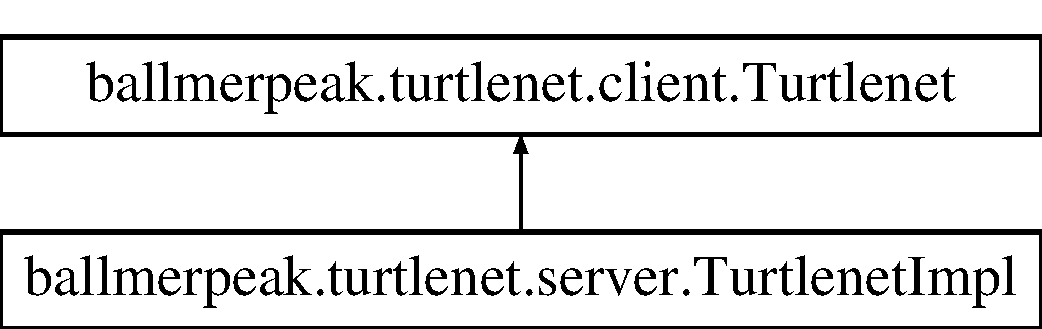
\includegraphics[height=2.000000cm]{interfaceballmerpeak_1_1turtlenet_1_1client_1_1Turtlenet}
\end{center}
\end{figure}
\subsubsection*{Public Member Functions}
\begin{DoxyCompactItemize}
\item 
\hypertarget{interfaceballmerpeak_1_1turtlenet_1_1client_1_1Turtlenet_ad2c185cc33495082c8da75b56de3923d}{String {\bfseries start\-T\-N} (String password)}\label{interfaceballmerpeak_1_1turtlenet_1_1client_1_1Turtlenet_ad2c185cc33495082c8da75b56de3923d}

\item 
\hypertarget{interfaceballmerpeak_1_1turtlenet_1_1client_1_1Turtlenet_ab9c5f257cca5e02901ffd588965963be}{String {\bfseries stop\-T\-N} ()}\label{interfaceballmerpeak_1_1turtlenet_1_1client_1_1Turtlenet_ab9c5f257cca5e02901ffd588965963be}

\item 
\hypertarget{interfaceballmerpeak_1_1turtlenet_1_1client_1_1Turtlenet_af9208c1d9cb46ce3470a33df4a1a4df9}{String {\bfseries is\-First\-Time} ()}\label{interfaceballmerpeak_1_1turtlenet_1_1client_1_1Turtlenet_af9208c1d9cb46ce3470a33df4a1a4df9}

\item 
\hypertarget{interfaceballmerpeak_1_1turtlenet_1_1client_1_1Turtlenet_ad64cfc9925dcd72033616bbdb04949a0}{String {\bfseries register} (String username, String password)}\label{interfaceballmerpeak_1_1turtlenet_1_1client_1_1Turtlenet_ad64cfc9925dcd72033616bbdb04949a0}

\item 
\hypertarget{interfaceballmerpeak_1_1turtlenet_1_1client_1_1Turtlenet_a7be22b6c4de115ee3842215390327a01}{String {\bfseries get\-Username} (String key)}\label{interfaceballmerpeak_1_1turtlenet_1_1client_1_1Turtlenet_a7be22b6c4de115ee3842215390327a01}

\item 
\hypertarget{interfaceballmerpeak_1_1turtlenet_1_1client_1_1Turtlenet_a1403ccfe05dbc6d8c1634b9ee495db15}{String {\bfseries get\-My\-Username} ()}\label{interfaceballmerpeak_1_1turtlenet_1_1client_1_1Turtlenet_a1403ccfe05dbc6d8c1634b9ee495db15}

\item 
\hypertarget{interfaceballmerpeak_1_1turtlenet_1_1client_1_1Turtlenet_ad8ee0ed3492a6014119f93e924f7e08c}{String {\bfseries get\-P\-D\-A\-T\-A} (String field, String key)}\label{interfaceballmerpeak_1_1turtlenet_1_1client_1_1Turtlenet_ad8ee0ed3492a6014119f93e924f7e08c}

\item 
\hypertarget{interfaceballmerpeak_1_1turtlenet_1_1client_1_1Turtlenet_a6e1aec0d0b894cc034a058e6a1e59f8d}{String {\bfseries get\-My\-P\-D\-A\-T\-A} (String field)}\label{interfaceballmerpeak_1_1turtlenet_1_1client_1_1Turtlenet_a6e1aec0d0b894cc034a058e6a1e59f8d}

\item 
\hypertarget{interfaceballmerpeak_1_1turtlenet_1_1client_1_1Turtlenet_a1e027a6781273a6004088c007652bbfb}{String {\bfseries get\-Key} (String username)}\label{interfaceballmerpeak_1_1turtlenet_1_1client_1_1Turtlenet_a1e027a6781273a6004088c007652bbfb}

\item 
\hypertarget{interfaceballmerpeak_1_1turtlenet_1_1client_1_1Turtlenet_a92f271e68b3fe28daaff65852546f0b7}{String {\bfseries get\-My\-Key} ()}\label{interfaceballmerpeak_1_1turtlenet_1_1client_1_1Turtlenet_a92f271e68b3fe28daaff65852546f0b7}

\item 
\hypertarget{interfaceballmerpeak_1_1turtlenet_1_1client_1_1Turtlenet_ac9f6b1c3381cbfe692ec418c5a20de72}{String\mbox{[}$\,$\mbox{]}\mbox{[}$\,$\mbox{]} {\bfseries get\-People} ()}\label{interfaceballmerpeak_1_1turtlenet_1_1client_1_1Turtlenet_ac9f6b1c3381cbfe692ec418c5a20de72}

\item 
\hypertarget{interfaceballmerpeak_1_1turtlenet_1_1client_1_1Turtlenet_a1576427e28630ba76693f57bb6c6e8e5}{String\mbox{[}$\,$\mbox{]}\mbox{[}$\,$\mbox{]} {\bfseries get\-Categories} ()}\label{interfaceballmerpeak_1_1turtlenet_1_1client_1_1Turtlenet_a1576427e28630ba76693f57bb6c6e8e5}

\item 
\hypertarget{interfaceballmerpeak_1_1turtlenet_1_1client_1_1Turtlenet_a672211366da676547b6f23e7cab5b3d2}{String\mbox{[}$\,$\mbox{]}\mbox{[}$\,$\mbox{]} {\bfseries get\-Category\-Members} (String category)}\label{interfaceballmerpeak_1_1turtlenet_1_1client_1_1Turtlenet_a672211366da676547b6f23e7cab5b3d2}

\item 
\hypertarget{interfaceballmerpeak_1_1turtlenet_1_1client_1_1Turtlenet_aee477261c671b6a20237d0fa8ddab7f0}{\hyperlink{classballmerpeak_1_1turtlenet_1_1shared_1_1Conversation}{Conversation} {\bfseries get\-Conversation} (String sig)}\label{interfaceballmerpeak_1_1turtlenet_1_1client_1_1Turtlenet_aee477261c671b6a20237d0fa8ddab7f0}

\item 
\hypertarget{interfaceballmerpeak_1_1turtlenet_1_1client_1_1Turtlenet_a2282dffbbc36f3398c0498c95629056f}{\hyperlink{classballmerpeak_1_1turtlenet_1_1shared_1_1Conversation}{Conversation}\mbox{[}$\,$\mbox{]} {\bfseries get\-Conversations} ()}\label{interfaceballmerpeak_1_1turtlenet_1_1client_1_1Turtlenet_a2282dffbbc36f3398c0498c95629056f}

\item 
\hypertarget{interfaceballmerpeak_1_1turtlenet_1_1client_1_1Turtlenet_a6f2114b1e820a9c8fcfce3c9be6de12b}{String\mbox{[}$\,$\mbox{]}\mbox{[}$\,$\mbox{]} {\bfseries get\-Conversation\-Messages} (String sig)}\label{interfaceballmerpeak_1_1turtlenet_1_1client_1_1Turtlenet_a6f2114b1e820a9c8fcfce3c9be6de12b}

\item 
\hypertarget{interfaceballmerpeak_1_1turtlenet_1_1client_1_1Turtlenet_a162a9e8f6101fc27d58a372735cd3702}{\hyperlink{classballmerpeak_1_1turtlenet_1_1shared_1_1PostDetails}{Post\-Details}\mbox{[}$\,$\mbox{]} {\bfseries get\-Wall\-Posts} (String key)}\label{interfaceballmerpeak_1_1turtlenet_1_1client_1_1Turtlenet_a162a9e8f6101fc27d58a372735cd3702}

\item 
\hypertarget{interfaceballmerpeak_1_1turtlenet_1_1client_1_1Turtlenet_aeae3b123fbfea489eb6888dbc896aaca}{\hyperlink{classballmerpeak_1_1turtlenet_1_1shared_1_1CommentDetails}{Comment\-Details}\mbox{[}$\,$\mbox{]} {\bfseries get\-Comments} (String parent)}\label{interfaceballmerpeak_1_1turtlenet_1_1client_1_1Turtlenet_aeae3b123fbfea489eb6888dbc896aaca}

\item 
\hypertarget{interfaceballmerpeak_1_1turtlenet_1_1client_1_1Turtlenet_a3859f33caf36133dbdb56c306e496f33}{Long {\bfseries time\-Most\-Recent\-Wall\-Post} (String key)}\label{interfaceballmerpeak_1_1turtlenet_1_1client_1_1Turtlenet_a3859f33caf36133dbdb56c306e496f33}

\item 
\hypertarget{interfaceballmerpeak_1_1turtlenet_1_1client_1_1Turtlenet_aef7a6b32445ad461aee9206782e7a23a}{Long {\bfseries get\-Convo\-Last\-Updated} (String sig)}\label{interfaceballmerpeak_1_1turtlenet_1_1client_1_1Turtlenet_aef7a6b32445ad461aee9206782e7a23a}

\item 
\hypertarget{interfaceballmerpeak_1_1turtlenet_1_1client_1_1Turtlenet_afe7fb0ea0aa816d74bf768586a790920}{Long {\bfseries get\-Post\-Last\-Commented} (String sig)}\label{interfaceballmerpeak_1_1turtlenet_1_1client_1_1Turtlenet_afe7fb0ea0aa816d74bf768586a790920}

\item 
\hypertarget{interfaceballmerpeak_1_1turtlenet_1_1client_1_1Turtlenet_ae48f0a9d17c153ea02178f15921adbb3}{String {\bfseries claim\-Username} (String uname)}\label{interfaceballmerpeak_1_1turtlenet_1_1client_1_1Turtlenet_ae48f0a9d17c153ea02178f15921adbb3}

\item 
\hypertarget{interfaceballmerpeak_1_1turtlenet_1_1client_1_1Turtlenet_a7bd4e01c7a9b31062600215c190b2203}{String {\bfseries update\-P\-D\-A\-T\-A} (String field, String new\-Value)}\label{interfaceballmerpeak_1_1turtlenet_1_1client_1_1Turtlenet_a7bd4e01c7a9b31062600215c190b2203}

\item 
\hypertarget{interfaceballmerpeak_1_1turtlenet_1_1client_1_1Turtlenet_a169f35c3f487d0282c9cca1c69ef0864}{String {\bfseries update\-P\-D\-A\-T\-Apermission} (String category, boolean value)}\label{interfaceballmerpeak_1_1turtlenet_1_1client_1_1Turtlenet_a169f35c3f487d0282c9cca1c69ef0864}

\item 
\hypertarget{interfaceballmerpeak_1_1turtlenet_1_1client_1_1Turtlenet_a73d0ea7f23c65c50b767ad11a15eb551}{String\mbox{[}$\,$\mbox{]} {\bfseries create\-C\-H\-A\-T} (String\mbox{[}$\,$\mbox{]} keys)}\label{interfaceballmerpeak_1_1turtlenet_1_1client_1_1Turtlenet_a73d0ea7f23c65c50b767ad11a15eb551}

\item 
\hypertarget{interfaceballmerpeak_1_1turtlenet_1_1client_1_1Turtlenet_a21764196c7d0327729b959b3b989390f}{String {\bfseries add\-Message\-To\-C\-H\-A\-T} (String text, String sig)}\label{interfaceballmerpeak_1_1turtlenet_1_1client_1_1Turtlenet_a21764196c7d0327729b959b3b989390f}

\item 
\hypertarget{interfaceballmerpeak_1_1turtlenet_1_1client_1_1Turtlenet_a53b64b52b96b7867401e49a98ad3c56c}{String {\bfseries like} (String sig)}\label{interfaceballmerpeak_1_1turtlenet_1_1client_1_1Turtlenet_a53b64b52b96b7867401e49a98ad3c56c}

\item 
\hypertarget{interfaceballmerpeak_1_1turtlenet_1_1client_1_1Turtlenet_a06c7c35b8729183e426c463fbff37b6a}{String {\bfseries unlike} (String sig)}\label{interfaceballmerpeak_1_1turtlenet_1_1client_1_1Turtlenet_a06c7c35b8729183e426c463fbff37b6a}

\item 
\hypertarget{interfaceballmerpeak_1_1turtlenet_1_1client_1_1Turtlenet_a2ef6a7f00e36033f8dc013f9a4de2dff}{String {\bfseries add\-Category} (String name)}\label{interfaceballmerpeak_1_1turtlenet_1_1client_1_1Turtlenet_a2ef6a7f00e36033f8dc013f9a4de2dff}

\item 
\hypertarget{interfaceballmerpeak_1_1turtlenet_1_1client_1_1Turtlenet_ae9cd677b3fa8a8a9114297e58047abe3}{String {\bfseries add\-To\-Category} (String category, String key)}\label{interfaceballmerpeak_1_1turtlenet_1_1client_1_1Turtlenet_ae9cd677b3fa8a8a9114297e58047abe3}

\item 
\hypertarget{interfaceballmerpeak_1_1turtlenet_1_1client_1_1Turtlenet_aefdafb728b08fcd230ed1ca26bf4ce9f}{String {\bfseries add\-Key} (String key)}\label{interfaceballmerpeak_1_1turtlenet_1_1client_1_1Turtlenet_aefdafb728b08fcd230ed1ca26bf4ce9f}

\item 
\hypertarget{interfaceballmerpeak_1_1turtlenet_1_1client_1_1Turtlenet_a820a403aab7aeaa167cfef0f9a57c47e}{String {\bfseries add\-Post} (String wall\-Key, String category\-Visible\-To, String msg)}\label{interfaceballmerpeak_1_1turtlenet_1_1client_1_1Turtlenet_a820a403aab7aeaa167cfef0f9a57c47e}

\item 
\hypertarget{interfaceballmerpeak_1_1turtlenet_1_1client_1_1Turtlenet_a5b9f57137f7abaca7713840d42918434}{String {\bfseries add\-Comment} (String parent, String text)}\label{interfaceballmerpeak_1_1turtlenet_1_1client_1_1Turtlenet_a5b9f57137f7abaca7713840d42918434}

\item 
\hypertarget{interfaceballmerpeak_1_1turtlenet_1_1client_1_1Turtlenet_a3428354990f73f31969b9965ac84f279}{String {\bfseries remove\-From\-Category} (String group, String key)}\label{interfaceballmerpeak_1_1turtlenet_1_1client_1_1Turtlenet_a3428354990f73f31969b9965ac84f279}

\item 
\hypertarget{interfaceballmerpeak_1_1turtlenet_1_1client_1_1Turtlenet_a8630df1f1be5f09e7a258d2f8ab00feb}{String {\bfseries revoke\-My\-Key} ()}\label{interfaceballmerpeak_1_1turtlenet_1_1client_1_1Turtlenet_a8630df1f1be5f09e7a258d2f8ab00feb}

\end{DoxyCompactItemize}


\subsubsection{Detailed Description}


Definition at line 11 of file Turtlenet.\-java.



The documentation for this interface was generated from the following file\-:\begin{DoxyCompactItemize}
\item 
src/ballmerpeak/turtlenet/client/Turtlenet.\-java\end{DoxyCompactItemize}

\hypertarget{interfaceballmerpeak_1_1turtlenet_1_1client_1_1TurtlenetAsync}{\subsection{ballmerpeak.\-turtlenet.\-client.\-Turtlenet\-Async Interface Reference}
\label{interfaceballmerpeak_1_1turtlenet_1_1client_1_1TurtlenetAsync}\index{ballmerpeak.\-turtlenet.\-client.\-Turtlenet\-Async@{ballmerpeak.\-turtlenet.\-client.\-Turtlenet\-Async}}
}
\subsubsection*{Public Member Functions}
\begin{DoxyCompactItemize}
\item 
\hypertarget{interfaceballmerpeak_1_1turtlenet_1_1client_1_1TurtlenetAsync_a7e875c3b32ebacefaffa6ebd69aa2f44}{void {\bfseries start\-T\-N} (String password, Async\-Callback$<$ String $>$ callback)}\label{interfaceballmerpeak_1_1turtlenet_1_1client_1_1TurtlenetAsync_a7e875c3b32ebacefaffa6ebd69aa2f44}

\item 
\hypertarget{interfaceballmerpeak_1_1turtlenet_1_1client_1_1TurtlenetAsync_a70baaa36490a38c7e74cd9f57358336e}{void {\bfseries stop\-T\-N} (Async\-Callback$<$ String $>$ callback)}\label{interfaceballmerpeak_1_1turtlenet_1_1client_1_1TurtlenetAsync_a70baaa36490a38c7e74cd9f57358336e}

\item 
\hypertarget{interfaceballmerpeak_1_1turtlenet_1_1client_1_1TurtlenetAsync_ab4af3d58c26899d68d862bd720624a89}{void {\bfseries is\-First\-Time} (Async\-Callback$<$ String $>$ callback)}\label{interfaceballmerpeak_1_1turtlenet_1_1client_1_1TurtlenetAsync_ab4af3d58c26899d68d862bd720624a89}

\item 
\hypertarget{interfaceballmerpeak_1_1turtlenet_1_1client_1_1TurtlenetAsync_a9190e36e28740c7d668894192b7f2426}{void {\bfseries register} (String username, String password, Async\-Callback$<$ String $>$ callback)}\label{interfaceballmerpeak_1_1turtlenet_1_1client_1_1TurtlenetAsync_a9190e36e28740c7d668894192b7f2426}

\item 
\hypertarget{interfaceballmerpeak_1_1turtlenet_1_1client_1_1TurtlenetAsync_a95d3fddff52812d79a984b9ef91c80ef}{void {\bfseries get\-Username} (String key, Async\-Callback$<$ String $>$ callback)}\label{interfaceballmerpeak_1_1turtlenet_1_1client_1_1TurtlenetAsync_a95d3fddff52812d79a984b9ef91c80ef}

\item 
\hypertarget{interfaceballmerpeak_1_1turtlenet_1_1client_1_1TurtlenetAsync_a07b7f0d56105f4fc945a854a9a316e1e}{void {\bfseries get\-My\-Username} (Async\-Callback$<$ String $>$ callback)}\label{interfaceballmerpeak_1_1turtlenet_1_1client_1_1TurtlenetAsync_a07b7f0d56105f4fc945a854a9a316e1e}

\item 
\hypertarget{interfaceballmerpeak_1_1turtlenet_1_1client_1_1TurtlenetAsync_a2c1ffad266ffba1ced9024011b85ef80}{void {\bfseries get\-P\-D\-A\-T\-A} (String field, String pk, Async\-Callback$<$ String $>$ callback)}\label{interfaceballmerpeak_1_1turtlenet_1_1client_1_1TurtlenetAsync_a2c1ffad266ffba1ced9024011b85ef80}

\item 
\hypertarget{interfaceballmerpeak_1_1turtlenet_1_1client_1_1TurtlenetAsync_acdbee21a3c9f37b2454fa81c6f81afe7}{void {\bfseries get\-My\-P\-D\-A\-T\-A} (String pk, Async\-Callback$<$ String $>$ callback)}\label{interfaceballmerpeak_1_1turtlenet_1_1client_1_1TurtlenetAsync_acdbee21a3c9f37b2454fa81c6f81afe7}

\item 
\hypertarget{interfaceballmerpeak_1_1turtlenet_1_1client_1_1TurtlenetAsync_a24536111eeed3b221288938fe085fc4d}{void {\bfseries get\-Key} (String username, Async\-Callback$<$ String $>$ callback)}\label{interfaceballmerpeak_1_1turtlenet_1_1client_1_1TurtlenetAsync_a24536111eeed3b221288938fe085fc4d}

\item 
\hypertarget{interfaceballmerpeak_1_1turtlenet_1_1client_1_1TurtlenetAsync_a5b01546855375c628581de60cb818bc1}{void {\bfseries get\-My\-Key} (Async\-Callback$<$ String $>$ callback)}\label{interfaceballmerpeak_1_1turtlenet_1_1client_1_1TurtlenetAsync_a5b01546855375c628581de60cb818bc1}

\item 
\hypertarget{interfaceballmerpeak_1_1turtlenet_1_1client_1_1TurtlenetAsync_adb97f522403e5578f780b08e96e8f36b}{void {\bfseries get\-People} (Async\-Callback$<$ String\mbox{[}$\,$\mbox{]}\mbox{[}$\,$\mbox{]}$>$ callback)}\label{interfaceballmerpeak_1_1turtlenet_1_1client_1_1TurtlenetAsync_adb97f522403e5578f780b08e96e8f36b}

\item 
\hypertarget{interfaceballmerpeak_1_1turtlenet_1_1client_1_1TurtlenetAsync_aaefb47d63b1bda3ce692fda9d4ff3b95}{void {\bfseries get\-Categories} (Async\-Callback$<$ String\mbox{[}$\,$\mbox{]}\mbox{[}$\,$\mbox{]}$>$ callback)}\label{interfaceballmerpeak_1_1turtlenet_1_1client_1_1TurtlenetAsync_aaefb47d63b1bda3ce692fda9d4ff3b95}

\item 
\hypertarget{interfaceballmerpeak_1_1turtlenet_1_1client_1_1TurtlenetAsync_a79c59f68c6b1293bb55ba7f7f07bf83a}{void {\bfseries get\-Category\-Members} (String category, Async\-Callback$<$ String\mbox{[}$\,$\mbox{]}\mbox{[}$\,$\mbox{]}$>$ callback)}\label{interfaceballmerpeak_1_1turtlenet_1_1client_1_1TurtlenetAsync_a79c59f68c6b1293bb55ba7f7f07bf83a}

\item 
\hypertarget{interfaceballmerpeak_1_1turtlenet_1_1client_1_1TurtlenetAsync_a2e727bd389829fcebaad120ee7900180}{void {\bfseries get\-Conversation} (String sig, Async\-Callback$<$ \hyperlink{classballmerpeak_1_1turtlenet_1_1shared_1_1Conversation}{Conversation} $>$ callback)}\label{interfaceballmerpeak_1_1turtlenet_1_1client_1_1TurtlenetAsync_a2e727bd389829fcebaad120ee7900180}

\item 
\hypertarget{interfaceballmerpeak_1_1turtlenet_1_1client_1_1TurtlenetAsync_a90857a2008d7e5029c53234d13a3eb29}{void {\bfseries get\-Conversations} (Async\-Callback$<$ \hyperlink{classballmerpeak_1_1turtlenet_1_1shared_1_1Conversation}{Conversation}\mbox{[}$\,$\mbox{]}$>$ callback)}\label{interfaceballmerpeak_1_1turtlenet_1_1client_1_1TurtlenetAsync_a90857a2008d7e5029c53234d13a3eb29}

\item 
\hypertarget{interfaceballmerpeak_1_1turtlenet_1_1client_1_1TurtlenetAsync_af3d8302be17123744f088078aca3c8f1}{void {\bfseries get\-Conversation\-Messages} (String sig, Async\-Callback$<$ String\mbox{[}$\,$\mbox{]}\mbox{[}$\,$\mbox{]}$>$ callback)}\label{interfaceballmerpeak_1_1turtlenet_1_1client_1_1TurtlenetAsync_af3d8302be17123744f088078aca3c8f1}

\item 
\hypertarget{interfaceballmerpeak_1_1turtlenet_1_1client_1_1TurtlenetAsync_a6abffb3c7b3f85f6601f3df9c6bb5af9}{void {\bfseries get\-Wall\-Posts} (String key, Async\-Callback$<$ \hyperlink{classballmerpeak_1_1turtlenet_1_1shared_1_1PostDetails}{Post\-Details}\mbox{[}$\,$\mbox{]}$>$ callback)}\label{interfaceballmerpeak_1_1turtlenet_1_1client_1_1TurtlenetAsync_a6abffb3c7b3f85f6601f3df9c6bb5af9}

\item 
\hypertarget{interfaceballmerpeak_1_1turtlenet_1_1client_1_1TurtlenetAsync_a962d578b71c4bd469bd7e180c8c03ff9}{void {\bfseries get\-Comments} (String parent, Async\-Callback$<$ \hyperlink{classballmerpeak_1_1turtlenet_1_1shared_1_1CommentDetails}{Comment\-Details}\mbox{[}$\,$\mbox{]}$>$ callback)}\label{interfaceballmerpeak_1_1turtlenet_1_1client_1_1TurtlenetAsync_a962d578b71c4bd469bd7e180c8c03ff9}

\item 
\hypertarget{interfaceballmerpeak_1_1turtlenet_1_1client_1_1TurtlenetAsync_a7c5cf7164c931cc259f2f3d536e4a5b6}{void {\bfseries time\-Most\-Recent\-Wall\-Post} (String key, Async\-Callback$<$ Long $>$ callback)}\label{interfaceballmerpeak_1_1turtlenet_1_1client_1_1TurtlenetAsync_a7c5cf7164c931cc259f2f3d536e4a5b6}

\item 
\hypertarget{interfaceballmerpeak_1_1turtlenet_1_1client_1_1TurtlenetAsync_aeea4d58517cb71624be15cec8b0510de}{void {\bfseries get\-Convo\-Last\-Updated} (String sig, Async\-Callback$<$ Long $>$ callback)}\label{interfaceballmerpeak_1_1turtlenet_1_1client_1_1TurtlenetAsync_aeea4d58517cb71624be15cec8b0510de}

\item 
\hypertarget{interfaceballmerpeak_1_1turtlenet_1_1client_1_1TurtlenetAsync_a834d3273d3a41654fdb00ba979ff150b}{void {\bfseries get\-Post\-Last\-Commented} (String sig, Async\-Callback$<$ Long $>$ callback)}\label{interfaceballmerpeak_1_1turtlenet_1_1client_1_1TurtlenetAsync_a834d3273d3a41654fdb00ba979ff150b}

\item 
\hypertarget{interfaceballmerpeak_1_1turtlenet_1_1client_1_1TurtlenetAsync_a1069bf6f78fede8e4f78a2f2e39df27d}{void {\bfseries claim\-Username} (String uname, Async\-Callback$<$ String $>$ callback)}\label{interfaceballmerpeak_1_1turtlenet_1_1client_1_1TurtlenetAsync_a1069bf6f78fede8e4f78a2f2e39df27d}

\item 
\hypertarget{interfaceballmerpeak_1_1turtlenet_1_1client_1_1TurtlenetAsync_a7a7cbb0b042da41c7eeadd290b42a35d}{void {\bfseries update\-P\-D\-A\-T\-A} (String field, String value, Async\-Callback$<$ String $>$ callback)}\label{interfaceballmerpeak_1_1turtlenet_1_1client_1_1TurtlenetAsync_a7a7cbb0b042da41c7eeadd290b42a35d}

\item 
\hypertarget{interfaceballmerpeak_1_1turtlenet_1_1client_1_1TurtlenetAsync_a148056124adb3370e75cafef6f938775}{void {\bfseries update\-P\-D\-A\-T\-Apermission} (String category, boolean value, Async\-Callback$<$ String $>$ callback)}\label{interfaceballmerpeak_1_1turtlenet_1_1client_1_1TurtlenetAsync_a148056124adb3370e75cafef6f938775}

\item 
\hypertarget{interfaceballmerpeak_1_1turtlenet_1_1client_1_1TurtlenetAsync_a107ee449c88dfac657425fdb5933ba93}{void {\bfseries create\-C\-H\-A\-T} (String\mbox{[}$\,$\mbox{]} keys, Async\-Callback$<$ String\mbox{[}$\,$\mbox{]}$>$ callback)}\label{interfaceballmerpeak_1_1turtlenet_1_1client_1_1TurtlenetAsync_a107ee449c88dfac657425fdb5933ba93}

\item 
\hypertarget{interfaceballmerpeak_1_1turtlenet_1_1client_1_1TurtlenetAsync_ad476065edadd8a0adf43a634d89c3ae0}{void {\bfseries add\-Message\-To\-C\-H\-A\-T} (String text, String sig, Async\-Callback$<$ String $>$ callback)}\label{interfaceballmerpeak_1_1turtlenet_1_1client_1_1TurtlenetAsync_ad476065edadd8a0adf43a634d89c3ae0}

\item 
\hypertarget{interfaceballmerpeak_1_1turtlenet_1_1client_1_1TurtlenetAsync_a43ea6e283792f49da2130d82e2e97d21}{void {\bfseries like} (String sig, Async\-Callback$<$ String $>$ callback)}\label{interfaceballmerpeak_1_1turtlenet_1_1client_1_1TurtlenetAsync_a43ea6e283792f49da2130d82e2e97d21}

\item 
\hypertarget{interfaceballmerpeak_1_1turtlenet_1_1client_1_1TurtlenetAsync_adf69c36b9b3c38a741edf28b3b64792f}{void {\bfseries unlike} (String sig, Async\-Callback$<$ String $>$ callback)}\label{interfaceballmerpeak_1_1turtlenet_1_1client_1_1TurtlenetAsync_adf69c36b9b3c38a741edf28b3b64792f}

\item 
\hypertarget{interfaceballmerpeak_1_1turtlenet_1_1client_1_1TurtlenetAsync_a10e4779298723a1ba9e00664b0d8246a}{void {\bfseries add\-Category} (String name, Async\-Callback$<$ String $>$ callback)}\label{interfaceballmerpeak_1_1turtlenet_1_1client_1_1TurtlenetAsync_a10e4779298723a1ba9e00664b0d8246a}

\item 
\hypertarget{interfaceballmerpeak_1_1turtlenet_1_1client_1_1TurtlenetAsync_a8540db4f0ac20ac80e8bca4346761257}{void {\bfseries add\-To\-Category} (String name, String key, Async\-Callback$<$ String $>$ callback)}\label{interfaceballmerpeak_1_1turtlenet_1_1client_1_1TurtlenetAsync_a8540db4f0ac20ac80e8bca4346761257}

\item 
\hypertarget{interfaceballmerpeak_1_1turtlenet_1_1client_1_1TurtlenetAsync_a165c61e5dc2d3aac741bf47c07186b01}{void {\bfseries add\-Key} (String key, Async\-Callback$<$ String $>$ callback)}\label{interfaceballmerpeak_1_1turtlenet_1_1client_1_1TurtlenetAsync_a165c61e5dc2d3aac741bf47c07186b01}

\item 
\hypertarget{interfaceballmerpeak_1_1turtlenet_1_1client_1_1TurtlenetAsync_a6bc9fd822a1776de7cb42561e567cc18}{void {\bfseries add\-Post} (String key, String category\-Visible\-To, String msg, Async\-Callback$<$ String $>$ callback)}\label{interfaceballmerpeak_1_1turtlenet_1_1client_1_1TurtlenetAsync_a6bc9fd822a1776de7cb42561e567cc18}

\item 
\hypertarget{interfaceballmerpeak_1_1turtlenet_1_1client_1_1TurtlenetAsync_a83a5d15e18989bb17ac0bc36d4112dc9}{void {\bfseries add\-Comment} (String parent, String text, Async\-Callback$<$ String $>$ callback)}\label{interfaceballmerpeak_1_1turtlenet_1_1client_1_1TurtlenetAsync_a83a5d15e18989bb17ac0bc36d4112dc9}

\item 
\hypertarget{interfaceballmerpeak_1_1turtlenet_1_1client_1_1TurtlenetAsync_a9b2834a568cdf734a62200928a259eb2}{void {\bfseries remove\-From\-Category} (String group, String key, Async\-Callback$<$ String $>$ callback)}\label{interfaceballmerpeak_1_1turtlenet_1_1client_1_1TurtlenetAsync_a9b2834a568cdf734a62200928a259eb2}

\item 
\hypertarget{interfaceballmerpeak_1_1turtlenet_1_1client_1_1TurtlenetAsync_a03d97f6d5e9f45f538af9c45eb460b94}{void {\bfseries revoke\-My\-Key} (Async\-Callback$<$ String $>$ callback)}\label{interfaceballmerpeak_1_1turtlenet_1_1client_1_1TurtlenetAsync_a03d97f6d5e9f45f538af9c45eb460b94}

\end{DoxyCompactItemize}


\subsubsection{Detailed Description}


Definition at line 9 of file Turtlenet\-Async.\-java.



The documentation for this interface was generated from the following file\-:\begin{DoxyCompactItemize}
\item 
src/ballmerpeak/turtlenet/client/Turtlenet\-Async.\-java\end{DoxyCompactItemize}

\hypertarget{classballmerpeak_1_1turtlenet_1_1server_1_1TurtlenetImpl}{\subsection{ballmerpeak.\-turtlenet.\-server.\-Turtlenet\-Impl Class Reference}
\label{classballmerpeak_1_1turtlenet_1_1server_1_1TurtlenetImpl}\index{ballmerpeak.\-turtlenet.\-server.\-Turtlenet\-Impl@{ballmerpeak.\-turtlenet.\-server.\-Turtlenet\-Impl}}
}


Inherits Remote\-Service\-Servlet, and Turtlenet.

\subsubsection*{Public Member Functions}
\begin{DoxyCompactItemize}
\item 
String \hyperlink{classballmerpeak_1_1turtlenet_1_1server_1_1TurtlenetImpl_ae95fc767bafaeab9ba8fd2ce0ace0dde}{start\-T\-N} (String password)
\begin{DoxyCompactList}\small\item\em Starts Turtlenet client on the backend. \end{DoxyCompactList}\item 
String \hyperlink{classballmerpeak_1_1turtlenet_1_1server_1_1TurtlenetImpl_a5a81c607293705d6bc5a9b5c087ef411}{stop\-T\-N} ()
\begin{DoxyCompactList}\small\item\em Stops Turtlenet client on the backend. \end{DoxyCompactList}\item 
String \hyperlink{classballmerpeak_1_1turtlenet_1_1server_1_1TurtlenetImpl_a64ed53b1b7c02e2a7869dba9a9adeb6b}{is\-First\-Time} ()
\begin{DoxyCompactList}\small\item\em Check if this is the first time Turtlenet has been run. \end{DoxyCompactList}\item 
String \hyperlink{classballmerpeak_1_1turtlenet_1_1server_1_1TurtlenetImpl_ad77aeae77cad163b1fcd099404747f91}{register} (String username, String password)
\begin{DoxyCompactList}\small\item\em Register on the network. \end{DoxyCompactList}\item 
String \hyperlink{classballmerpeak_1_1turtlenet_1_1server_1_1TurtlenetImpl_a4ad92d61008b207cf46dcfdc31e5ea22}{get\-My\-Username} ()
\begin{DoxyCompactList}\small\item\em Retreives the users username from the database. \end{DoxyCompactList}\item 
String \hyperlink{classballmerpeak_1_1turtlenet_1_1server_1_1TurtlenetImpl_a89342b1ea50df43e072c154fdd389d1c}{get\-Username} (String key)
\begin{DoxyCompactList}\small\item\em Retreives the most recent username associated with a given key. \end{DoxyCompactList}\item 
String \hyperlink{classballmerpeak_1_1turtlenet_1_1server_1_1TurtlenetImpl_acc52a5b5a58896bf97348ccd506acb5c}{get\-My\-P\-D\-A\-T\-A} (String field)
\begin{DoxyCompactList}\small\item\em Gets the specified piece of profile data for the current user. \end{DoxyCompactList}\item 
String \hyperlink{classballmerpeak_1_1turtlenet_1_1server_1_1TurtlenetImpl_a2488f315ab0410704181e88c19e74b8c}{get\-P\-D\-A\-T\-A} (String field, String key)
\begin{DoxyCompactList}\small\item\em Gets the specified piece of profile data for the specified user. \end{DoxyCompactList}\item 
String \hyperlink{classballmerpeak_1_1turtlenet_1_1server_1_1TurtlenetImpl_a9c718d4f71c51932d61f308049f1f99d}{get\-My\-Key} ()
\begin{DoxyCompactList}\small\item\em Retrieve the key of the current user. \end{DoxyCompactList}\item 
String \hyperlink{classballmerpeak_1_1turtlenet_1_1server_1_1TurtlenetImpl_a780b106db510694aaa9156d47c09ab05}{get\-Key} (String username)
\begin{DoxyCompactList}\small\item\em Retrieve the key of the specified user. \end{DoxyCompactList}\item 
String\mbox{[}$\,$\mbox{]}\mbox{[}$\,$\mbox{]} \hyperlink{classballmerpeak_1_1turtlenet_1_1server_1_1TurtlenetImpl_aa1c659a0e4d6d60761b3f324cbe7bd8c}{get\-Categories} ()
\begin{DoxyCompactList}\small\item\em Get a list of all categories. \end{DoxyCompactList}\item 
String\mbox{[}$\,$\mbox{]}\mbox{[}$\,$\mbox{]} \hyperlink{classballmerpeak_1_1turtlenet_1_1server_1_1TurtlenetImpl_a5c033785fd6e598229c23c5c08b805ba}{get\-People} ()
\begin{DoxyCompactList}\small\item\em Get all people you know about. \end{DoxyCompactList}\item 
\hyperlink{classballmerpeak_1_1turtlenet_1_1shared_1_1Conversation}{Conversation}\mbox{[}$\,$\mbox{]} \hyperlink{classballmerpeak_1_1turtlenet_1_1server_1_1TurtlenetImpl_a3b7c5b806f0a79198d3042964bf614c1}{get\-Conversations} ()
\begin{DoxyCompactList}\small\item\em Get all conversations you know about. \end{DoxyCompactList}\item 
\hyperlink{classballmerpeak_1_1turtlenet_1_1shared_1_1Conversation}{Conversation} \hyperlink{classballmerpeak_1_1turtlenet_1_1server_1_1TurtlenetImpl_a70dcea522454279983e72b0fd5c3e9a6}{get\-Conversation} (String sig)
\begin{DoxyCompactList}\small\item\em Get details of a specific conversation, but not the messages therein. \end{DoxyCompactList}\item 
String\mbox{[}$\,$\mbox{]}\mbox{[}$\,$\mbox{]} \hyperlink{classballmerpeak_1_1turtlenet_1_1server_1_1TurtlenetImpl_ac92b6c500d8f9f2b0457e99005bf7674}{get\-Conversation\-Messages} (String sig)
\begin{DoxyCompactList}\small\item\em Get all the messages from a given conversation. \end{DoxyCompactList}\item 
String\mbox{[}$\,$\mbox{]}\mbox{[}$\,$\mbox{]} \hyperlink{classballmerpeak_1_1turtlenet_1_1server_1_1TurtlenetImpl_a4ec6b30f0a39631b060273ce493e3a22}{get\-Category\-Members} (String category)
\begin{DoxyCompactList}\small\item\em Get all members of a given category. \end{DoxyCompactList}\item 
\hyperlink{classballmerpeak_1_1turtlenet_1_1shared_1_1PostDetails}{Post\-Details}\mbox{[}$\,$\mbox{]} \hyperlink{classballmerpeak_1_1turtlenet_1_1server_1_1TurtlenetImpl_a25cd6a95e1664bd10cac1ecad0c985df}{get\-Wall\-Posts} (String key)
\begin{DoxyCompactList}\small\item\em Get the posts on the wall of the given user. \end{DoxyCompactList}\item 
\hyperlink{classballmerpeak_1_1turtlenet_1_1shared_1_1CommentDetails}{Comment\-Details}\mbox{[}$\,$\mbox{]} \hyperlink{classballmerpeak_1_1turtlenet_1_1server_1_1TurtlenetImpl_a8ce303e4ed5dd6b459c28595c4fe53a4}{get\-Comments} (String parent)
\begin{DoxyCompactList}\small\item\em Get the details of all comments on a given post or comment. \end{DoxyCompactList}\item 
Long \hyperlink{classballmerpeak_1_1turtlenet_1_1server_1_1TurtlenetImpl_a0555da815949426da19e4aa94798fb77}{time\-Most\-Recent\-Wall\-Post} (String key)
\begin{DoxyCompactList}\small\item\em Get the time that a given users wall was last posted on. \end{DoxyCompactList}\item 
Long \hyperlink{classballmerpeak_1_1turtlenet_1_1server_1_1TurtlenetImpl_a9215bd0cbe7b6c5e925867c7a8ab4be3}{get\-Convo\-Last\-Updated} (String sig)
\begin{DoxyCompactList}\small\item\em Get the time that a given conversation was last posted in. \end{DoxyCompactList}\item 
Long \hyperlink{classballmerpeak_1_1turtlenet_1_1server_1_1TurtlenetImpl_ac98d21dc081755ae7ec66220a0287551}{get\-Post\-Last\-Commented} (String sig)
\begin{DoxyCompactList}\small\item\em Get the time that a given comment or post was last commented on. \end{DoxyCompactList}\item 
String \hyperlink{classballmerpeak_1_1turtlenet_1_1server_1_1TurtlenetImpl_a614a4363b79719b16cc10d9871807326}{claim\-Username} (String uname)
\begin{DoxyCompactList}\small\item\em Register a new username on the network. \end{DoxyCompactList}\item 
String \hyperlink{classballmerpeak_1_1turtlenet_1_1server_1_1TurtlenetImpl_a6498adb8c069a9778b241dde8bad667a}{update\-P\-D\-A\-T\-A} (String field, String value)
\begin{DoxyCompactList}\small\item\em Change your profile information. \end{DoxyCompactList}\item 
String \hyperlink{classballmerpeak_1_1turtlenet_1_1server_1_1TurtlenetImpl_af50db109b6ae5adde4ac18a324a4aa66}{update\-P\-D\-A\-T\-Apermission} (String category, boolean value)
\begin{DoxyCompactList}\small\item\em Change whether or not a category can see your profile information. \end{DoxyCompactList}\item 
String\mbox{[}$\,$\mbox{]} \hyperlink{classballmerpeak_1_1turtlenet_1_1server_1_1TurtlenetImpl_a9dc47df7e7847ac053c189f38b9c7b14}{create\-C\-H\-A\-T} (String\mbox{[}$\,$\mbox{]} keys)
\begin{DoxyCompactList}\small\item\em Create a new conversation. \end{DoxyCompactList}\item 
String \hyperlink{classballmerpeak_1_1turtlenet_1_1server_1_1TurtlenetImpl_a89238dc6ef01ca846a4b616a1d510f85}{add\-Message\-To\-C\-H\-A\-T} (String text, String sig)
\begin{DoxyCompactList}\small\item\em Add a message to a conversation. \end{DoxyCompactList}\item 
String \hyperlink{classballmerpeak_1_1turtlenet_1_1server_1_1TurtlenetImpl_ab806c36948df3c570656cd02025f5188}{like} (String sig)
\begin{DoxyCompactList}\small\item\em Add a like to a post or comment. \end{DoxyCompactList}\item 
String \hyperlink{classballmerpeak_1_1turtlenet_1_1server_1_1TurtlenetImpl_a34dd5b2e3422a38ddd9ab2ded072e870}{unlike} (String sig)
\begin{DoxyCompactList}\small\item\em Remove a like from a post or comment. \end{DoxyCompactList}\item 
String \hyperlink{classballmerpeak_1_1turtlenet_1_1server_1_1TurtlenetImpl_abb2702210515c425be14f39584f761db}{add\-Category} (String name)
\begin{DoxyCompactList}\small\item\em Add a category. \end{DoxyCompactList}\item 
String \hyperlink{classballmerpeak_1_1turtlenet_1_1server_1_1TurtlenetImpl_af382d8d355b9a479d9c047fd9ae722ac}{add\-To\-Category} (String group, String key)
\begin{DoxyCompactList}\small\item\em Add a user to a category. \end{DoxyCompactList}\item 
String \hyperlink{classballmerpeak_1_1turtlenet_1_1server_1_1TurtlenetImpl_a2436ebfe8ae7ed08b831f21f83aaf3bc}{send\-P\-D\-A\-T\-A} (String key)
\begin{DoxyCompactList}\small\item\em Send profile information to the specified key. \end{DoxyCompactList}\item 
String \hyperlink{classballmerpeak_1_1turtlenet_1_1server_1_1TurtlenetImpl_ae8181f4e329a9ffa1d1b4d5deebf617d}{remove\-From\-Category} (String group, String key)
\begin{DoxyCompactList}\small\item\em Remove a user from a category. \end{DoxyCompactList}\item 
String \hyperlink{classballmerpeak_1_1turtlenet_1_1server_1_1TurtlenetImpl_ac32167a339c28603b6166f7dc605f6b8}{add\-Key} (String key)
\begin{DoxyCompactList}\small\item\em Add a public key. \end{DoxyCompactList}\item 
String \hyperlink{classballmerpeak_1_1turtlenet_1_1server_1_1TurtlenetImpl_ae66b52ba9debe2a2f06e6402d485526c}{add\-Post} (String wall\-Key, String category\-Visible\-To, String msg)
\begin{DoxyCompactList}\small\item\em Add a post to a specified wall. \end{DoxyCompactList}\item 
String \hyperlink{classballmerpeak_1_1turtlenet_1_1server_1_1TurtlenetImpl_a0a6b4c30111bf1c85613b2370c20f464}{add\-Comment} (String parent, String text)
\begin{DoxyCompactList}\small\item\em Add a comment to a specified comment or post. \end{DoxyCompactList}\item 
String \hyperlink{classballmerpeak_1_1turtlenet_1_1server_1_1TurtlenetImpl_a2f380c86cd6789269b156b3a731834ae}{revoke\-My\-Key} ()
\begin{DoxyCompactList}\small\item\em Revoke the current users key. \end{DoxyCompactList}\end{DoxyCompactItemize}
\subsubsection*{Package Attributes}
\begin{DoxyCompactItemize}
\item 
\hypertarget{classballmerpeak_1_1turtlenet_1_1server_1_1TurtlenetImpl_a8e8797ccc45aa68a72f8349c4eaf84ca}{\hyperlink{classballmerpeak_1_1turtlenet_1_1server_1_1TNClient}{T\-N\-Client} \hyperlink{classballmerpeak_1_1turtlenet_1_1server_1_1TurtlenetImpl_a8e8797ccc45aa68a72f8349c4eaf84ca}{c} = null}\label{classballmerpeak_1_1turtlenet_1_1server_1_1TurtlenetImpl_a8e8797ccc45aa68a72f8349c4eaf84ca}

\begin{DoxyCompactList}\small\item\em Turtlenet client that runs in the background on the backend. \end{DoxyCompactList}\end{DoxyCompactItemize}


\subsubsection{Detailed Description}


Definition at line 15 of file Turtlenet\-Impl.\-java.



\subsubsection{Member Function Documentation}
\hypertarget{classballmerpeak_1_1turtlenet_1_1server_1_1TurtlenetImpl_abb2702210515c425be14f39584f761db}{\index{ballmerpeak\-::turtlenet\-::server\-::\-Turtlenet\-Impl@{ballmerpeak\-::turtlenet\-::server\-::\-Turtlenet\-Impl}!add\-Category@{add\-Category}}
\index{add\-Category@{add\-Category}!ballmerpeak::turtlenet::server::TurtlenetImpl@{ballmerpeak\-::turtlenet\-::server\-::\-Turtlenet\-Impl}}
\paragraph[{add\-Category}]{\setlength{\rightskip}{0pt plus 5cm}String ballmerpeak.\-turtlenet.\-server.\-Turtlenet\-Impl.\-add\-Category (
\begin{DoxyParamCaption}
\item[{String}]{name}
\end{DoxyParamCaption}
)}}\label{classballmerpeak_1_1turtlenet_1_1server_1_1TurtlenetImpl_abb2702210515c425be14f39584f761db}


Add a category. 

By default the category cannot see your profile information. 
\begin{DoxyParams}{Parameters}
{\em name} & The name of the category you wish to create. \\
\hline
\end{DoxyParams}
\begin{DoxyReturn}{Returns}
\char`\"{}true\char`\"{} if successful, \char`\"{}false\char`\"{} otherwise. 
\end{DoxyReturn}


Definition at line 480 of file Turtlenet\-Impl.\-java.

\hypertarget{classballmerpeak_1_1turtlenet_1_1server_1_1TurtlenetImpl_a0a6b4c30111bf1c85613b2370c20f464}{\index{ballmerpeak\-::turtlenet\-::server\-::\-Turtlenet\-Impl@{ballmerpeak\-::turtlenet\-::server\-::\-Turtlenet\-Impl}!add\-Comment@{add\-Comment}}
\index{add\-Comment@{add\-Comment}!ballmerpeak::turtlenet::server::TurtlenetImpl@{ballmerpeak\-::turtlenet\-::server\-::\-Turtlenet\-Impl}}
\paragraph[{add\-Comment}]{\setlength{\rightskip}{0pt plus 5cm}String ballmerpeak.\-turtlenet.\-server.\-Turtlenet\-Impl.\-add\-Comment (
\begin{DoxyParamCaption}
\item[{String}]{parent, }
\item[{String}]{text}
\end{DoxyParamCaption}
)}}\label{classballmerpeak_1_1turtlenet_1_1server_1_1TurtlenetImpl_a0a6b4c30111bf1c85613b2370c20f464}


Add a comment to a specified comment or post. 

Commenting does not require the permission of the person who posted the item you are commenting. 
\begin{DoxyParams}{Parameters}
{\em parent} & The signature of the post or comment that you wish to comment on. \\
\hline
{\em text} & The text of the comment you wish to make. \\
\hline
\end{DoxyParams}
\begin{DoxyReturn}{Returns}
\char`\"{}true\char`\"{} if successful, \char`\"{}false\char`\"{} otherwise. 
\end{DoxyReturn}


Definition at line 598 of file Turtlenet\-Impl.\-java.

\hypertarget{classballmerpeak_1_1turtlenet_1_1server_1_1TurtlenetImpl_ac32167a339c28603b6166f7dc605f6b8}{\index{ballmerpeak\-::turtlenet\-::server\-::\-Turtlenet\-Impl@{ballmerpeak\-::turtlenet\-::server\-::\-Turtlenet\-Impl}!add\-Key@{add\-Key}}
\index{add\-Key@{add\-Key}!ballmerpeak::turtlenet::server::TurtlenetImpl@{ballmerpeak\-::turtlenet\-::server\-::\-Turtlenet\-Impl}}
\paragraph[{add\-Key}]{\setlength{\rightskip}{0pt plus 5cm}String ballmerpeak.\-turtlenet.\-server.\-Turtlenet\-Impl.\-add\-Key (
\begin{DoxyParamCaption}
\item[{String}]{key}
\end{DoxyParamCaption}
)}}\label{classballmerpeak_1_1turtlenet_1_1server_1_1TurtlenetImpl_ac32167a339c28603b6166f7dc605f6b8}


Add a public key. 


\begin{DoxyParams}{Parameters}
{\em key} & The key you wish to add. \\
\hline
\end{DoxyParams}
\begin{DoxyReturn}{Returns}
\char`\"{}true\char`\"{} if successful, \char`\"{}false\char`\"{} otherwise. 
\end{DoxyReturn}


Definition at line 555 of file Turtlenet\-Impl.\-java.

\hypertarget{classballmerpeak_1_1turtlenet_1_1server_1_1TurtlenetImpl_a89238dc6ef01ca846a4b616a1d510f85}{\index{ballmerpeak\-::turtlenet\-::server\-::\-Turtlenet\-Impl@{ballmerpeak\-::turtlenet\-::server\-::\-Turtlenet\-Impl}!add\-Message\-To\-C\-H\-A\-T@{add\-Message\-To\-C\-H\-A\-T}}
\index{add\-Message\-To\-C\-H\-A\-T@{add\-Message\-To\-C\-H\-A\-T}!ballmerpeak::turtlenet::server::TurtlenetImpl@{ballmerpeak\-::turtlenet\-::server\-::\-Turtlenet\-Impl}}
\paragraph[{add\-Message\-To\-C\-H\-A\-T}]{\setlength{\rightskip}{0pt plus 5cm}String ballmerpeak.\-turtlenet.\-server.\-Turtlenet\-Impl.\-add\-Message\-To\-C\-H\-A\-T (
\begin{DoxyParamCaption}
\item[{String}]{text, }
\item[{String}]{sig}
\end{DoxyParamCaption}
)}}\label{classballmerpeak_1_1turtlenet_1_1server_1_1TurtlenetImpl_a89238dc6ef01ca846a4b616a1d510f85}


Add a message to a conversation. 


\begin{DoxyParams}{Parameters}
{\em text} & The text of your message. \\
\hline
{\em sig} & The signature of the conversation you wish to add a message to. \\
\hline
\end{DoxyParams}
\begin{DoxyReturn}{Returns}
\char`\"{}true\char`\"{} if successful, \char`\"{}false\char`\"{} otherwise. 
\end{DoxyReturn}


Definition at line 416 of file Turtlenet\-Impl.\-java.

\hypertarget{classballmerpeak_1_1turtlenet_1_1server_1_1TurtlenetImpl_ae66b52ba9debe2a2f06e6402d485526c}{\index{ballmerpeak\-::turtlenet\-::server\-::\-Turtlenet\-Impl@{ballmerpeak\-::turtlenet\-::server\-::\-Turtlenet\-Impl}!add\-Post@{add\-Post}}
\index{add\-Post@{add\-Post}!ballmerpeak::turtlenet::server::TurtlenetImpl@{ballmerpeak\-::turtlenet\-::server\-::\-Turtlenet\-Impl}}
\paragraph[{add\-Post}]{\setlength{\rightskip}{0pt plus 5cm}String ballmerpeak.\-turtlenet.\-server.\-Turtlenet\-Impl.\-add\-Post (
\begin{DoxyParamCaption}
\item[{String}]{wall\-Key, }
\item[{String}]{category\-Visible\-To, }
\item[{String}]{msg}
\end{DoxyParamCaption}
)}}\label{classballmerpeak_1_1turtlenet_1_1server_1_1TurtlenetImpl_ae66b52ba9debe2a2f06e6402d485526c}


Add a post to a specified wall. 

Posting on another users wall does not require their permission. 
\begin{DoxyParams}{Parameters}
{\em wall\-Key} & The key of the user whos wall you want to post on. \\
\hline
{\em category\-Visible\-To} & The name of the category of people who may see the post. \\
\hline
{\em msg} & The text of the post you wish to make. \\
\hline
\end{DoxyParams}
\begin{DoxyReturn}{Returns}
\char`\"{}true\char`\"{} if successful, \char`\"{}false\char`\"{} otherwise. 
\end{DoxyReturn}


Definition at line 570 of file Turtlenet\-Impl.\-java.

\hypertarget{classballmerpeak_1_1turtlenet_1_1server_1_1TurtlenetImpl_af382d8d355b9a479d9c047fd9ae722ac}{\index{ballmerpeak\-::turtlenet\-::server\-::\-Turtlenet\-Impl@{ballmerpeak\-::turtlenet\-::server\-::\-Turtlenet\-Impl}!add\-To\-Category@{add\-To\-Category}}
\index{add\-To\-Category@{add\-To\-Category}!ballmerpeak::turtlenet::server::TurtlenetImpl@{ballmerpeak\-::turtlenet\-::server\-::\-Turtlenet\-Impl}}
\paragraph[{add\-To\-Category}]{\setlength{\rightskip}{0pt plus 5cm}String ballmerpeak.\-turtlenet.\-server.\-Turtlenet\-Impl.\-add\-To\-Category (
\begin{DoxyParamCaption}
\item[{String}]{group, }
\item[{String}]{key}
\end{DoxyParamCaption}
)}}\label{classballmerpeak_1_1turtlenet_1_1server_1_1TurtlenetImpl_af382d8d355b9a479d9c047fd9ae722ac}


Add a user to a category. 


\begin{DoxyParams}{Parameters}
{\em group} & The name of the category you wish to add a user to. \\
\hline
{\em key} & The key you wish to add to the category. \\
\hline
\end{DoxyParams}
\begin{DoxyReturn}{Returns}
\char`\"{}true\char`\"{} if successful, \char`\"{}false\char`\"{} otherwise. 
\end{DoxyReturn}


Definition at line 494 of file Turtlenet\-Impl.\-java.

\hypertarget{classballmerpeak_1_1turtlenet_1_1server_1_1TurtlenetImpl_a614a4363b79719b16cc10d9871807326}{\index{ballmerpeak\-::turtlenet\-::server\-::\-Turtlenet\-Impl@{ballmerpeak\-::turtlenet\-::server\-::\-Turtlenet\-Impl}!claim\-Username@{claim\-Username}}
\index{claim\-Username@{claim\-Username}!ballmerpeak::turtlenet::server::TurtlenetImpl@{ballmerpeak\-::turtlenet\-::server\-::\-Turtlenet\-Impl}}
\paragraph[{claim\-Username}]{\setlength{\rightskip}{0pt plus 5cm}String ballmerpeak.\-turtlenet.\-server.\-Turtlenet\-Impl.\-claim\-Username (
\begin{DoxyParamCaption}
\item[{String}]{uname}
\end{DoxyParamCaption}
)}}\label{classballmerpeak_1_1turtlenet_1_1server_1_1TurtlenetImpl_a614a4363b79719b16cc10d9871807326}


Register a new username on the network. 


\begin{DoxyParams}{Parameters}
{\em uname} & The desired username. \\
\hline
\end{DoxyParams}
\begin{DoxyReturn}{Returns}
\char`\"{}true\char`\"{} if successful, \char`\"{}false\char`\"{} otherwise. Usernames must be unique and the server enforces this. 
\end{DoxyReturn}


Definition at line 309 of file Turtlenet\-Impl.\-java.

\hypertarget{classballmerpeak_1_1turtlenet_1_1server_1_1TurtlenetImpl_a9dc47df7e7847ac053c189f38b9c7b14}{\index{ballmerpeak\-::turtlenet\-::server\-::\-Turtlenet\-Impl@{ballmerpeak\-::turtlenet\-::server\-::\-Turtlenet\-Impl}!create\-C\-H\-A\-T@{create\-C\-H\-A\-T}}
\index{create\-C\-H\-A\-T@{create\-C\-H\-A\-T}!ballmerpeak::turtlenet::server::TurtlenetImpl@{ballmerpeak\-::turtlenet\-::server\-::\-Turtlenet\-Impl}}
\paragraph[{create\-C\-H\-A\-T}]{\setlength{\rightskip}{0pt plus 5cm}String \mbox{[}$\,$\mbox{]} ballmerpeak.\-turtlenet.\-server.\-Turtlenet\-Impl.\-create\-C\-H\-A\-T (
\begin{DoxyParamCaption}
\item[{String\mbox{[}$\,$\mbox{]}}]{keys}
\end{DoxyParamCaption}
)}}\label{classballmerpeak_1_1turtlenet_1_1server_1_1TurtlenetImpl_a9dc47df7e7847ac053c189f38b9c7b14}


Create a new conversation. 


\begin{DoxyParams}{Parameters}
{\em keys} & The keys of each person you wish to include in the conversation. \\
\hline
\end{DoxyParams}
\begin{DoxyReturn}{Returns}
\char`\"{}true\char`\"{} if successful, \char`\"{}false\char`\"{} otherwise. 
\end{DoxyReturn}


Definition at line 369 of file Turtlenet\-Impl.\-java.

\hypertarget{classballmerpeak_1_1turtlenet_1_1server_1_1TurtlenetImpl_aa1c659a0e4d6d60761b3f324cbe7bd8c}{\index{ballmerpeak\-::turtlenet\-::server\-::\-Turtlenet\-Impl@{ballmerpeak\-::turtlenet\-::server\-::\-Turtlenet\-Impl}!get\-Categories@{get\-Categories}}
\index{get\-Categories@{get\-Categories}!ballmerpeak::turtlenet::server::TurtlenetImpl@{ballmerpeak\-::turtlenet\-::server\-::\-Turtlenet\-Impl}}
\paragraph[{get\-Categories}]{\setlength{\rightskip}{0pt plus 5cm}String \mbox{[}$\,$\mbox{]}\mbox{[}$\,$\mbox{]} ballmerpeak.\-turtlenet.\-server.\-Turtlenet\-Impl.\-get\-Categories (
\begin{DoxyParamCaption}
{}
\end{DoxyParamCaption}
)}}\label{classballmerpeak_1_1turtlenet_1_1server_1_1TurtlenetImpl_aa1c659a0e4d6d60761b3f324cbe7bd8c}


Get a list of all categories. 

\begin{DoxyReturn}{Returns}
The names of each category and if it can see your profile info. Data is in this format\-: \{\{\char`\"{}friends\char`\"{}, \char`\"{}false\char`\"{}\}, \{\char`\"{}family\char`\"{}, \char`\"{}true\char`\"{}\}, etc.\} 
\end{DoxyReturn}


Definition at line 149 of file Turtlenet\-Impl.\-java.

\hypertarget{classballmerpeak_1_1turtlenet_1_1server_1_1TurtlenetImpl_a4ec6b30f0a39631b060273ce493e3a22}{\index{ballmerpeak\-::turtlenet\-::server\-::\-Turtlenet\-Impl@{ballmerpeak\-::turtlenet\-::server\-::\-Turtlenet\-Impl}!get\-Category\-Members@{get\-Category\-Members}}
\index{get\-Category\-Members@{get\-Category\-Members}!ballmerpeak::turtlenet::server::TurtlenetImpl@{ballmerpeak\-::turtlenet\-::server\-::\-Turtlenet\-Impl}}
\paragraph[{get\-Category\-Members}]{\setlength{\rightskip}{0pt plus 5cm}String \mbox{[}$\,$\mbox{]}\mbox{[}$\,$\mbox{]} ballmerpeak.\-turtlenet.\-server.\-Turtlenet\-Impl.\-get\-Category\-Members (
\begin{DoxyParamCaption}
\item[{String}]{category}
\end{DoxyParamCaption}
)}}\label{classballmerpeak_1_1turtlenet_1_1server_1_1TurtlenetImpl_a4ec6b30f0a39631b060273ce493e3a22}


Get all members of a given category. 

If the category given is \char`\"{}all\char`\"{} then all known people are returned. 
\begin{DoxyParams}{Parameters}
{\em category} & The name of the category of which you want to know the members. \\
\hline
\end{DoxyParams}
\begin{DoxyReturn}{Returns}
The username and key of each member of the specified category. Data is in this format\-: \{\{\char`\"{}bob\char`\"{}, \char`\"{}bobs\-\_\-key\char`\"{}\}, \{\char`\"{}john\char`\"{}, \char`\"{}johns\-\_\-key\char`\"{}\}, etc.\} 
\end{DoxyReturn}


Definition at line 206 of file Turtlenet\-Impl.\-java.

\hypertarget{classballmerpeak_1_1turtlenet_1_1server_1_1TurtlenetImpl_a8ce303e4ed5dd6b459c28595c4fe53a4}{\index{ballmerpeak\-::turtlenet\-::server\-::\-Turtlenet\-Impl@{ballmerpeak\-::turtlenet\-::server\-::\-Turtlenet\-Impl}!get\-Comments@{get\-Comments}}
\index{get\-Comments@{get\-Comments}!ballmerpeak::turtlenet::server::TurtlenetImpl@{ballmerpeak\-::turtlenet\-::server\-::\-Turtlenet\-Impl}}
\paragraph[{get\-Comments}]{\setlength{\rightskip}{0pt plus 5cm}{\bf Comment\-Details} \mbox{[}$\,$\mbox{]} ballmerpeak.\-turtlenet.\-server.\-Turtlenet\-Impl.\-get\-Comments (
\begin{DoxyParamCaption}
\item[{String}]{parent}
\end{DoxyParamCaption}
)}}\label{classballmerpeak_1_1turtlenet_1_1server_1_1TurtlenetImpl_a8ce303e4ed5dd6b459c28595c4fe53a4}


Get the details of all comments on a given post or comment. 


\begin{DoxyParams}{Parameters}
{\em parent} & The signature of the item whose comments one desires. \\
\hline
\end{DoxyParams}
\begin{DoxyReturn}{Returns}
An array of Comment\-Details, ordered chronologically so that element 0 is the oldest comment on the item. 
\end{DoxyReturn}


Definition at line 247 of file Turtlenet\-Impl.\-java.

\hypertarget{classballmerpeak_1_1turtlenet_1_1server_1_1TurtlenetImpl_a70dcea522454279983e72b0fd5c3e9a6}{\index{ballmerpeak\-::turtlenet\-::server\-::\-Turtlenet\-Impl@{ballmerpeak\-::turtlenet\-::server\-::\-Turtlenet\-Impl}!get\-Conversation@{get\-Conversation}}
\index{get\-Conversation@{get\-Conversation}!ballmerpeak::turtlenet::server::TurtlenetImpl@{ballmerpeak\-::turtlenet\-::server\-::\-Turtlenet\-Impl}}
\paragraph[{get\-Conversation}]{\setlength{\rightskip}{0pt plus 5cm}{\bf Conversation} ballmerpeak.\-turtlenet.\-server.\-Turtlenet\-Impl.\-get\-Conversation (
\begin{DoxyParamCaption}
\item[{String}]{sig}
\end{DoxyParamCaption}
)}}\label{classballmerpeak_1_1turtlenet_1_1server_1_1TurtlenetImpl_a70dcea522454279983e72b0fd5c3e9a6}


Get details of a specific conversation, but not the messages therein. 


\begin{DoxyParams}{Parameters}
{\em sig} & The signature of the conversation you want details about. \\
\hline
\end{DoxyParams}
\begin{DoxyReturn}{Returns}
A conversation object with the details of the specified conversation. 
\end{DoxyReturn}


Definition at line 184 of file Turtlenet\-Impl.\-java.

\hypertarget{classballmerpeak_1_1turtlenet_1_1server_1_1TurtlenetImpl_ac92b6c500d8f9f2b0457e99005bf7674}{\index{ballmerpeak\-::turtlenet\-::server\-::\-Turtlenet\-Impl@{ballmerpeak\-::turtlenet\-::server\-::\-Turtlenet\-Impl}!get\-Conversation\-Messages@{get\-Conversation\-Messages}}
\index{get\-Conversation\-Messages@{get\-Conversation\-Messages}!ballmerpeak::turtlenet::server::TurtlenetImpl@{ballmerpeak\-::turtlenet\-::server\-::\-Turtlenet\-Impl}}
\paragraph[{get\-Conversation\-Messages}]{\setlength{\rightskip}{0pt plus 5cm}String \mbox{[}$\,$\mbox{]}\mbox{[}$\,$\mbox{]} ballmerpeak.\-turtlenet.\-server.\-Turtlenet\-Impl.\-get\-Conversation\-Messages (
\begin{DoxyParamCaption}
\item[{String}]{sig}
\end{DoxyParamCaption}
)}}\label{classballmerpeak_1_1turtlenet_1_1server_1_1TurtlenetImpl_ac92b6c500d8f9f2b0457e99005bf7674}


Get all the messages from a given conversation. 


\begin{DoxyParams}{Parameters}
{\em sig} & The signature of the conversation you want the messages of. \\
\hline
\end{DoxyParams}
\begin{DoxyReturn}{Returns}
The messages in the specified conversation, in chronological order (i.\-e.\-: Element 0 is the oldest message in the conversation). Data is in this format\-: \{\{username, time, msg\}, \{username, time, msg\}, etc.\} 
\end{DoxyReturn}


Definition at line 195 of file Turtlenet\-Impl.\-java.

\hypertarget{classballmerpeak_1_1turtlenet_1_1server_1_1TurtlenetImpl_a3b7c5b806f0a79198d3042964bf614c1}{\index{ballmerpeak\-::turtlenet\-::server\-::\-Turtlenet\-Impl@{ballmerpeak\-::turtlenet\-::server\-::\-Turtlenet\-Impl}!get\-Conversations@{get\-Conversations}}
\index{get\-Conversations@{get\-Conversations}!ballmerpeak::turtlenet::server::TurtlenetImpl@{ballmerpeak\-::turtlenet\-::server\-::\-Turtlenet\-Impl}}
\paragraph[{get\-Conversations}]{\setlength{\rightskip}{0pt plus 5cm}{\bf Conversation} \mbox{[}$\,$\mbox{]} ballmerpeak.\-turtlenet.\-server.\-Turtlenet\-Impl.\-get\-Conversations (
\begin{DoxyParamCaption}
{}
\end{DoxyParamCaption}
)}}\label{classballmerpeak_1_1turtlenet_1_1server_1_1TurtlenetImpl_a3b7c5b806f0a79198d3042964bf614c1}


Get all conversations you know about. 

\begin{DoxyReturn}{Returns}
An array of all conversations you know about in no particular order. 
\end{DoxyReturn}


Definition at line 166 of file Turtlenet\-Impl.\-java.

\hypertarget{classballmerpeak_1_1turtlenet_1_1server_1_1TurtlenetImpl_a9215bd0cbe7b6c5e925867c7a8ab4be3}{\index{ballmerpeak\-::turtlenet\-::server\-::\-Turtlenet\-Impl@{ballmerpeak\-::turtlenet\-::server\-::\-Turtlenet\-Impl}!get\-Convo\-Last\-Updated@{get\-Convo\-Last\-Updated}}
\index{get\-Convo\-Last\-Updated@{get\-Convo\-Last\-Updated}!ballmerpeak::turtlenet::server::TurtlenetImpl@{ballmerpeak\-::turtlenet\-::server\-::\-Turtlenet\-Impl}}
\paragraph[{get\-Convo\-Last\-Updated}]{\setlength{\rightskip}{0pt plus 5cm}Long ballmerpeak.\-turtlenet.\-server.\-Turtlenet\-Impl.\-get\-Convo\-Last\-Updated (
\begin{DoxyParamCaption}
\item[{String}]{sig}
\end{DoxyParamCaption}
)}}\label{classballmerpeak_1_1turtlenet_1_1server_1_1TurtlenetImpl_a9215bd0cbe7b6c5e925867c7a8ab4be3}


Get the time that a given conversation was last posted in. 


\begin{DoxyParams}{Parameters}
{\em sig} & The signature of the conversation being examined. \\
\hline
\end{DoxyParams}
\begin{DoxyReturn}{Returns}
The number of milliseconds from midnight january first 1970 to the time of the most recent message in the specified conversation. 
\end{DoxyReturn}


Definition at line 285 of file Turtlenet\-Impl.\-java.

\hypertarget{classballmerpeak_1_1turtlenet_1_1server_1_1TurtlenetImpl_a780b106db510694aaa9156d47c09ab05}{\index{ballmerpeak\-::turtlenet\-::server\-::\-Turtlenet\-Impl@{ballmerpeak\-::turtlenet\-::server\-::\-Turtlenet\-Impl}!get\-Key@{get\-Key}}
\index{get\-Key@{get\-Key}!ballmerpeak::turtlenet::server::TurtlenetImpl@{ballmerpeak\-::turtlenet\-::server\-::\-Turtlenet\-Impl}}
\paragraph[{get\-Key}]{\setlength{\rightskip}{0pt plus 5cm}String ballmerpeak.\-turtlenet.\-server.\-Turtlenet\-Impl.\-get\-Key (
\begin{DoxyParamCaption}
\item[{String}]{username}
\end{DoxyParamCaption}
)}}\label{classballmerpeak_1_1turtlenet_1_1server_1_1TurtlenetImpl_a780b106db510694aaa9156d47c09ab05}


Retrieve the key of the specified user. 


\begin{DoxyParams}{Parameters}
{\em username} & The username of the user which you wish to know the key of. \\
\hline
\end{DoxyParams}
\begin{DoxyReturn}{Returns}
The key of the specified user. Returns \char`\"{}\&ndash;\-I\-N\-V\-A\-L\-I\-D K\-E\-Y\-S\-T\-R\-I\-N\-G\&ndash;\char`\"{} if no key is known. 
\end{DoxyReturn}


Definition at line 140 of file Turtlenet\-Impl.\-java.

\hypertarget{classballmerpeak_1_1turtlenet_1_1server_1_1TurtlenetImpl_a9c718d4f71c51932d61f308049f1f99d}{\index{ballmerpeak\-::turtlenet\-::server\-::\-Turtlenet\-Impl@{ballmerpeak\-::turtlenet\-::server\-::\-Turtlenet\-Impl}!get\-My\-Key@{get\-My\-Key}}
\index{get\-My\-Key@{get\-My\-Key}!ballmerpeak::turtlenet::server::TurtlenetImpl@{ballmerpeak\-::turtlenet\-::server\-::\-Turtlenet\-Impl}}
\paragraph[{get\-My\-Key}]{\setlength{\rightskip}{0pt plus 5cm}String ballmerpeak.\-turtlenet.\-server.\-Turtlenet\-Impl.\-get\-My\-Key (
\begin{DoxyParamCaption}
{}
\end{DoxyParamCaption}
)}}\label{classballmerpeak_1_1turtlenet_1_1server_1_1TurtlenetImpl_a9c718d4f71c51932d61f308049f1f99d}


Retrieve the key of the current user. 

\begin{DoxyReturn}{Returns}
The key of the current user. 
\end{DoxyReturn}


Definition at line 130 of file Turtlenet\-Impl.\-java.

\hypertarget{classballmerpeak_1_1turtlenet_1_1server_1_1TurtlenetImpl_acc52a5b5a58896bf97348ccd506acb5c}{\index{ballmerpeak\-::turtlenet\-::server\-::\-Turtlenet\-Impl@{ballmerpeak\-::turtlenet\-::server\-::\-Turtlenet\-Impl}!get\-My\-P\-D\-A\-T\-A@{get\-My\-P\-D\-A\-T\-A}}
\index{get\-My\-P\-D\-A\-T\-A@{get\-My\-P\-D\-A\-T\-A}!ballmerpeak::turtlenet::server::TurtlenetImpl@{ballmerpeak\-::turtlenet\-::server\-::\-Turtlenet\-Impl}}
\paragraph[{get\-My\-P\-D\-A\-T\-A}]{\setlength{\rightskip}{0pt plus 5cm}String ballmerpeak.\-turtlenet.\-server.\-Turtlenet\-Impl.\-get\-My\-P\-D\-A\-T\-A (
\begin{DoxyParamCaption}
\item[{String}]{field}
\end{DoxyParamCaption}
)}}\label{classballmerpeak_1_1turtlenet_1_1server_1_1TurtlenetImpl_acc52a5b5a58896bf97348ccd506acb5c}


Gets the specified piece of profile data for the current user. 


\begin{DoxyParams}{Parameters}
{\em field} & The name of the field the value of which you wish to retrieve. valid options are\-: email, name, gender, and birthday. \\
\hline
\end{DoxyParams}
\begin{DoxyReturn}{Returns}
The value of the specified field for the current user. Returns \char`\"{}$<$no value$>$\char`\"{} if no value is known. 
\end{DoxyReturn}


Definition at line 110 of file Turtlenet\-Impl.\-java.

\hypertarget{classballmerpeak_1_1turtlenet_1_1server_1_1TurtlenetImpl_a4ad92d61008b207cf46dcfdc31e5ea22}{\index{ballmerpeak\-::turtlenet\-::server\-::\-Turtlenet\-Impl@{ballmerpeak\-::turtlenet\-::server\-::\-Turtlenet\-Impl}!get\-My\-Username@{get\-My\-Username}}
\index{get\-My\-Username@{get\-My\-Username}!ballmerpeak::turtlenet::server::TurtlenetImpl@{ballmerpeak\-::turtlenet\-::server\-::\-Turtlenet\-Impl}}
\paragraph[{get\-My\-Username}]{\setlength{\rightskip}{0pt plus 5cm}String ballmerpeak.\-turtlenet.\-server.\-Turtlenet\-Impl.\-get\-My\-Username (
\begin{DoxyParamCaption}
{}
\end{DoxyParamCaption}
)}}\label{classballmerpeak_1_1turtlenet_1_1server_1_1TurtlenetImpl_a4ad92d61008b207cf46dcfdc31e5ea22}


Retreives the users username from the database. 

\begin{DoxyReturn}{Returns}
the users username. 
\end{DoxyReturn}


Definition at line 87 of file Turtlenet\-Impl.\-java.

\hypertarget{classballmerpeak_1_1turtlenet_1_1server_1_1TurtlenetImpl_a2488f315ab0410704181e88c19e74b8c}{\index{ballmerpeak\-::turtlenet\-::server\-::\-Turtlenet\-Impl@{ballmerpeak\-::turtlenet\-::server\-::\-Turtlenet\-Impl}!get\-P\-D\-A\-T\-A@{get\-P\-D\-A\-T\-A}}
\index{get\-P\-D\-A\-T\-A@{get\-P\-D\-A\-T\-A}!ballmerpeak::turtlenet::server::TurtlenetImpl@{ballmerpeak\-::turtlenet\-::server\-::\-Turtlenet\-Impl}}
\paragraph[{get\-P\-D\-A\-T\-A}]{\setlength{\rightskip}{0pt plus 5cm}String ballmerpeak.\-turtlenet.\-server.\-Turtlenet\-Impl.\-get\-P\-D\-A\-T\-A (
\begin{DoxyParamCaption}
\item[{String}]{field, }
\item[{String}]{key}
\end{DoxyParamCaption}
)}}\label{classballmerpeak_1_1turtlenet_1_1server_1_1TurtlenetImpl_a2488f315ab0410704181e88c19e74b8c}


Gets the specified piece of profile data for the specified user. 


\begin{DoxyParams}{Parameters}
{\em field} & The name of the field the value of which you wish to retrieve. valid options are\-: email, name, gender, and birthday. \\
\hline
{\em key} & The key of the user which you wish to retrieve data about. \\
\hline
\end{DoxyParams}
\begin{DoxyReturn}{Returns}
The value of the specified field for the specified user. Returns \char`\"{}$<$no value$>$\char`\"{} if no value is known. 
\end{DoxyReturn}


Definition at line 122 of file Turtlenet\-Impl.\-java.

\hypertarget{classballmerpeak_1_1turtlenet_1_1server_1_1TurtlenetImpl_a5c033785fd6e598229c23c5c08b805ba}{\index{ballmerpeak\-::turtlenet\-::server\-::\-Turtlenet\-Impl@{ballmerpeak\-::turtlenet\-::server\-::\-Turtlenet\-Impl}!get\-People@{get\-People}}
\index{get\-People@{get\-People}!ballmerpeak::turtlenet::server::TurtlenetImpl@{ballmerpeak\-::turtlenet\-::server\-::\-Turtlenet\-Impl}}
\paragraph[{get\-People}]{\setlength{\rightskip}{0pt plus 5cm}String \mbox{[}$\,$\mbox{]}\mbox{[}$\,$\mbox{]} ballmerpeak.\-turtlenet.\-server.\-Turtlenet\-Impl.\-get\-People (
\begin{DoxyParamCaption}
{}
\end{DoxyParamCaption}
)}}\label{classballmerpeak_1_1turtlenet_1_1server_1_1TurtlenetImpl_a5c033785fd6e598229c23c5c08b805ba}


Get all people you know about. 

\begin{DoxyReturn}{Returns}
The usernames and public keys of everyone you know about. Data is in this format\-: \{\{\char`\"{}bob\char`\"{}, \char`\"{}bobs\-\_\-key\char`\"{}\}, \{\char`\"{}john\char`\"{}, \char`\"{}johns\-\_\-key\char`\"{}\}, etc.\} 
\end{DoxyReturn}


Definition at line 158 of file Turtlenet\-Impl.\-java.

\hypertarget{classballmerpeak_1_1turtlenet_1_1server_1_1TurtlenetImpl_ac98d21dc081755ae7ec66220a0287551}{\index{ballmerpeak\-::turtlenet\-::server\-::\-Turtlenet\-Impl@{ballmerpeak\-::turtlenet\-::server\-::\-Turtlenet\-Impl}!get\-Post\-Last\-Commented@{get\-Post\-Last\-Commented}}
\index{get\-Post\-Last\-Commented@{get\-Post\-Last\-Commented}!ballmerpeak::turtlenet::server::TurtlenetImpl@{ballmerpeak\-::turtlenet\-::server\-::\-Turtlenet\-Impl}}
\paragraph[{get\-Post\-Last\-Commented}]{\setlength{\rightskip}{0pt plus 5cm}Long ballmerpeak.\-turtlenet.\-server.\-Turtlenet\-Impl.\-get\-Post\-Last\-Commented (
\begin{DoxyParamCaption}
\item[{String}]{sig}
\end{DoxyParamCaption}
)}}\label{classballmerpeak_1_1turtlenet_1_1server_1_1TurtlenetImpl_ac98d21dc081755ae7ec66220a0287551}


Get the time that a given comment or post was last commented on. 


\begin{DoxyParams}{Parameters}
{\em sig} & The signature of the comment or post being examined. \\
\hline
\end{DoxyParams}
\begin{DoxyReturn}{Returns}
The number of milliseconds from midnight january first 1970 to the time of the most recent comment was posted on the given comment or post. 
\end{DoxyReturn}


Definition at line 299 of file Turtlenet\-Impl.\-java.

\hypertarget{classballmerpeak_1_1turtlenet_1_1server_1_1TurtlenetImpl_a89342b1ea50df43e072c154fdd389d1c}{\index{ballmerpeak\-::turtlenet\-::server\-::\-Turtlenet\-Impl@{ballmerpeak\-::turtlenet\-::server\-::\-Turtlenet\-Impl}!get\-Username@{get\-Username}}
\index{get\-Username@{get\-Username}!ballmerpeak::turtlenet::server::TurtlenetImpl@{ballmerpeak\-::turtlenet\-::server\-::\-Turtlenet\-Impl}}
\paragraph[{get\-Username}]{\setlength{\rightskip}{0pt plus 5cm}String ballmerpeak.\-turtlenet.\-server.\-Turtlenet\-Impl.\-get\-Username (
\begin{DoxyParamCaption}
\item[{String}]{key}
\end{DoxyParamCaption}
)}}\label{classballmerpeak_1_1turtlenet_1_1server_1_1TurtlenetImpl_a89342b1ea50df43e072c154fdd389d1c}


Retreives the most recent username associated with a given key. 


\begin{DoxyParams}{Parameters}
{\em key} & The public key of the user whose username you wish to know. \\
\hline
\end{DoxyParams}
\begin{DoxyReturn}{Returns}
The most recent username of the user with the given public key. \char`\"{}$<$no username$>$\char`\"{} is returned if no username is known. 
\end{DoxyReturn}


Definition at line 97 of file Turtlenet\-Impl.\-java.

\hypertarget{classballmerpeak_1_1turtlenet_1_1server_1_1TurtlenetImpl_a25cd6a95e1664bd10cac1ecad0c985df}{\index{ballmerpeak\-::turtlenet\-::server\-::\-Turtlenet\-Impl@{ballmerpeak\-::turtlenet\-::server\-::\-Turtlenet\-Impl}!get\-Wall\-Posts@{get\-Wall\-Posts}}
\index{get\-Wall\-Posts@{get\-Wall\-Posts}!ballmerpeak::turtlenet::server::TurtlenetImpl@{ballmerpeak\-::turtlenet\-::server\-::\-Turtlenet\-Impl}}
\paragraph[{get\-Wall\-Posts}]{\setlength{\rightskip}{0pt plus 5cm}{\bf Post\-Details} \mbox{[}$\,$\mbox{]} ballmerpeak.\-turtlenet.\-server.\-Turtlenet\-Impl.\-get\-Wall\-Posts (
\begin{DoxyParamCaption}
\item[{String}]{key}
\end{DoxyParamCaption}
)}}\label{classballmerpeak_1_1turtlenet_1_1server_1_1TurtlenetImpl_a25cd6a95e1664bd10cac1ecad0c985df}


Get the posts on the wall of the given user. 


\begin{DoxyParams}{Parameters}
{\em key} & The public key of the user the wall of whom you are interested in. \\
\hline
\end{DoxyParams}
\begin{DoxyReturn}{Returns}
An array of Post\-Details, ordered chronologically so that element 0 is the oldest post on their wall. 
\end{DoxyReturn}


Definition at line 224 of file Turtlenet\-Impl.\-java.

\hypertarget{classballmerpeak_1_1turtlenet_1_1server_1_1TurtlenetImpl_a64ed53b1b7c02e2a7869dba9a9adeb6b}{\index{ballmerpeak\-::turtlenet\-::server\-::\-Turtlenet\-Impl@{ballmerpeak\-::turtlenet\-::server\-::\-Turtlenet\-Impl}!is\-First\-Time@{is\-First\-Time}}
\index{is\-First\-Time@{is\-First\-Time}!ballmerpeak::turtlenet::server::TurtlenetImpl@{ballmerpeak\-::turtlenet\-::server\-::\-Turtlenet\-Impl}}
\paragraph[{is\-First\-Time}]{\setlength{\rightskip}{0pt plus 5cm}String ballmerpeak.\-turtlenet.\-server.\-Turtlenet\-Impl.\-is\-First\-Time (
\begin{DoxyParamCaption}
{}
\end{DoxyParamCaption}
)}}\label{classballmerpeak_1_1turtlenet_1_1server_1_1TurtlenetImpl_a64ed53b1b7c02e2a7869dba9a9adeb6b}


Check if this is the first time Turtlenet has been run. 

\begin{DoxyReturn}{Returns}
\char`\"{}true\char`\"{} if this is the first time turtlenet has been run, \char`\"{}false\char`\"{} otherwise. 
\end{DoxyReturn}


Definition at line 46 of file Turtlenet\-Impl.\-java.

\hypertarget{classballmerpeak_1_1turtlenet_1_1server_1_1TurtlenetImpl_ab806c36948df3c570656cd02025f5188}{\index{ballmerpeak\-::turtlenet\-::server\-::\-Turtlenet\-Impl@{ballmerpeak\-::turtlenet\-::server\-::\-Turtlenet\-Impl}!like@{like}}
\index{like@{like}!ballmerpeak::turtlenet::server::TurtlenetImpl@{ballmerpeak\-::turtlenet\-::server\-::\-Turtlenet\-Impl}}
\paragraph[{like}]{\setlength{\rightskip}{0pt plus 5cm}String ballmerpeak.\-turtlenet.\-server.\-Turtlenet\-Impl.\-like (
\begin{DoxyParamCaption}
\item[{String}]{sig}
\end{DoxyParamCaption}
)}}\label{classballmerpeak_1_1turtlenet_1_1server_1_1TurtlenetImpl_ab806c36948df3c570656cd02025f5188}


Add a like to a post or comment. 


\begin{DoxyParams}{Parameters}
{\em sig} & The signature of the post or comment you wish to add a like to. \\
\hline
\end{DoxyParams}
\begin{DoxyReturn}{Returns}
\char`\"{}true\char`\"{} if successful, \char`\"{}false\char`\"{} otherwise. 
\end{DoxyReturn}


Definition at line 439 of file Turtlenet\-Impl.\-java.

\hypertarget{classballmerpeak_1_1turtlenet_1_1server_1_1TurtlenetImpl_ad77aeae77cad163b1fcd099404747f91}{\index{ballmerpeak\-::turtlenet\-::server\-::\-Turtlenet\-Impl@{ballmerpeak\-::turtlenet\-::server\-::\-Turtlenet\-Impl}!register@{register}}
\index{register@{register}!ballmerpeak::turtlenet::server::TurtlenetImpl@{ballmerpeak\-::turtlenet\-::server\-::\-Turtlenet\-Impl}}
\paragraph[{register}]{\setlength{\rightskip}{0pt plus 5cm}String ballmerpeak.\-turtlenet.\-server.\-Turtlenet\-Impl.\-register (
\begin{DoxyParamCaption}
\item[{String}]{username, }
\item[{String}]{password}
\end{DoxyParamCaption}
)}}\label{classballmerpeak_1_1turtlenet_1_1server_1_1TurtlenetImpl_ad77aeae77cad163b1fcd099404747f91}


Register on the network. 


\begin{DoxyParams}{Parameters}
{\em username} & The desired username. \\
\hline
{\em password} & The desired password (used for local encryption, not remote). \\
\hline
\end{DoxyParams}
\begin{DoxyReturn}{Returns}
\char`\"{}true\char`\"{} if successful, \char`\"{}false\char`\"{} otherwise. Usernames must be unique and the server enforces this. 
\end{DoxyReturn}


Definition at line 56 of file Turtlenet\-Impl.\-java.

\hypertarget{classballmerpeak_1_1turtlenet_1_1server_1_1TurtlenetImpl_ae8181f4e329a9ffa1d1b4d5deebf617d}{\index{ballmerpeak\-::turtlenet\-::server\-::\-Turtlenet\-Impl@{ballmerpeak\-::turtlenet\-::server\-::\-Turtlenet\-Impl}!remove\-From\-Category@{remove\-From\-Category}}
\index{remove\-From\-Category@{remove\-From\-Category}!ballmerpeak::turtlenet::server::TurtlenetImpl@{ballmerpeak\-::turtlenet\-::server\-::\-Turtlenet\-Impl}}
\paragraph[{remove\-From\-Category}]{\setlength{\rightskip}{0pt plus 5cm}String ballmerpeak.\-turtlenet.\-server.\-Turtlenet\-Impl.\-remove\-From\-Category (
\begin{DoxyParamCaption}
\item[{String}]{group, }
\item[{String}]{key}
\end{DoxyParamCaption}
)}}\label{classballmerpeak_1_1turtlenet_1_1server_1_1TurtlenetImpl_ae8181f4e329a9ffa1d1b4d5deebf617d}


Remove a user from a category. 


\begin{DoxyParams}{Parameters}
{\em group} & The name of the category you wish to remove a person from. \\
\hline
{\em key} & The public key of the person you wish to be removed. \\
\hline
\end{DoxyParams}
\begin{DoxyReturn}{Returns}
\char`\"{}true\char`\"{} if successful, \char`\"{}false\char`\"{} otherwise. 
\end{DoxyReturn}


Definition at line 544 of file Turtlenet\-Impl.\-java.

\hypertarget{classballmerpeak_1_1turtlenet_1_1server_1_1TurtlenetImpl_a2f380c86cd6789269b156b3a731834ae}{\index{ballmerpeak\-::turtlenet\-::server\-::\-Turtlenet\-Impl@{ballmerpeak\-::turtlenet\-::server\-::\-Turtlenet\-Impl}!revoke\-My\-Key@{revoke\-My\-Key}}
\index{revoke\-My\-Key@{revoke\-My\-Key}!ballmerpeak::turtlenet::server::TurtlenetImpl@{ballmerpeak\-::turtlenet\-::server\-::\-Turtlenet\-Impl}}
\paragraph[{revoke\-My\-Key}]{\setlength{\rightskip}{0pt plus 5cm}String ballmerpeak.\-turtlenet.\-server.\-Turtlenet\-Impl.\-revoke\-My\-Key (
\begin{DoxyParamCaption}
{}
\end{DoxyParamCaption}
)}}\label{classballmerpeak_1_1turtlenet_1_1server_1_1TurtlenetImpl_a2f380c86cd6789269b156b3a731834ae}


Revoke the current users key. 

This marks the current users key as untrusted. All people whose key they have will be informed. This cannot be publically broadcast to all users because despite the nature of misdirection employed it would be fairly easy for the server operators to identify and suppress the revocation message. \begin{DoxyWarning}{Warning}
Only people whose keys the user has added will be informed of the revocation. 

This erases the users account and local database. 
\end{DoxyWarning}
\begin{DoxyReturn}{Returns}
\char`\"{}true\char`\"{} if successful, \char`\"{}false\char`\"{} otherwise. 
\end{DoxyReturn}


Definition at line 627 of file Turtlenet\-Impl.\-java.

\hypertarget{classballmerpeak_1_1turtlenet_1_1server_1_1TurtlenetImpl_a2436ebfe8ae7ed08b831f21f83aaf3bc}{\index{ballmerpeak\-::turtlenet\-::server\-::\-Turtlenet\-Impl@{ballmerpeak\-::turtlenet\-::server\-::\-Turtlenet\-Impl}!send\-P\-D\-A\-T\-A@{send\-P\-D\-A\-T\-A}}
\index{send\-P\-D\-A\-T\-A@{send\-P\-D\-A\-T\-A}!ballmerpeak::turtlenet::server::TurtlenetImpl@{ballmerpeak\-::turtlenet\-::server\-::\-Turtlenet\-Impl}}
\paragraph[{send\-P\-D\-A\-T\-A}]{\setlength{\rightskip}{0pt plus 5cm}String ballmerpeak.\-turtlenet.\-server.\-Turtlenet\-Impl.\-send\-P\-D\-A\-T\-A (
\begin{DoxyParamCaption}
\item[{String}]{key}
\end{DoxyParamCaption}
)}}\label{classballmerpeak_1_1turtlenet_1_1server_1_1TurtlenetImpl_a2436ebfe8ae7ed08b831f21f83aaf3bc}


Send profile information to the specified key. 

This is a one off thing, the user will not be automatically kept abreast of new profile information. 
\begin{DoxyParams}{Parameters}
{\em key} & The public key of the user you wish to send profile information to. \\
\hline
\end{DoxyParams}
\begin{DoxyReturn}{Returns}
\char`\"{}true\char`\"{} if successful, \char`\"{}false\char`\"{} otherwise. 
\end{DoxyReturn}


Definition at line 531 of file Turtlenet\-Impl.\-java.

\hypertarget{classballmerpeak_1_1turtlenet_1_1server_1_1TurtlenetImpl_ae95fc767bafaeab9ba8fd2ce0ace0dde}{\index{ballmerpeak\-::turtlenet\-::server\-::\-Turtlenet\-Impl@{ballmerpeak\-::turtlenet\-::server\-::\-Turtlenet\-Impl}!start\-T\-N@{start\-T\-N}}
\index{start\-T\-N@{start\-T\-N}!ballmerpeak::turtlenet::server::TurtlenetImpl@{ballmerpeak\-::turtlenet\-::server\-::\-Turtlenet\-Impl}}
\paragraph[{start\-T\-N}]{\setlength{\rightskip}{0pt plus 5cm}String ballmerpeak.\-turtlenet.\-server.\-Turtlenet\-Impl.\-start\-T\-N (
\begin{DoxyParamCaption}
\item[{String}]{password}
\end{DoxyParamCaption}
)}}\label{classballmerpeak_1_1turtlenet_1_1server_1_1TurtlenetImpl_ae95fc767bafaeab9ba8fd2ce0ace0dde}


Starts Turtlenet client on the backend. 

\begin{DoxyReturn}{Returns}
\char`\"{}true\char`\"{} if successful, \char`\"{}false\char`\"{} otherwise. 
\end{DoxyReturn}


Definition at line 21 of file Turtlenet\-Impl.\-java.

\hypertarget{classballmerpeak_1_1turtlenet_1_1server_1_1TurtlenetImpl_a5a81c607293705d6bc5a9b5c087ef411}{\index{ballmerpeak\-::turtlenet\-::server\-::\-Turtlenet\-Impl@{ballmerpeak\-::turtlenet\-::server\-::\-Turtlenet\-Impl}!stop\-T\-N@{stop\-T\-N}}
\index{stop\-T\-N@{stop\-T\-N}!ballmerpeak::turtlenet::server::TurtlenetImpl@{ballmerpeak\-::turtlenet\-::server\-::\-Turtlenet\-Impl}}
\paragraph[{stop\-T\-N}]{\setlength{\rightskip}{0pt plus 5cm}String ballmerpeak.\-turtlenet.\-server.\-Turtlenet\-Impl.\-stop\-T\-N (
\begin{DoxyParamCaption}
{}
\end{DoxyParamCaption}
)}}\label{classballmerpeak_1_1turtlenet_1_1server_1_1TurtlenetImpl_a5a81c607293705d6bc5a9b5c087ef411}


Stops Turtlenet client on the backend. 

\begin{DoxyReturn}{Returns}
\char`\"{}true\char`\"{} if successful, \char`\"{}false\char`\"{} otherwise. 
\end{DoxyReturn}


Definition at line 37 of file Turtlenet\-Impl.\-java.

\hypertarget{classballmerpeak_1_1turtlenet_1_1server_1_1TurtlenetImpl_a0555da815949426da19e4aa94798fb77}{\index{ballmerpeak\-::turtlenet\-::server\-::\-Turtlenet\-Impl@{ballmerpeak\-::turtlenet\-::server\-::\-Turtlenet\-Impl}!time\-Most\-Recent\-Wall\-Post@{time\-Most\-Recent\-Wall\-Post}}
\index{time\-Most\-Recent\-Wall\-Post@{time\-Most\-Recent\-Wall\-Post}!ballmerpeak::turtlenet::server::TurtlenetImpl@{ballmerpeak\-::turtlenet\-::server\-::\-Turtlenet\-Impl}}
\paragraph[{time\-Most\-Recent\-Wall\-Post}]{\setlength{\rightskip}{0pt plus 5cm}Long ballmerpeak.\-turtlenet.\-server.\-Turtlenet\-Impl.\-time\-Most\-Recent\-Wall\-Post (
\begin{DoxyParamCaption}
\item[{String}]{key}
\end{DoxyParamCaption}
)}}\label{classballmerpeak_1_1turtlenet_1_1server_1_1TurtlenetImpl_a0555da815949426da19e4aa94798fb77}


Get the time that a given users wall was last posted on. 


\begin{DoxyParams}{Parameters}
{\em key} & The public key of the user the wall of whom you are interested in. \\
\hline
\end{DoxyParams}
\begin{DoxyReturn}{Returns}
The number of milliseconds from midnight january first 1970 to the time of the most recent post placed on the specified users wall. 
\end{DoxyReturn}


Definition at line 276 of file Turtlenet\-Impl.\-java.

\hypertarget{classballmerpeak_1_1turtlenet_1_1server_1_1TurtlenetImpl_a34dd5b2e3422a38ddd9ab2ded072e870}{\index{ballmerpeak\-::turtlenet\-::server\-::\-Turtlenet\-Impl@{ballmerpeak\-::turtlenet\-::server\-::\-Turtlenet\-Impl}!unlike@{unlike}}
\index{unlike@{unlike}!ballmerpeak::turtlenet::server::TurtlenetImpl@{ballmerpeak\-::turtlenet\-::server\-::\-Turtlenet\-Impl}}
\paragraph[{unlike}]{\setlength{\rightskip}{0pt plus 5cm}String ballmerpeak.\-turtlenet.\-server.\-Turtlenet\-Impl.\-unlike (
\begin{DoxyParamCaption}
\item[{String}]{sig}
\end{DoxyParamCaption}
)}}\label{classballmerpeak_1_1turtlenet_1_1server_1_1TurtlenetImpl_a34dd5b2e3422a38ddd9ab2ded072e870}


Remove a like from a post or comment. 


\begin{DoxyParams}{Parameters}
{\em sig} & The signature of the post or comment you wish to remove a like from. \\
\hline
\end{DoxyParams}
\begin{DoxyReturn}{Returns}
\char`\"{}true\char`\"{} if successful, \char`\"{}false\char`\"{} otherwise. 
\end{DoxyReturn}


Definition at line 459 of file Turtlenet\-Impl.\-java.

\hypertarget{classballmerpeak_1_1turtlenet_1_1server_1_1TurtlenetImpl_a6498adb8c069a9778b241dde8bad667a}{\index{ballmerpeak\-::turtlenet\-::server\-::\-Turtlenet\-Impl@{ballmerpeak\-::turtlenet\-::server\-::\-Turtlenet\-Impl}!update\-P\-D\-A\-T\-A@{update\-P\-D\-A\-T\-A}}
\index{update\-P\-D\-A\-T\-A@{update\-P\-D\-A\-T\-A}!ballmerpeak::turtlenet::server::TurtlenetImpl@{ballmerpeak\-::turtlenet\-::server\-::\-Turtlenet\-Impl}}
\paragraph[{update\-P\-D\-A\-T\-A}]{\setlength{\rightskip}{0pt plus 5cm}String ballmerpeak.\-turtlenet.\-server.\-Turtlenet\-Impl.\-update\-P\-D\-A\-T\-A (
\begin{DoxyParamCaption}
\item[{String}]{field, }
\item[{String}]{value}
\end{DoxyParamCaption}
)}}\label{classballmerpeak_1_1turtlenet_1_1server_1_1TurtlenetImpl_a6498adb8c069a9778b241dde8bad667a}


Change your profile information. 


\begin{DoxyParams}{Parameters}
{\em field} & The name of the field the value of which you wish to update. valid options are\-: email, name, gender, and birthday. \\
\hline
{\em value} & The desired value. \\
\hline
\end{DoxyParams}
\begin{DoxyReturn}{Returns}
\char`\"{}true\char`\"{} if successful, \char`\"{}false\char`\"{} otherwise. 
\end{DoxyReturn}


Definition at line 324 of file Turtlenet\-Impl.\-java.

\hypertarget{classballmerpeak_1_1turtlenet_1_1server_1_1TurtlenetImpl_af50db109b6ae5adde4ac18a324a4aa66}{\index{ballmerpeak\-::turtlenet\-::server\-::\-Turtlenet\-Impl@{ballmerpeak\-::turtlenet\-::server\-::\-Turtlenet\-Impl}!update\-P\-D\-A\-T\-Apermission@{update\-P\-D\-A\-T\-Apermission}}
\index{update\-P\-D\-A\-T\-Apermission@{update\-P\-D\-A\-T\-Apermission}!ballmerpeak::turtlenet::server::TurtlenetImpl@{ballmerpeak\-::turtlenet\-::server\-::\-Turtlenet\-Impl}}
\paragraph[{update\-P\-D\-A\-T\-Apermission}]{\setlength{\rightskip}{0pt plus 5cm}String ballmerpeak.\-turtlenet.\-server.\-Turtlenet\-Impl.\-update\-P\-D\-A\-T\-Apermission (
\begin{DoxyParamCaption}
\item[{String}]{category, }
\item[{boolean}]{value}
\end{DoxyParamCaption}
)}}\label{classballmerpeak_1_1turtlenet_1_1server_1_1TurtlenetImpl_af50db109b6ae5adde4ac18a324a4aa66}


Change whether or not a category can see your profile information. 


\begin{DoxyParams}{Parameters}
{\em category} & The name of the category you wish to update. \\
\hline
{\em value} & The desired value, true to allow the category to see your profile data, false to forbid it. \\
\hline
\end{DoxyParams}
\begin{DoxyReturn}{Returns}
\char`\"{}true\char`\"{} if successful, \char`\"{}false\char`\"{} otherwise. 
\end{DoxyReturn}


Definition at line 344 of file Turtlenet\-Impl.\-java.



The documentation for this class was generated from the following file\-:\begin{DoxyCompactItemize}
\item 
src/ballmerpeak/turtlenet/server/Turtlenet\-Impl.\-java\end{DoxyCompactItemize}

\chapter{File Documentation}
\hypertarget{frontend_8java}{\subsection{src/ballmerpeak/turtlenet/client/frontend.java File Reference}
\label{frontend_8java}\index{src/ballmerpeak/turtlenet/client/frontend.\-java@{src/ballmerpeak/turtlenet/client/frontend.\-java}}
}
\subsubsection*{Classes}
\begin{DoxyCompactItemize}
\item 
class \hyperlink{classballmerpeak_1_1turtlenet_1_1client_1_1frontend}{ballmerpeak.\-turtlenet.\-client.\-frontend}
\end{DoxyCompactItemize}
\subsubsection*{Packages}
\begin{DoxyCompactItemize}
\item 
package \hyperlink{namespaceballmerpeak_1_1turtlenet_1_1client}{ballmerpeak.\-turtlenet.\-client}
\end{DoxyCompactItemize}

\hypertarget{Turtlenet_8java}{\subsection{src/ballmerpeak/turtlenet/client/\-Turtlenet.java File Reference}
\label{Turtlenet_8java}\index{src/ballmerpeak/turtlenet/client/\-Turtlenet.\-java@{src/ballmerpeak/turtlenet/client/\-Turtlenet.\-java}}
}
\subsubsection*{Classes}
\begin{DoxyCompactItemize}
\item 
interface \hyperlink{interfaceballmerpeak_1_1turtlenet_1_1client_1_1Turtlenet}{ballmerpeak.\-turtlenet.\-client.\-Turtlenet}
\end{DoxyCompactItemize}
\subsubsection*{Packages}
\begin{DoxyCompactItemize}
\item 
package \hyperlink{namespaceballmerpeak_1_1turtlenet_1_1client}{ballmerpeak.\-turtlenet.\-client}
\end{DoxyCompactItemize}

\hypertarget{TurtlenetAsync_8java}{\section{src/ballmerpeak/turtlenet/client/\-Turtlenet\-Async.java File Reference}
\label{TurtlenetAsync_8java}\index{src/ballmerpeak/turtlenet/client/\-Turtlenet\-Async.\-java@{src/ballmerpeak/turtlenet/client/\-Turtlenet\-Async.\-java}}
}
\subsection*{Classes}
\begin{DoxyCompactItemize}
\item 
interface \hyperlink{interfaceballmerpeak_1_1turtlenet_1_1client_1_1TurtlenetAsync}{ballmerpeak.\-turtlenet.\-client.\-Turtlenet\-Async}
\end{DoxyCompactItemize}
\subsection*{Packages}
\begin{DoxyCompactItemize}
\item 
package \hyperlink{namespaceballmerpeak_1_1turtlenet_1_1client}{ballmerpeak.\-turtlenet.\-client}
\end{DoxyCompactItemize}

\hypertarget{Hasher_8java}{\section{src/ballmerpeak/turtlenet/remoteserver/\-Hasher.java File Reference}
\label{Hasher_8java}\index{src/ballmerpeak/turtlenet/remoteserver/\-Hasher.\-java@{src/ballmerpeak/turtlenet/remoteserver/\-Hasher.\-java}}
}
\subsection*{Classes}
\begin{DoxyCompactItemize}
\item 
class {\bfseries ballmerpeak.\-turtlenet.\-remoteserver.\-Hasher}
\end{DoxyCompactItemize}
\subsection*{Packages}
\begin{DoxyCompactItemize}
\item 
package \hyperlink{namespaceballmerpeak_1_1turtlenet_1_1remoteserver}{ballmerpeak.\-turtlenet.\-remoteserver}
\end{DoxyCompactItemize}

\hypertarget{Server_8java}{\section{src/ballmerpeak/turtlenet/remoteserver/\-Server.java File Reference}
\label{Server_8java}\index{src/ballmerpeak/turtlenet/remoteserver/\-Server.\-java@{src/ballmerpeak/turtlenet/remoteserver/\-Server.\-java}}
}
\subsection*{Classes}
\begin{DoxyCompactItemize}
\item 
class \hyperlink{classballmerpeak_1_1turtlenet_1_1remoteserver_1_1Server}{ballmerpeak.\-turtlenet.\-remoteserver.\-Server}
\item 
class {\bfseries ballmerpeak.\-turtlenet.\-remoteserver.\-Session}
\end{DoxyCompactItemize}
\subsection*{Packages}
\begin{DoxyCompactItemize}
\item 
package \hyperlink{namespaceballmerpeak_1_1turtlenet_1_1remoteserver}{ballmerpeak.\-turtlenet.\-remoteserver}
\end{DoxyCompactItemize}

\hypertarget{Crypto_8java}{\section{src/ballmerpeak/turtlenet/server/\-Crypto.java File Reference}
\label{Crypto_8java}\index{src/ballmerpeak/turtlenet/server/\-Crypto.\-java@{src/ballmerpeak/turtlenet/server/\-Crypto.\-java}}
}
\subsection*{Classes}
\begin{DoxyCompactItemize}
\item 
class \hyperlink{classballmerpeak_1_1turtlenet_1_1server_1_1Crypto}{ballmerpeak.\-turtlenet.\-server.\-Crypto}
\end{DoxyCompactItemize}
\subsection*{Packages}
\begin{DoxyCompactItemize}
\item 
package \hyperlink{namespaceballmerpeak_1_1turtlenet_1_1server}{ballmerpeak.\-turtlenet.\-server}
\end{DoxyCompactItemize}

\hypertarget{Database_8java}{\section{src/ballmerpeak/turtlenet/server/\-Database.java File Reference}
\label{Database_8java}\index{src/ballmerpeak/turtlenet/server/\-Database.\-java@{src/ballmerpeak/turtlenet/server/\-Database.\-java}}
}
\subsection*{Classes}
\begin{DoxyCompactItemize}
\item 
class \hyperlink{classballmerpeak_1_1turtlenet_1_1server_1_1Database}{ballmerpeak.\-turtlenet.\-server.\-Database}
\end{DoxyCompactItemize}
\subsection*{Packages}
\begin{DoxyCompactItemize}
\item 
package \hyperlink{namespaceballmerpeak_1_1turtlenet_1_1server}{ballmerpeak.\-turtlenet.\-server}
\end{DoxyCompactItemize}

\hypertarget{DBStrings_8java}{\section{src/ballmerpeak/turtlenet/server/\-D\-B\-Strings.java File Reference}
\label{DBStrings_8java}\index{src/ballmerpeak/turtlenet/server/\-D\-B\-Strings.\-java@{src/ballmerpeak/turtlenet/server/\-D\-B\-Strings.\-java}}
}
\subsection*{Classes}
\begin{DoxyCompactItemize}
\item 
class {\bfseries ballmerpeak.\-turtlenet.\-server.\-D\-B\-Strings}
\end{DoxyCompactItemize}
\subsection*{Packages}
\begin{DoxyCompactItemize}
\item 
package \hyperlink{namespaceballmerpeak_1_1turtlenet_1_1server}{ballmerpeak.\-turtlenet.\-server}
\end{DoxyCompactItemize}

\hypertarget{FIO_8java}{\section{src/ballmerpeak/turtlenet/server/\-F\-I\-O.java File Reference}
\label{FIO_8java}\index{src/ballmerpeak/turtlenet/server/\-F\-I\-O.\-java@{src/ballmerpeak/turtlenet/server/\-F\-I\-O.\-java}}
}
\subsection*{Classes}
\begin{DoxyCompactItemize}
\item 
class \hyperlink{classballmerpeak_1_1turtlenet_1_1server_1_1FIO}{ballmerpeak.\-turtlenet.\-server.\-F\-I\-O}
\end{DoxyCompactItemize}
\subsection*{Packages}
\begin{DoxyCompactItemize}
\item 
package \hyperlink{namespaceballmerpeak_1_1turtlenet_1_1server}{ballmerpeak.\-turtlenet.\-server}
\end{DoxyCompactItemize}

\hypertarget{Friend_8java}{\section{src/ballmerpeak/turtlenet/server/\-Friend.java File Reference}
\label{Friend_8java}\index{src/ballmerpeak/turtlenet/server/\-Friend.\-java@{src/ballmerpeak/turtlenet/server/\-Friend.\-java}}
}
\subsection*{Classes}
\begin{DoxyCompactItemize}
\item 
class \hyperlink{classballmerpeak_1_1turtlenet_1_1server_1_1Friend}{ballmerpeak.\-turtlenet.\-server.\-Friend}
\end{DoxyCompactItemize}
\subsection*{Packages}
\begin{DoxyCompactItemize}
\item 
package \hyperlink{namespaceballmerpeak_1_1turtlenet_1_1server}{ballmerpeak.\-turtlenet.\-server}
\end{DoxyCompactItemize}

\hypertarget{Logger_8java}{\subsection{src/ballmerpeak/turtlenet/server/\-Logger.java File Reference}
\label{Logger_8java}\index{src/ballmerpeak/turtlenet/server/\-Logger.\-java@{src/ballmerpeak/turtlenet/server/\-Logger.\-java}}
}
\subsubsection*{Classes}
\begin{DoxyCompactItemize}
\item 
class \hyperlink{classballmerpeak_1_1turtlenet_1_1server_1_1Logger}{ballmerpeak.\-turtlenet.\-server.\-Logger}
\end{DoxyCompactItemize}
\subsubsection*{Packages}
\begin{DoxyCompactItemize}
\item 
package \hyperlink{namespaceballmerpeak_1_1turtlenet_1_1server}{ballmerpeak.\-turtlenet.\-server}
\end{DoxyCompactItemize}

\hypertarget{MessageFactory_8java}{\subsection{src/ballmerpeak/turtlenet/server/\-Message\-Factory.java File Reference}
\label{MessageFactory_8java}\index{src/ballmerpeak/turtlenet/server/\-Message\-Factory.\-java@{src/ballmerpeak/turtlenet/server/\-Message\-Factory.\-java}}
}
\subsubsection*{Classes}
\begin{DoxyCompactItemize}
\item 
class \hyperlink{classballmerpeak_1_1turtlenet_1_1server_1_1MessageFactory}{ballmerpeak.\-turtlenet.\-server.\-Message\-Factory}
\end{DoxyCompactItemize}
\subsubsection*{Packages}
\begin{DoxyCompactItemize}
\item 
package \hyperlink{namespaceballmerpeak_1_1turtlenet_1_1server}{ballmerpeak.\-turtlenet.\-server}
\end{DoxyCompactItemize}

\hypertarget{NetworkConnection_8java}{\subsection{src/ballmerpeak/turtlenet/server/\-Network\-Connection.java File Reference}
\label{NetworkConnection_8java}\index{src/ballmerpeak/turtlenet/server/\-Network\-Connection.\-java@{src/ballmerpeak/turtlenet/server/\-Network\-Connection.\-java}}
}
\subsubsection*{Classes}
\begin{DoxyCompactItemize}
\item 
class \hyperlink{classballmerpeak_1_1turtlenet_1_1server_1_1NetworkConnection}{ballmerpeak.\-turtlenet.\-server.\-Network\-Connection}
\end{DoxyCompactItemize}
\subsubsection*{Packages}
\begin{DoxyCompactItemize}
\item 
package \hyperlink{namespaceballmerpeak_1_1turtlenet_1_1server}{ballmerpeak.\-turtlenet.\-server}
\end{DoxyCompactItemize}

\hypertarget{Pair_8java}{\subsection{src/ballmerpeak/turtlenet/server/\-Pair.java File Reference}
\label{Pair_8java}\index{src/ballmerpeak/turtlenet/server/\-Pair.\-java@{src/ballmerpeak/turtlenet/server/\-Pair.\-java}}
}
\subsubsection*{Classes}
\begin{DoxyCompactItemize}
\item 
class \hyperlink{classballmerpeak_1_1turtlenet_1_1server_1_1Pair_3_01A_00_01B_01_4}{ballmerpeak.\-turtlenet.\-server.\-Pair$<$ A, B $>$}
\end{DoxyCompactItemize}
\subsubsection*{Packages}
\begin{DoxyCompactItemize}
\item 
package \hyperlink{namespaceballmerpeak_1_1turtlenet_1_1server}{ballmerpeak.\-turtlenet.\-server}
\end{DoxyCompactItemize}

\hypertarget{Parser_8java}{\subsection{src/ballmerpeak/turtlenet/server/\-Parser.java File Reference}
\label{Parser_8java}\index{src/ballmerpeak/turtlenet/server/\-Parser.\-java@{src/ballmerpeak/turtlenet/server/\-Parser.\-java}}
}
\subsubsection*{Classes}
\begin{DoxyCompactItemize}
\item 
class \hyperlink{classballmerpeak_1_1turtlenet_1_1server_1_1Parser}{ballmerpeak.\-turtlenet.\-server.\-Parser}
\end{DoxyCompactItemize}
\subsubsection*{Packages}
\begin{DoxyCompactItemize}
\item 
package \hyperlink{namespaceballmerpeak_1_1turtlenet_1_1server}{ballmerpeak.\-turtlenet.\-server}
\end{DoxyCompactItemize}

\hypertarget{TNClient_8java}{\subsection{src/ballmerpeak/turtlenet/server/\-T\-N\-Client.java File Reference}
\label{TNClient_8java}\index{src/ballmerpeak/turtlenet/server/\-T\-N\-Client.\-java@{src/ballmerpeak/turtlenet/server/\-T\-N\-Client.\-java}}
}
\subsubsection*{Classes}
\begin{DoxyCompactItemize}
\item 
class \hyperlink{classballmerpeak_1_1turtlenet_1_1server_1_1TNClient}{ballmerpeak.\-turtlenet.\-server.\-T\-N\-Client}
\end{DoxyCompactItemize}
\subsubsection*{Packages}
\begin{DoxyCompactItemize}
\item 
package \hyperlink{namespaceballmerpeak_1_1turtlenet_1_1server}{ballmerpeak.\-turtlenet.\-server}
\end{DoxyCompactItemize}

\hypertarget{TurtlenetImpl_8java}{\subsection{src/ballmerpeak/turtlenet/server/\-Turtlenet\-Impl.java File Reference}
\label{TurtlenetImpl_8java}\index{src/ballmerpeak/turtlenet/server/\-Turtlenet\-Impl.\-java@{src/ballmerpeak/turtlenet/server/\-Turtlenet\-Impl.\-java}}
}
\subsubsection*{Classes}
\begin{DoxyCompactItemize}
\item 
class \hyperlink{classballmerpeak_1_1turtlenet_1_1server_1_1TurtlenetImpl}{ballmerpeak.\-turtlenet.\-server.\-Turtlenet\-Impl}
\end{DoxyCompactItemize}
\subsubsection*{Packages}
\begin{DoxyCompactItemize}
\item 
package \hyperlink{namespaceballmerpeak_1_1turtlenet_1_1server}{ballmerpeak.\-turtlenet.\-server}
\end{DoxyCompactItemize}

\hypertarget{CommentDetails_8java}{\section{src/ballmerpeak/turtlenet/shared/\-Comment\-Details.java File Reference}
\label{CommentDetails_8java}\index{src/ballmerpeak/turtlenet/shared/\-Comment\-Details.\-java@{src/ballmerpeak/turtlenet/shared/\-Comment\-Details.\-java}}
}
\subsection*{Classes}
\begin{DoxyCompactItemize}
\item 
class \hyperlink{classballmerpeak_1_1turtlenet_1_1shared_1_1CommentDetails}{ballmerpeak.\-turtlenet.\-shared.\-Comment\-Details}
\end{DoxyCompactItemize}
\subsection*{Packages}
\begin{DoxyCompactItemize}
\item 
package \hyperlink{namespaceballmerpeak_1_1turtlenet_1_1shared}{ballmerpeak.\-turtlenet.\-shared}
\end{DoxyCompactItemize}

\hypertarget{Conversation_8java}{\section{src/ballmerpeak/turtlenet/shared/\-Conversation.java File Reference}
\label{Conversation_8java}\index{src/ballmerpeak/turtlenet/shared/\-Conversation.\-java@{src/ballmerpeak/turtlenet/shared/\-Conversation.\-java}}
}
\subsection*{Classes}
\begin{DoxyCompactItemize}
\item 
class \hyperlink{classballmerpeak_1_1turtlenet_1_1shared_1_1Conversation}{ballmerpeak.\-turtlenet.\-shared.\-Conversation}
\end{DoxyCompactItemize}
\subsection*{Packages}
\begin{DoxyCompactItemize}
\item 
package \hyperlink{namespaceballmerpeak_1_1turtlenet_1_1shared}{ballmerpeak.\-turtlenet.\-shared}
\end{DoxyCompactItemize}

\hypertarget{Message_8java}{\section{src/ballmerpeak/turtlenet/shared/\-Message.java File Reference}
\label{Message_8java}\index{src/ballmerpeak/turtlenet/shared/\-Message.\-java@{src/ballmerpeak/turtlenet/shared/\-Message.\-java}}
}
\subsection*{Classes}
\begin{DoxyCompactItemize}
\item 
class \hyperlink{classballmerpeak_1_1turtlenet_1_1shared_1_1Message}{ballmerpeak.\-turtlenet.\-shared.\-Message}
\end{DoxyCompactItemize}
\subsection*{Packages}
\begin{DoxyCompactItemize}
\item 
package \hyperlink{namespaceballmerpeak_1_1turtlenet_1_1shared}{ballmerpeak.\-turtlenet.\-shared}
\end{DoxyCompactItemize}

\hypertarget{PostDetails_8java}{\subsection{src/ballmerpeak/turtlenet/shared/\-Post\-Details.java File Reference}
\label{PostDetails_8java}\index{src/ballmerpeak/turtlenet/shared/\-Post\-Details.\-java@{src/ballmerpeak/turtlenet/shared/\-Post\-Details.\-java}}
}
\subsubsection*{Classes}
\begin{DoxyCompactItemize}
\item 
class \hyperlink{classballmerpeak_1_1turtlenet_1_1shared_1_1PostDetails}{ballmerpeak.\-turtlenet.\-shared.\-Post\-Details}
\end{DoxyCompactItemize}
\subsubsection*{Packages}
\begin{DoxyCompactItemize}
\item 
package \hyperlink{namespaceballmerpeak_1_1turtlenet_1_1shared}{ballmerpeak.\-turtlenet.\-shared}
\end{DoxyCompactItemize}

\hypertarget{Tokenizer_8java}{\section{src/ballmerpeak/turtlenet/shared/\-Tokenizer.java File Reference}
\label{Tokenizer_8java}\index{src/ballmerpeak/turtlenet/shared/\-Tokenizer.\-java@{src/ballmerpeak/turtlenet/shared/\-Tokenizer.\-java}}
}
\subsection*{Classes}
\begin{DoxyCompactItemize}
\item 
class \hyperlink{classballmerpeak_1_1turtlenet_1_1shared_1_1Tokenizer}{ballmerpeak.\-turtlenet.\-shared.\-Tokenizer}
\end{DoxyCompactItemize}
\subsection*{Packages}
\begin{DoxyCompactItemize}
\item 
package \hyperlink{namespaceballmerpeak_1_1turtlenet_1_1shared}{ballmerpeak.\-turtlenet.\-shared}
\end{DoxyCompactItemize}

\printindex
\end{document}
